\documentclass[edeposit,fullpage]{Classes/uiucthesis2009}
\usepackage{booktabs}
\usepackage{multirow} \usepackage{mathtools} \usepackage{tabularx}
\usepackage{bm} \usepackage{setspace} \usepackage{amsmath} \usepackage{hyperref}
\usepackage{pbox,multirow} \usepackage[thinlines]{easytable} \usepackage{lineno}
\usepackage{bigstrut} \usepackage{enumitem}
\usepackage[titletoc]{appendix}
\usepackage{cite}
\usepackage{changepage}
\usepackage{breqn}
\usepackage{subcaption}
\usepackage{caption}
\usepackage{graphicx}
\usepackage{mathrsfs}
\usepackage{multicol}
\usepackage{slashed}
\usepackage[numbers,sort&compress]{natbib}

\singlespacing
%Newcommands --> define here your alias 
\newcommand{\gvc}{GeV/$c$} \newcommand{\gvcs}{(GeV/$c$)$^2$}
\newcommand{\gvcw}{GeV/$c^2$} \newcommand{\mvcw}{MeV/$c^2$}
\newcommand{\mvc}{MeV/$c$} \newcommand{\diff}{\text{d}}
\newcommand{\siv}{$f_{1,T}^{\, q\perp}(x,\mathbf{k_T})$}
\newcommand{\xn}{$x_N$} \newcommand{\xpi}{$x_\pi$}
\newcommand{\xf}{$x_F$}
\newcommand{\qt}{$q_T$} \newcommand{\Mmumu}{$M_{\mu\mu}$}
\newcommand{\atrack}{$\alpha_T$}
\newcommand{\adet}{$\alpha_D$}
\newcommand{\jp}{J/$\Psi$}

% ******************************** Front Matter ********************************
\begin{document}

\title{Transverse Momentum Dependent Nucleon Structure From Pions Impinged
  on a Transversely Polarized Proton Target}

\author{Robert Shannon Heitz}
\department{Physics}
%\schools{B.A., University of Columbia, 1981\\ A.M., University of
%  Illinois at Urbana-Champaign, 1986}
\phdthesis
\advisor{Matthias Grosse Perdekamp and Caroline Riedl}
\degreeyear{2019}
\committee{Associate Professor Liang Yang, Chair\\
  Professor Matthias Grosse Perdekamp, Co-Director of Research\\
  Research Assistant Professor Caroline Riedl, Co-Director of Research\\
  Professor John Stack\\
  Professor Alexey Bezryadin}
  
\maketitle

\frontmatter

%% Create an abstract that can also be used for the ProQuest abstract.
%% Note that ProQuest truncates their abstracts at 350 words.
\begin{abstract}
The transverse momentum structure of the nucleon generalizes the 1-dimensional
parton distribution functions (PDFs) to a 3-dimensional description.  The
extended distributions are called transverse momentum dependent (TMD) parton
distribution functions.  TMD functions include transverse quark and gluon
momentum to parameterize the non-perturbative description of a nucleon.  Eight
TMDs parameterize a nucleon at leading order.  The Sivers TMD is special in
that it is spin-dependent and theorized to change signs between the Drell-Yan
process and Semi-Inclusive Deep Inelastic Scattering (SIDIS).

The COMPASS spectrometer is unique in that it has the ability to measure the
products from a polarized target and also because the beam can be modified to
measure the SIDIS and Drell-Yan processes.  The COMPASS collaboration collected
transverse spin-dependent data to measure the Sivers function from SIDIS and in
2016 COMPASS published the results of a Sivers asymmetry amplitude from the
SIDIS process.  In 2015 COMPASS collected data to study the Drell-Yan process
from a transversely polarized proton target and a 190~{\gvcw} negatively charged
pion beam.  Therefore COMPASS has the unique ability conclude on the
non-universality of the Sivers TMD between the SIDIS and Drell-Yan processes.

This thesis presents analysis of the 2015 COMPASS Drell-Yan data taking.  The
analysis focuses on the Sivers TMD but also provides results on the tranvsersity
and pretzelosity TMD functions which are expected to be universal.  The Sivers
results presented in this thesis are consistent with a sign flip between
Drell-Yan and SIDIS.
\end{abstract}

%% Create a dedication in italics with no heading, centered vertically
%% on the page.
\begin{dedication}
To my parents for always supporting me.
\end{dedication}

\chapter*{Acknowledgments}
I would like to thank my co-advisors Caroline Riedl and Matthias Grosse
Perdekamp for giving me the opportunity to learn about new and interesting
physical phenomena and as well for giving me the opportunity to learn about
different cultures.  I would like to thank Vincent Andrieux for many interesting
discussions both about physics and life in France.

I would like to thank the funding agencies for make this research possible.
This research is part of the Blue Waters sustained-petascale
computing project, which is supported by the National Science
Foundation (awards OCI-0725070 and ACI-1238993) and the state of
Illinois. Blue Waters is a joint effort of the University of Illinois
at Urbana-Champaign and its National Center for Supercomputing
Applications. This work is also part of the "Mapping Proton Quark
Structure using Petabytes of COMPASS Data" PRAC allocation supported
by the National Science Foundation (award number OCI 1713684 ).

Lastly I would like to acknowledge my cat Fox Trot for being both a source of 
stress and an anxiety reliever.
\begin{figure}[h!t]
  \centering
  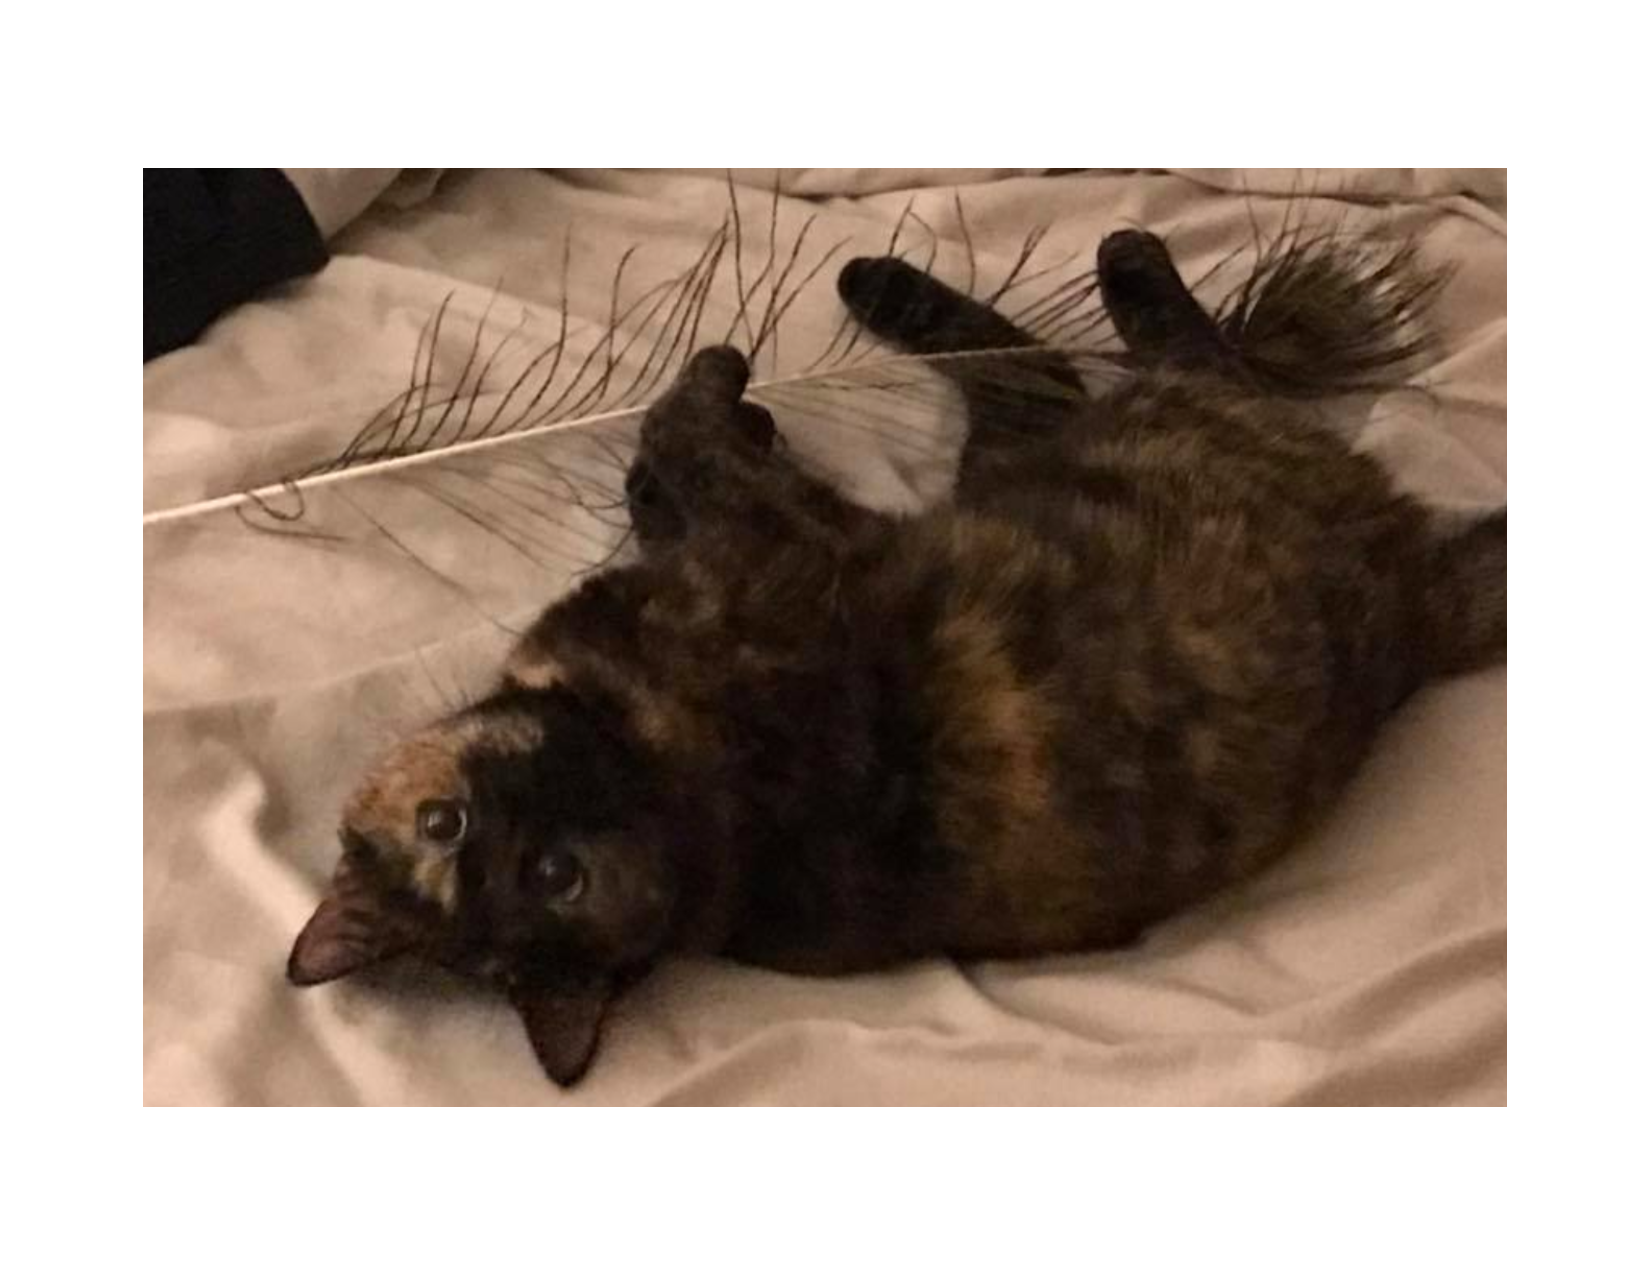
\includegraphics[width=0.6\textwidth,trim=2cm 4cm 2cm 4cm,clip]{fox}
  \caption{Fox Trot}
  \label{fig::fox}
\end{figure}


% *********************** Adding TOC and List of Figures ***********************
\tableofcontents
\listoftables
\listoffigures


%\clearpage
\mainmatter
\renewcommand{\thepage}{\arabic{page}}
% ******************************** Main Matter *********************************
\chapter{Introduction} \label{ch::intro}

More than 100 years ago, Rutherford's famous scattering experiment discovered
the atom was composed of a small but massive nucleus~\cite{Rutherford:1911zz}.
Rutherford scattered relativistic particles off a fixed target and by measuring
the angular products was able to propose the existence of a nucleus.  His
technique provided the blue prints to study the nucleus over the next century
and with higher energies and new probes the nucleus was as well found to have a
substructure.  The nucleus is now known to be composed of protons
and neutrons which are collectively called nucleons.

With still higher energy scattering experiments the nucleons were found to be
composite particles as well.  In 1964 Gell-Mann and Zweig proposed the quark
model to describe the substructure of
nucleons~\cite{GellMann:1964nj,Zweig:1964jf}.  In the quark model the proton is
composed of two u-quarks and a d-quark.  Quarks were defined as elementary
particles with fractional electric charge and a spin of 1/2.  Later Feynman
proposed the parton model to explain the results of deep inelastic scattering
(DIS) experiments~\cite{PhysRevLett.23.1415}.  In the parton model, DIS takes
place between a distribution of partons inside a nucleon.  The parton was
defined as a point like particle which can be either a quark or a gluon.  Later
these two theories were unified by the theory of quantum chromodynamics (QCD)
which describes the nucleon as being held to together by force carrier gluons.
In the QCD model, a nucleon is composed of a distribution of valence quarks
surrounded by sea quarks and gluons.  The valence quarks are responsible for the
charge of the nucleon as the sea quarks occur in quark-antiquark pairs of net
zero electric charge.  QCD is now the accepted theory for describing the
dynamics inside a nucleon.

While there is a theory to describe the quark and gluon interactions, there is
currently no theory to describe the bound dynamics of quarks and gluons inside a
nucleon.  Instead the bound nuclear properties are input as parameters.  High
energy hadron scattering can be factorized as a hard scattering process
multiplied by a soft non-perturbative scattering process.  The hard scattering
can be calculated ab initio using perturbative QCD, while the soft scattering,
on the other hand, is parameterized as the hadron structure or a fragmentation
process.  Both the hadron structure and fragmentation processes are determined
experimentally as either parton distribution functions (PDF) or fragmentation
functions (FF) respectively.  The former describes how quarks and gluons are
bound in a hadron while the latter describes the probability for a quark to
fragment into a detectable hadron.

The quark and gluon parton distribution functions (PDFs) have been determined
with increasing precision from QCD analysis of DIS, Drell-Yan and semi-inclusive
deep inelastic scattering (SIDIS) high energy experiments.  When the scattered
nucleon has large momentum, the PDFs describe the parton distributions in
longitudinal momentum space along the direction of the nucleon's momentum.  The
most recent theories of the nucleon attempt to give a three dimensional
tomographic image of the quark and gluon structure which extend beyond the
longitudinal picture to include transverse effects.  The extended distributions
include either transverse position or transverse momentum to the parton's
longitudinal momentum.  The former are described by generalized parton
distributions (GPD) and the latter are described by transverse momentum
dependent (TMD) PDFs.  This thesis focuses on TMDs.

A unique way to probe TMDs is by studying transverse spin effects.  Polarizing
the nucleon transverse to its momentum gives access to the internal nucleon
structure which cannot be accessed from spin-independent experiments.  As an
example the Sivers TMD PDF is a correlation between transverse spin of the
nucleon and transverse momentum of a constituent parton~\cite{Sivers}.  It
therefore makes sense that the only way to measure the Sivers function is
through transverse spin experiments.

The first TMDs were proposed to explain the results from large single-spin
asymmetries (SSA).  A SSA is defined as a normalized difference between spin
related counts from a given reaction.  One SSA, for example, is the normalized
difference between left and right counts from collisions of a transversely
polarized beam.  This left-right asymmetry was first measured in 1976 and found
to be non-zero in proton-proton collisions~\cite{PhysRevLett.36.929}.  The
Sivers function was proposed to describe large SSAs which lead to a the
theoretical frame work of TMDs and is the subject of this thesis.

This thesis is organized into nine chapters.  Chapter~\ref{ch::theory_exp}
provides the theoretical and experimental background needed to describe the
analysis results in this thesis.  Chapter~\ref{ch::compass} describes the data
taking setup, particularly by describing the experimental apparatus and the
beam.  Chapter~\ref{ch::dc05} gives details on the DC05 large area drift chamber
which was needed for data taking and which the author of this thesis helped
construct and maintain.  Chapter~\ref{ch::alignment} provides details on the
spectrometer alignment which is a crucial preprocessing step for reconstructing
data and which the author of this thesis was responsible for in 2015.
Chapters~\ref{ch::hmanalysis}-~\ref{ch::jpsi} go over the author's analysis
techniques, results and conclusions and chapter~\ref{ch::conclusion} provides a
final summary and conclusion.

\chapter{Theoretical and Experimental Overview} \label{ch::theory_exp}
\ifpdf
\graphicspath{{Chapters/Theory/Figs/}}
\fi

\section{Deep Inelastic Scattering}
To understand the structure of the nucleon it is useful to first introduce the
original process which described the nucleon as having a sub-structure.  This
process is the Deep Inelastic Scattering (DIS) process where a lepton impinges
on a nucleon denoted as

\begin{equation}
l(\ell) + N(P) \rightarrow l(\ell') + X(P_X),
\end{equation}
\noindent
where $l$ denotes a lepton, $N$ denotes a nucleon, $X$ represents all products
not detected and $\ell$, $\ell'$, $P$ and $P_X$ are the four momentum for their
respective lepton or nucleon.  This process is an electromagnetic reaction where
a lepton is scattered via virtual photon exchange with the nucleon.  The
leading order Feynman diagram for this reaction is shown in
Fig.~\ref{fig::DIS_LO}.

\begin{figure}[h!t]
  \centering
  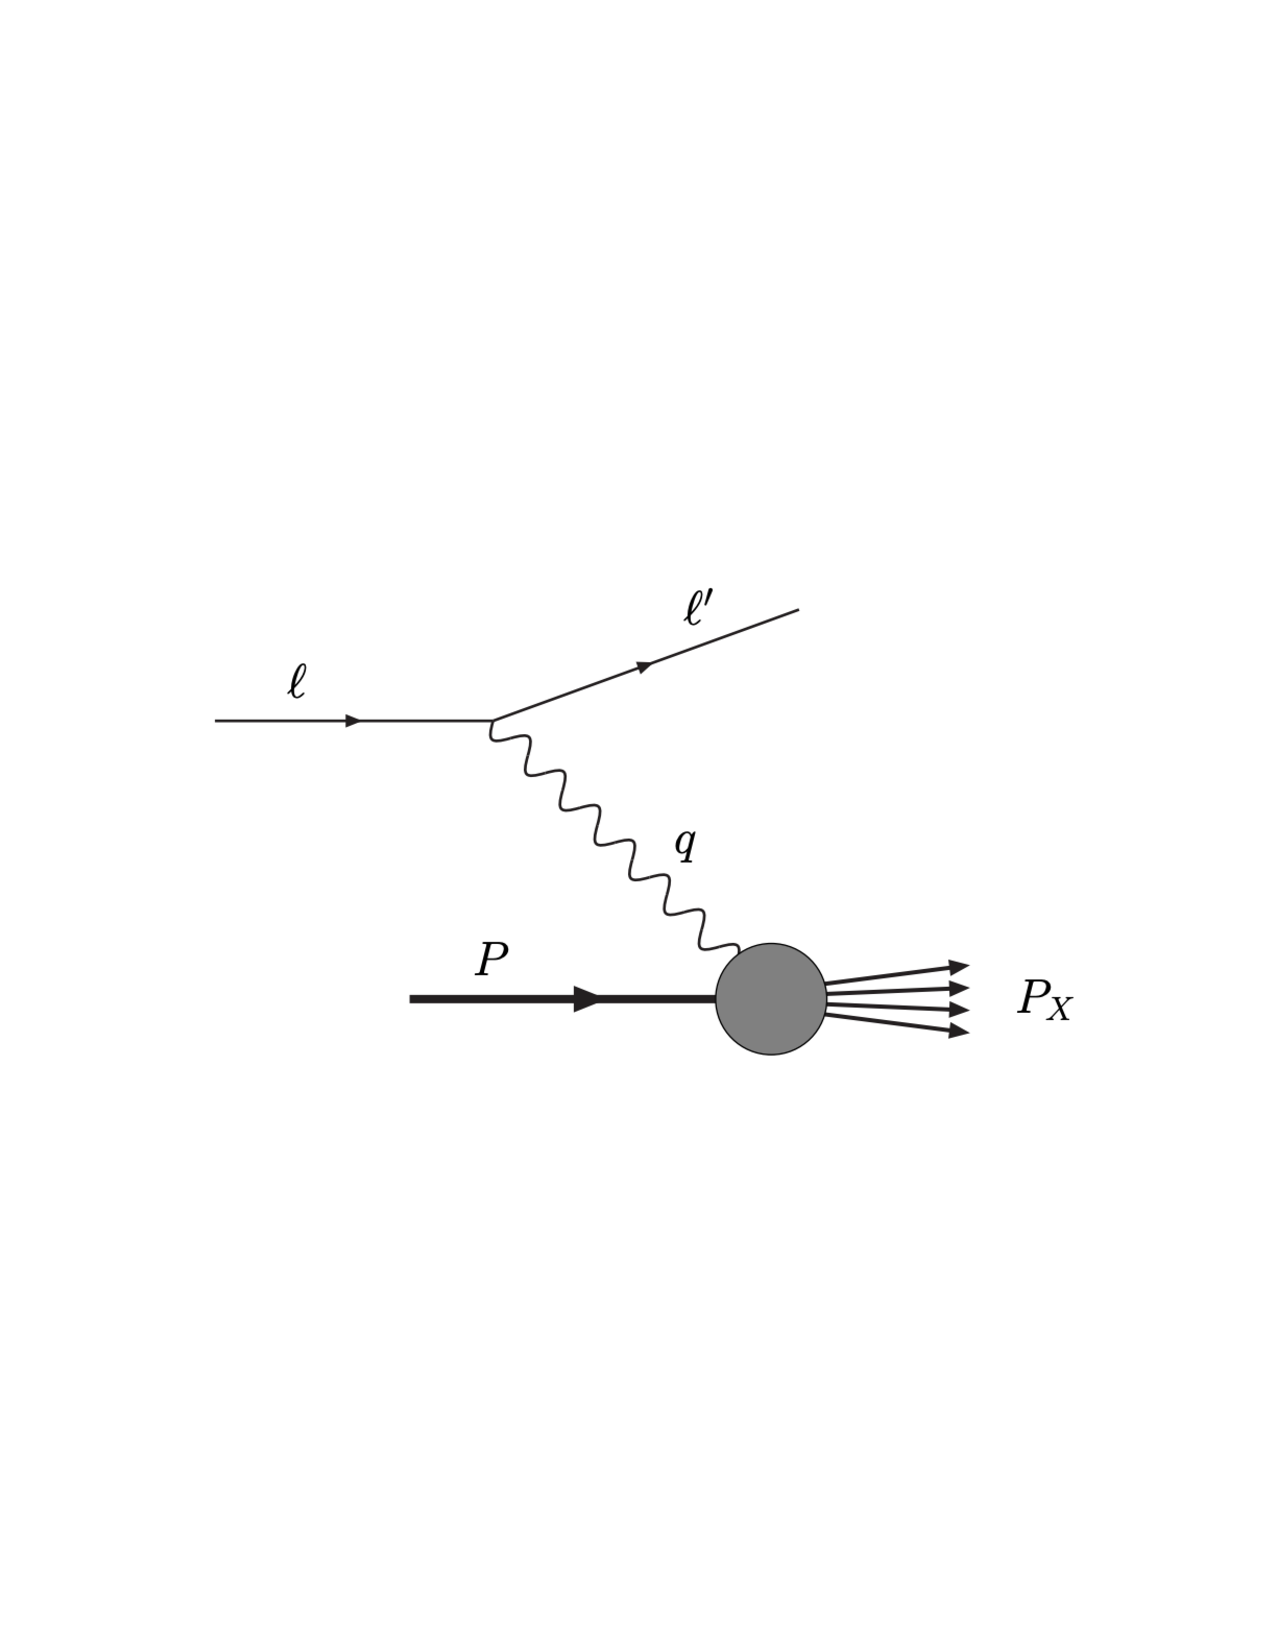
\includegraphics[width=0.5\textwidth, trim=3cm 9cm 3cm 9cm, clip]{DIS_LO}
  \caption{The leading order Feynman diagram for deep inelastic scattering}
  \label{fig::DIS_LO}
\end{figure}

DIS is traditionally studied with a high energy lepton beam and a fixed nuclear
target.  The initial state kinematics are described by

\begin{equation}
  s = (\ell+P)^2 \quad \mathrm{or} \quad E,
\end{equation}
\noindent
where $s$ is the center of mass energy and $E$ is the energy of the lepton beam.
The detected reaction kinematics in the lab frame are described by

\begin{multicols}{2}
  \noindent
  \begin{equation}
    \label{equ::DIS_Q2}
    Q^2 = -q^2 = -(\ell - \ell')^2 \approx EE'(1-\cos\theta )
  \end{equation}
  \begin{equation}
      \label{equ::BjorkenX}
      x = \frac{Q^2}{2P \cdot q} = \frac{Q^2}{2M\nu}
  \end{equation}
\end{multicols}

\begin{multicols}{2}
  \noindent
  \begin{equation}
    \nu = E - E'
  \end{equation} 
  \begin{equation}
    \label{equ::inelasticity}
    y = \frac{P \cdot q}{P \cdot \ell} = \frac{E - E'}{E} = \frac{\nu}{E}
  \end{equation} 
\end{multicols}

\begin{multicols}{2}
  \noindent
  \begin{equation}
    \label{equ::DIS_W}
    W^2 = (P+q)^2
  \end{equation}
\end{multicols}

\noindent
where $q$ is the virtual photon four momentum, $E'$ is the scattered lepton's
energy, $x$ is Bjorken x, $\nu$ is the change in energy of the scattered lepton,
$y$ is the inelasticity and $W^2$ is the invariant mass of the hadron final
state.  In the last relation from Eq.~\ref{equ::DIS_Q2}, $\theta$ is the
scattering angle of the lepton with respect to the beam and the approximation is
only true when the lepton mass is assumed to be zero.  This assumption and the
assumption that a quark's mass is zero will be made throughout this thesis.  In
Eq.~\ref{equ::BjorkenX}, $M$ is the nucleon mass.

In the parton model, section~\ref{sec::parton_model}, $x$ has the interpretation
as being the longitudinal momentum fraction of the struck parton with respect to
its parent hadron and therefore $x$ ranges between 0 and 1.  The inelasticity,
$y$, measures the proportional energy reduction of the lepton and therefore it's
value ranges between 0 and 1.

The process is called deep if $Q^2 >> M^2$ and inelastic if $y < 1$.  For
practical purposes, in experiments, the deep inelastic criteria corresponds to a
$Q^2 > 1~GeV$ and $W^2 > M^2$.  As can be seen in
Eq.~[\ref{equ::DIS_Q2}-\ref{equ::DIS_W}], not all the variables are independent.
DIS is described by two independent variables usually given by ($x$, $Q^2$) or
($x$, $y$).  For reference, in the limit as $y \to \; 1$ the process becomes
elastic scattering and can then be described by only one independent variable.

The differential cross-section for DIS is defined as~\cite{Barone:2001sp}
\begin{equation}
  \label{equ::DIS_xsection}
  \mathrm{d}\sigma =
  \frac{1}{4P\cdot \ell}\frac{e^4}{Q^4} L_{\mu\nu}W^{\mu\nu}
  2\pi\frac{\mathrm{d}^3\ell'}{(2\pi)^32E'}
\end{equation}
\noindent
where $L_{\mu\nu}$ is the leptonic tensor and $W^{\mu\nu}$ is the hadronic
tensor.  The leptonic tensor describes free leptons and can therefore be
calculated in perturbation theory.  It can be decomposed into a systematic
spin-independent tensor and an anti-symmetric spin-dependent tensor.  Summing
over all the possible spins of the lepton beam, the leptonic tensor is

\begin{equation}
  L_{\mu\nu} = 2\Big(\ell_{\mu}\ell'_{\nu} + \ell_{\nu}\ell'_{\mu} -
  g_{\mu\nu}\ell \cdot \ell' \Big) +
  2m\epsilon_{\mu\nu\rho\sigma}s^{\rho}q^{\sigma}
\end{equation}
\noindent
where $m$ is the lepton mass and $s^{\rho}$ is the spin four vector of the
lepton.

Generically the hadronic tensor is defined as
\begin{equation}
  W^{\mu\nu} = \frac{1}{2\pi}
  \int \mathrm{d}^4\xi e^{iq \cdot \xi}
  \langle PS | J^{\mu}(\xi)J^{\nu}(0) | PS \rangle
\end{equation}
\noindent
where $J$ is an electromagnetic current and $|PS \rangle$ represents the nucleon
with momentum $P$ and spin $S$.  The hadronic tensor describes a hadron bound
together by quantum chromo-dynamics (QCD).  As of yet there is no known
technique for calculating the hadronic tensor in a perturbation theory or
otherwise.  Instead the hadronic tensor can be written in the most general
Lorentz invariant form using structure functions to parameterize the
non-perturbative nature of the tensor.  With the use of these structure
functions, the differential DIS cross-section can be written
\begin{equation}
  \label{equ::DIS_diffxsection}
  \frac{\mathrm{d}\sigma}{\mathrm{d}x\mathrm{d}y} =
  \frac{8\pi\alpha^2ME}{Q^4}
  \Big\{
  xy^2F_1(x, Q^2) + \Big(1-y\Big)\frac{F_2(x, Q^2)}{x}
  + c_1(y, \frac{Q^2}{\nu}) g_1(x, Q^2) + c_2(y, \frac{Q^2}{\nu}) g_2(x, Q^2)
  \Big \}
\end{equation}
\noindent
where $\alpha$ is the electromagnetic coupling constant; $F_1$, $F_2$, $g_1$,
$g_2$ are structure functions; and $c_1$ and $c_2$ are functions which depend on
the polarization of the target.  The SLAC collaboration measured the structure
functions, $F_1$ and $F_2$, and found mild variations as a function of
$Q^2$~\cite{Bloom:1969kc,Breidenbach:1969kd}.  This phenomenon now known as
Bjorken scaling lead to the theory of the parton model where the DIS reaction no
longer depends on $Q^2$~\cite{Bjorken:1969ja}.  Fig.~\ref{fig::F2} shows the
$F_2$ structure function which is approximately constant as a function of $Q^2$.

\begin{figure}[h!t]
  \centering
  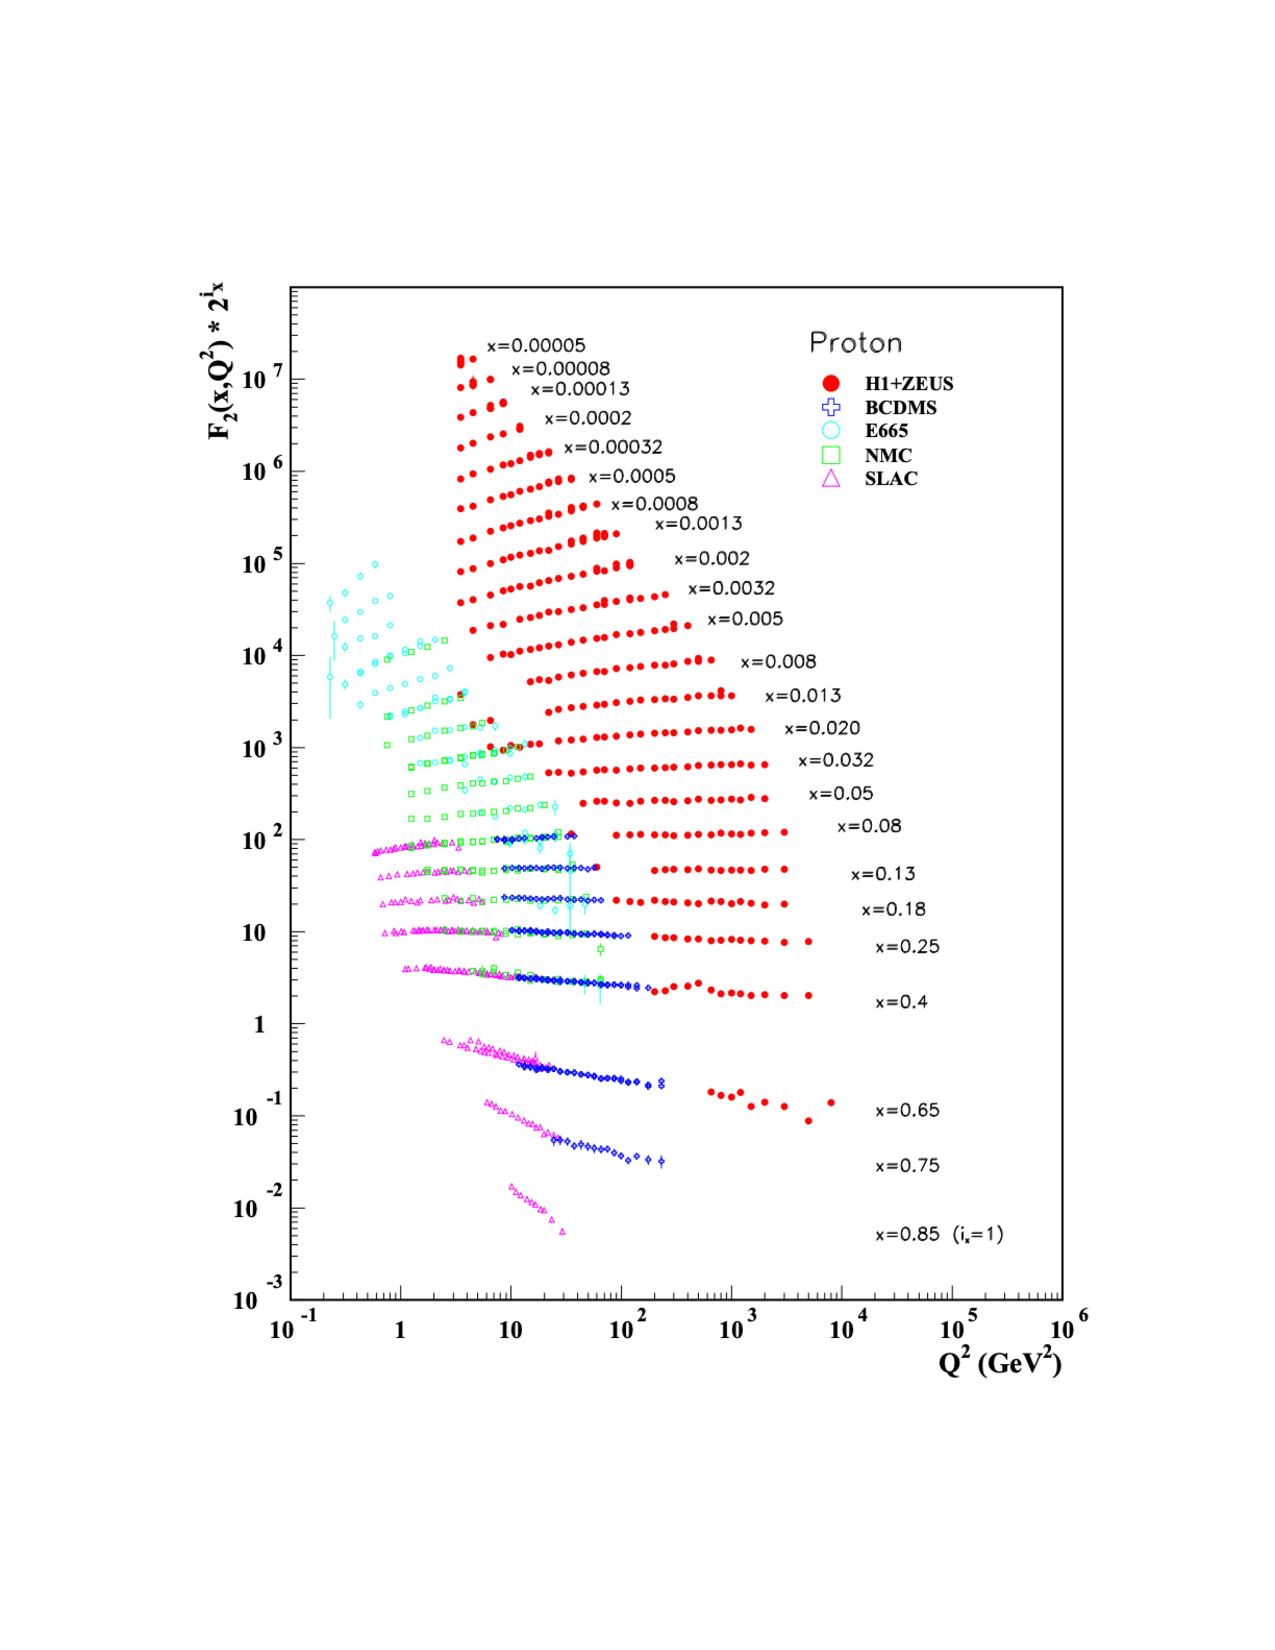
\includegraphics[width=0.5\textwidth, trim=3cm 4cm 3cm 4cm, clip]{F2}
  \caption{The $F_2$ structure function measured by several experiments.  Note
    that the data is shifted up by a factor $2^{i_x}$ to see the $x$ dependence.
    Image taken from~\cite{Tanabashi:2018oca}}
  \label{fig::F2}
\end{figure}


\section{The Parton Model} \label{sec::parton_model}
The parton model is described in an infinite momentum frame which for practical
measurements is defined as the frame where the nucleon is moving with momentum
larger than it's invariant mass.  In the parton model the nucleon, in high
energy scattering processes, is considered to be composed of point like
constituent mass-less particles called partons.  At high energy scattering the
QCD strong force, binding the partons together, becomes asymptotic small and
therefore the partons appear to be free.  The cross-section in DIS can then be
described as a lepton scattering incoherently off a free parton in the nucleon.
In the parton model the hadron tensor for scattering off a quark can be written
as~\cite{Barone:2001sp}

\begin{dmath}
  W^{\mu\nu} = \frac{1}{2\pi} \sum_q e_q^2 \sum_X
  \int \frac{\mathrm{d}^3 P_X}{(2\pi)^32E_X}
  \int \frac{\mathrm{d}^4k}{(2\pi)^4}
  \int \frac{\mathrm{d}^4k'}{(2\pi)^4} \delta(k^{\prime2}) 
       \times [\bar{u}(k')\gamma^{\mu}\langle X | u(k) | PS \rangle] 
       \times [\bar{u}(k')\gamma^{\nu}\langle X | u(k) | PS \rangle]
       \times (2\pi)^4\delta^{(4)}(P-k-P_X)(2\pi)^4\delta^{(4)}(k+q-k'),
\end{dmath}
\noindent
where $e_q$ is the electric charge of quark flavor $q$ and $u(\bar{u})$
is a free Dirac spinor.  This hadronic tensor can be simplified by introducing
the quark-quark correlation matrix as

\begin{equation}
  \Theta_{ij}(k, P, S) =
  \sum_X \int \frac{\mathrm{d}^3 P_X}{(2\pi)^32E_X}(2\pi)^4\delta^{(4)}(P-k-P_X)
  \times \langle PS | \phi_j(0) | X \rangle \langle X | \phi_i(0) | PS \rangle,
\end{equation}
\noindent
where $\phi(\xi) = e^{-ip \cdot \xi}u(p)$ is a quark field.  Using the
quark-quark correlation matrix, the hadronic tensor can be written as

\begin{equation}
  W^{\mu\nu} = \sum_q e_q^2 \int \frac{\mathrm{d}^4k}{(2\pi)^4}
  \int \frac{\mathrm{d}^4k'}{(2\pi)^4} \delta(k^{\prime2})
  (2\pi)^4\delta^{(4)}(k+q-k')\times \mathrm{Tr}
  [ \Theta \gamma^{\mu}\slashed{k'}\gamma^{\nu} ].
\end{equation}
\noindent
In the cases of unpolarized or longitudinally polarized DIS the lead order
contributing terms from the quark-quark correlator
are~\cite{Mulders:1995dh,Boer:1997nt,Bacchetta:2006tn}

\begin{equation}
  \label{equ::simpleQQcorr}
  \Theta = \frac{1}{2}
  \Big(
  f_1(x)\slashed{P} +
  g_{1L}(x)\lambda\gamma_5\slashed{P}
  \Big)
\end{equation}
\noindent
where $\lambda$ is the longitudinal polarization of the hadron.  In this case,
the hadronic tensor simplifies to a symmetric contribution and an anti-symmetric
contribution as~\cite{Barone:2001sp}

\begin{equation}
  \label{equ::simpleHadronTensor}
  W^{\mathrm{symmetric}}_{\mu\nu} = \frac{1}{P\cdot q} \sum_q e_q^2
  \Big( (k_{\mu}+q_{\mu})P_{\nu} + (k_{\nu}+q_{\nu})P_{\mu}-g_{\mu\nu}
  \Big) f_1^q(x),
\end{equation}
\begin{equation}
  W^{\mathrm{anti-symmetric}}_{\mu\nu} =
  \lambda\epsilon_{\mu\nu\rho\sigma}(k_{\nu}+q_{\nu})P^{\rho}\sum_q e^2_q
  g^q_{1L}(x),
  \label{equ::Wantisymmetric}
\end{equation}
\noindent
where in Eq.~\ref{equ::simpleQQcorr}-\ref{equ::Wantisymmetric}, $f_1$ and $g_1$
are parton distribution functions (PDFs).

$f_1$ is interpreted as the quark number density and $g_{1L}$ is interpreted as
the total quark helicity distribution in a hadron.  $f_1$ refers to the density
of unpolarized quarks in a hadron and $g_{1L}$ refers to the net density of
quarks longitudinally polarized in the same longitudinal direction as the
hadron.  To make this explicit, $f_1$ and $g_{1L}$ can be written

\begin{multicols}{2}
  \noindent
  \begin{equation}
    f_1 = f_1^{+} + f_1^{-},
  \end{equation}
  \begin{equation}
    g_{1L} = f_1^{+} - f_1^{-},
  \end{equation}
\end{multicols}
\noindent
where +(-) denotes the helicity.  To be clear while there is a relationship
between the two functions, Eq.~\ref{equ::g1_g1l_relation}, the parton
distribution $g_{1L}$ is not the same as the structure function $g_1$.

The unpolarized quark number density, $f_1$, has been extracted from global
analysis of several experiments~\cite{Rojo_2015}.  Fig.~\ref{fig::NNPDF_10GeV}
shows the current $xf_1$ values and confidence intervals for different quarks
and gluons in the proton.

\begin{figure}[h!t]
  \centering 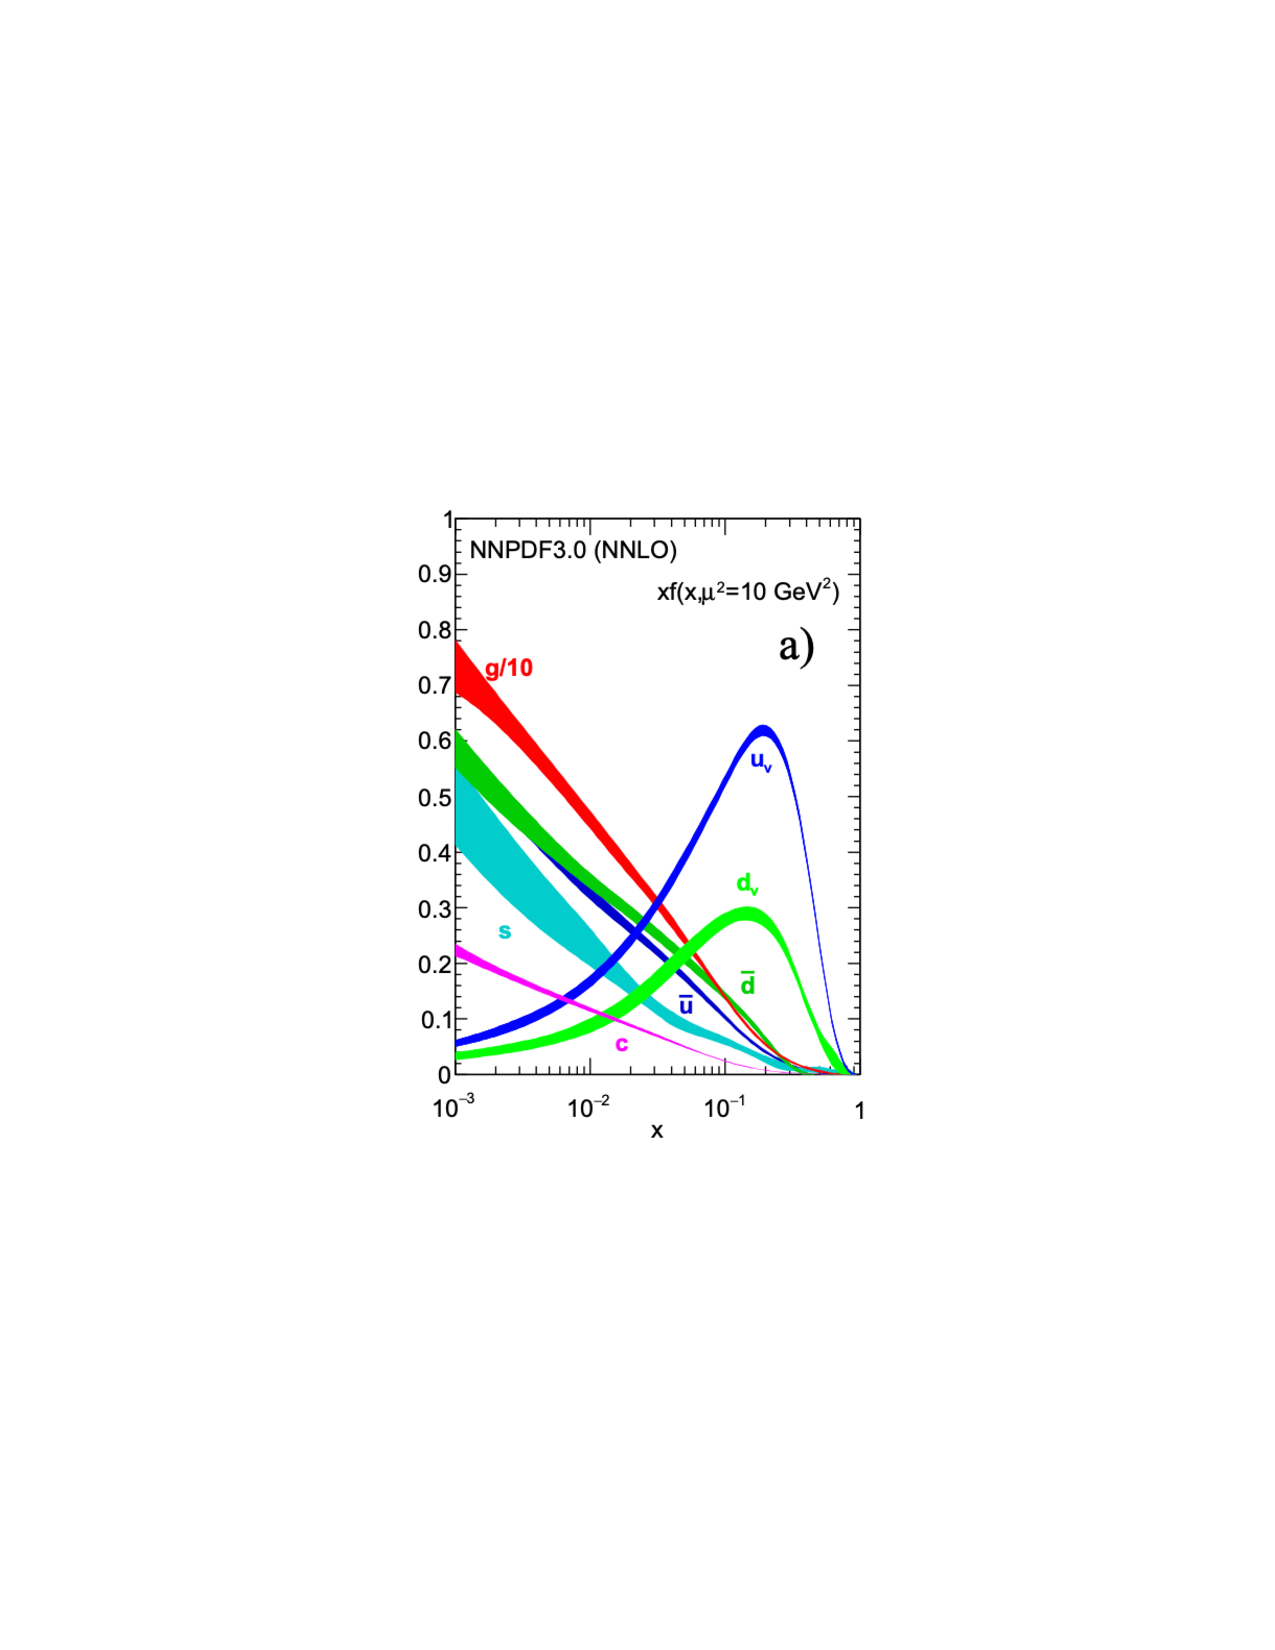
\includegraphics[width=0.5\textwidth,trim=6cm 9cm 6cm 8cm,
    clip]{NNPDF_10GeV}
  \caption{The unpolarized parton distribution functions times the momentum
    fraction.  The different colors correspond to different quarks or gluons.
    Image taken from~\cite{Tanabashi:2018oca}}
  \label{fig::NNPDF_10GeV}
\end{figure}

The longitudinal spin structure, $g_{1L}$, has also been measured at SMC,
HERMES, and COMPASS~\cite{Adeva:1997is,PhysRevLett.92.012005,Savin:2011zz}.  The
global analysis fit is shown in Fig.~\ref{fig::Proton_g1L} using the
parameterizations from NNPDF2014, AAC2008, DSSV2008 and
LSS2010~\cite{Harland-Lang:2016yfn,Abt:2016vjh,Nocera:2014gqa,Hirai:2008aj}.

\begin{figure}[h!t]
  \centering 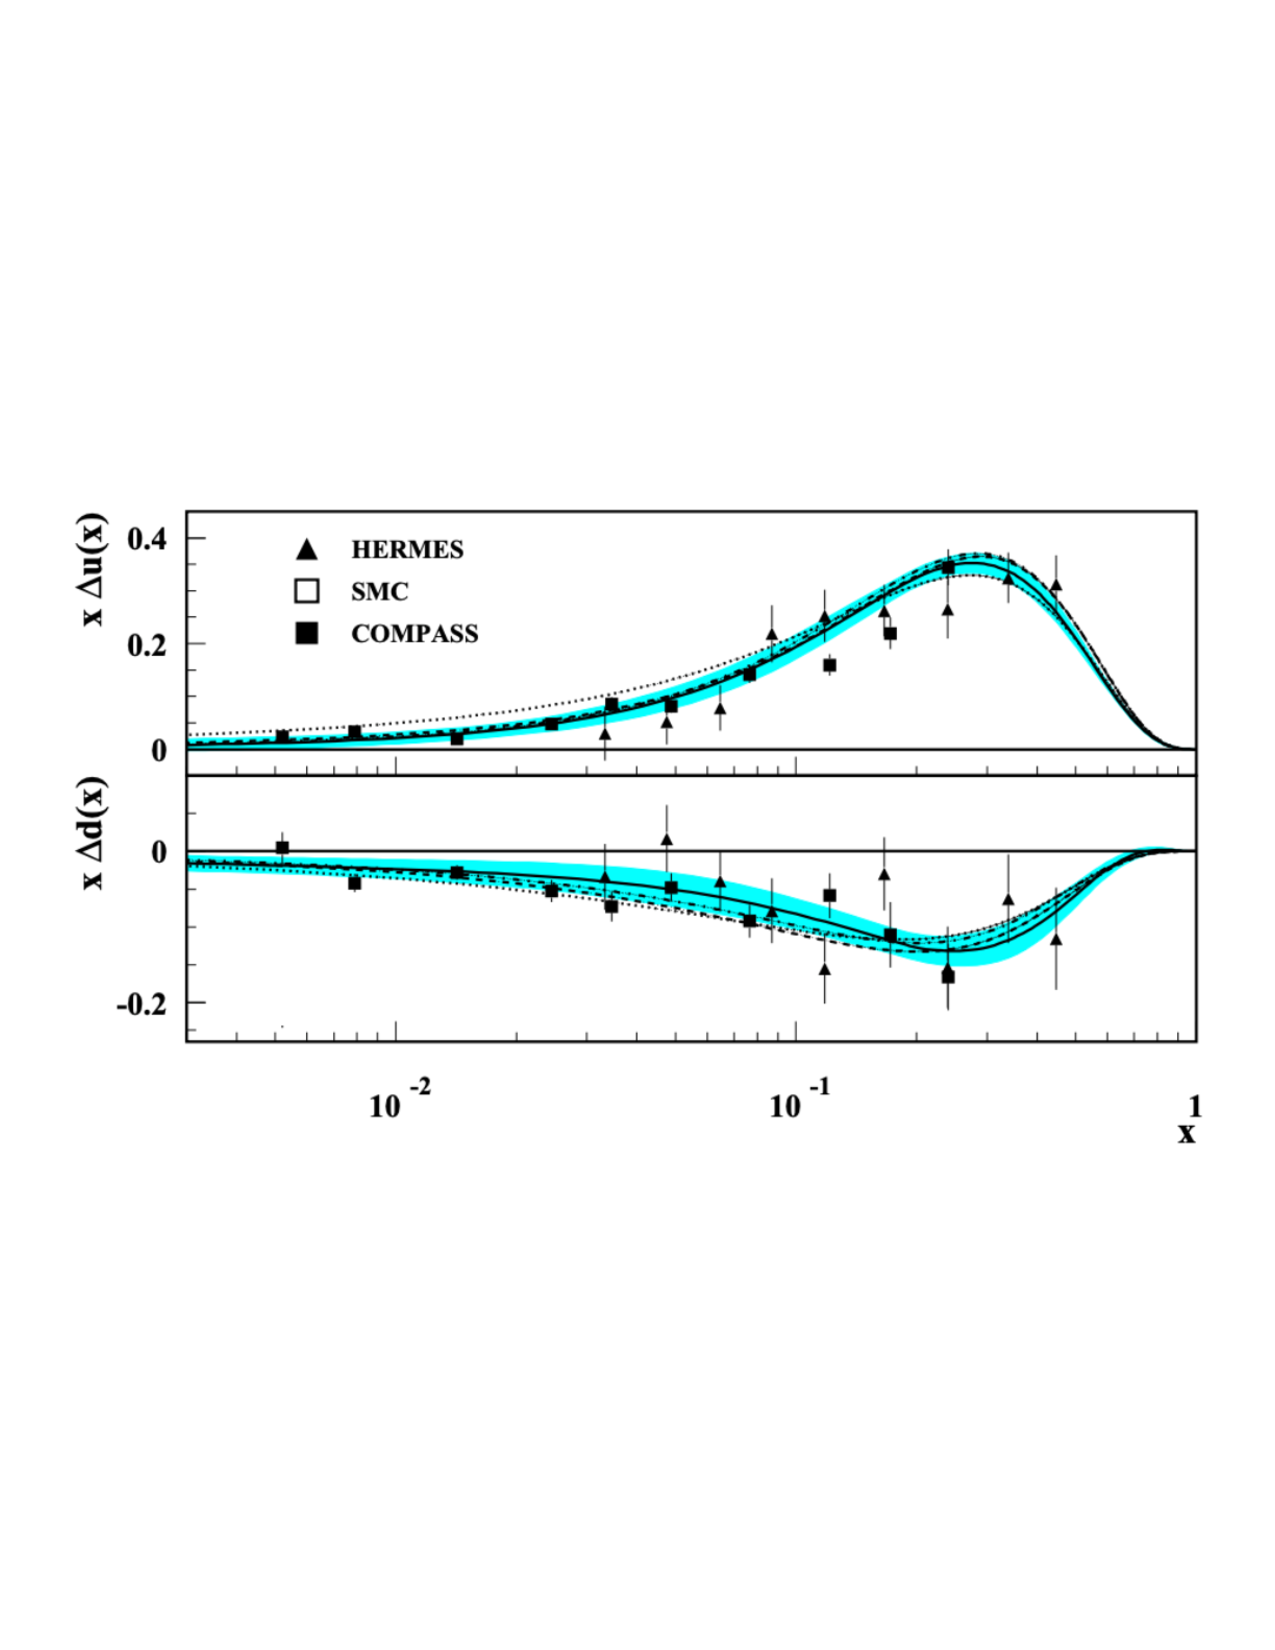
\includegraphics[width=0.5\textwidth,trim=1cm 8cm 1cm 8cm,
    clip]{Proton_g1L}
  \caption{The longitudinally polarized parton distribution functions times the
    momentum fraction for the u-quark (top) and the d-quark (bottom) in a
    proton.  Image taken from~\cite{Tanabashi:2018oca}}
  \label{fig::Proton_g1L}
\end{figure}

In the parton model the structure function $F_1$ and $F_2$ are related to each
other and to the unpolarized quark number as
\begin{equation}
  F_2(x) = 2xF_1(x) = \sum_q e_q^2x\Big(f^q_1 + f^{\bar{q}}_1 \Big)
\end{equation}
which is known as the Callan-Gross relation~\cite{PhysRevLett.22.156}.  As well
the structure function $g_1$ is related to the helicity distribution, $g_{1L}$,
as
\begin{equation}
  g_1(x) = \frac{1}{2} \sum_q e^2_q g_{1L}(x).
  \label{equ::g1_g1l_relation}
\end{equation}


\section{Transverse Momentum Dependence}
In deep inelastic scattering the detected final state lepton is not sensitive to
the parton's transverse momentum.  That is when measuring the DIS
cross-section, all transverse parton momentums are possible which therefore
means the scattered parton's transverse momentum is integrated over.  As a
result, DIS cannot be used to study parton's transverse momentum dependence.
The Drell-Yan process~\ref{sec::DY} and the SIDIS process~\ref{sec::SIDIS}
however are sensitive to the internal transverse momentum of the partons.  In
the limit of small transverse momentum compared to the virtual photon momentum,
the most generic leading order quark-quark correlator including the transverse
parton momentum can be
written~\cite{Mulders:1995dh,Boer:1997nt,Bacchetta:2006tn}

\begin{dmath}
  \label{equ::GeneralQQcorrelator}
  \Theta = \frac{1}{2}\Big[ f_1(x,k_{\bot})\slashed{P} +
    \frac{1}{M}h_1^{\bot}(x,k_{\bot})\sigma^{\mu\nu}k_{\mu}P_{\nu} +
    g_{1L}(x,k_{\bot})\lambda\gamma_5\slashed{P} +
    \frac{1}{M}g_{1T}(x,k_{\bot})\gamma_5\slashed{P}(k_{\bot} \cdot S_{\bot}) +
    \frac{1}{M}h_{1L}(x,k_{\bot})\lambda
    i\sigma_{\mu\nu}\gamma_5P^{\mu}k_{\bot}^{\nu} +
    h_1(x,k_{\bot})i\sigma_{\mu\nu}\gamma_5P^{\mu}S_{\bot}^{\nu} +
    \frac{1}{M^2}h_{1T}^{\bot}(x,k_{\bot})i\sigma_{\mu\nu}\gamma_5P^{\mu} \Big(
    k_{\bot} \cdot S_{\bot}k_{\bot}^{\nu} - \frac{1}{2}k_{\bot}^2S_{\bot}^{\nu}
    \Big ) +
    \frac{1}{M}f_{1T}^{\bot}(x,k_{\bot})\epsilon^{\mu\nu\rho\sigma}\gamma_{\mu}P_{\nu}k_{\rho}S_{\sigma}
    \Big],
\end{dmath}
\noindent
where $k_{\bot}$ denotes the transverse parton momentum and $S_{\bot}$ denotes
the transverse hadron spin.  Eq.~\ref{equ::GeneralQQcorrelator} includes eight
transverse momentum dependent (TMD) PDFs which are functions of $x$ and
$k_{\bot}$.

The notation used to depict the TMD functions is the so-called Amsterdam
notation.  The letters represent the different quark polarizations where
$f,\;g,\;h$ stand for unpolarized, longitudinally polarized and transversely
polarized respectively.  The subscript 1 denotes leading order and the
subscripts $T$ and $L$ denote a transversely polarized hadron and a
longitudinally polarized hadron respectively.  Finally the superscript $\bot$
denotes that the distribution is the coefficient of a term where the in which
the parton's transverse momentum Lorentz indices are not contracted.
Fig.~\ref{fig::TMDs} organizes the TMDs by nucleon and quark polarizations and
gives a visual of each TMD's interpretation.

\begin{figure}[h!t]
  \centering
  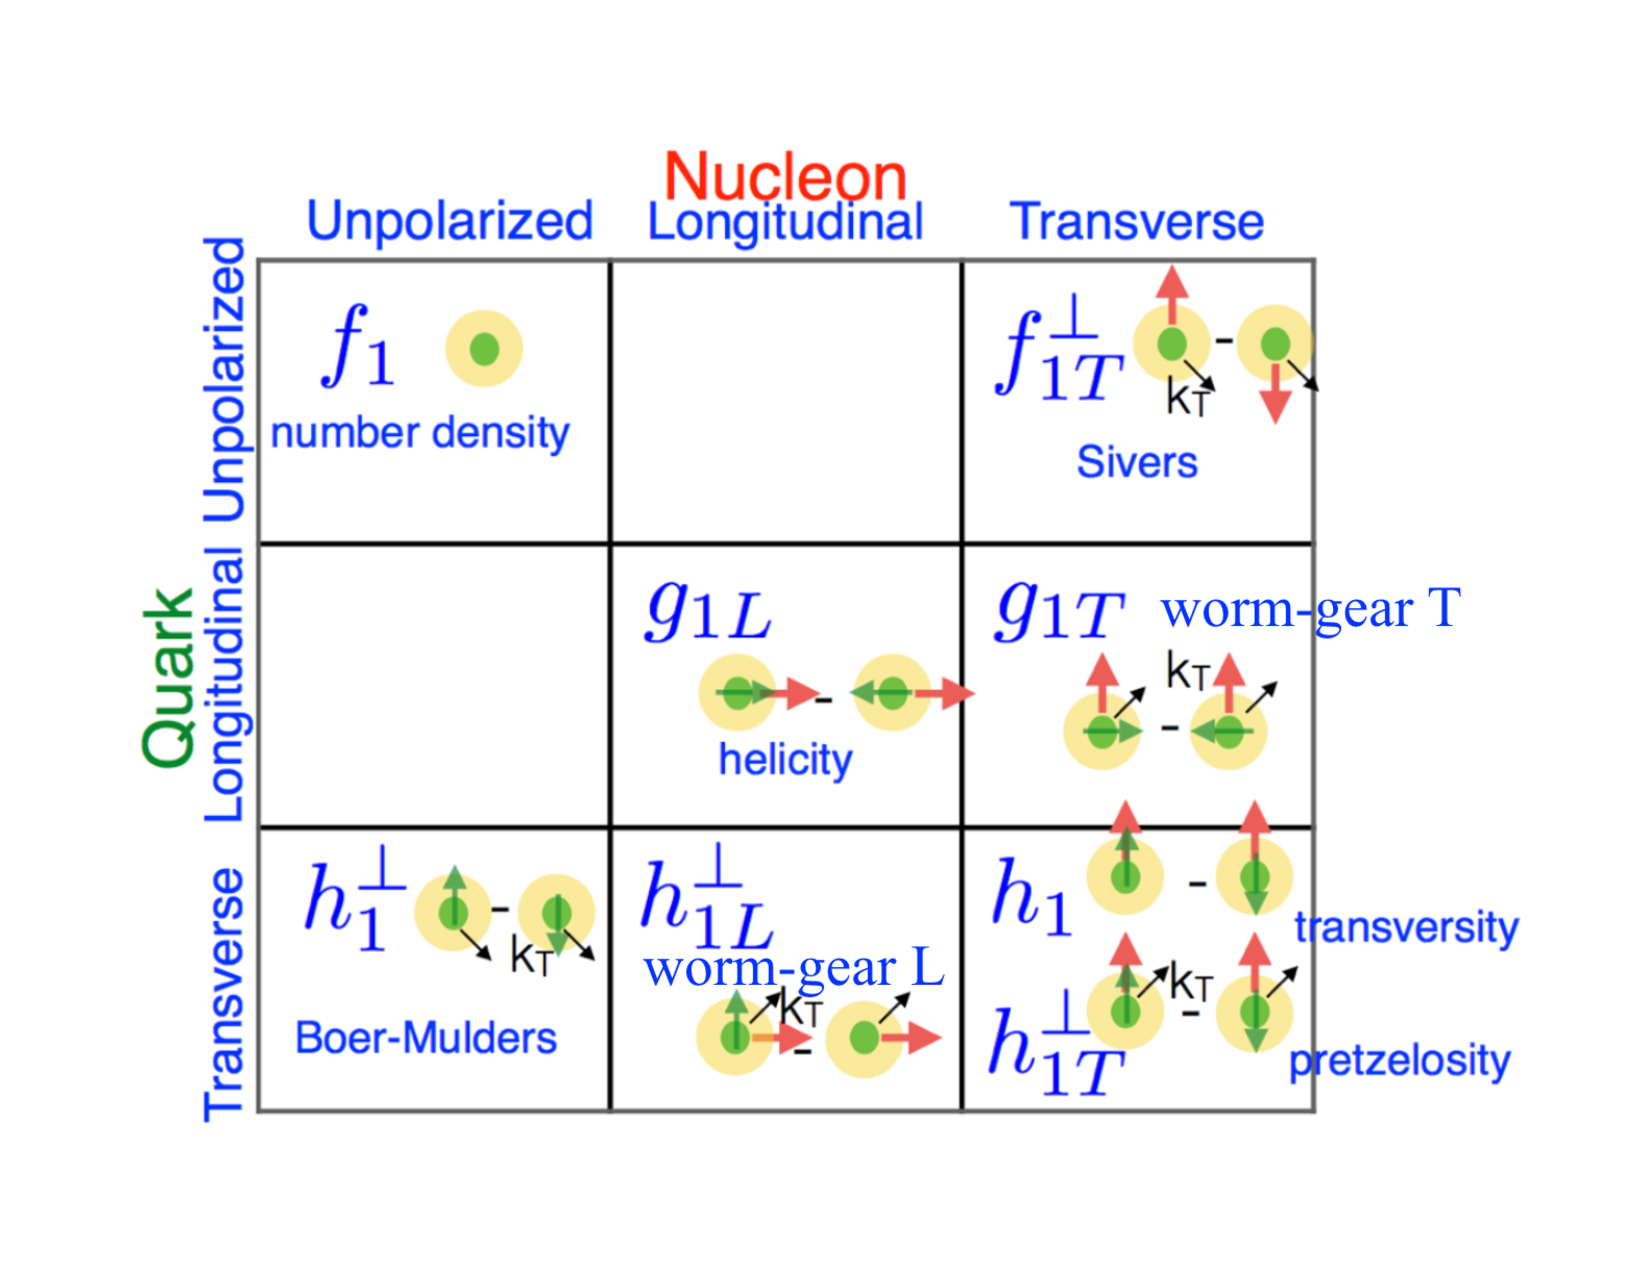
\includegraphics[width=0.6\textwidth, trim=2cm 2cm 2cm 2cm,clip]{TMDs}
  \caption{The eight TMDs needed to describe a spin 1/2 nucleon at leading
    order.  The columns represent the different nucleon polarizations and the
    rows represent the different quark polarizations.  The individual figures
    give a visual representation of the TMD's interpretation.}
  \label{fig::TMDs}
\end{figure}

The TMD functions needed to describe Drell-Yan scattering from a transversely
polarized target, as in the data taking conditions in this thesis are: the
Sivers function, the Boer-Mulders function, the transversity function and the
pretzelosity function.

\subsection{Sivers and Boer-Mulders Distributions}
The Sivers TMD, {\siv}, was first purposed to explain large nucleon
spin-dependent asymmetries~\cite{Sivers}.  The interpretation of the Sivers,
{\siv}, TMD is that it gives a correlation between transverse spin of the parent
hadron and transverse momentum of the scattered parton.  When viewing the hadron
in the direction opposite to it's momentum and using the sign conventions in
this thesis, if {\siv} is positive then it is expected that there are more
partons with momentum pointing left than pointing to the right.  A non-zero
{\siv} then implies that the bound partons in a transversely polarized hadron
are traveling transverse to the hadron's momentum which can intuitively make
senses if the partons have orbital angular momentum.  As of yet however, there
is no theoretical link between orbital angular momentum and the Sivers function.

The Boer-Mulders TMD PDF, $h_1^{\perp}$, was proposed in 1998 as a correlation
between the transverse momentum and the transverse spin of a parton inside an
unpolarized hadron~\cite{Boer:1997nt}.  The Boer-Mulders function is interpreted
as a difference between quarks with transverse momentum and transverse spin up
and quarks with transverse momentum and transverse spin down in an unpolarized
hadron.  It is not hard to realized that changing the chirality of transversely
polarized quarks in an unpolarized hadron would flip the sign of the
Boer-Mulders function which therefore means the Boer-Mulders function is chiral
odd.  Chiral odd functions can only be non-zero when convoluted with another
chiral odd function as is the case when the Boer-Mulders function appears in
either the SIDIS or Drell-Yan cross-section.

The most surprising fact about the Sivers and Boer-Mulders functions is that
they both changes sign under naive time reversal.  Naive time reversal is
defined as reversing time but not swapping initial and final
states~\cite{Bacchetta:2006tn}.  The Sivers and Boer-Mulders functions are
therefore said to be T-odd functions, and as a result, were originally believe
to be forbidden correlations.  However it was shown that the Sivers function
could be non-zero from gluon exchange during the initial state in the Drell-Yan
process and gluon exchange during the final state in the SIDIS
process~\cite{Brodsky:2002cx,Brodsky:2002rv}.  Most surprisingly, it was shown
that a non-zero Sivers function and a non-zero Boer-Mulders function are
expected to have opposite sign in SIDIS and Drell-Yan~\cite{collins_2002}.  That
is

\begin{align}
  f_{1T}^{\bot} |_{Drell-Yan} &= - f_{1T}^{\bot} |_{SIDIS}, \\
  h_{1}^{\bot} |_{Drell-Yan} &= - h_{1}^{\bot} |_{SIDIS}.
\end{align}

\subsection{Transversity and Pretzelosity}
Unlike the Sivers and Boer-Mulders TMDs, the transversity, $h_1(x, k_T)$, and
pretzelosity, $h_{1T}^{\bot}$, TMDs are predicted to be universal functions of a
spin 1/2 hadron.  The transversity is defined for transversely polarized hadrons
as the difference between quarks polarized in the same direction as their parent
hadron and quarks polarized in the opposite direction to their parent hadron.
The transversity distribution is then similar to the helicity distribution,
$g_{1L}$, but for transverse polarizations.  The pretzelosity function is a
correlation between transversely polarized partons and their transverse momentum
in a transversely polarized hadron.  As with the Boer-Mulders TMD, both the
transversity and the pretzelosity TMDs are chiral odd and are therefore
convoluted with another chiral odd function.


\section{Semi-Inclusive Deep Inelastic Scattering} \label{sec::SIDIS}
Semi-Inclusive Deep Inelastic Scattering (SIDIS) is the process where a lepton
scatters electromagnetically off a nucleon and subsequently the scattered lepton
and at least one scattered hadron are detected.  As the name implies, SIDIS is
related to the DIS reaction only SIDIS includes the addition of a detected
hadron.  SIDIS is denoted as

\begin{equation}
  l(\ell, \lambda_l) + N(P, S) \rightarrow l(\ell') + h(P_h) + X(P_X),
\end{equation}
\noindent
where $\lambda_l$ is the helicity of the incoming lepton, $S$ is the spin of the
nucleon, $h$ is the detected hadron and $P_h$ is the detected hadron's four
momentum.  The leading order one photon exchange Feynman diagram for the SIDIS
process is shown in Fig.~\ref{fig::SIDIS_LO}.

\begin{figure}[h!t]
  \centering
  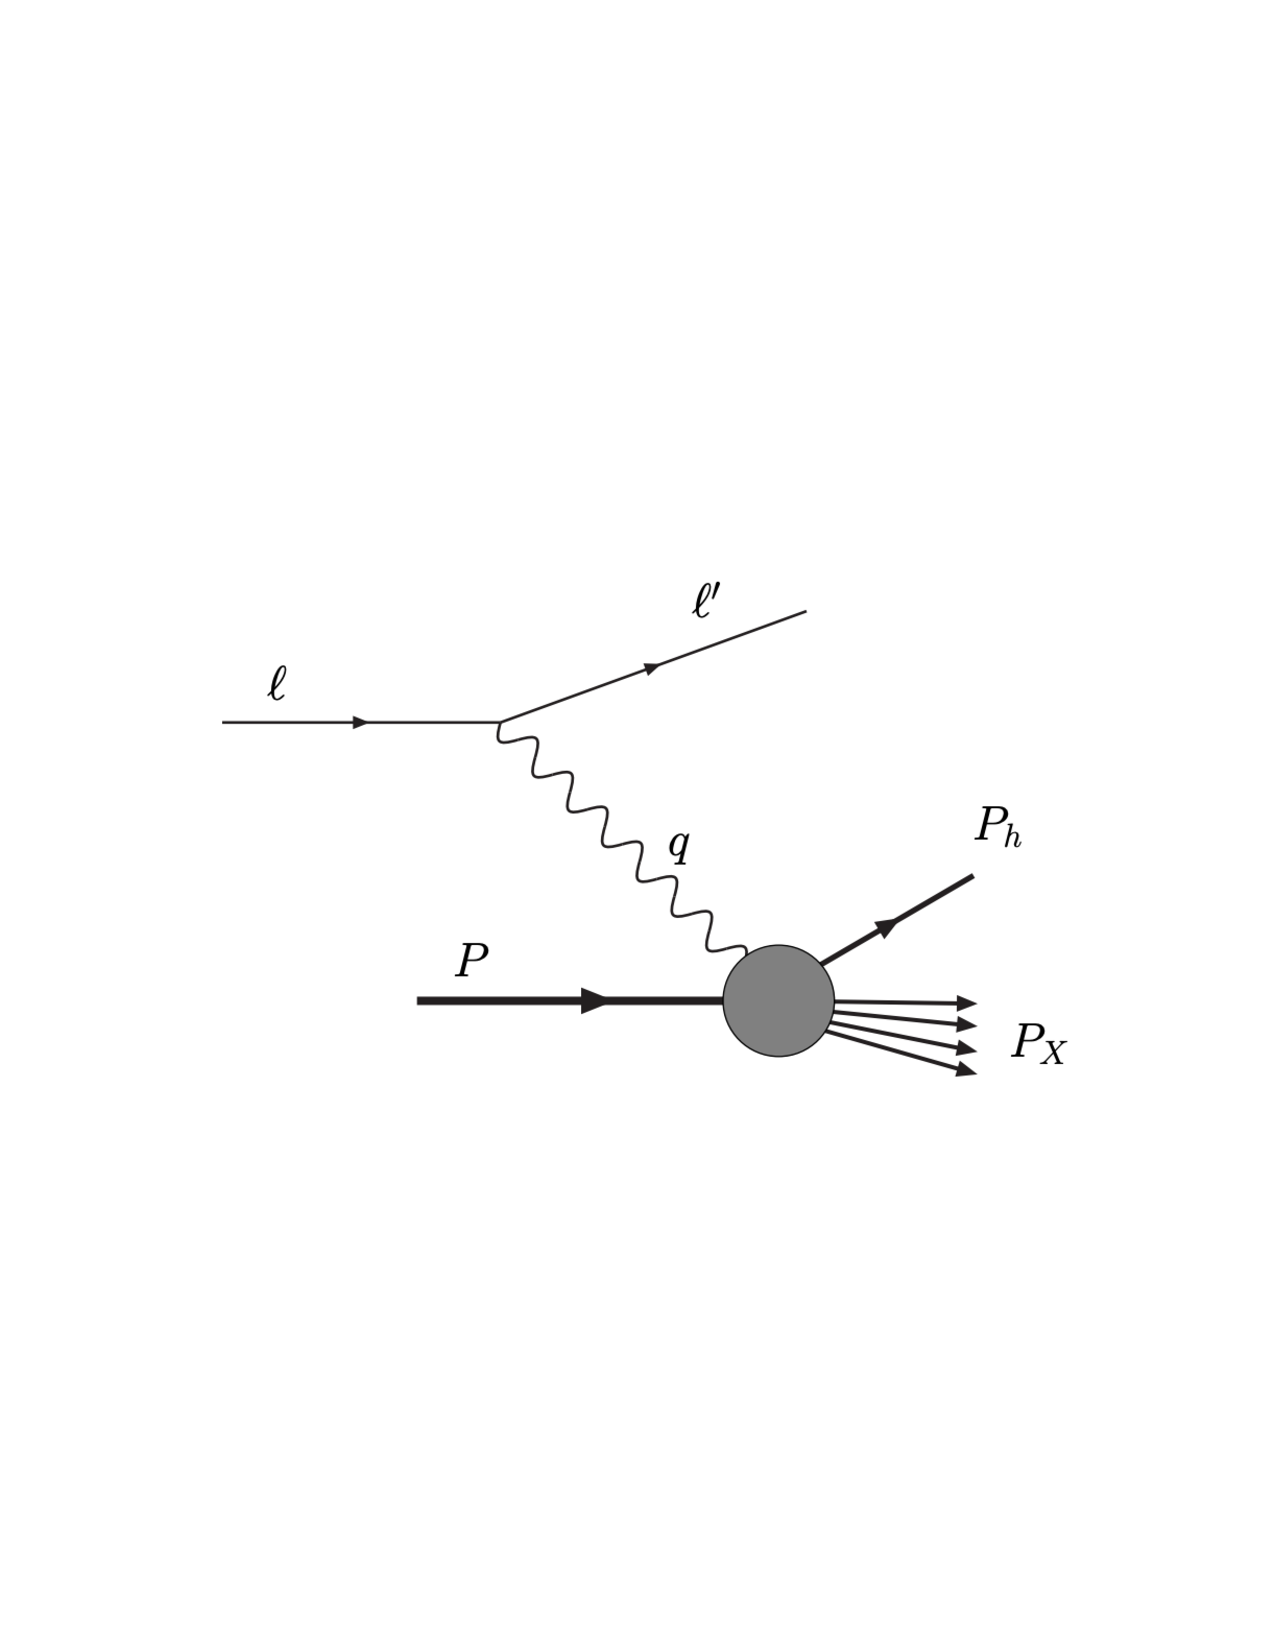
\includegraphics[width=0.5\textwidth, trim=3cm 9cm 3cm 9cm, clip]{SIDIS_LO}
  \caption{The semi-inclusive deep inelastic scattering leading order Feynman
    diagram}
  \label{fig::SIDIS_LO}
\end{figure}

In addition to the kinematic variables used to describe DIS,
Eq.~[\ref{equ::DIS_Q2}-\ref{equ::DIS_W}], one more variable is needed to
describe the SIDIS process,
\begin{equation}
  z = \frac{P \cdot P_h}{P \cdot q} \quad \substack{lab \\frame\\ =} \quad
  \frac{E_h}{E-E'},
\end{equation}
\noindent
which is interpreted as the fraction of possible energy the detected hadron
can obtain.  The transverse spin-dependent SIDIS cross-section can be described
in a model independent way using structure functions as~\cite{Bacchetta:2006tn}

\begin{align}
  \frac{d\sigma}{dx \, dy\, d\psi \,dz\, d\phi_h\, d P_{h\perp}^2} &=
  \frac{\alpha^2}{x y Q^2}\,
  \frac{y^2}{2\,(1-\varepsilon)}\,  \biggl( 1+\frac{\gamma^2}{2x} \biggr)\,
  \Biggl\{
  F_{UU ,T}
  + 
  \varepsilon
  F_{UU ,L}
  + \sqrt{2\,\varepsilon (1+\varepsilon)}\,\cos\phi_h\,
  F_{UU}^{\cos\phi_h}
  \nonumber \\  & 
  + \varepsilon \cos(2\phi_h)\, 
  F_{UU}^{\cos 2\phi_h}
  + \lambda_l\, \sqrt{2\,\varepsilon (1-\varepsilon)}\, 
  \sin\phi_h\, 
  F_{LU}^{\sin\phi_h}
  \phantom{\Bigg[ \Bigg] }
  \nonumber \\  & 
  + |S_\perp|\, \Bigg[
    \sin(\phi_h-\phi_S)\,
    \Bigl(F_{UT ,T}^{\sin\left(\phi_h -\phi_S\right)}
    + \varepsilon\, F_{UT ,L}^{\sin\left(\phi_h -\phi_S\right)}\Bigr)
    \nonumber \\  & \quad  \qquad \qquad
    + \varepsilon\, \sin(\phi_h+\phi_S)\, 
    F_{UT}^{\sin\left(\phi_h +\phi_S\right)}
    + \varepsilon\, \sin(3\phi_h-\phi_S)\,
    F_{UT}^{\sin\left(3\phi_h -\phi_S\right)}
    \phantom{\Bigg[ \Bigg] }
    \nonumber \\  & \quad \qquad \qquad
    + \sqrt{2\,\varepsilon (1+\varepsilon)}\, 
    \sin\phi_S\, 
    F_{UT}^{\sin \phi_S }
    + \sqrt{2\,\varepsilon (1+\varepsilon)}\, 
    \sin(2\phi_h-\phi_S)\,  
    F_{UT}^{\sin\left(2\phi_h -\phi_S\right)}
    \Bigg]
  \nonumber \\  &
  + |S_\perp| \lambda_l\, \Bigg[
    \sqrt{1-\varepsilon^2}\, \cos(\phi_h-\phi_S)\, 
    F_{LT}^{\cos(\phi_h -\phi_S)}
    +\sqrt{2\,\varepsilon (1-\varepsilon)}\, 
    \cos\phi_S\, 
    F_{LT}^{\cos \phi_S}
    \nonumber \\  & \quad \qquad \qquad
    +\sqrt{2\,\varepsilon (1-\varepsilon)}\, 
    \cos(2\phi_h-\phi_S)\,  
    F_{LT}^{\cos(2\phi_h - \phi_S)}
    \Bigg] \Biggr\},
  \label{equ::SIDISxsect}
\end{align}
\noindent
where
\begin{equation}
  \varepsilon =
  \frac{1-y-\frac{1}{4}\gamma^2y^2}{1-y+\frac{1}{2}y^2+\frac{1}{4}\gamma^2y^2},
\end{equation}
\noindent
and $\gamma = \frac{2Mx}{Q}$, $\psi$ is the azimuthal scattering angle of the
lepton around the lepton beam with respect to the transverse spin direction of
the target and where this cross-section is defined in the $\gamma$-nucleon
reference frame.  The $\gamma$-nucleon reference system is a lab frame where
the virtual photon is along the z-axis and the xz-plane is determined by the
lepton plane.  Fig.~\ref{fig::gammaNucleonFrame} shows the $\gamma$-nucleon lab
frame and the relevant azimuthal angles.

\begin{figure}[h!t]
  \centering 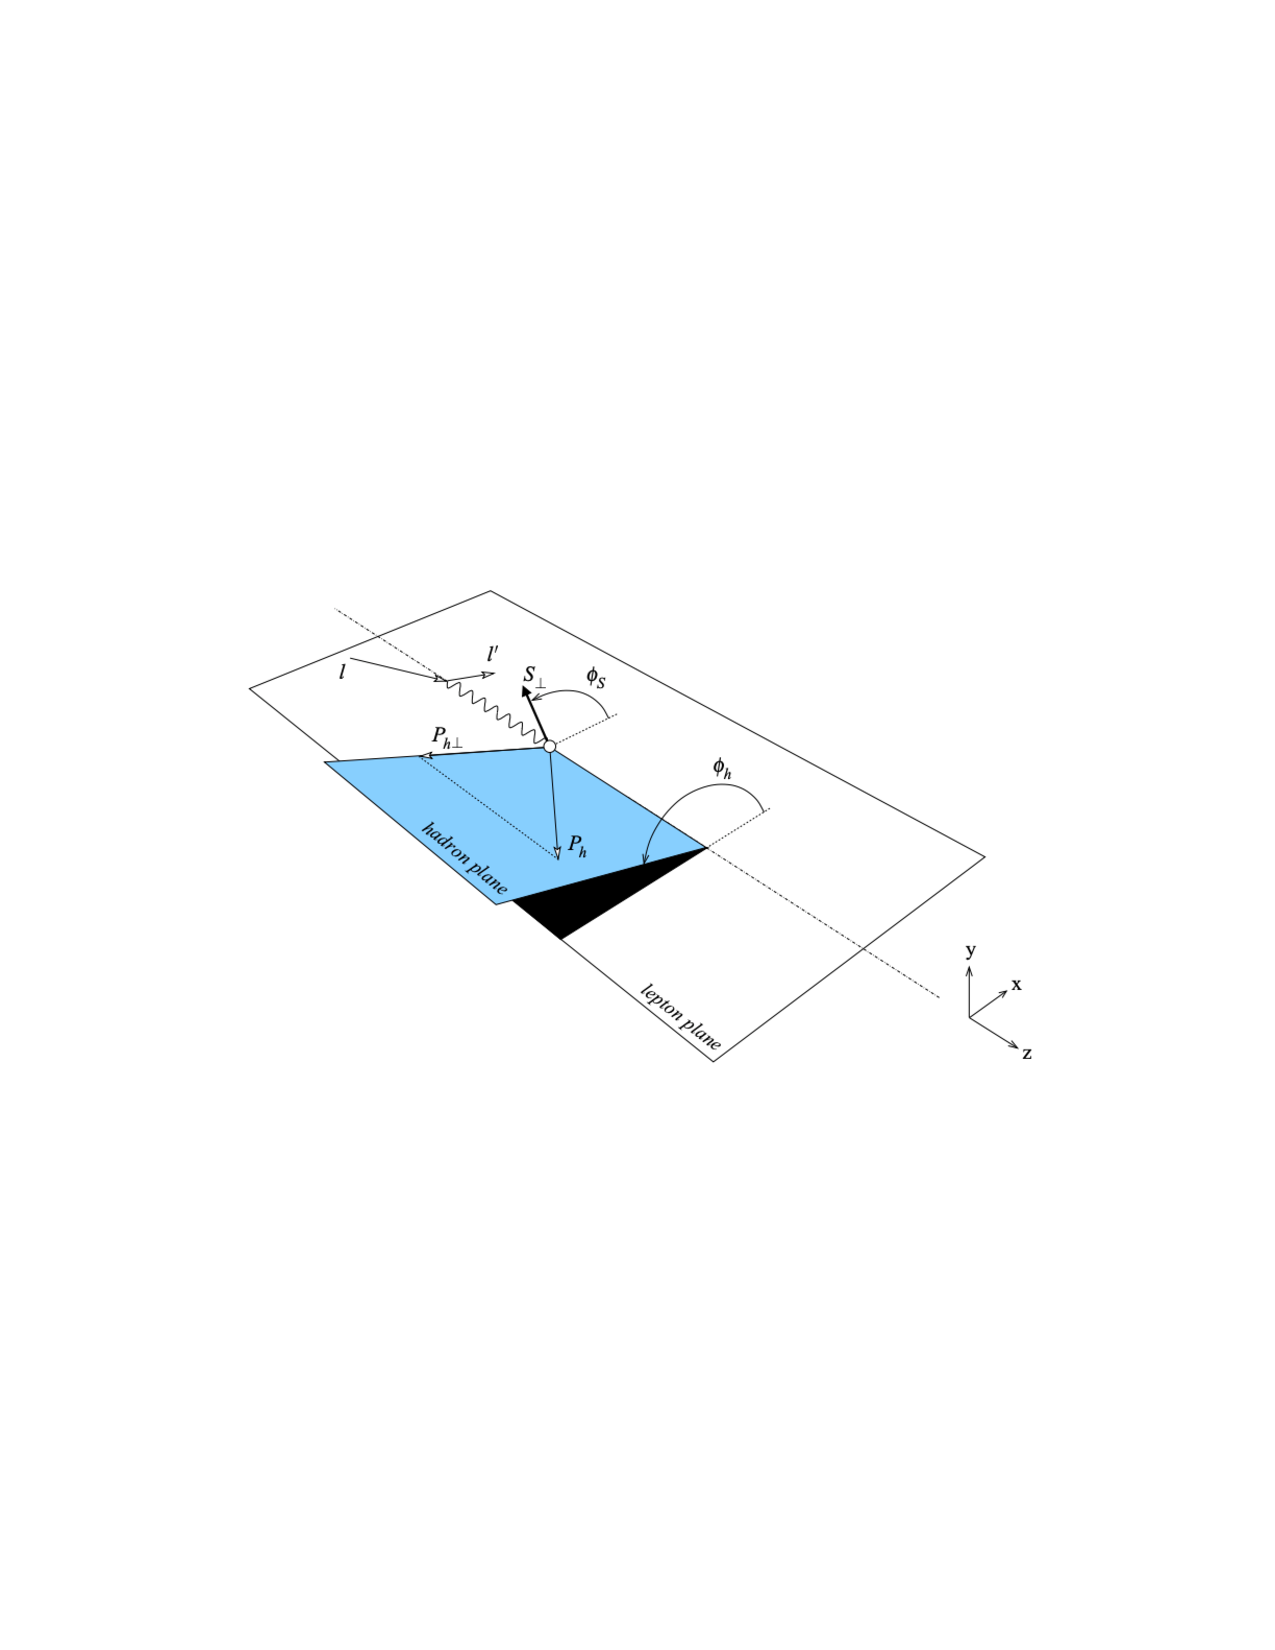
\includegraphics[width=0.6\textwidth,trim=3cm 9cm 3cm 8cm,
    clip]{gammaNucleonFrame}
  \caption{The $\gamma$-nucleon lab frame where the target nucleon is at rest
    and the virtual photon is along the z-axis.  The lepton scattering plane
    defines the xz-plane where the outgoing lepton defines the positive
    x-direction.  This image was taken from~\cite{Bacchetta:2006tn}.}
  \label{fig::gammaNucleonFrame}
\end{figure}

The 14 structure functions in Eq.~\ref{equ::SIDISxsect} are coefficients to the
azimuthal angles from the $\gamma$-nucleon reference frame.  The structure
functions are label as $F$ where the superscript denotes which azimuthal angle
coefficient they correspond to and the three subscripts represent the beam,
target and virtual photon polarization from left to right respectively.  The
subscript polarizations are $U$ for unpolarized, $L$ for longitudinally
polarized and $T$ for transversely polarized.  The cross-section,
Eq.~\ref{equ::SIDISxsect}, is determined similarly to the DIS
cross-section, Eq.~\ref{equ::DIS_diffxsection}, in that structure functions are
used to generically parameterize the hadronic tensor.

In the TMD regime the structure functions are related to TMD functions and
fragmentation functions (FF).  For SIDIS, the TMD regime is defined as the
detected hadron's transverse momentum being small compared to the virtual photon
momentum, $P_{hT} << Q$.  Then in this regime the model independent structure
functions are equal to a convolution of a TMD and a FF where the
convolution is defined as

\begin{equation}
  \label{equ::SIDIS_conv}
{\cal C}\bigl[ w(p_T,k_T) f D \bigr] = x \sum_q e_q^2 \int d^2 p_T d^2 k_T
\delta^{(2)}\bigl(p_T - k_T - P_{h \perp}/z \bigr) w(p_T,k_T)
f^q(x,p_T^2)D^q(z,k_T^2),
\end{equation}
\noindent
where $w$ is a weight $f$ is a TMD function and $D$ is a FF.  For the structure
functions related to transverse target polarization, the relations between
structure functions and TMDs at leading order are~\cite{Bacchetta:2006tn}

\begin{align}
  \label{equ::F_UUTsinphihphis}
  F_{UT ,T}^{\sin\left(\phi_h -\phi_S\right)} &=
  {\cal C}\biggl[-\frac{\hat{h} \cdot p_T}{M} f_{1T}^{\perp } D_1\biggr]
  &\propto f_{1T}^{\perp } \otimes D_1, \\
  F_{UT ,L}^{\sin\left(\phi_h -\phi_S\right)} &= 0,\\
  F_{UT}^{\sin(\phi_h +\phi_S)} &=
  {\cal C}\biggl[-\frac{\hat{h}\cdot k_T^{}}{M_h} h_{1} H_1^{\perp }\biggr]
  &\propto h_{1} \otimes H_1^{\perp },\\
  F_{UT}^{\sin(3\phi_h -\phi_S)} &=
  {\cal C}\biggl[ \frac{2 \bigl(\hat{h}\cdot
      p_T \bigr) \bigl( \bm{p}_T\cdot k_T^{} \bigr) +\bm{p}_T^2
      \bigl(\hat{h}\cdot k_T^{} \bigr) -4 (\hat{h}\cdot p_T)^2 (\hat{h}\cdot
      k_T^{})}{2 M^2 M_h} h_{1T}^{\perp } H_1^{\perp }\biggr]
  &\propto h_{1T}^{\perp } \otimes H_1^{\perp },\\
  \label{equ::F_LTcosphihphis}
  F_{LT}^{\cos(\phi_h -\phi_S)}
  &={\cal C}\biggl[ \frac{\hat{h} \cdot p_T}{M} g_{1T}
    D_1 \biggr]
  &\propto g_{1T} \otimes D_1, 
\end{align}

\noindent
and the leading order structure functions related to an unpolarized target are

\begin{align}
  F_{UU ,T} &= {\cal C}\bigl[ f_1 D_1 \bigr] &\propto f_1 \otimes D_1, \\
  \label{equ::F_UUL}
  F_{UU ,L} &= 0 \\
  \label{equ::F_UUcos2phi}
  F_{UU}^{\cos 2\phi_h} &= {\cal C}\biggl[
   - \frac{2 \bigl( \hat{h} \cdot k_T \bigr)
     \bigl( \hat{h} \cdot p_T \bigr)
     -k_T^{} \cdot p_T}{M M_h}
   h_{1}^{\perp } H_{1}^{\perp }\biggr]
  &\propto h_1^{\perp} \otimes H_1^{\perp}, 
\end{align}

\noindent
where the unit vector $\hat{h}=P_{h \perp}/|P_{h\perp}|$ and $D_1$ and
$H_1^{\perp}$ are fragmentation functions.

The fragmentation functions are functions of $z$ and describe the probability
for a quark to hadronize to a specific hadron.  These fragmentation functions
depend on the quark spin, the hadron type and polarization, and the quark $k_T$.
In Eq.~[\ref{equ::F_UUTsinphihphis}-~\ref{equ::F_UUL}] the fragmentation
function $D_1$ refers to an unpolarized quark fragmenting to an unpolarized
hadron and $H_1^{\perp}$ refers to a transversely polarized quark fragmenting to
an unpolarized hadron.

The SIDIS cross-section, Eq.~\ref{equ::SIDISxsect}, can be rewritten in terms of
asymmetries.  These asymmetries are defined as

\begin{equation}
  A^{w_i(\phi_h, \phi_S)}_{BeamTarget} = \frac{F^{w_i(\phi_h,
      \phi_S)}_{BeamTarget}}{F_{UU,T}+\varepsilon F_{UU,L}},
  \label{equ::asymAmpSIDIS}
\end{equation}
\noindent
where $w_i(\phi_h, \phi_S)$ is the azimuthal angle associated with this
asymmetry and $Beam$ and $Target$ represent the polarization of the beam and
target.  The asymmetry amplitude, Eq.~\ref{equ::asymAmpSIDIS}, is a structure
function divide by the unpolarized structure functions.  This asymmetry
amplitude definition is defined because it is easier to measure experimentally.
In order to determine an asymmetry amplitudes, the number of counts
experimentally measured are fit using a function in the form of
Eq.~\ref{equ::SIDISxsect}.  The parameters of this fit are the coefficients to
each azimuthal amplitude.  The results of the fit can then determine the
spin-dependent asymmetry amplitudes without needing to determine luminosity and
therefore have reduced systematic errors.

\subsection{SIDIS TMD Results}
COMPASS and HERMES measuremented the asymmetry $A_{UT ,T}^{\sin\left(\phi_h
  -\phi_S\right)}$ from the SIDIS reaction from a transversely polarized proton
target~\cite{Alekseev:2008aa,Airapetian:2009ae}.  The comparison of the results
between these two collaborations is shown in Fig.~\ref{fig::SiversFromSIDIS}.
The asymmetry amplitude $A_{UT ,T}^{\sin\left(\phi_h-\phi_S\right)}$ is related
to the Sivers function and was measured to be non-zero at a level up to 5\%.

\begin{figure}[h!t]
  \centering 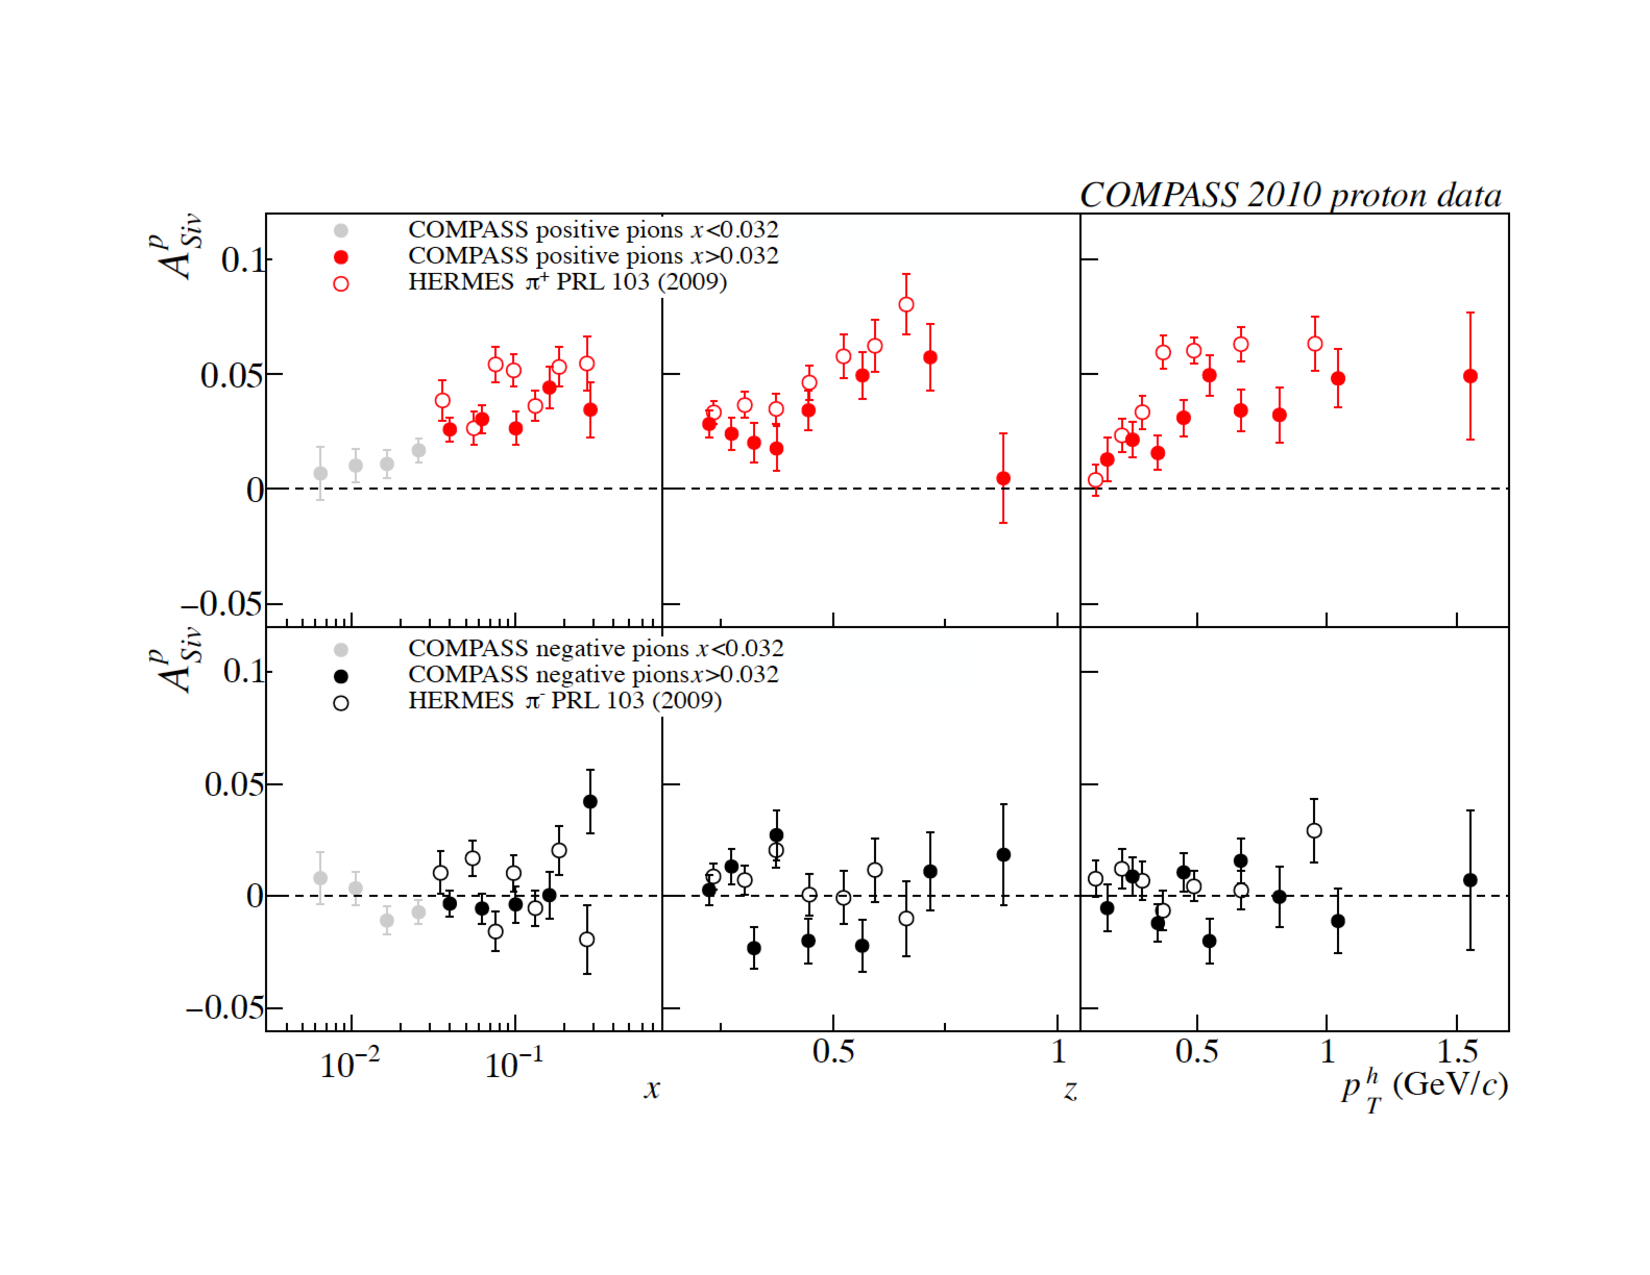
\includegraphics[width=0.6\textwidth, trim=2cm 2cm 2cm
    3cm,clip]{SiversFromSIDIS}
  \caption{The asymmetry amplitude related to the Sivers function measure by
    COMPASS~\cite{Alekseev:2008aa} and HERMES~\cite{Airapetian:2009ae}}
  \label{fig::SiversFromSIDIS}
\end{figure}

The top plot in Fig.~\ref{fig::SiversFromSIDIS} is the asymmetry for a positive
detected hadron.  A positively detected final state hadron is dominated by
u-quark scattering and therefore by the u-quark Sivers function.  This is the
case for three reasons.  Firstly because the SIDIS reaction is weighted by
$e_q^2$ which therefore makes the u-quark scattering four times more likely.
Secondly the so-called favored FF, where the detected hadron is the same charge
as the quark which fragmented, is larger than the unfavored FF.  Therefore a
positively detected hadron most likely resulted from a positively fragmenting
quark.  Thirdly the proton target is composed of twice as many u-quarks as
d-quarks in this scattering kinematic region.  For these three reasons the
results in Fig.~\ref{fig::SiversFromSIDIS} imply that the u-quark Sivers
function from the SIDIS reaction is positive.

The bottom plots in Fig.~\ref{fig::SiversFromSIDIS} suggest that the d-quark
Sivers function in the SIDIS reaction is negative.  The bottom results in
Fig.~\ref{fig::SiversFromSIDIS} are from the combination of u-quark scattering
and fragmenting unfavoredly and d-quark scattering and fragmenting favoredly.
As was mentioned the charge weighting in the SIDIS reaction and the proton quark
composition results in the u-quark scattering with a higher probability.  On the
other hand the previous effect is canceled out by the fact that the favor FF for
the d-quark fragmenting is larger than the unfavored FF for the u-quark
fragmenting.  Therefore the results in the bottom of
Fig.~\ref{fig::SiversFromSIDIS} are for an approximately equal combination from
u-quark scattering and d-quark scattering.  As the u-quark asymmetry amplitude
is positive, the d-quark asymmetry amplitude must therefore be negative and so
also must the d-quark Sivers function.  Anselmino et. al. extracted the Sivers
function using both HERMES and COMPASS data and additional data for
fragmentation functions~\cite{PhysRevD.86.014028}.  These results are shown in
Fig.~\ref{fig::SiversExtractedFromSIDIS}.

\begin{figure}[h!t]
  \centering 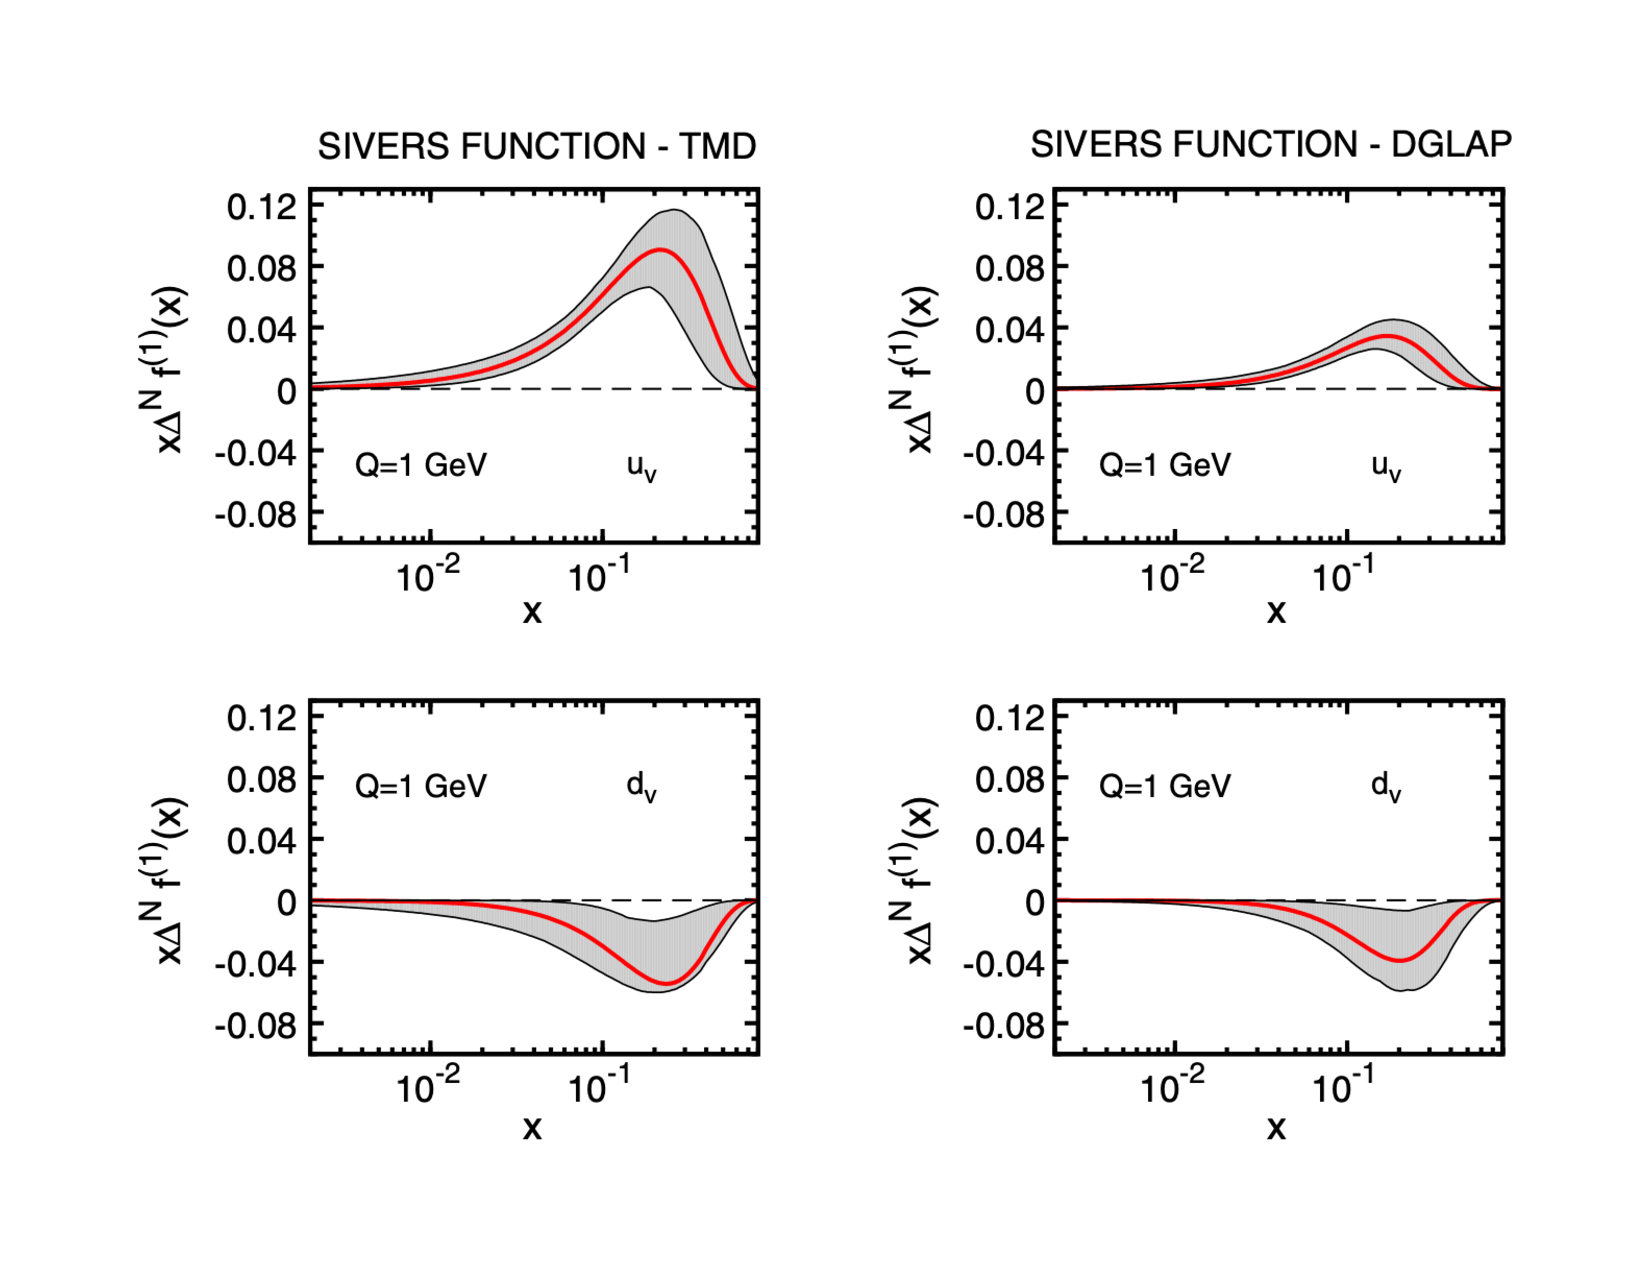
\includegraphics[width=0.6\textwidth, trim=2cm 2cm 2cm 2cm,
    clip]{SiversExtractedFromSIDIS}
  \caption{The valence quark distributions for the first moment of the Sivers
    function.  The left plots are using TMD evolution and the right plots are
    using DGLAP evolution to globally include all measured data.  This image was
    taken from~\cite{PhysRevD.86.014028}}
  \label{fig::SiversExtractedFromSIDIS}
\end{figure}

Results for the TMD asymmetry amplitude, $A_{UU}^{\cos 2\phi_h}$, related to the
Boer-Mulders function were measured by the COMPASS collaboration from
SIDIS~\cite{Adolph:2014pwc}.  As can be seen from the convolution of the
structure function, Eq.~\ref{equ::F_UUcos2phi}, and the definition of asymmetry
amplitudes in SIDIS, Eq.~\ref{equ::asymAmpSIDIS}, this asymmetry amplitude is a
convolution of the Boer-Mulders function and a fragmentation function.  The
COMPASS results for $A_{UU}^{\cos 2\phi_h}$ are shown in
Fig.~\ref{fig::BMFromSIDIS}.  Notably the Boer-Mulders asymmetry amplitude is
higher for negatively scattered hadrons than for positively scattered hadrons
suggesting that the Boer-Mulders function is larger for d-quarks than for
u-quarks.

\begin{figure}[h!t]
  \centering
  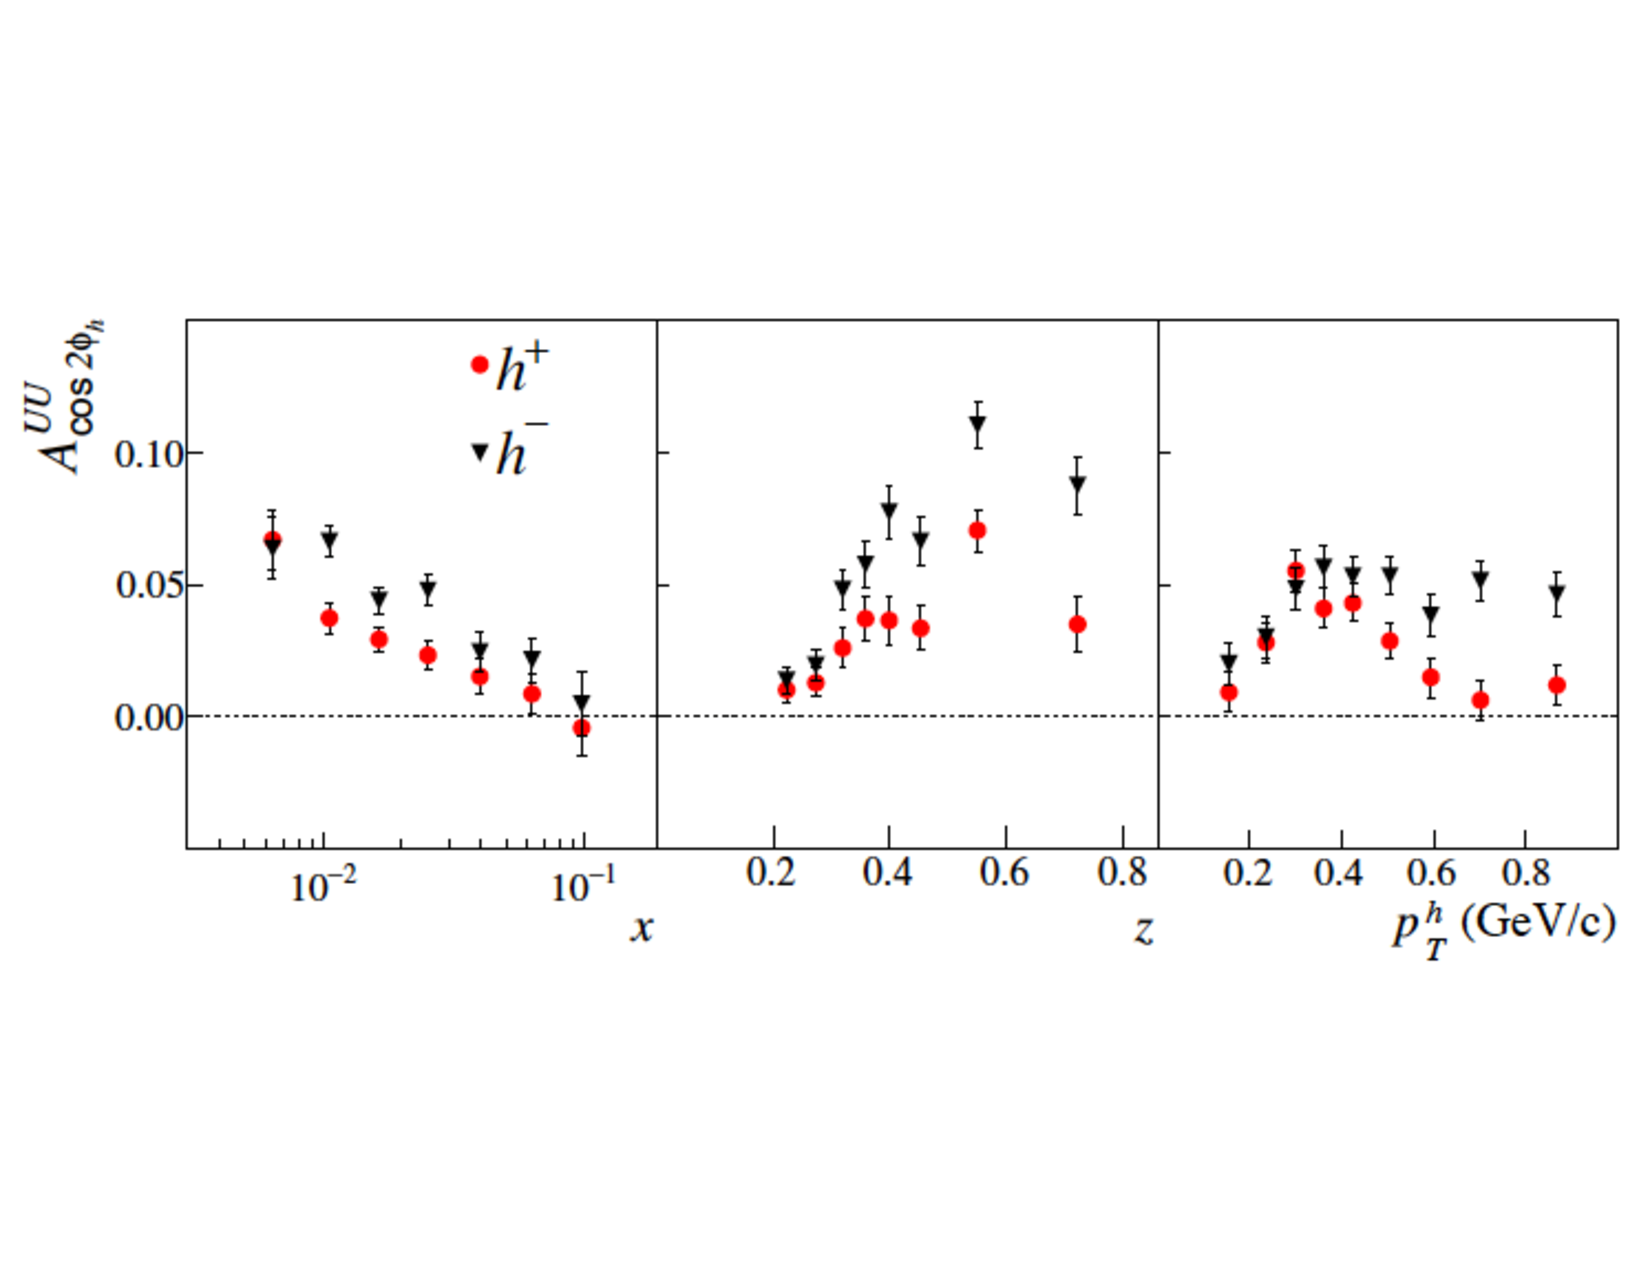
\includegraphics[width=0.7\textwidth,trim=0.3cm 5cm 0cm 4cm,clip]{BMFromSIDIS}
  \caption{COMPASS SIDIS data from muons scattered off of a deuteron target for
    positively scatted hadrons (red) and negatively scattered hadrons (black).
    The asymmetry amplitude is related to the Boer-Mulders functions.  This
    image was taken from~\cite{Adolph:2014pwc}}
  \label{fig::BMFromSIDIS}
\end{figure}

Three SIDIS experiments measured data related to the transversity distribution
from the structure function $F_{UT}^{\sin(\phi_h +\phi_S)}$.  These three
experiments were HERMES~\cite{Airapetian:2004tw,Airapetian:2010ds},
COMPASS~\cite{Ageev:2006da,Alekseev:2008aa,Alekseev:2010rw,Adolph:2012sn,Adolph:2014zba},
and JLab HALL A~\cite{PhysRevLett.107.072003}.  The FF data to determine
$H_1^{\perp }$ from the structure function, $F_{UT}^{\sin(\phi_h +\phi_S)}$,
comes from BELLE~\cite{Abe:2005zx,Seidl:2008xc} and
BABAR~\cite{TheBABAR:2013yha} data in $e^+e^-$ annihilation data.  Anselmino et. al. extracted the transversity distribution~\cite{PhysRevD.87.094019} from
all this data and their results are shown in
Fig.~\ref{fig::transversityExtractedFromSIDIS}.

\begin{figure}[h!t]
  \centering 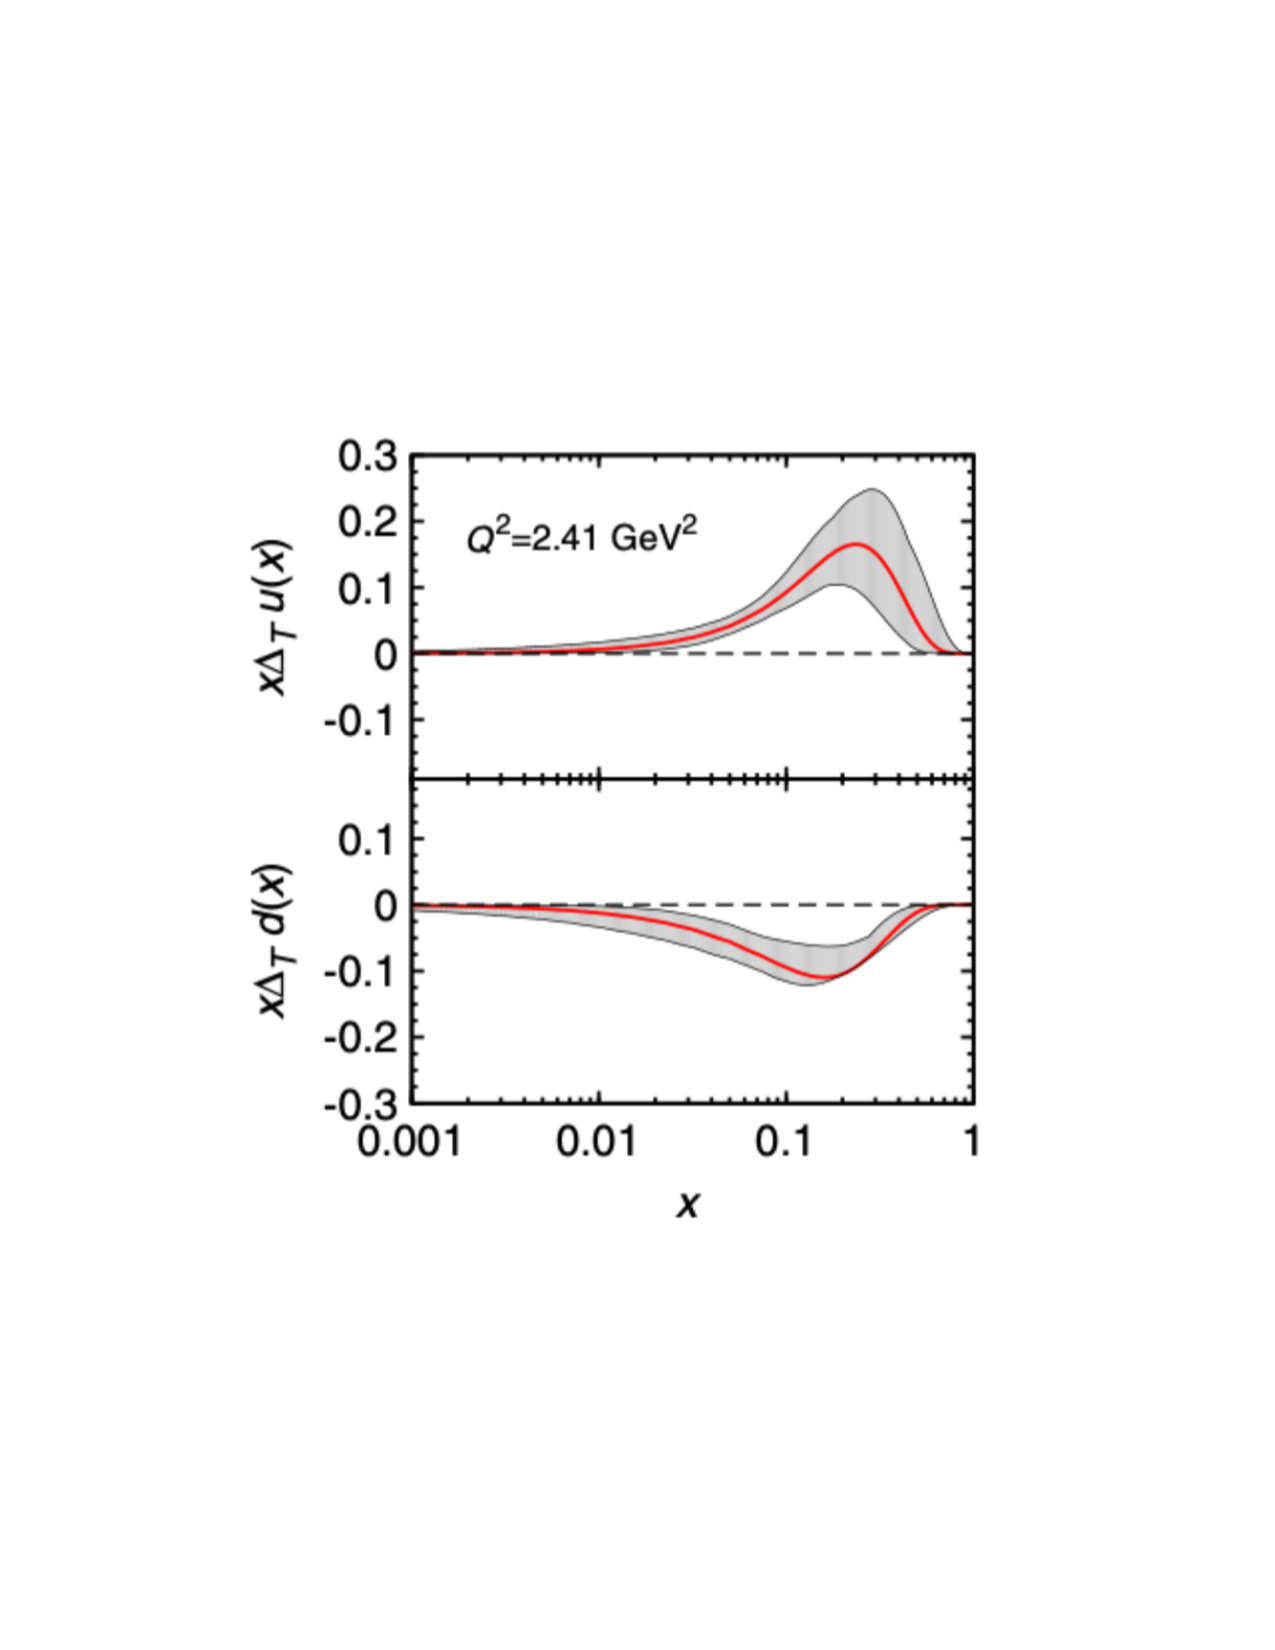
\includegraphics[width=0.4\textwidth, trim=4cm 7cm 4cm 6cm,
    clip]{transversityExtractedFromSIDIS}
  \caption{The transversity distribution for u-quarks (top) and d-quarks
    (bottom) determined from SIDIS data and $e^+e^-$ data.  Image taken
    from~\cite{PhysRevD.87.094019}.}
  \label{fig::transversityExtractedFromSIDIS}
\end{figure}


\section{Drell-Yan} \label{sec::DY}
The Drell-Yan process is the reaction where a quark and an anti-quark annihilate
and the end product results in two detected leptons.  The Drell-Yan process is
denoted as

\begin{equation}
  H_a(P_a) + H_b(P_b, S) \rightarrow \gamma^* + X \rightarrow l(\ell) +
  l'(\ell') + X
\end{equation}
\noindent
where $H_a$ and $H_b$ are hadrons which carry the quark and anti-quarks and in
this thesis only the target hadron, $H_b$ is considered to be polarized with
spin $S$.  In this thesis the quark and anti-quark pair annihilate to form a
virtual photon, $\gamma^*$ and additionally the only final state detected
leptons considered are a muon and an anti-muon pair.  The leading order one
photon exchange diagram is shown in Fig.~\ref{fig::DY_LO}.

\begin{figure}[h!t]
  \centering
  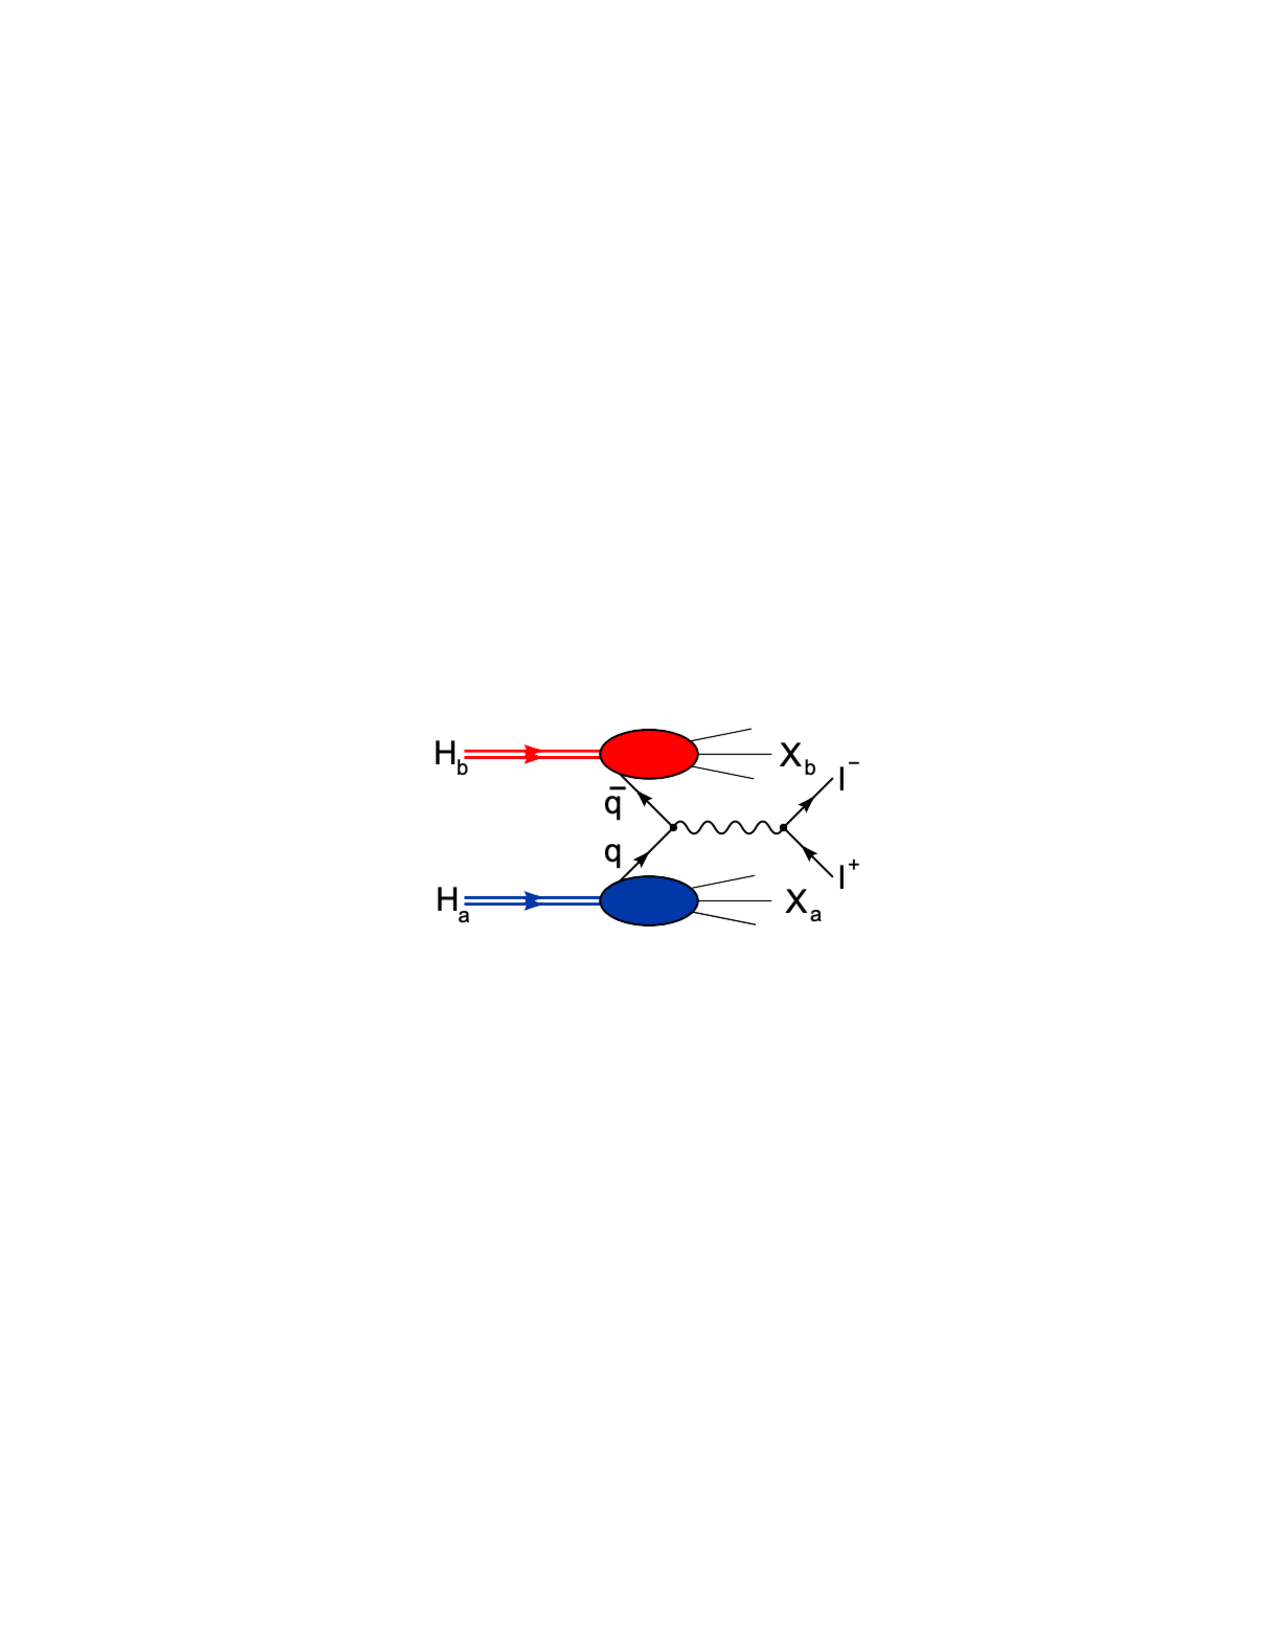
\includegraphics[width=0.45\textwidth, trim=7cm 12cm 7cm 12cm, clip]{DY_LO}
  \caption{The Drell-Yan leading order diagram}
  \label{fig::DY_LO}
\end{figure}

The angles used to define the general Drell-Yan cross-section are defined with
the use of two reference frames.  The target frame (TF),
Fig.~\ref{fig::DY_TargetFrame}, defines the $\phi_S$ angle and the Collins-Soper
(CS), Fig.~\ref{fig::DY_CSFrame}, frame defines the additional $\phi$ and
$\theta$ angles.  The $\phi_S$ angle is defined in the TF as the angle between
the transverse momentum of the virtual photon and the transverse spin of the
target.  The $\phi$ and $\theta$ angles, in the CS frame, are defined as the
azimuthal and polar angle of the negatively charged muon.

\begin{figure}[h!t]
  \centering
  \begin{subfigure}{.46\textwidth}
    \centering
    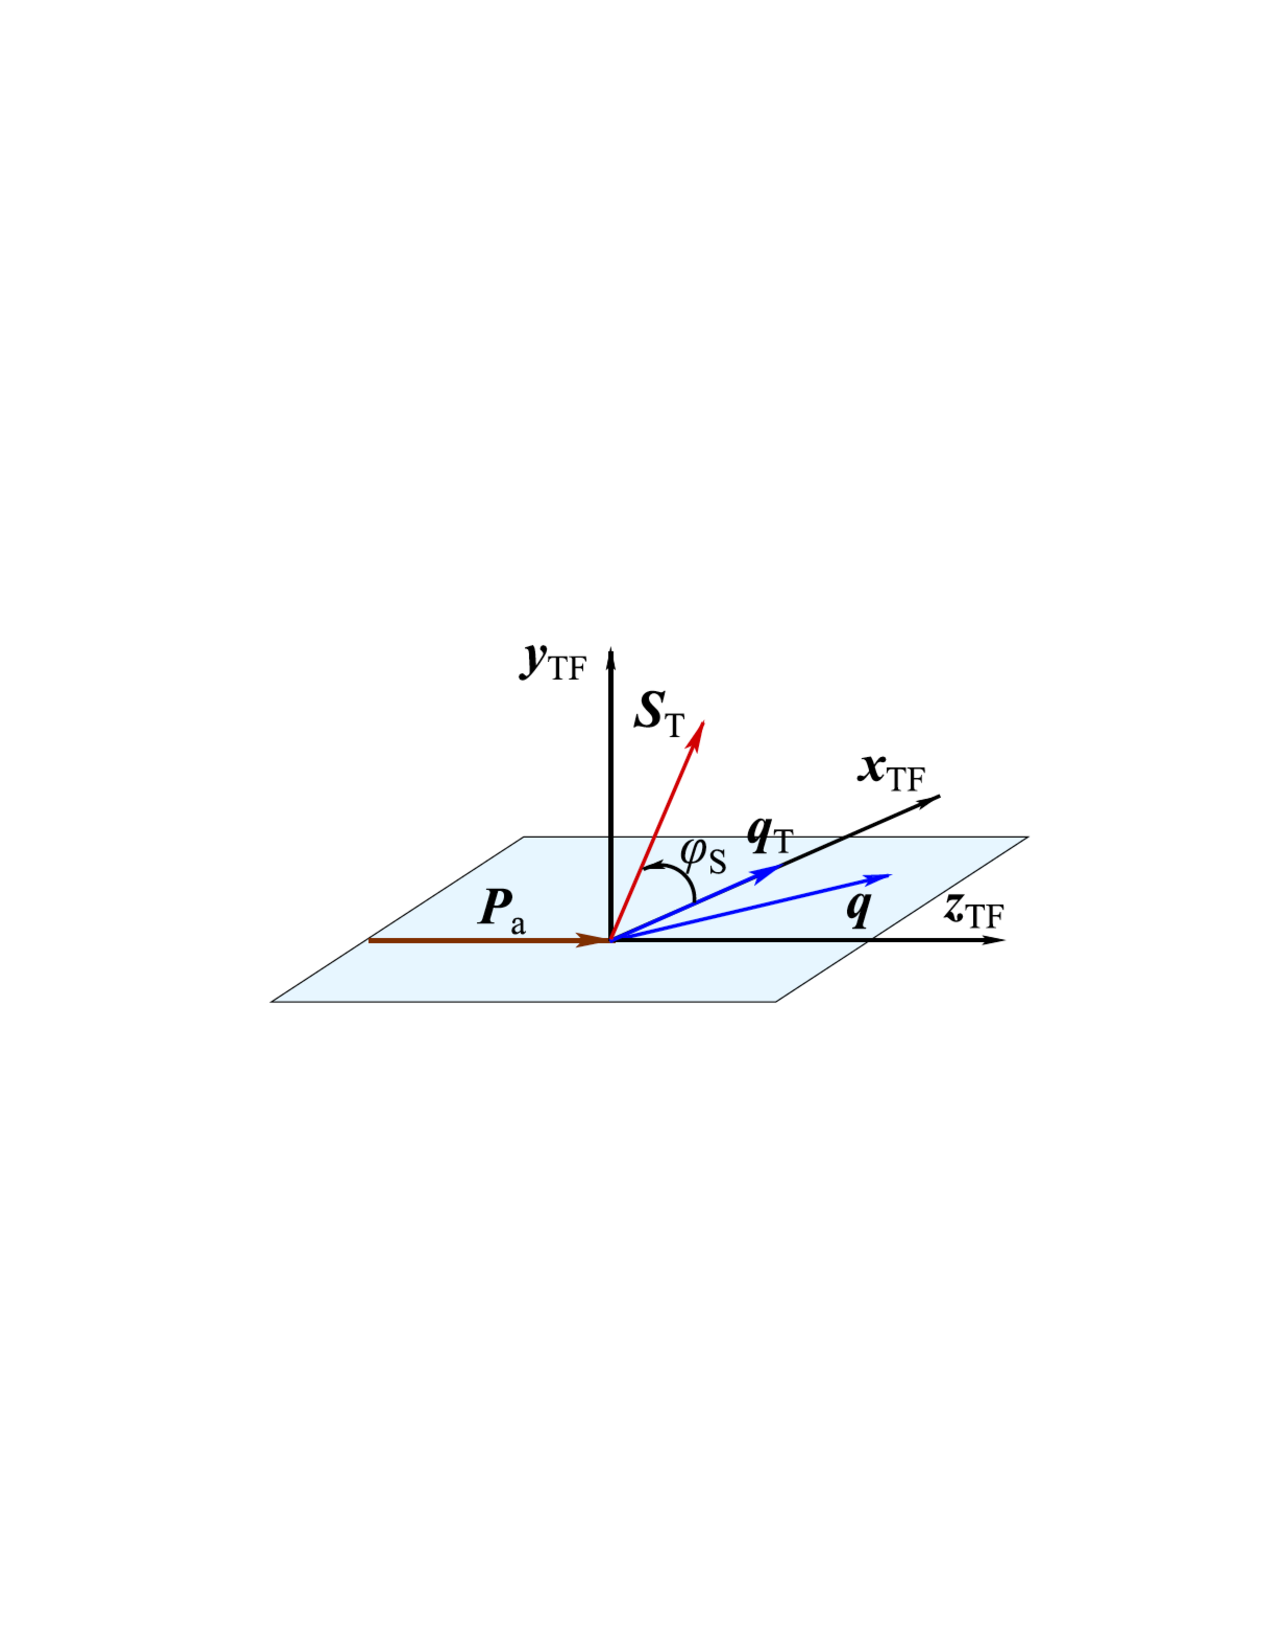
\includegraphics[width=\linewidth, trim=3cm 9cm 3cm 8cm,
      clip]{DY_TargetFrame}
    \caption{The target frame where the z-axis is along the beam and the x-axis
      is in the direction of the transverse momentum of the virtual photon.}
    \label{fig::DY_TargetFrame}%
  \end{subfigure}
  \begin{subfigure}{.02\textwidth}
    \centering
    
\includegraphics[width=\linewidth]{tmp}
    \label{fig::tmp1}%
  \end{subfigure}
  \begin{subfigure}{.46\textwidth}
    \centering
    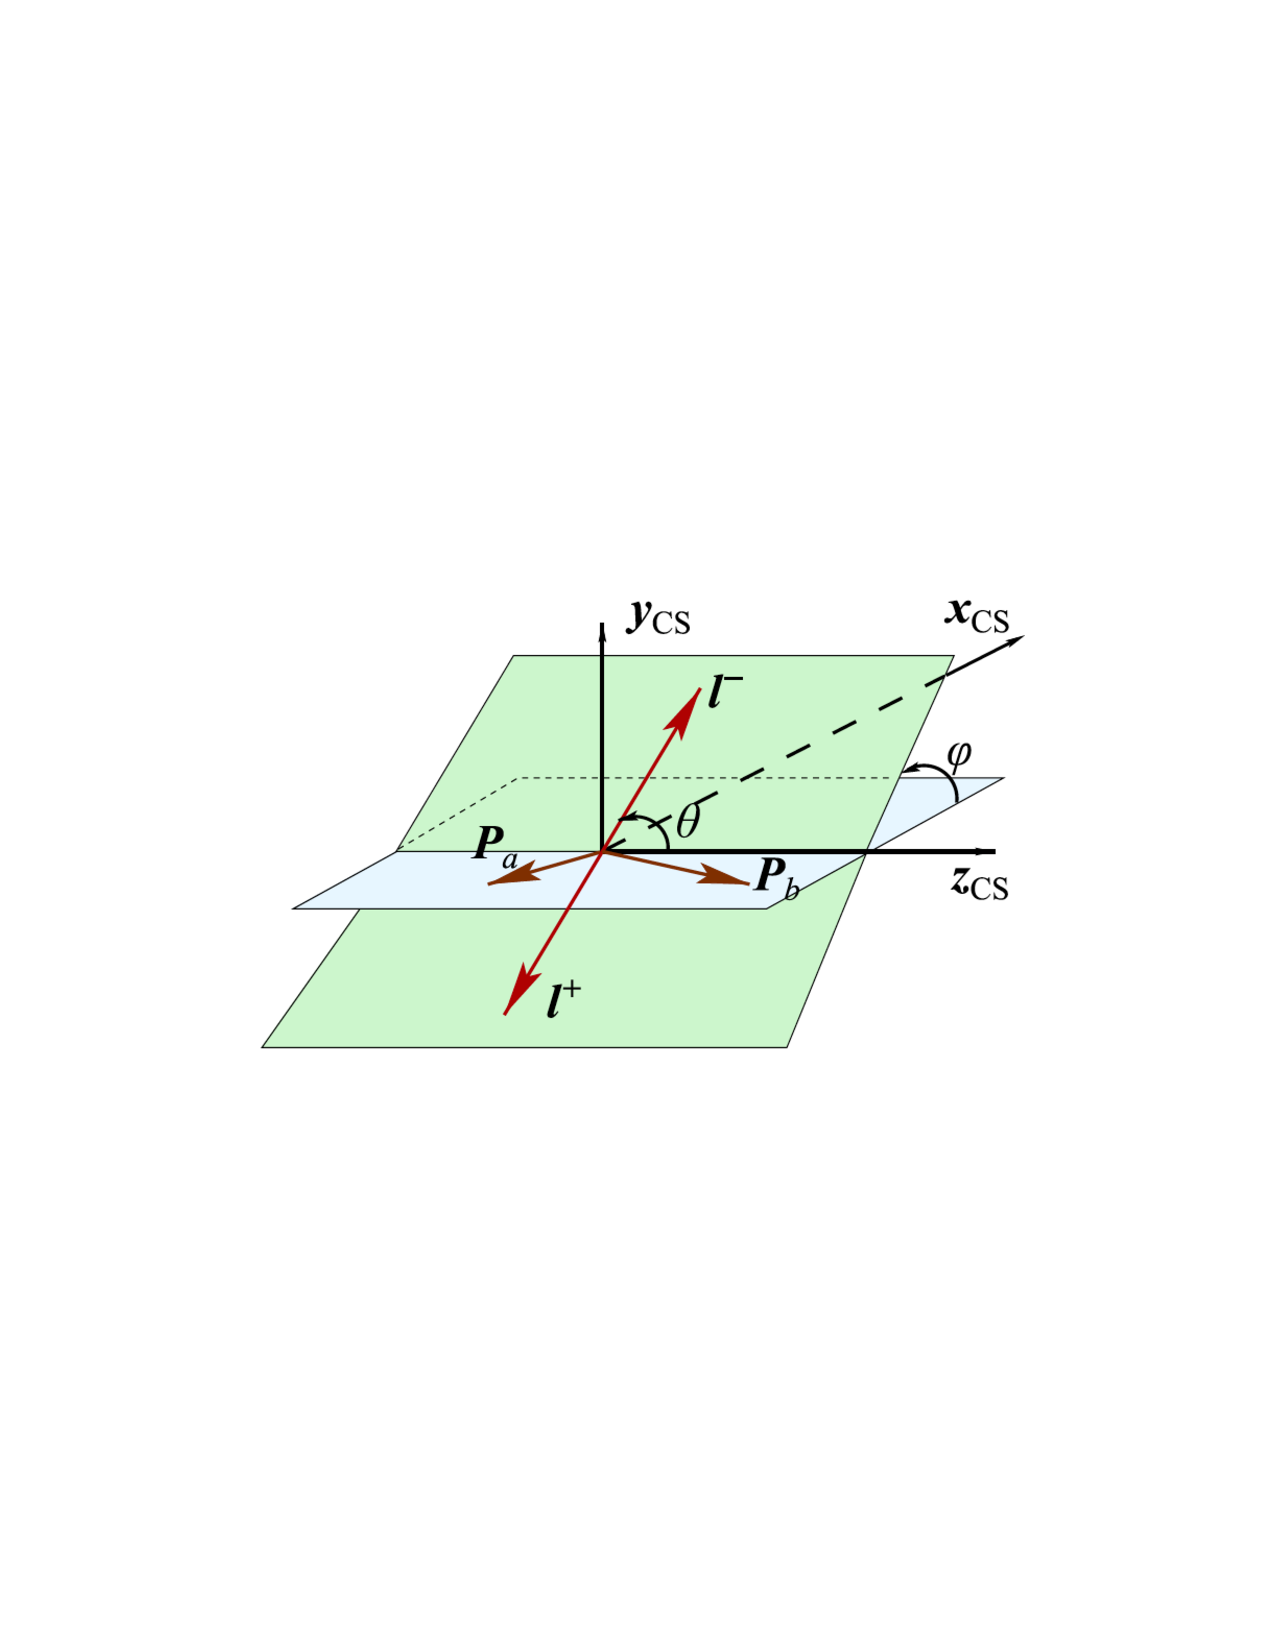
\includegraphics[width=\linewidth, trim=3cm 9cm 3cm 8cm,
      clip]{DY_CSFrame}
    \caption{The Collins-Soper frame is defined in the rest frame of the virtual
      photon where the z-axis bisects the beam and target momentum vectors.}
    \label{fig::DY_CSFrame}%
  \end{subfigure}
\end{figure}

The target frame is defined in the lab frame where the beam is along the z-axis
and the transverse momentum of the virtual photon is along the x-axis.  The
y-axis in the target frame is then chosen so the coordinate system is right
handed.  The Collins-Soper frame is defined in the rest frame of the virtual
photon where the xz-plane coincides with the hadron plane and the z-axis is
chosen so it bisects the momentum vectors $P_a$ and $-P_b$.  The CS frame is
defined from the target frame as a boost first along the along z-axis and then a
boost along the x-axis so the rest frame of the virtual photon is reached.

The leading order model independent Drell-Yan differential cross-section for a
polarized target is~\cite{DYxSection,AKotzininaNote}

\begin{align} \label{equ::DY_ang_dist}
  \frac{d\sigma}{d^4 q \, d \Omega} &=
  \frac{\alpha_{em}^2}{F \, q^2}
  \Big \{ \Big(
   (1 + \cos^2 \theta) \, F_{U}^{1} 
 + (1 - \cos^2 \theta) \, F_{U}^{2} 
 + \sin 2\theta \cos \phi \, F_{U}^{\cos \phi} 
 + \sin^2 \theta \cos 2\phi \, F_{U}^{\cos 2\phi} \Big)
 \nonumber \\
 &+ S_{L} \Big( 
   \sin 2\theta \sin \phi \, F_{L}^{\sin \phi} 
   + \sin^2 \theta \sin 2\phi \, F_{L}^{\sin 2\phi} \Big)
   \nonumber \\
   &+ |S_{T}|
   \Big[ \Big(
     F_{T}^{\sin \phi_S} + \cos^2 \theta \, \tilde{F}_{T}^{\sin \phi_S}
     \Big)\sin \phi_{S} 
     + \Big( F_{T}^{\sin (\phi +\phi_S)} \, \sin(\phi+\phi_S) +
     F_{T}^{(\sin \phi - \phi_S)}\, \sin(\phi-\phi_S) \Big)\sin 2\theta
     \nonumber \\
     & \quad\quad\quad +
     \Big( F_{T}^{\sin (2\phi +\phi_S)}\, \sin(2\phi+\phi_S) +
     F_{T}^{\sin (2\phi - \phi_S)}\, \sin(2\phi-\phi_S) \Big)\sin ^2\theta
     \Big ]
   \Big \},
\end{align}
\noindent
where $F = 4\sqrt{(P_a \cdot P_b)^2 - M_a^2M_b^2}$ is the flux and $\Omega$ is
the solid angle of the outgoing negatively charged muon.  The twelve model
independent structure functions in Eq.~\ref{equ::DY_ang_dist} are labeled as
$F_{Target \; polarization}^{azimuthal \;angle\;coefficient}$.  The phase space
when the TMD regime is valid in DY scattering is when $q_T << q$.  In this
regime the structure functions are equal to a convolution of a beam and a target
TMD function where convolution is defined similarly to the SIDIS case,
Eq.~\ref{equ::SIDIS_conv}, as

\begin{align}
  \label{equ::DY_conv}
  \nonumber
      {\cal C}\bigl[ w(k_{aT}, k_{bT}) f_a \bar{f}_b \bigr] =
      \frac{1}{N_c} \sum_q e_q^2 \int &d^2 k_{aT} d^2 k_{bT} 
      \delta^{(2)}\bigl(q_T - k_{aT} - k_{bT} \bigr) \\
      &\times w(k_{aT},k_{bT})
        \Big[ f_a^q(x,k_{aT}^2)f_b^{\bar{q}}(x,k_{bT}^2) +
          f_a^{\bar{q}}(x,k_{aT}^2)f_b^{q}(x,k_{bT}^2) \Big],
\end{align}
\noindent
where $N_c = 3$ is the number of color charges.  The leading order DY
structure functions in the TMD phase space are related to TMD functions
as~\cite{DYxSection}

\begin{align}
  \label{equ::DY_fU1}
  F_{U}^{1} &  =  
  {\cal C}  \big[ f_{1}  \bar{f}_{1} \big]
  &\propto f^{\bar{u}}_{1,Beam} \otimes f^u_{1,Target}, \\
  \label{equ::DY_fUcos2phi}
  F_{U}^{\cos 2\phi} &  =  
  {\cal C}  \Bigg[ \frac{2\big( \vec{h} \cdot \vec{k}_{aT} \big) 
                          \big( \vec{h} \cdot \vec{k}_{bT} \big)
                         - \vec{k}_{aT} \cdot \vec{k}_{bT}} {M_{a} M_{b}}  
    h_{1}^{\perp}  \bar{h}_{1}^{\perp} \Bigg]
  &\propto h^{\perp \, \bar{u}}_{1,Beam} \otimes h^{\perp \, u}_{1,Target}, \\
F_{L}^{\sin 2\phi} &  =  
-  {\cal C}  \Bigg[ \frac{2\big( \vec{h} \cdot \vec{k}_{aT} \big) 
                          \big( \vec{h} \cdot \vec{k}_{bT} \big)
                         - \vec{k}_{aT} \cdot \vec{k}_{bT}} {M_{a} M_{b}}  
                  h_{1}^{\perp}  \bar{h}_{1L}^{\perp} \Bigg]
&\propto h^{\perp \, \bar{u}}_{1,Beam} \otimes h^{\perp \, u}_{1L,Target}, \\
F_{T}^{1} &  =   
- {\cal C}  \Bigg[ \frac{\vec{h} \cdot \vec{k}_{bT}} {M_{b}}  
  f_{1}  \bar{f}_{1T}^{\perp} \Bigg]
&\propto f^{\bar{u}}_{1,Beam} \otimes f^{\perp \, u}_{1T,Target}, \\
F_{T}^{\sin (2\phi - \phi_S)} &  =  
-  {\cal C}  \Bigg[ \frac{\vec{h} \cdot \vec{k}_{aT}} {M_{a}} 
  h_{1}^{\perp}  \bar{h}_{1} \Bigg]
&\propto h^{\perp \, \bar{u}}_{1,Beam} \otimes h^{u}_{1,Target}, \\
\label{equ::DY_fTsin2phiphiS}
F_{T}^{\sin (2\phi + \phi_S)} &  =  
-  {\cal C}  \Bigg[ \frac{2\big( \vec{h} \cdot \vec{k}_{bT} \big)
                    \big[2 \big( \vec{h} \cdot\vec{k}_{aT} \big)
                         \big( \vec{h} \cdot \vec{k}_{bT} \big)
                        -\vec{k}_{aT} \cdot \vec{k}_{bT} \big]
                   - \vec{k}_{bT}^{2} \big( \vec{h} \cdot \vec{k}_{aT} \big)}
                  {2 M_{a} M_{b}^{2}}  
                  h_{1}^{\perp}  \bar{h}_{1T}^{\perp} \Bigg]
&\propto h^{\perp \, \bar{u}}_{1,Beam} \otimes h^{\perp \, u}_{1T,Target},
\end{align}

\noindent
where $\vec{h} = \vec{q}_T/q_T$ is a unit vector and furthermore the assumption
in this thesis is that the beam $\bar{u}$-quark annihilates with the target
u-quark.  The additional leading order structure functions are zero

\begin{equation}
  F_{U}^{2} \quad = \quad F_{U}^{\cos\phi} \quad = \quad F_{L}^{\sin\phi} \quad
  = \quad F_{T}^{2} \quad = \quad F_{T}^{\sin(\phi - \phi_S)} \quad = \quad
  F_{T}^{\sin(\phi + \phi_S)} \quad = 0.
\end{equation}

The differential cross-seciton, Eq.~\ref{equ::DY_ang_dist}, can be rewritten in
terms of asymmetry amplitudes and depolarization factors.  The asymmetry
amplitudes are defined similarly to the case in SIDIS,
Eq.~\ref{equ::asymAmpSIDIS}, and again for the reason that asymmetries can be
determined to a higher precision than structure functions.  For Drell-Yan these
asymmetry amplitudes are

\begin{equation}
  A^{w_i(\phi, \phi_S)}_{Target} = \frac{F^{w_i(\phi,
      \phi_S)}_{Target}}{F_{U}^1+F_{U}^2}.
  \label{equ::asymAmpDY}
\end{equation}
\noindent
The asymmetry amplitudes are the result of different virtual photon
polarizations decaying to a final state lepton pair.  The depolarization factor
is defined as the ratio of the virtual photon polarization to produce such an
asymmetry to that of a transversely polarized virtual photon.  The
depolarization is defined for each asymmetry amplitude as

\begin{equation}
  D_{[f(\theta)]} = \frac{f(\theta)}{1+A_U^1\;\cos^2\theta},
  \label{equ::DYDepolarizationFactorDef}
\end{equation}
\noindent
where the function $f(\theta)$ corresponds to virtual photon angular decay
responsible for the given asymmetry.  The Drell-Yan differential cross-section,
Eq.~\ref{equ::DY_ang_dist}, now simplifies to~\cite{AKotzininaNote}

\begin{align}
  \label{equ::DY_usefulXsect}
  \frac{d\sigma}{d^4 q \, d \Omega} &=
  \frac{\alpha_{em}^2}{F \, q^2}\hat{\sigma}_U
  \Big \{ \Big(1 + D_{[\sin^2 \theta]} \cos 2\phi \, A_{U}^{\cos 2\phi} \Big)
 \nonumber \\
 &+ S_{L} D_{[\sin^2 \theta]} \sin 2\phi \, A_{L}^{\sin 2\phi}
   \nonumber \\
   &+ |S_{T}|
   \Big[A_{T}^{\sin \phi_S}\;\sin \phi_{S} 
     + \Big( A_{T}^{\sin (2\phi +\phi_S)}\, \sin(2\phi+\phi_S) +
     A_{T}^{\sin (2\phi - \phi_S)}\, \sin(2\phi-\phi_S) \Big)D_{[\sin ^2\theta]}
     \Big ]
   \Big \},
\end{align}
\noindent
where $\hat{\sigma}_U = F^1_U (1+\cos^2\theta)$ is the unpolarized DY
cross-section.  For the data taking conditions in 2015 it is assumed that the target is transversely polarized so $S_L = 0$ and therefore the Drell-Yan cross-section can be simplified to

\begin{align}
  \label{equ::DY_MostusefulXsect}
  \frac{d\sigma}{d^4 q \, d \Omega} &=
  \frac{\alpha_{em}^2}{F \, q^2}\hat{\sigma}_U
  \Big \{ \Big(1 + D_{[\sin^2 \theta]} \cos 2\phi \, A_{U}^{\cos 2\phi} \Big)
   \nonumber \\
   &+ |S_{T}|
   \Big[A_{T}^{\sin \phi_S}\;\sin \phi_{S} 
     + \Big( A_{T}^{\sin (2\phi +\phi_S)}\, \sin(2\phi+\phi_S) +
     A_{T}^{\sin (2\phi - \phi_S)}\, \sin(2\phi-\phi_S) \Big)D_{[\sin ^2\theta]}
     \Big ]
   \Big \}.
\end{align}

\subsection{Drell-Yan Sivers Result}
The first Drell-Yan results for the Sivers asymmetry amplitude, in an attempt to
verify the sign change between Drell-Yan and SIDIS, came from hadron-hadron
collisions at Star~\cite{PhysRevLett.116.132301}.  Their result measured the
Sivers amplitude from $pp^{\uparrow} \rightarrow Z^0X$ and $pp^{\uparrow}
\rightarrow W^{\pm}X$ and are shown in Fig.~\ref{fig::StarSivers}.  The
statistical error bars are too high and the $Q^2$ scale is very different from
that used to measure a Sivers function in SIDIS however.  As of the data of this
thesis it is impossible to conclude on a sign change of the Sivers function
between Drell-Yan and SIDIS.

\begin{figure}[h!t]
  \centering
  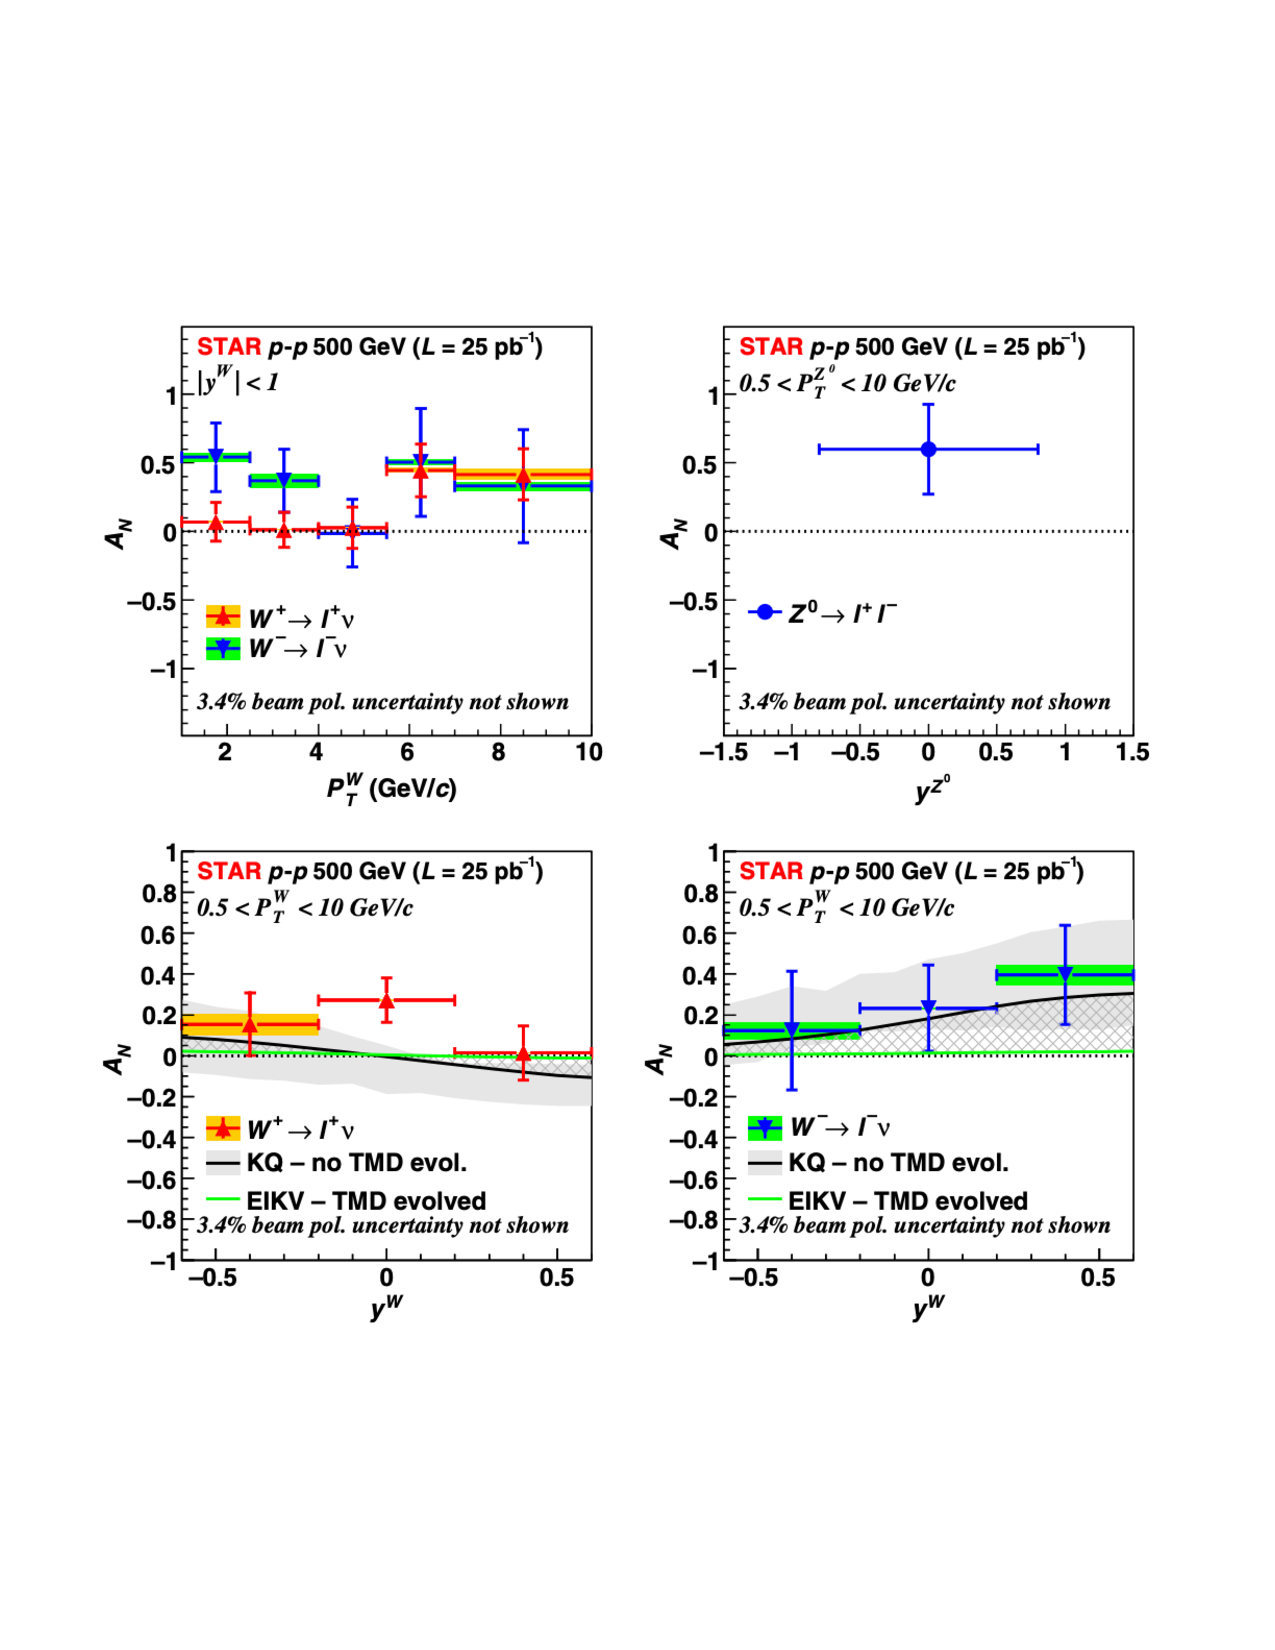
\includegraphics[width=0.7\textwidth, trim=1cm 5cm 1cm 5cm]{StarSivers}
  \caption{All plots show a left-right asymmetry which is related to the Sivers
    function.  The top right plot is for $Z^0$ production while the other three
    plots are for $W^\pm$ production.  $Q^2$ evolution and resulting error bars
    from EIKV~\cite{PhysRevD.89.074013} and KQ~\cite{PhysRevLett.103.172001}.
    Image taken from~\cite{PhysRevLett.116.132301}.}
  \label{fig::StarSivers}
\end{figure}

\subsection{Left-Right Asymmetry} \label{sec::lr_theory}
An asymmetry of interest for measuring high energy spin related phenomena is the
analyzing power.  This asymmetry is denoted $A_N$ and is responsible for a
left-right asymmetry for a suitable definition of left and right.  The
cross-section for spin 1/2 particles scattering where one of the initial
particles is polarized can be written

\begin{equation}
  \label{equ::AN_xsect}
  I(\theta, \phi) = I_0(\theta)(1+SA_N \cos(\phi))
\end{equation}
\noindent
where $I_0$ is the unpolarized cross-section, $S$ is the beam or target
polarization percentage and $\phi$ is the azimuthal scattering angle of the
outgoing measured particle.  Working in the target frame for Drell-Yan
scattering from a transversely polarized target, the azimuthal angle can be
redefined in terms of the $\phi_S$ angle by noting that $\phi = \frac{\pi}{2} -
\phi_S$. Eq.~\ref{equ::AN_xsect} can then be written in the form of the
Drell-Yan cross-section, Eq.~\ref{equ::DY_usefulXsect}, as

\begin{align}
  \frac{d\sigma}{d^4 q \, d \phi_S} &= \frac{\alpha_{em}^2}{F \,
    q^2}\hat{\sigma}_U\Big(1+|S_T|A_N \cos (\frac{\pi}{2} - \phi_S) \Big)
  \\ \nonumber
  &= \frac{\alpha_{em}^2}{F \,
    q^2}\hat{\sigma}_U\Big(1+|S_T|A_N \sin(\phi_S) \Big)
  \\ \nonumber
  &= \frac{\alpha_{em}^2}{F \,
    q^2}\hat{\sigma}_U \Big(1+|S_T| A_{T}^{\sin \phi_S} \sin(\phi_S)\Big),
\end{align}
\noindent
where this relation is obtained from Eq.~\ref{equ::DY_usefulXsect} by
integrating over all angle except $\phi_S$ and where the polarization $S$ is
assumed to be transverse.  Therefore the analyzing power, $A_N$, is the same as
the Sivers asymmetry amplitude, $A_{T}^{\sin \phi_S}$, for Drell-Yan scattering.

An analysis technique for measuring $A_N$ is by making a left-right asymmetry.
The left-right asymmetry is defined as 
\begin{equation}
  A_{lr} = \frac{1}{|S_T|}\frac{\sigma_l - \sigma_r}{\sigma_l + \sigma_r},
\end{equation}
\noindent
where $\sigma_{l(r)}$ is the cross-section for producing a final state to
the left(right).  In the target frame the definition of left scattering is
$\int_{\phi_S=0}^{\phi_S=\pi}\frac{d\sigma}{d^4 q \, d \phi_S} d\phi_S$ and
definition of right scattering is
$\int_{\phi_S=\pi}^{\phi_S=2\pi}\frac{d\sigma}{d^4 q \, d \phi_S} d\phi_S$.  It
is straight forward to show the relationship between $A_{lr}$ and $A_N$ as

\begin{align}
  A_{lr} &= \frac{1}{|S_T|}
  \frac{\int_{\phi_S=0}^{\phi_S=\pi} \frac{d\sigma}{d^4 q \, d \phi_S}d\phi_S
    - \int_{\phi_S=\pi}^{\phi_S=2\pi}\frac{d\sigma}{d^4 q \, d \phi_S}d\phi_S}
       {\int_{\phi_S=0}^{\phi_S=\pi}\frac{d\sigma}{d^4 q \, d \phi_S}d\phi_S
         + \int_{\phi_S=\pi}^{\phi_S=2\pi}\frac{d\sigma}{d^4 q \, d \phi_S}d\phi_S}
       \\ \nonumber
       &= \frac{1}{|S_T|}
       \frac{\phi_S -|S_T|A_N\cos\phi_S \Big|_0^{\pi}
       - \Big(\phi_S -|S_T|A_N\cos\phi_S \Big)\Big|_{\pi}^{2\pi}}
            {\phi_S -|S_T|A_N\cos\phi_S \Big|_0^{\pi}
              + \Big(\phi_S -|S_T|A_N\cos\phi_S \Big)\Big|_{\pi}^{2\pi}}
            \\ \nonumber
            &= \frac{1}{|S_T|}
            \frac{4|S_T|A_N}{2\pi}
            \\ \nonumber
            &= \frac{2A_N}{\pi}.
\end{align}

Another method to determine $A_N$, is with the transverse spin asymmetry (TSA)
defined as
\begin{align}
  \label{equ::AN_TSA}
  A_{TSA} =& \frac{1}{|S_T|} \frac{\frac{d\sigma^{\uparrow}}{d\phi_s} -
    \frac{d\sigma^{\downarrow}}{d\phi_s}} {\frac{d\sigma^{\uparrow}}{d\phi_s} +
    \frac{d\sigma^{\downarrow}}{d\phi_s}} \\ \nonumber =& \frac{1}{|S_T|} \frac{1 +
    |S_T|A_N\sin\phi_S - \Big(1 + |S_T|A_N\sin(\phi_S + \pi) \Big)} {1 + |S_T|A_N\sin\phi_S
    + \Big(1 + |S_T|A_N\sin(\phi_S + \pi) \Big)} \\ \nonumber =& A_N\sin\phi_S.
\end{align}

To understand how $A_N$ is related to the Sivers function, it is illustrative to
write the Drell-Yan differential cross-section under the TMD assumptions
as~\cite{PhysRevLett.103.172001}
\begin{equation}
  \frac{d\sigma^{H_aH_b\rightarrow l^+l^- X}}{d\eta dM^2d^2q_T} =
  \hat{\sigma}_0 \sum_q e^2_q \int d^2k_{aT} d^2k_{bT}
  \delta^{(2)}(k_{aT}+k_{bT}-q_T)
  f_{\bar{q}/H_a}(x_a, k_{aT})f_{q/H_b}(x_b, k_{bT}),
\end{equation}
\noindent
 $\eta$ is rapidity and $f_{\bar{q}(q)/H_{a(b)}}$ is a TMD function.  Inserting
this cross-section into the transverse spin asymmetry, Eq.~\ref{equ::AN_TSA},
and using proper TMD functions for the given transverse polarization gives
\begin{align}
  A_{TSA} &= A_N \sin \phi_S
  \\ \nonumber
  &= -\frac{1}{S}
  \frac{\sum_q e^2_q \int d^2k_{aT} d^2k_{bT}
    \delta^{(2)}(k_{aT}+k_{bT}-q_T)f_{\bar{q}/H_a}(x_a, k_{aT})
    \frac{k_{bT}}{M_b}f_{1T}^{\perp q}(x_b, k_{bT})
    S\sin \phi_S}
  {\sum_q e^2_q \int d^2k_{aT} d^2k_{bT}
    \delta^{(2)}(k_{aT}+k_{bT}-q_T)
    f_{\bar{q}/H_a}(x_a, k_{aT})f_{q/H_b}(x_b, k_{bT})}.
\end{align}

Several experiments measured large values for $A_N$ at different center of mass
energies.  Fig.~\ref{fig::AN_vsXF} shows the results of $A_N$ from hadron-hadron
collisions from four different experiments over a range of center of mass
energies.

\begin{figure}[h!t]
  \centering
  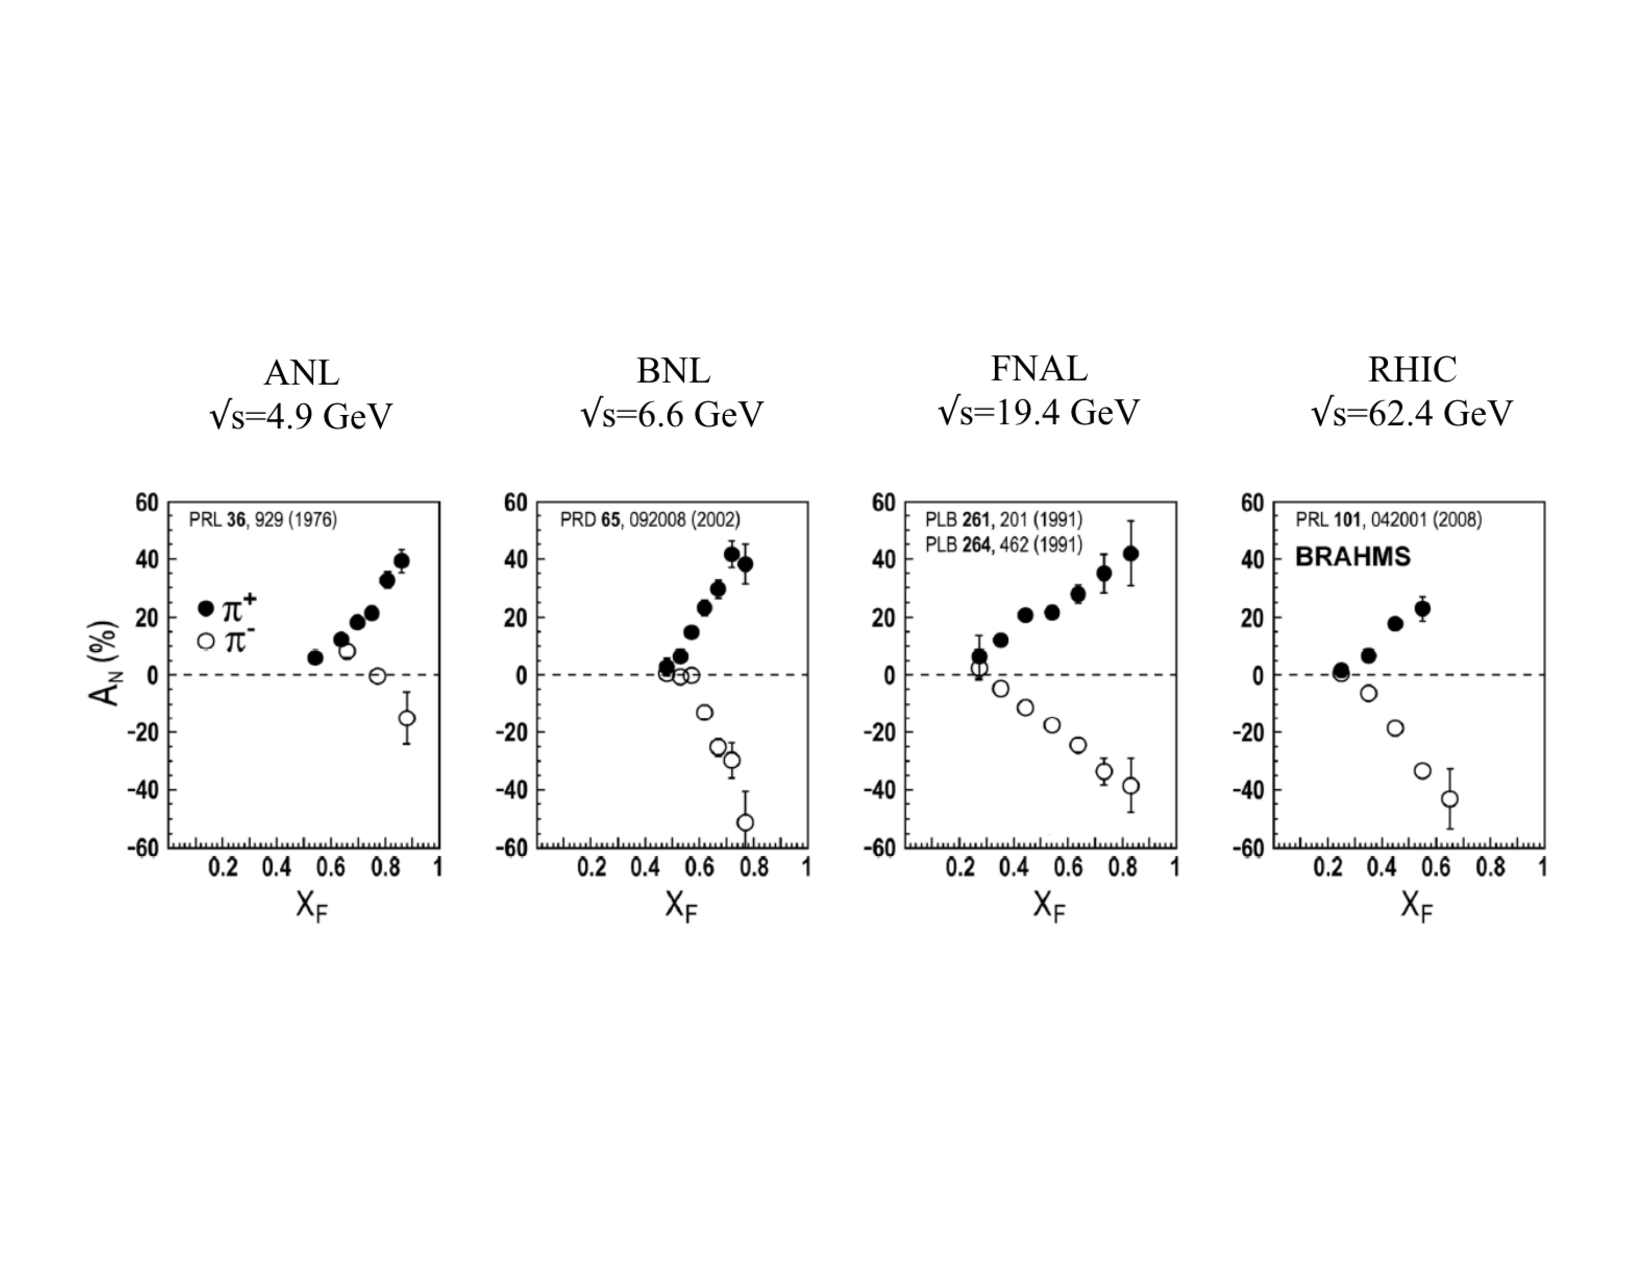
\includegraphics[width=0.9\textwidth, trim=1cm 6cm 1cm 6cm, clip]{AN_vsXF}
  \caption{Large $A_N$ values where found at ANL~\cite{PhysRevLett.36.929},
    BNL~\cite{PhysRevD.65.092008}, FNAL~\cite{ADAMS1991201,ADAMS1991462} and
    RHIC~\cite{PhysRevLett.101.042001}.}
  \label{fig::AN_vsXF}
\end{figure}

\subsection{Weighted Asymmetries from Drell-Yan}\label{sec::qt_w_theory}

The proton TMD functions, determined from Drell-Yan in
Eqs.~\ref{equ::DY_fU1}-\ref{equ::DY_fTsin2phiphiS}, are convoluted with a TMD
function from the beam pion.  The Drell-Yan convolution, Eq.~\ref{equ::DY_conv},
makes it difficult to determine a single TMD function and for this reason model
assumptions are made in the global analysis to extract the individual TMDs from
the convolutions.  An alternative method involving weighted asymmetries however,
makes it possible to disentangle the convolution and determine a $k_T^2$ moment
of a TMD function both for
SIDIS~\cite{Kotzinian:1995cz,Kotzinian:1997wt,Boer:1997nt} and for
Drell-Yan~\cite{Efremov:2004tp,Sissakian:2005vd,Sissakian:2005yp,Wang:2017onm}.

The deconvolution by weighted asymmetries works by multiplying a given structure
function by an appropriate weight and integrating over the virtual photon
transverse momentum, $q_T$.  The simplest Drell-Yan structure function to
deconvolute is $F_U^1$.  By integrating Eq.~\ref{equ::DY_fU1} over $q_T$ the
convolution equation becomes

\begin{align}
  \label{equ::DY_fu1_qtint}
  \int d^2{q_T} F_U^1 &=
  \int d^2{q_T} {\cal C}  \big[ f_{1,a} \bar{f}_{1,b} \big]
  \\ \nonumber
  &= \int d^2{q_T} \frac{1}{N_c} \sum_q e_q^2 \int d^2 k_{aT} d^2 k_{bT} 
  \delta^{(2)}\bigl(q_T - k_{aT} - k_{bT} \bigr)
  \\ \nonumber
  & \quad\quad\quad
  \times \Big[ f_{1,a}^q(x_a,k_{aT}^2)f_{1,b}^{\bar{q}}(x_b,k_{bT}^2) +
    f_{1,a}^{\bar{q}}(x_a,k_{aT}^2)f_{1,b}^{q}(x_b,k_{bT}^2) \Big]
  \\ \nonumber
  &= \frac{1}{N_c} \sum_q
  e_q^2 f_{1,a}^q(x_a)f_{1,b}^{\bar{q}}(x_b) +
  f_{1,a}^{\bar{q}}(x_a)f_{1,b}^{q}(x_b)
  \\ \nonumber
   \substack{COMPASS \\ \approx} \quad &
   \frac{4}{27}f_{1,\pi}^{\bar{u}}(x_\pi)f_{1,proton}^u(x_{proton}),
\end{align}

\noindent
where $f_1(x) = \int d^2 k_{T} f_1(x,k_{T}^2)$ is a TMD function integrated over
$k_T$.  In Eq.~\ref{equ::DY_fu1_qtint} the weight was 1 and no assumptions were
needed to perform the integration.  The answer is a TMD function for the beam
multiplied by a TMD function from the target.  The final equality in
Eq.~\ref{equ::DY_fu1_qtint} is valid in the COMPASS kinematic region and shows
how straight forward this method can make TMD extraction.

Deconvoluting the additional Drell-Yan structure functions,
Eqs~\ref{equ::DY_fUcos2phi}-\ref{equ::DY_fTsin2phiphiS}, is similar to
Eq.~\ref{equ::DY_fu1_qtint} but requires a different weight.  The Sivers TMD
function can be extracted from the $F_T^1$ structure function using a weight
equal to $|q_T|/M_b$.  This can be seen by multiplying $F_T^1$ by the weight
$|q_T|/M_b$, and integrating over $q_T$ to remove the Dirac delta function as
follows

\begin{align}
  \label{equ::DY_ft_qtint}
  \int d^2{q_T} \frac{|q_T|}{M_b} F_T^1 &=
  - \int d^2{q_T} \frac{|q_T|}{M_b} {\cal C}
  \Big[\frac{\vec{q}_T \cdot \vec{k}_{bT}} {|q_T|M_{b}}  
  f_{1,a}  \bar{f}_{1T,b}^{\perp} \Big]
  \\ \nonumber
  &= - \int d^2{q_T} \frac{|q_T|}{M_b}
  \frac{1}{N_c} \sum_q e_q^2 \int d^2 k_{aT} d^2 k_{bT} 
  \delta^{(2)}\bigl(q_T - k_{aT} - k_{bT} \bigr)
  \\ \nonumber
  & \quad\quad\quad
  \times \frac{\vec{q}_T \cdot \vec{k}_{bT}} {|q_T|M_{b}}
  \Big[ f_{1,a}^q(x_a,k_{aT}^2)f_{1T,b}^{\bar{q}\perp}(x_b,k_{bT}^2) +
    f_{1,a}^{\bar{q}}(x_a,k_{aT}^2)f_{1T,b}^{q\perp}(x_b,k_{bT}^2) \Big]
  \\ \nonumber
  &= - \frac{1}{N_c} \sum_q e_q^2 \int d^2 k_{aT} d^2 k_{bT} 
  \times \frac{(\vec{k}_{aT} + \vec{k}_{bT}) \cdot \vec{k}_{bT}} {M^2_{b}}
  \Big[ f_{1,a}^q(x_a,k_{aT}^2)f_{1T,b}^{\bar{q}\perp}(x_b,k_{bT}^2) +
    f_{1,a}^{\bar{q}}(x_a,k_{aT}^2)f_{1T,b}^{q\perp}(x_b,k_{bT}^2) \Big].
\end{align}
\noindent
To simplify further we make use of the fact that the unpolarized quark
distribution function is even in $k_T$ which means
\begin{equation}
  \int_{-\infty}^{\infty} d^2 k_{aT} \vec{k}_{aT} \cdot \vec{k}_{bT}
  f_{1,a}(x_a, k_{aT}^2) = 0,
\end{equation}
\noindent
and therefore only even terms in $k_T^2$ need to be
considered. Eq.~\ref{equ::DY_ft_qtint} can then be further simplified as

\begin{align}
  \int d^2{q_T} \frac{|q_T|}{M_b} F_T^1 &=
  - \frac{2}{N_c} \sum_q e_q^2
  \Big[ f_{1,a}^q(x_a) f_{1T,b}^{(1)\bar{q}\perp}(x_b) +
    f_{1,a}^{\bar{q}}(x_a) f_{1T,b}^{(1)q\perp}(x_b) \Big]
  \\ \nonumber
  \substack{COMPASS \\ \approx}& \quad
  - \frac{8}{27}
  f_{1,\pi}^{\bar{u}}(x_\pi)f_{1T,proton}^{(1)u\perp}(x_{proton}),
\end{align}
\noindent
where the $f_{1T}^{(1)q\perp}(x) = \int d^2 k_{T}
\frac{k_T^2}{2M}f_{1T}^{q\perp}(x, k_T^2)$ is the first $k_T^2$ moment of the
Sivers function and the general $k_T$ moment of a TMD is defined as $f^{(n)}(x)
= \int d^2 k_{T} \Big(\frac{k_T^2}{2M}\Big)^nf(x, k_T^2)$.

The essential steps in deconvolution the TMD functions are to multiply by a
weight which gets rid of any ${q_T}$ terms outside of the Dirac delta function
and to only include even terms in $k_T$.  The remaining two transverse
spin-dependent structure functions can also be deconvoluted in a similar fashion
to give

\begin{align}
  \label{equ::DY_fpretz_qtint}
  \int d^2{q_T} \frac{|q_T|^3}{2M_aM_b^2} F_T^{\sin(2\phi+\phi_S)} &=
  - \frac{2}{N_c} \sum_q e_q^2 \Big[
    h_{1,a}^{(1)\bar{q}\perp}(x_a)h_{1T,b}^{(2)q\perp}(x_b) +
    (q\leftrightarrow\bar{q})
    \Big]
  \\ \nonumber
  \substack{COMPASS \\ \approx} & \;
  - \frac{8}{27} h_{1,\pi}^{(1)\bar{u}\perp}(x_{\pi})\;
  h_{1T,proton}^{(2)u\perp}(x_{proton}),
  \\ \nonumber
  \\
  \label{equ::DY_ftrans_qtint}
  \int d^2{q_T} \frac{|q_T|}{M_a} F_T^{\sin(2\phi-\phi_S)} &=
  - \frac{2}{N_c} \sum_q e_q^2 \Big[
    h_{1,a}^{(1)\bar{q}\perp}(x_a)h_{1,b}^{(2)q}(x_b) +
    (q\leftrightarrow\bar{q})
    \Big]
  \\ \nonumber
  \substack{COMPASS \\ \approx} & \;
  - \frac{8}{27} h_{1,\pi}^{(1)\bar{u}\perp}(x_{\pi})\;
  h_{1,proton}^{(2)u}(x_{proton}),
\end{align}
\noindent
where Eq.~\ref{equ::DY_fpretz_qtint} can be used to determined the proton
pretzelosity function and Eq.~\ref{equ::DY_ftrans_qtint} can be used to
determine the proton transversity function.

For experimentally determining the $k_T^2$ moments of TMD functions the
following weighted asymmetries amplitudes are defined

\begin{equation}
  A^{YW_Y}{X}(x_a, x_b) = \frac{\int d^2{q_T} W_YF^Y_X}{\int d^2{q_T} F_U^1},
\end{equation}
\noindent
where $Y$ is the azimuthal modulation of interest, $W_Y$ is the appropriate
weight and $X$ denotes the targets polarization.  For example the Sivers
weighted asymmetry amplitude is as follows

\begin{equation}
  A^{\sin \phi_S \frac{q_T}{M_b}} =
  \frac{\int d^2{q_T} \frac{q_T}{M_b}F^{\sin \phi_S}_T}{\int d^2{q_T} F_U^1}
  \quad\quad \substack{COMPASS \\ \approx} \;
  -2\frac{f_{1T,proton}^{(1)u\perp}(x_{proton})}{f_{1,proton}}.
\end{equation}

\subsection{J/$\Psi$ Production}\label{sec::theory_jpsi}
The production of J/$\Psi$ hadrons potentially offers an alternative mechanism
for studying TMD related effects.  As of yet however, there is no confirmation
on the J/$\Psi$ production mechanism and therefore it impossible to say if TMD
effects are present from J/$\Psi$ production.  Still there are many models which
can be tested, some of which assume TMD functions contribute to produce J/$\Psi$
hadrons.

One of the most popular J/$\Psi$ production models, is the color evaporation
model~\cite{VOGT1999197}.  In this model the J/$\Psi$ production results from
gluon-gluon fusion and quark and ant-quark annihilation.  This is depicted as

\begin{equation}
  \sigma \Big |_{H_aH_b\rightarrow J/\Psi X \rightarrow l^+l^- X}
  = \sigma_{q\bar{q}\rightarrow c\bar{c}} + \sigma_{gg\rightarrow c\bar{c}},
\end{equation}

\noindent
where $\sigma_{q\bar{q}(gg)\rightarrow c\bar{c}}$ is the cross-section for
quark-quark annihilation (gluon-gluon fusion) to a $c\bar{c}$ final state.  In
the case of quark-quark annihilation there is interest in a model duality
between Drell-Yan and J/$\Psi$ production.

The spin and parity J/$\Psi$ quantum numbers are the same as the spin and parity
of a photon.  For this reason it is hypothesized that there is a duality between
the Drell-Yan process and J/$\Psi$
production~\cite{Anselmino:2004ki,Barone2007,Sissakian:2008th}.  This duality
transforms the electromagnetic coupling and Drell-Yan invariant mass to a new
J/$\Psi$ coupling and J/$\Psi$ mass given as

\begin{align}
  \nonumber
  \mathrm{Drell-}\mathrm{Yan}\; \mathrm{Production} \quad &
  \quad\quad\quad\quad \mathrm{J/}\Psi \;\mathrm{Production}
  \\
  \label{equ::dualityJPsi_coupling}
  16\pi^2\alpha^2e_q^2 \quad &\rightarrow
  \quad \quad\quad (g_q^{J/\Psi})^2(g_l^{J/\Psi})^2
  \\
  \label{equ::dualityJPsi_mass}
  \frac{1}{M^4} \quad \quad &\rightarrow \quad
  \frac{1}{(M^2-M^2_{J/\Psi})^2 + M^2_{J/\Psi}\Gamma^2_{J/\Psi}},
\end{align}

\noindent
where $M^2 = Q^2$, $M_{J/\Psi}^2 \approx$ 9.59\;({\gvcw})$^2$ is the J/$\Psi$
mass squared and $\Gamma_{J/\Psi}$ is the full J/$\Psi$ width.

This duality is only expected when quark-quark annihilation dominates over
gluon-gluon fusion however.  Under this duality assumption, the TSA related to
the analyzing power offers an interesting avenue for studying TMDs.  Assuming
quark-antiquark annihilation dominates and that duality relations,
Eq~\ref{equ::dualityJPsi_coupling} and Eq.~\ref{equ::dualityJPsi_mass}, are
valid then the TSA can be written for J/$\Psi$ production as
written~\cite{Anselmino:2016fhz}

\begin{align}
  \label{equ::AN_TSA_JPsi}
 A^{J\Psi}_{TSA} = -\frac{1}{S}
  \frac{\sum_q (g_q^V)^2 \int d^2k_{aT} d^2k_{bT}
    \delta^{(2)}(k_{aT}+k_{bT}-q_T)f_{\bar{q}/H_a}(x_a, k_{aT})
    \frac{k_{bT}}{M_b}f_{1T}^{\perp q}(x_b, k_{bT})
    S\sin \phi_S}
  {\sum_q (g_q^V)^2 \int d^2k_{aT} d^2k_{bT}
    \delta^{(2)}(k_{aT}+k_{bT}-q_T)
    f_{\bar{q}/H_a}(x_a, k_{aT})f_{q/H_b}(x_b, k_{bT})}.
\end{align}
\noindent
In the case of COMPASS with $u\bar{u}$ annihilation dominating, then the unknown
couplings, $g_q^V$, cancel and are not needed to study TMD functions.

\chapter{The COMPASS Experiment at CERN} 
\label{ch::compass}
\ifpdf
\graphicspath{{Chapters/COMPASS/Figs/}}

The COmmon Muon Proton Apparatus for Structure and Spectroscopy (COMPASS)
experiment is a fixed target experiment at CERN, located in France in the North
Area.  COMPASS started taking data in 2002 in the same hall as the earlier
Euopean Muon Collaboration (EMC), New Muon Collaboration (NMC) and Spin Muon
Collaboration (SMC) experiments.  COMPASS has studied hadron structure through
(SI)DIS, Drell-Yan and Primakoff reactions and has performed hadron spectroscopy
measurements.  \par

CERN is the European Organization for Nuclear physics research. It is located
part in France and part in Switzerland and includes various experiments and
accelerators providing beam to these experiments.  The accelerator beam lines
are connected and feed beam to each other resulting in an increase in beam
momentum at each successive accelerator.  A schematic of the accelerators at
CERN is shown in Fig.~\ref{fig::CERNaccelerators}, where the accelerator that
sends beam to COMPASS is the Super Proton Synchrotron (SPS). \par

\begin{figure}[h!t]
  \centering
  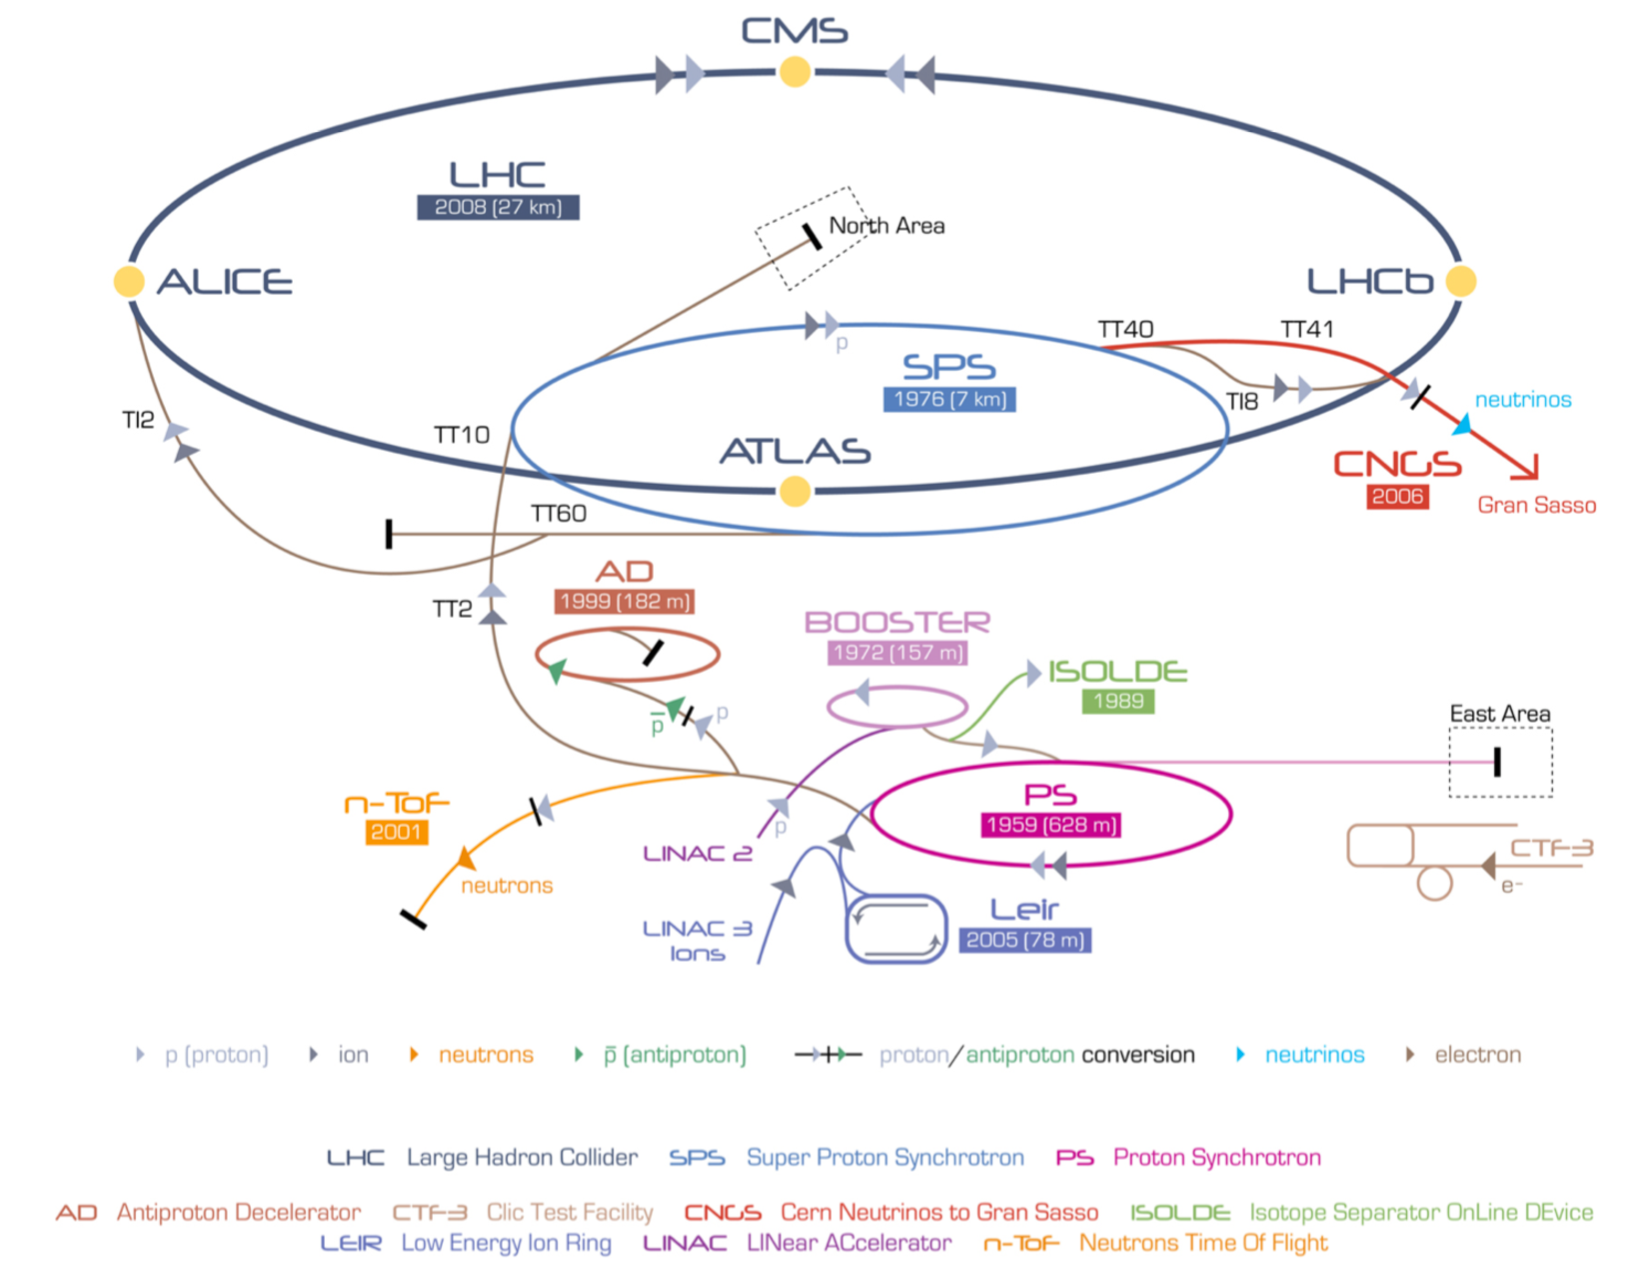
\includegraphics[width=0.75\textwidth, trim=2cm 0cm 1cm 1cm,clip]
                  {CERNaccelerators}
  \caption{The CERN experiments and accelerators.  This figure is taken
    from~\cite{cernaccel}.}
  \label{fig::CERNaccelerators}
\end{figure}

The COMPASS spectrometer is a two-stage spectrometer.  The two stages are in
series where each stage contains various tracking detectors and a muon wall
filter at the end of each stage.  Any particles that penetrate through the
active area of either of the muon wall filters are with a high probability,
muons.  Both stages also contain an electromagnetic and hadron calorimeter.  The
stages are both centered around a strong spectrometer magnet used for
determining charged particle momentum.  The first stage downstream of the target
is the large angle spectrometer (LAS) and it is centered around the SM1 magnet,
which has an integrated field of 1~Tm.  This stage detects tracks with larger
polar scattering angles approximately between 26~mrad and 160~mrad.  The second
stage is the small angle spectrometer (SAS) and it detects particle tracks
having a scattering angle between roughly 8~mrad and 45~mrad.  This stage is
centered around the SM2 magnet which has an integrated field of 4.4~Tm. \par

The left and right side of the spectrometer are referred to by the mountains
that surround the spectrometer.  When looking down the beam line, the left side
is referred to as the Jura side, which roughly corresponds to the west side.
The right side is referred to as the Saleve side, which roughly corresponds to
the east side.  A graphic of the 2015 setup is shown in
Fig~\ref{fig::compassSpec}.\par

This chapter gives an overview of the general COMPASS data taking setup and
highlights the specific features in 2015.  All the data in this thesis was
obtained with the 2015 setup.  For a more thorough review of the spectrometer
see reference~\cite{compassSpec}.  This chapter is roughly organized by how the
data taking occurs and concludes with an extra section summarizing the unique
features of the 2015 Drell-Yan data taking conditions. \par

\begin{figure}[h!t]
  \centering
  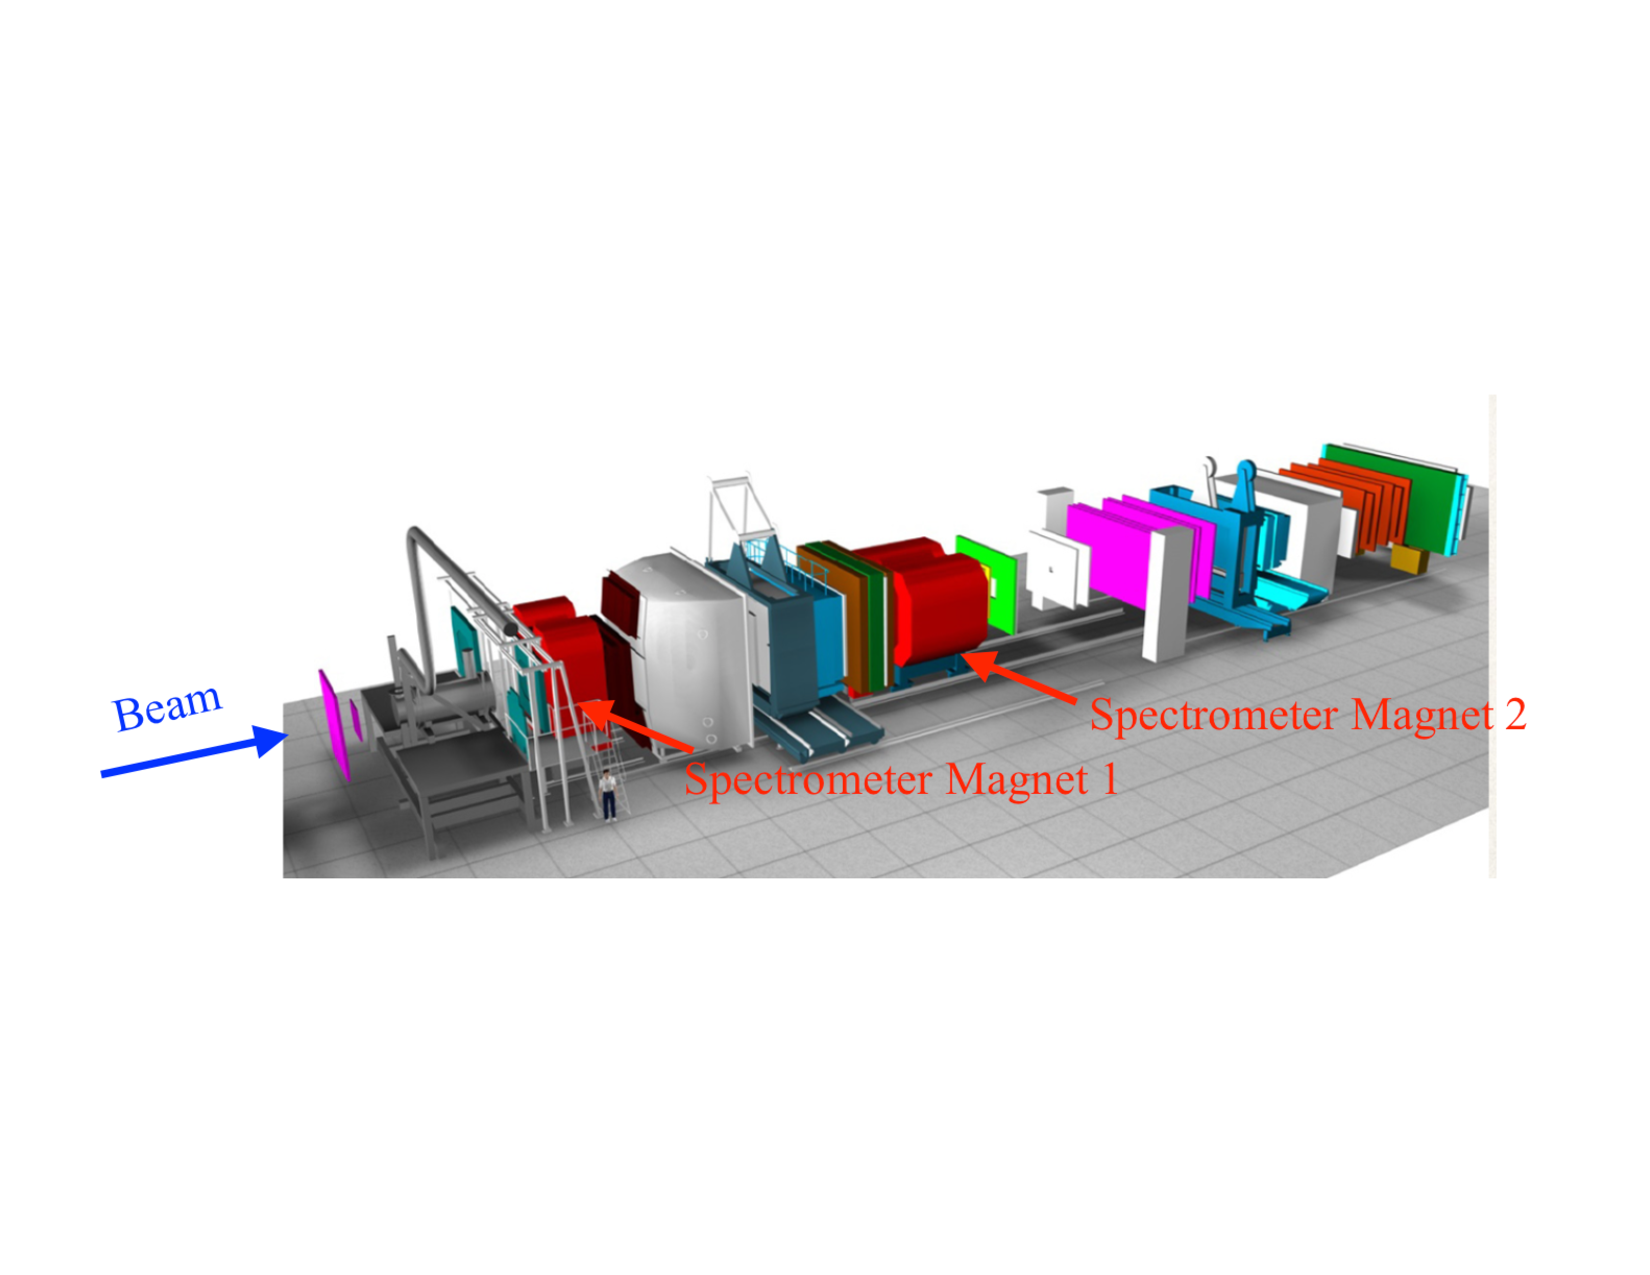
\includegraphics[width=\textwidth, trim=0.5cm 7cm 0.7cm 7cm,clip]{compassSpec}
  \caption{A schematic of the 2015 COMPASS setup.  This figure was taken
    from~\cite{compasswebpage}.}
  \label{fig::compassSpec}
\end{figure}

\section{The Beam}
The COMPASS spectrometer receives beam from the Super Proton Synchrotron along
the M2 beam line.  A schematic of the components in the M2 beam line is shown in
Fig.~\ref{fig::M2line}.  The SPS is the second largest accelerator at CERN with
a circumference of almost 7 km, which accelerates protons up to an energy of
450~GeV.  The SPS extracts beam to the famous Large Hadron Collier and as well
sends beam to various experiments in the North Area at CERN.  While the COMPASS
spectrometer is above ground, the SPS is below ground and the M2 beam line must
bend the beam from below ground to ground level. \par

There are several different beam types and energies available to COMPASS.  The
beam types used for the physics programs are a tertiary muon beam up to
190~{\gvc} and secondary hadron beam with an energy up to 280~{\gvc}.  Both of
the previous beam types can have a positive or negative charge.  As well as the
other two beam types it is also possible to have a low intensity tertiary
electron beam, mainly used for calibrations. \par

\begin{figure}[h!t]
  \centering
  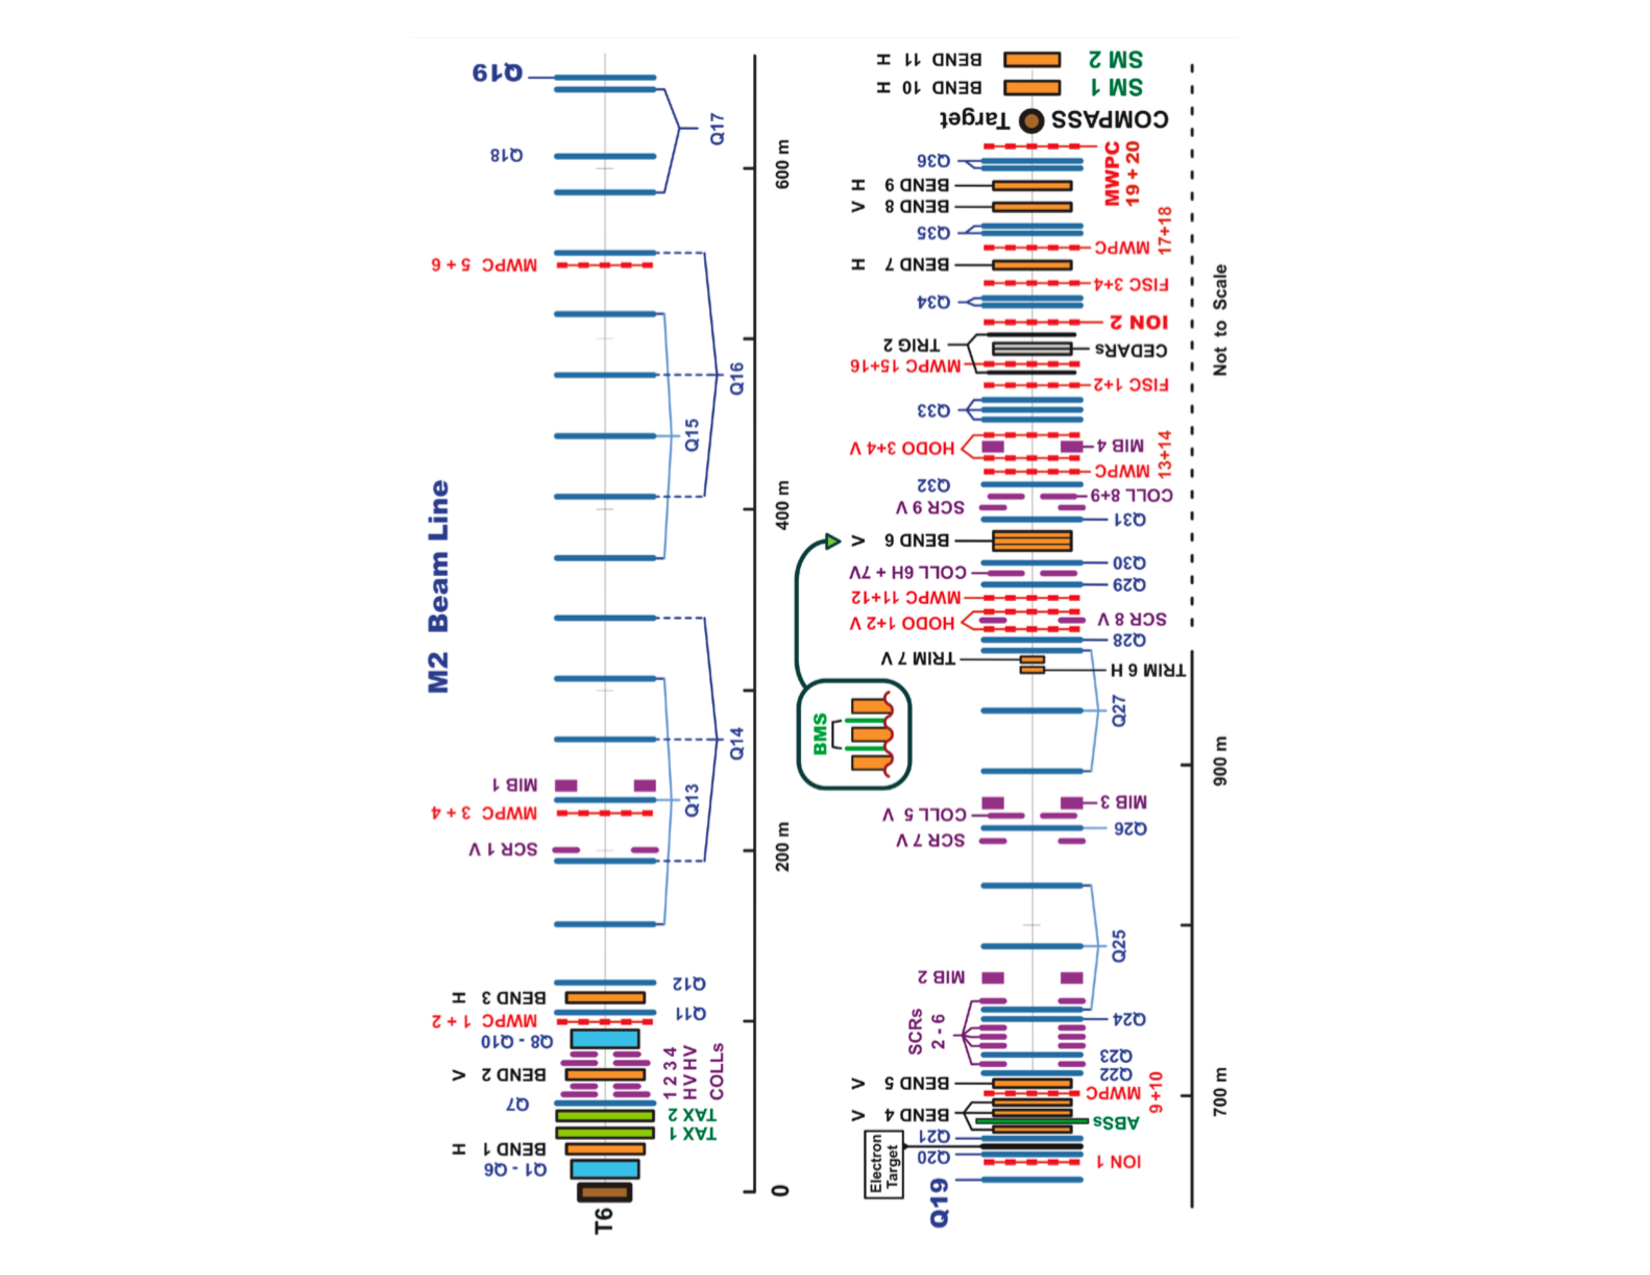
\includegraphics[width=\textwidth,trim=2cm 0cm 6cm 0cm,clip,angle=270]{M2line}
  \caption{The M2 beam line at CERN.  This image is taken
    from~\cite{ABBON201569}.}
  \label{fig::M2line}
\end{figure}

The beginning of the M2 beam line is the T6 target.  The SPS can accelerate
primary protons up to 400~{\gvc} to impinge on this T6 target, which produces a
secondary beam.  The nominal proton intensity on the T6 target is
100$\times 10^{11}$ spill$^{-1}$.  The T6 target is made of beryllium and has an
adjustable length.  The longer the T6 target the higher the secondary intensity,
where 500mm is the longest and typical target length used for physics data
taking.  The reaction of the proton beam with the T6 mainly produces secondary
protons, pions and kaons.  Following this reaction a series of dipole and
quadruple magnets select the momentum and charge of interest. \par

The SPS spill structure varies throughout the data taking year depending mainly
on the needs of the Large Hadron Colider (LHC).  In 2015, the average intensity
provided was 0.6$\times 10^8$ s$^{-1}$ and the typical spill structure was two
4.8~second spills every 36~seconds.

\subsection{Muon Beam}
The muon beam is a tertiary beam which results from a weak decay of the
secondary beam.  After the initial proton reaction on T6 the resulting secondary
particles are momentum and charge selected and sent through a 600m tunnel with
focusing and de-focusing (FODO) quadruple magnets.  In this tunnel the secondary
pions and kaons can decay as
\begin{equation}
  \pi^{-(+)} \rightarrow \mu^{-(+)} + \overline{\nu}_{\mu^-}(\nu_{\mu^+})
  \label{eqn::pionDecay}
\end{equation}
\noindent
and
\begin{equation}
  \mathrm{K}^{-(+)} \rightarrow \mu^{-(+)} +
  \overline{\nu}_{\mu^-}(\nu_{\mu^+}),
  \label{eqn::kaonDecay}
\end{equation}
\noindent
where K$^{-(+)}$ is a kaon of negative or positive charge.  At the end of the
tunnel, a series of nine 1.1~m long beryllium absorbers, referred to as the ABS
in Fig.~\ref{fig::M2line}, remove the remaining hadron component that did not
decay.  A 172~{\gvc} secondary pion beam is chosen to achieve a 160~{\gvc}
tertiary muon beam.  Due to the fact that the neutrino in the reactions
\ref{eqn::pionDecay} and \ref{eqn::kaonDecay} is always left handed, the muon
will naturally be longitudinally polarized.  For the muon momentum chosen, the
muon beam achieves a polarization of 80\%.

\subsection{Hadron Beam}
To deliver a hadron beam to COMPASS the ABS absorbers are not used.  The decayed
muons used for the tertiary muon beam have a lower momentum than the hadron beam
and are therefore removable by magnetically rejecting these lower momentum
muons.  In the case of a negative hadron beam as in 2015, the composition of the
beam is approximately 97~\% $\pi^-$, 2.5\% kaons and 0.5\%
$\overline{\mathrm{p}}$. The 2015 Drell-Yan data taking was performed with a
190~{\gvc} hadron beam. \par

\subsection{Additional Beam Line Components} \label{sec::addBeam}
After the decay tunnel the beam is bent upwards along another FODO tunnel.  The
lenght of this tunnel is 250m and reaches the surface level approximately 100m
before the COMPASS target.  A series of three dipole magnets, called bend 6,
then bend the beam to a horizontal position aimed at the COMPASS target.  Both
upstream and downstream of bend 6, there are three tracking detectors
(BM01-BM06) that make up the Beam Momentum Station (BMS).  The BMS is the
upstream most component of the COMPASS spectrometer.  It is able to determine
the beam momentum to better than 1\% of the beam momentum with an efficiency of
approximately 93\%.  Bend 6 and the BMS are shown schematically in
Fig.~\ref{fig::BeamLine1}. \par

\begin{figure}[h!t]
  \centering
  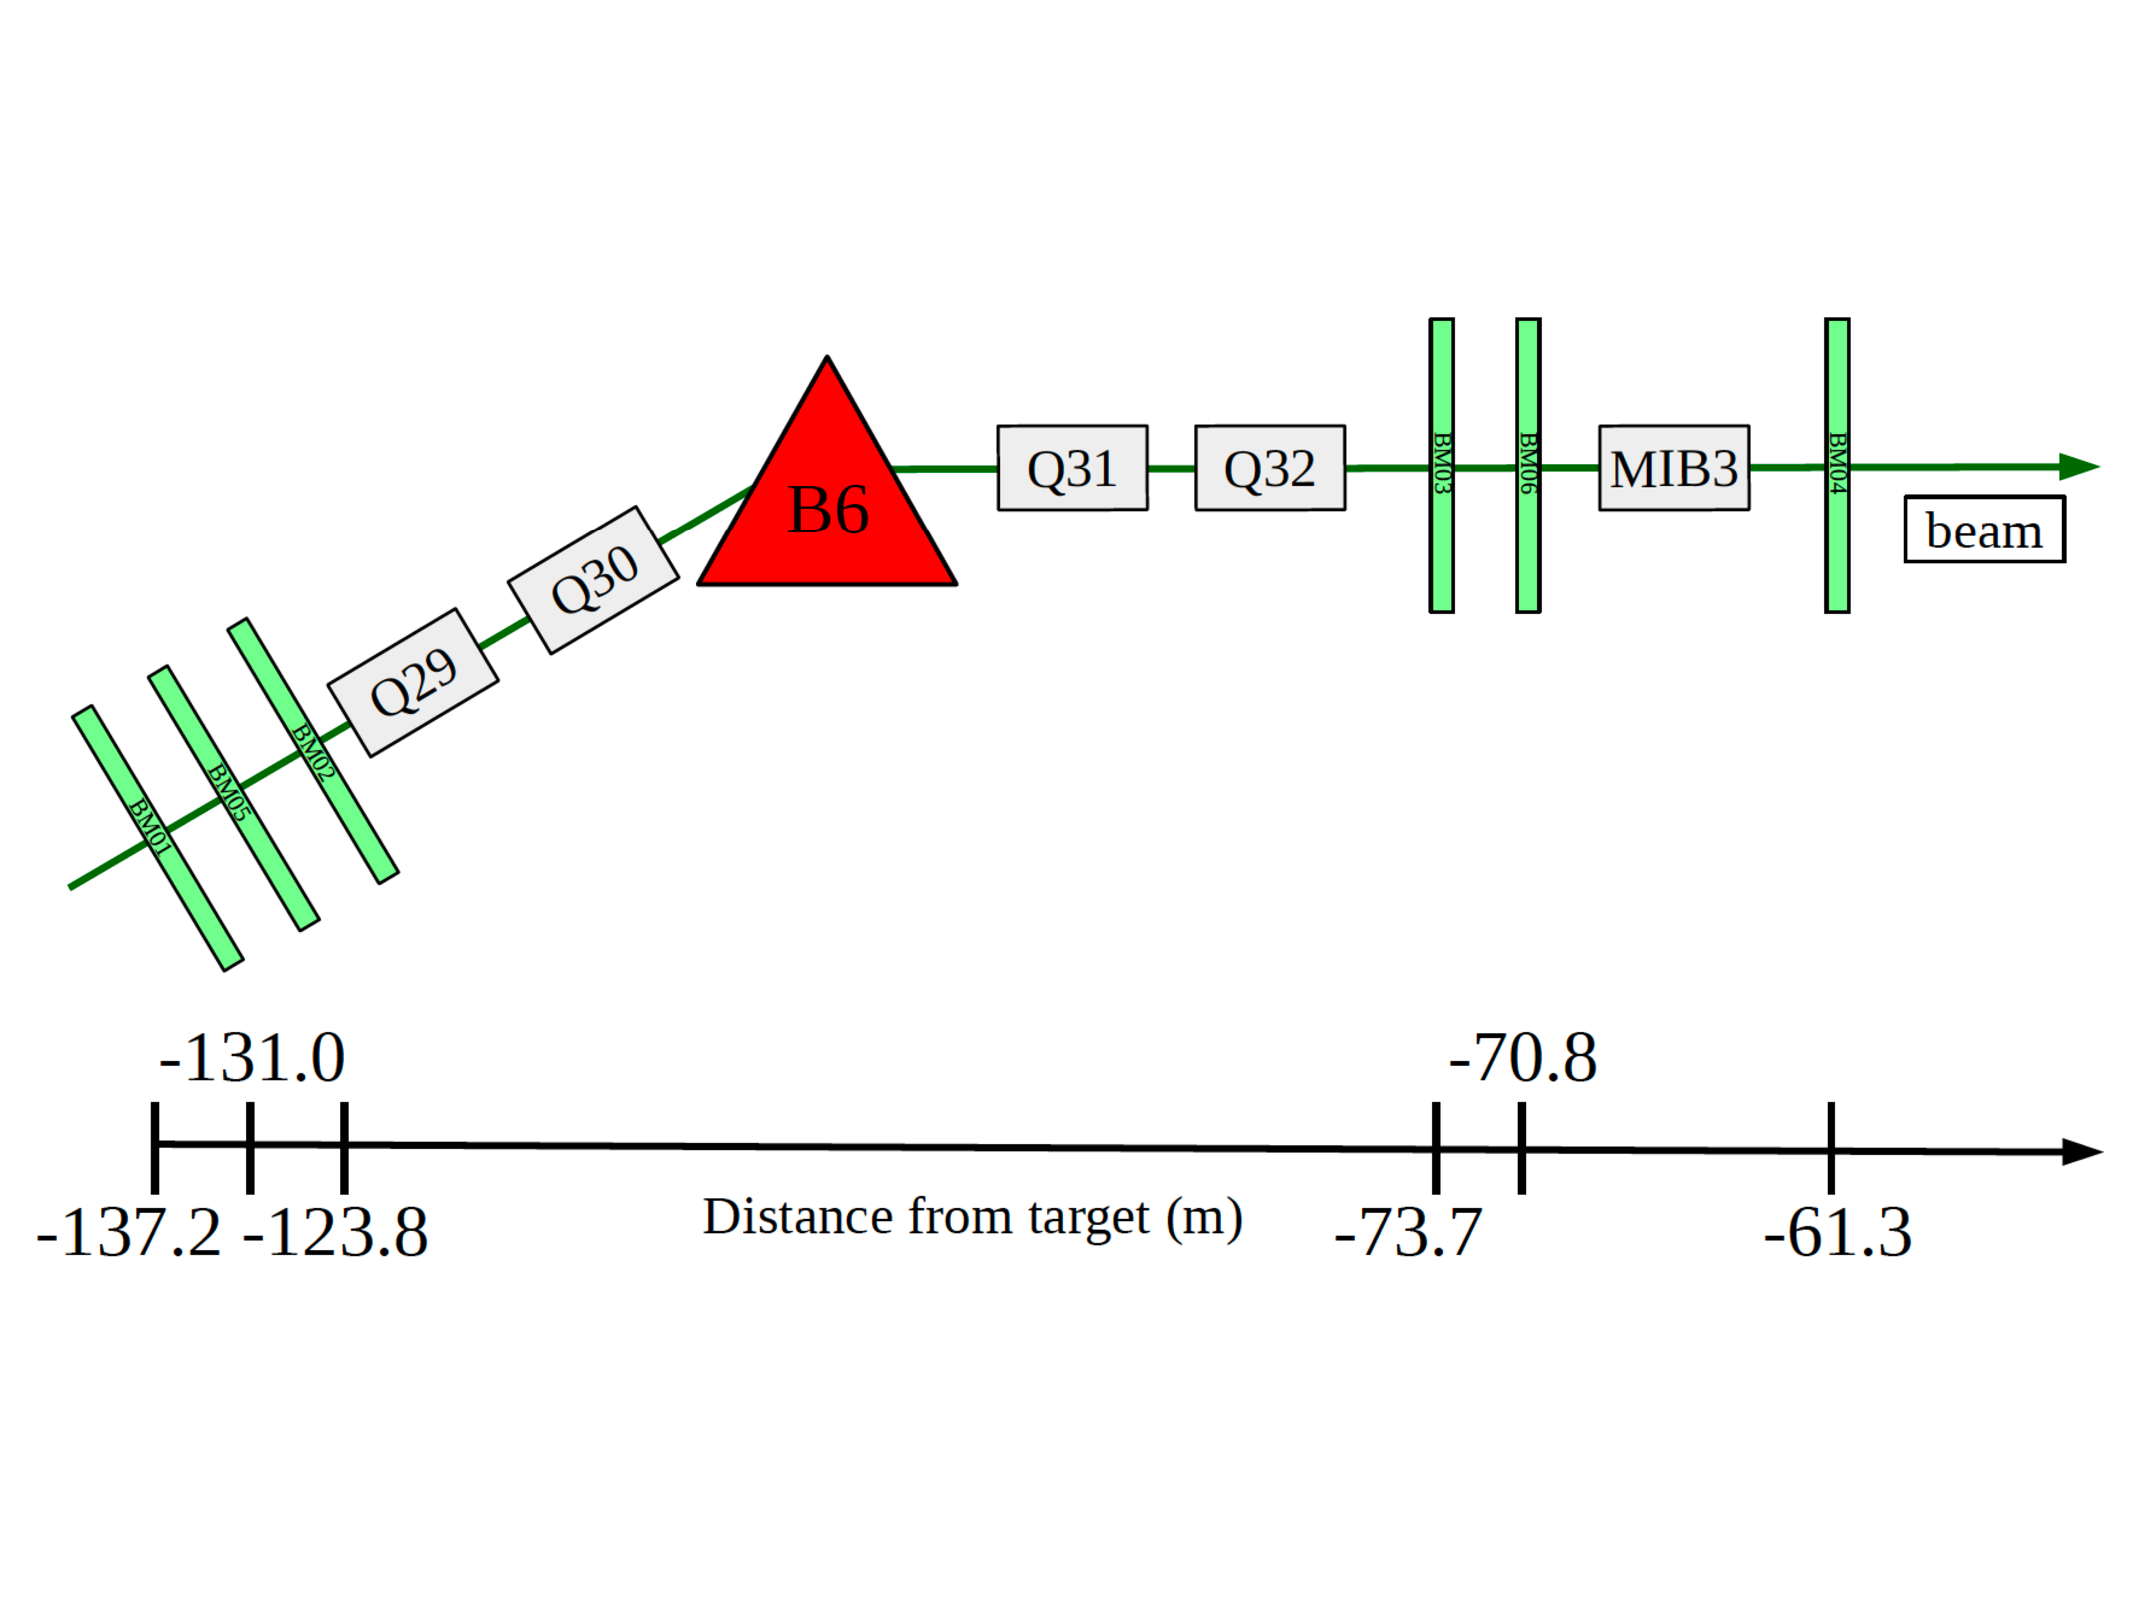
\includegraphics[width=0.8\textwidth]{BeamLine1}
  \caption{Bending the beam to a horizontal position.  The BMS detectors (green
    boxes) are upstream and downstream of the bend 6 magnet (red triangle
    labeled B6).  This image was taken from~\cite{compassSpec}.}
  \label{fig::BeamLine1}
\end{figure}

During the 2015 Drell-Yan setup the $\pi^-$ beam intensity was too high for the
BMS station to work properly.  For this reason, special low intensity,
approximately 10$^6$ s$^{-1}$, $\pi^-$ beams were used in 2014 to determine the
momentum distribution during Drell-Yan data taking.  The beam momentum
distribution is shown in Fig.~\ref{fig::BeamMomBMS}, where the average momentum
is 190.9~{\gvc} with a spread of $\pm$ 3.2~{\gvc}. \par

\begin{figure}[h!t]
  \centering
  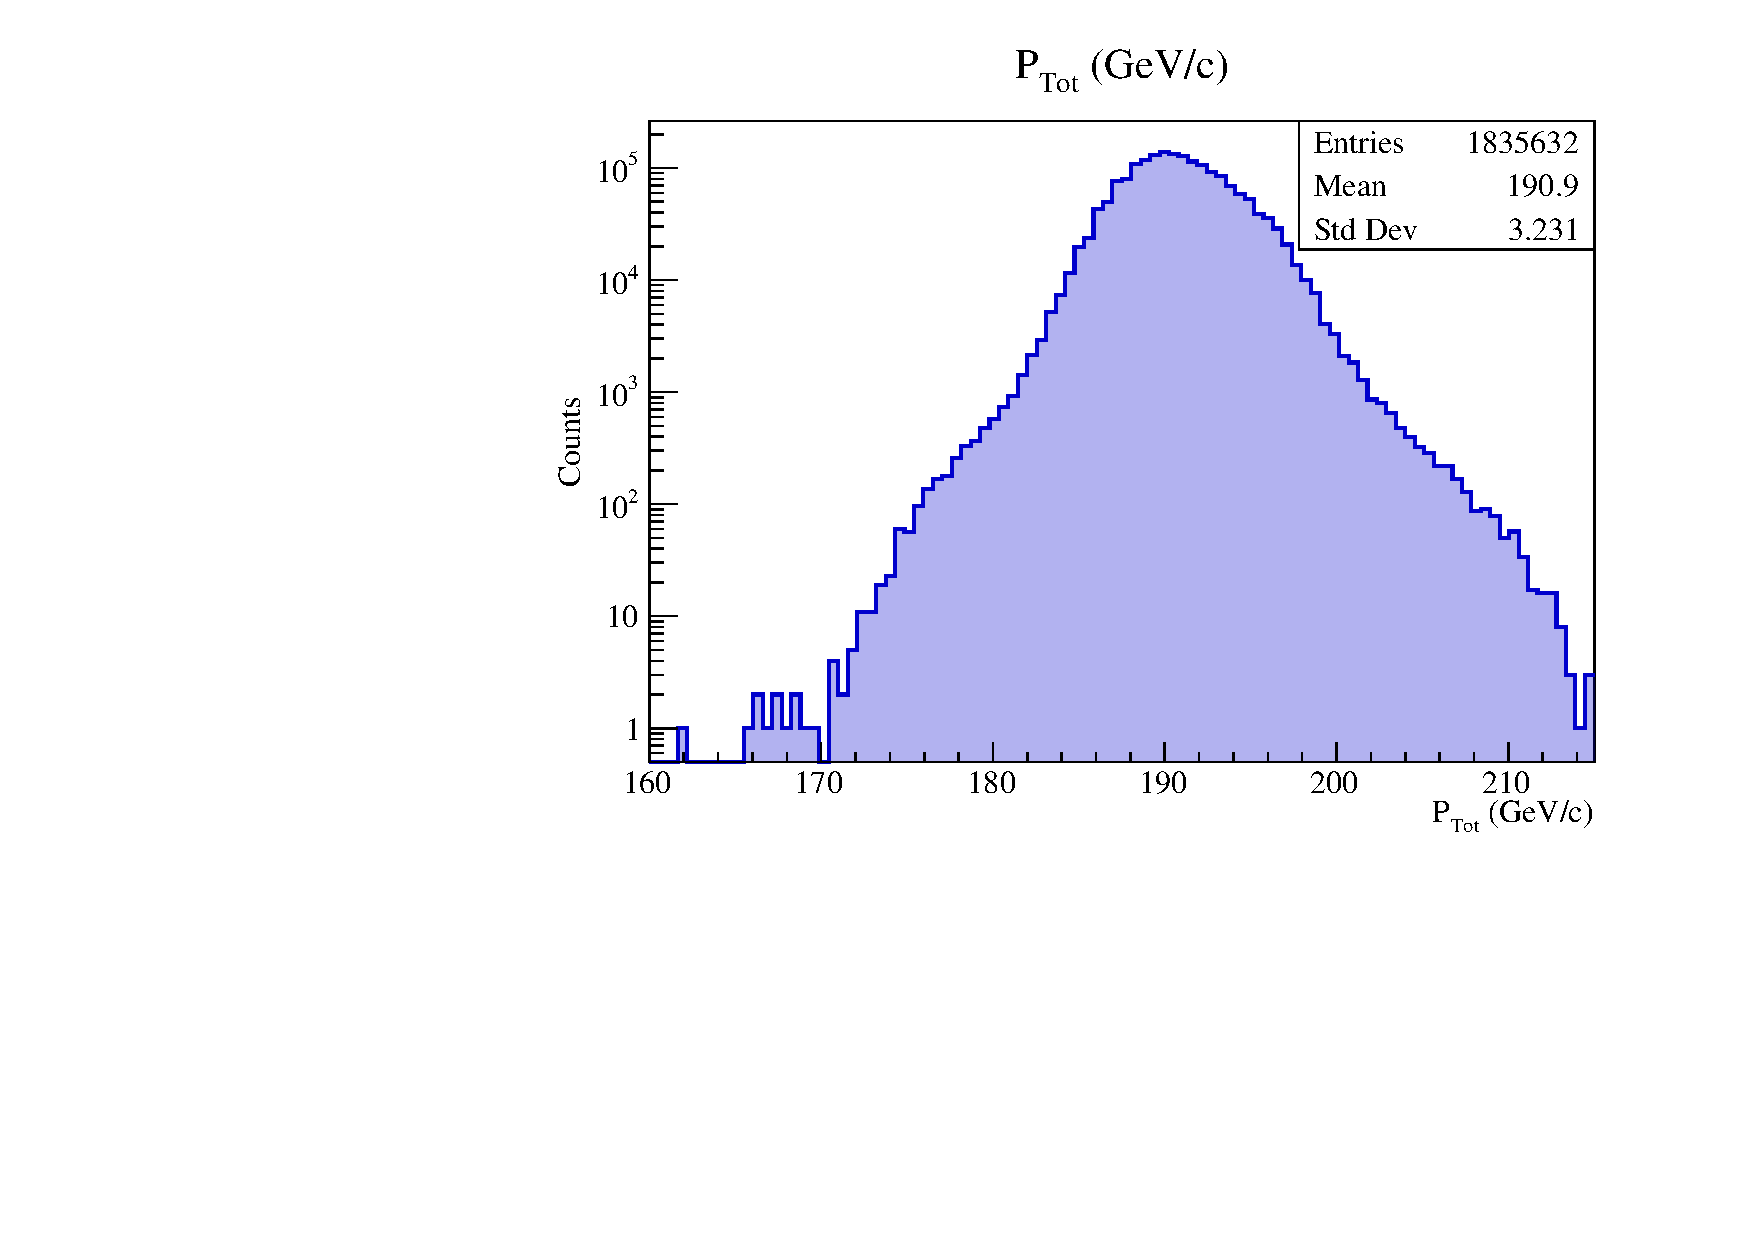
\includegraphics[width=0.5\textwidth]{BeamMomBMS}
  \caption{The momentum distribution of the $\pi^-$ beam, determined during
    dedicated low intensity beam conditions.  This figure was taken
    from~\cite{COMPbeamProp}.}
  \label{fig::BeamMomBMS}
\end{figure}

Approximately 30~m upstream of the target are to two Cherenkov counter (CEDAR)
detectors.  As the hadron beam has contamination from several components these
CEDARs can be used to distinguish between the different components.  The CEDARs
general principle of operation is that two particles with the same momentum but
different mass will emit Cherenkov radiation at different angles relative to
their momentum.  When a particle is traveling faster than the speed of light in
a given medium, it emits Cherenkov radiation in a cone centered along its
momentum axis.  The faster the particle is traveling, the narrower the angle of
the Cherenkov light cone.  A schematic of the CEDAR operating principle is shown
in Fig.~\ref{fig::cedars}.  In 2015 the CEDARs were measured to be largely
inefficient due to the high beam intensity and are not used for the analysis of
this thesis.

\begin{figure}[h!t]
  \centering
  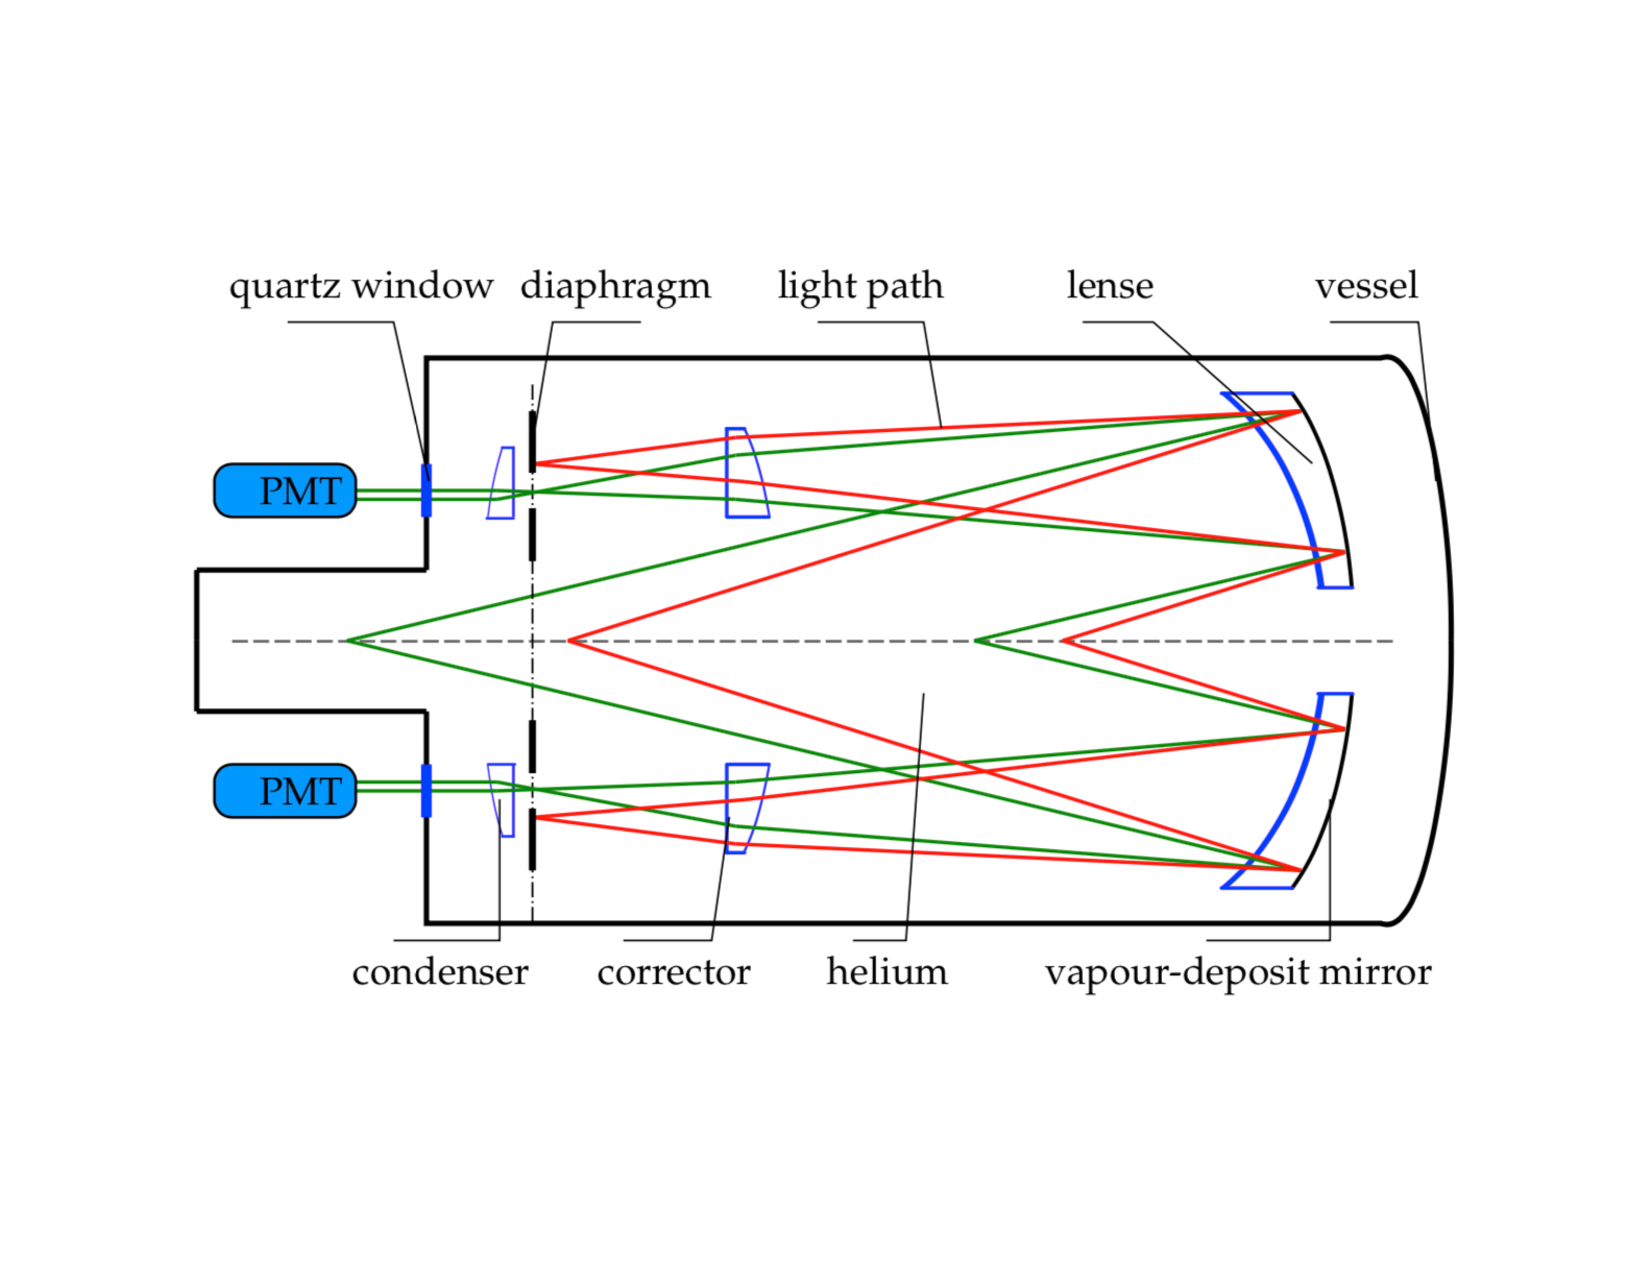
\includegraphics[width=0.5\textwidth,trim=2cm 4cm 2cm 4cm,clip]{cedars}
  \caption{Light lines emitted inside CEDARs at COMPASS.  The red(green) lines
    correspond to Cherenkov light emitted from a particle lower(higher)
    momentum.  This image is taken from~\cite{ABBON201569}.}
  \label{fig::cedars}
\end{figure}

For years with a transversely polarized target, such as 2015, a chicane system
of dipole magnets is setup in front of the target.  The chicane first bends the
beam away from the beam line and then back to the target such that the beam hits
the target at an angle.  A chicane magnet setup is used because a beam hitting
the target without any angle would then be deflected from the target magnet to
the left or right of the spectrometer.  For this reason the chicane gives the
beam an angle before hitting the target such that the non-interacting beam exits
the target traveling straight towards the spectrometer.


\section{The Polarized Target} \label{sec::polTarget}
The polarized target at COMPASS is the most complicated and essential component
of the spectrometer.  It is located upstream of the tracking detectors and
spectrometer magnets and downstream of the beam telescope detectors, described
in section~\ref{sec::tracking}.  The target consists of two or three cylindrical
cells.  The possible materials are either solid state ammonia (NH$_3$) or
deuterated lithium ($^6$LiD) or liquid
hydrogen~\cite{Matousek:2017rvj,Koivuniemi:2015uyw,GenkiPolTarget}.
Fig.~\ref{fig::PT} shows a schematic of the target.  \par

\begin{figure}[h!t]
  \centering
  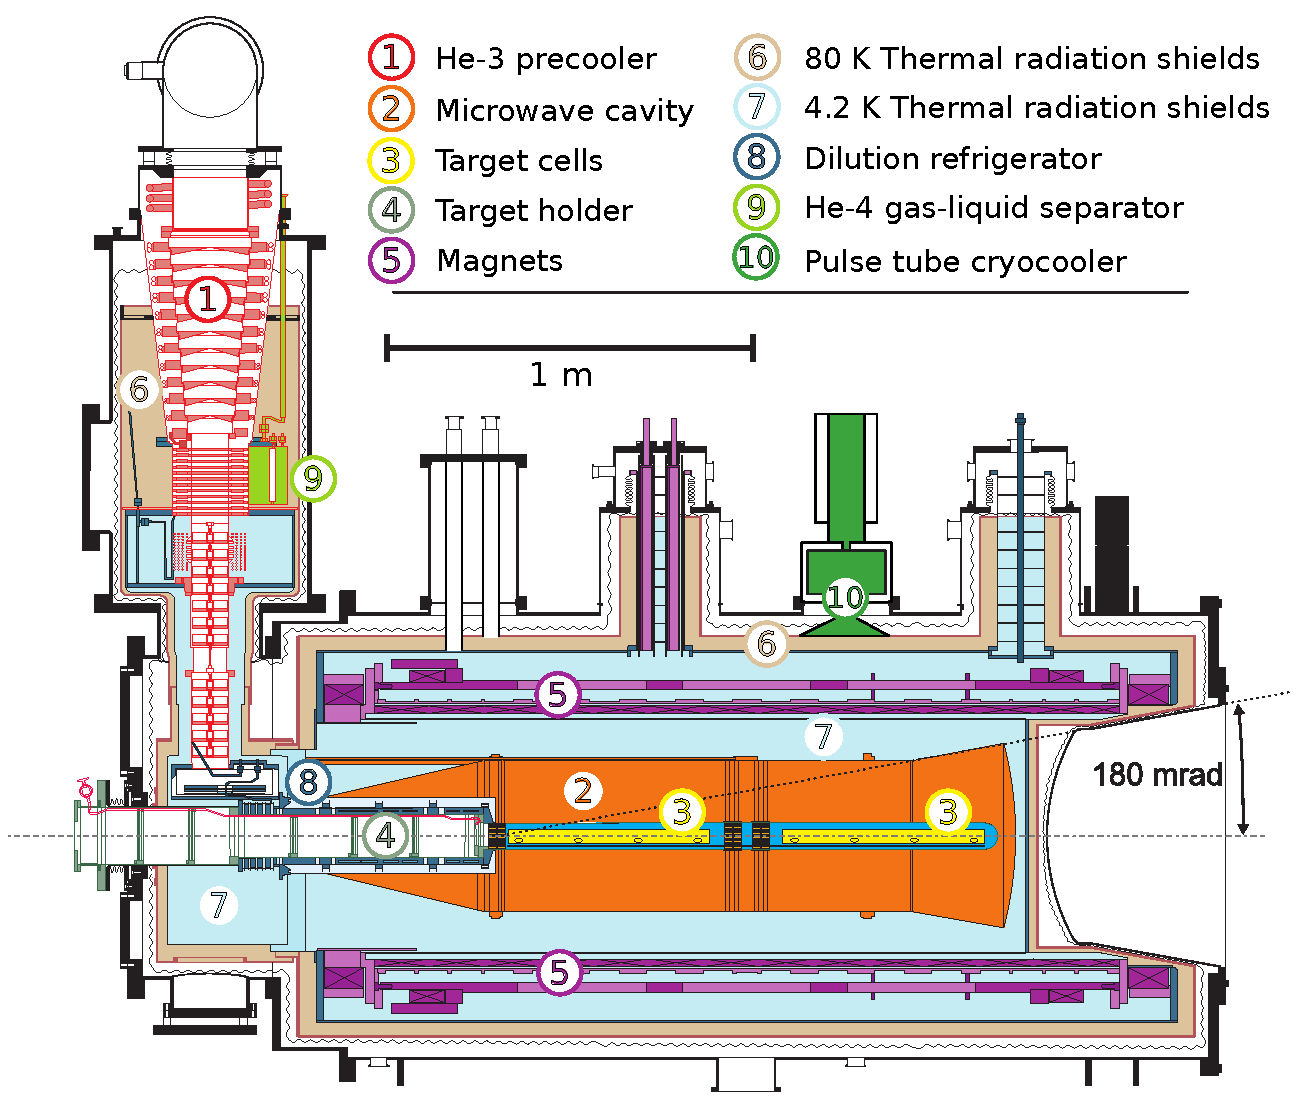
\includegraphics[width=0.8\textwidth]{PT}
  \caption{The polarized target at COMPASS.  This image taken
    from~\cite{Matousek:2017rvj}.}
  \label{fig::PT}
\end{figure}

Surrounding the cylindrical cells is a longitudinal super-conducting magnet
capable of reaching a magnetic field of 2.5~T.  This longitudinal magnet
polarizes the protons or deuterons in the target material parallel or
anti-parallel to the spectrometer axis.  The target polarization is
maintained by keeping the target in a liquid helium bath of approximately 60~mK.
This is called frozen spin mode where the temperature is maintained by a
dilution refrigerator. \par

The target is polarized through the dynamic nuclear polarization (DNP)
method~\cite{DNPmethod}.  This process works by first polarizing electrons in
the target with the longitudinal magnet.  With a high probability, the target
electrons are all polarized in the same longitudinal direction for each target
cells.  Due to their much lower mass, electrons have a larger magnetic moment
and therefore can be polarized at a much faster rate than protons or neutrons.
At the same time the electrons are being longitudinally polarized, microwave
electromagnetic radiation is sent through each target cell.  For atoms that have
a nuclear spin it is then possible to absorb a microwave and go to an excited
state with the electron spin anti-parallel to the magnet field direction and the
nuclear spin either parallel or anti-parallel to the magnet field direction
depending on the microwave frequency.  To ensure only one frequency enters each
target cell, there is a microwave stopper between each target cell.  The
electron with the anti-aligned spin will then quickly have its spin realigned
while the nucleon will take much longer to lose its polarization due to its
smaller magnetic moment.  This process can continue in this way resulting in a
net nuclear polarization.  Using the DNP method the target proton or deuteron
can achieve a polarization of approximately 90\% in three days. \par

The target also includes a 0.63~T transverse dipole magnet to change from
longitudinal to transverse polarization.  The target must first be
longitudinally polarized before the transverse target magnet can change the
polarization direction.  Once the target is transversely polarized, the target
polarization can no longer be increased as microwaves can no longer shine on the
target in the polarization direction.  Therefore the polarization will decrease
exponentially.  In 2015 the target was polarized for about half a day between
data taking sub-periods and achieved an average polarization of 0.73\%,
including the effects of exponential polarization loss with time.  The
relaxation time of the target polarization was about 1000 hours in 2015. \par

The target polarization was measured with 10 NMR coils while the target cells
were longitudinal polarized.  In the 2015, each target cell had the most
upstream and downstream coils in the center of the target cell and the other
three coils on the outside perimeter as is shown in Fig.~\ref{fig::targCells}.
Due to the fact that the polarization can only be measured with the longitudinal
magnet on, the polarization is only measure at the start and finish of a
transversely polarized data taking.  The intermediate polarization is then
determined by exponential interpolating between these two times.

\begin{figure}[h!t]
  \centering
  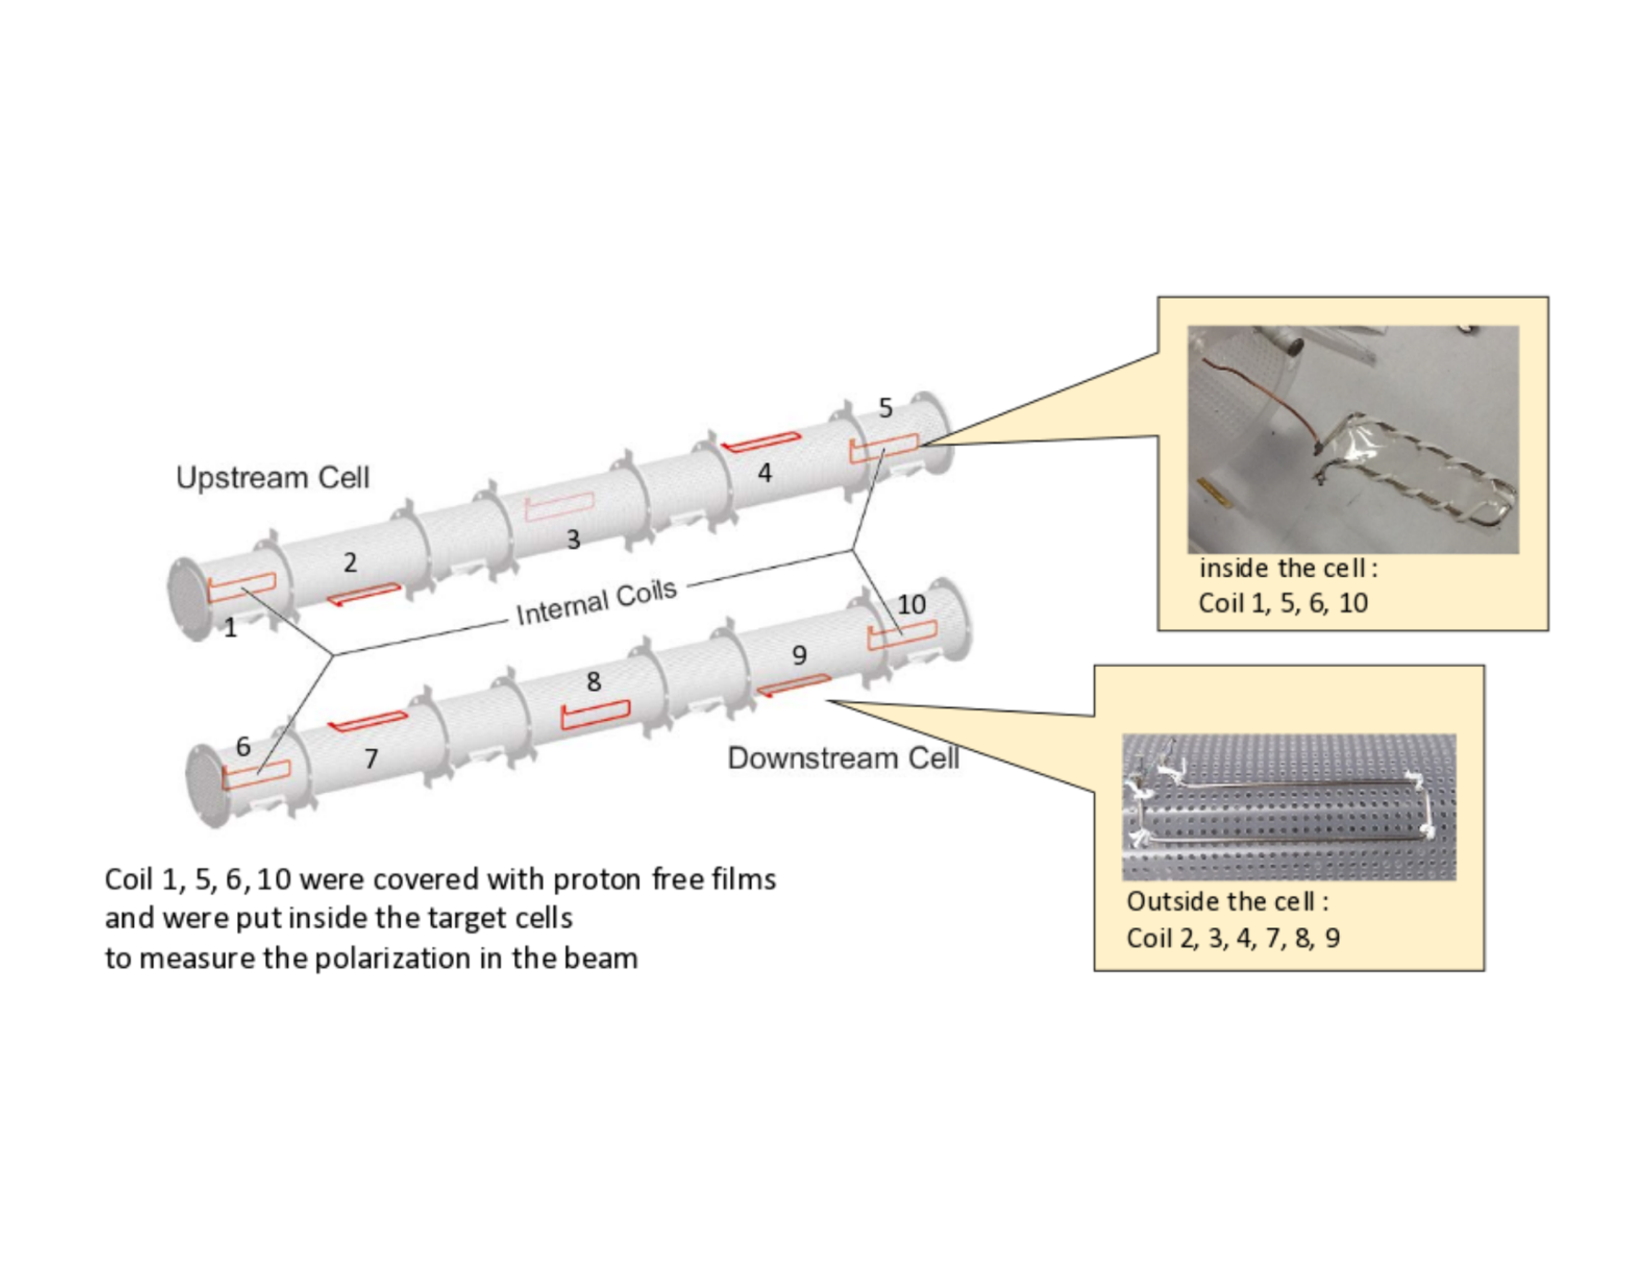
\includegraphics[width=0.8\textwidth]{targCells}
  \caption{The empty polarized target cells side by side along with their NMR
    coil positions.  This image taken from~\cite{polTargCells}.}
  \label{fig::targCells}
\end{figure}

In 2015 the setup was two transversely polarized target cells of 55~cm length
and 2~cm in radius.  The cells were separated by 20~cm and polarized in opposite
directions.  The polarization of the target cells was flipped ever two weeks of
data taking to reduce systematic effects from luminosity and geometrical
spectrometer acceptance.  Due to the fact that the beam needs to be precisely
steered onto the target and that the chicane magnets upstream of the target are
setup for only one transverse target magnet direction, the transverse target
magnet only pointed downward in 2015.  To achieve a polarization flip the target
polarization had to therefore be rotated back to the longitudinal direction and
the input microwaves had to be changed to achieve the desired polarization
direction. \par

The target material in 2015 was solid state NH$_3$.  The protons in the three
hydrogen atoms were the only nucleons with nuclear spin and therefore only some
fraction of the target was able to be polarized.  The fraction of polarized
nucleons to total nucleons is called the dilution factor.  Counting the ratio of
unpolarized nitrogen nucleons to polarized hydrogen, one would expect the
dilution to be 3/17.  However to get a more accurate determination of the
dilution factor the follow calculation was used

\begin{equation}
  f = \frac{n_H\sigma^{DY}_{\pi^-H}}
  {n_h\sigma^{DY}_{\pi^-H} + \sum_A n_A\sigma^{DY}_{\pi^-A}},
  \label{equ::dilution}
\end{equation}
where $f$ is the dilution factor, $n_H$ is the number of hydrogen atoms in
NH$_3$, $n_A$ is the number of other nucleons in NH$_3$, and
$\sigma^{DY}_{\pi^-H}$ and $\sigma^{DY}_{\pi^-A}$ are the Drell-Yan
cross-sections for pion-hydrogen scattering and pion-nucleon scattering
respectively.  The cross-sections were determined using a parton-level
Monte-Carlo program MCFM~\cite{MCFM}.  The dilution factor was also further
scaled down by studies of reconstruction migration between target cells.  The
average dilution factor in 2015 was determined to 0.18 in the invariant mass
range of 4.3{\gvcs} to 8.5{\gvcs}.


\section{Tracking Detectors} \label{sec::tracking}
To determine when and where a reaction occurs in the polarized target, tracking
detectors are able to position the products of the reaction.  The goal of the
tracking detectors is to determine a point in space where a particle traversed.
The COMPASS tracking detectors attempt to do this for a wide range of angles,
momenta and at different rates.  For these reasons there are several planar
tracking technologies used at COMPASS that can be divided into three
categories: very small angle trackers, small angle trackers and large area
trackers.  As the name suggests, very small angle trackers measure tracks with
small angle deflections from the beam axis which are essentially beam particles.
The small area trackers measure particle tracks with low but non-zero scattering
polar angle and have small central dead zones.  The large area trackers are
several meters in height and width and measure the largest deflection angles up
to 180~mrad. \par

All of these trackers are split into stations.  Each station corresponds to
several detectors planes at roughly the same z-position along the beam line.
Each station measures a track position in one or more orientation while most
measure tracks in three or more orientations.  The coordinate orientations
measured are the X and Y coordinates, which are the horizontal and vertical
directions respectively, and as well the U and V coordinates which are rotated
at different angles with respect the X and Y coordinates. \par

\subsection{Very Small Angle Trackers}
The very small angle trackers extend up to 3~cm away from the beam axis.  This
is the region with the highest number of particles and therefore these
detectors must be able to handle the highest rates up to 5x10$^7$~Hz.  The two
detector types that make up the very small angle trackers are either
scintillating fiber detectors (SciFi) or silicon microstrip detectors.  These
two detector types are complementary to each other as the former have very good
timing resolution, while the latter have very good spacial resolution. \par

There are three silicon stations possible at COMPASS.  These stations have
active detecting areas of 5x7~cm$^2$.  The spacial resolution of these detectors
is nominally 10~$\mu$m and the timing resolution is nominally 2.5~ns.  For the
2015 setup, the beam intensity was too high for the silicon detectors to operate
and therefore these detectors were not used. \par

There are 10 SciFi stations available at COMPASS.  The active areas vary from
3.9x3.9~cm$^2$ to 12.3x12.3~cm$^2$ planar areas.  As well the detection fiber
diameters vary between detectors with the different diameters used at COMPASS
being 0.5~nm, 0.75~nm and 1~nm.  Several fibers are bundled together to
determine a strip hit position and the resulting nominal spacial resolutions are
130~$\mu$m, 170~$\mu$m and 210~$\mu$m respectively.  The nominal timing
resolution of these detectors is about 400~ps.  In 2015 three SciFi stations
made up the beam telescope and were placed upstream of the target to measure the
beam trajectory and timing information.  A fourth SciFi station was place in the
LAS section of the spectrometer. \par

\subsection{Small Angle Trackers} \label{sec::SAT}
The small angle trackers detect particles with non-zero defection angles. These
detectors have medium size active areas compared to the very small angle
trackers and the large angle trackers.  They cover 5~cm to 40~cm from the beam
axis where the rate drops to approximate 10$^5$~Hz, two orders of magnitude
lower than the rates the very small angle trackers receive.  At COMPASS there
are two types of small area tracking detectors: micromesh gaseous structure
(micromegas) and gas electron multipliers (GEMs). \par

There are three micromega stations at COMPASS.  All three stations are located
sequentially after each other between the target and the first spectrometer
magnet.  As well all three detectors measure four coordinate projections and
have an active area of 40x40~cm$^2$ with a 5~cm diameter dead zone.  The
micromegas operate by having a conversion region and a smaller amplification
region.  An ionized particle produced in the conversion region will drift
through an electric field of around 3.2~kV/cm to the amplification region where
the electric field is around 50~kV/cm.  The electric field is too small for
amplification in the conversion region but as the name suggest the electric
field is high enough to amplify the signal in the amplification region.  The
amplified signal is then read out on strips.  The conversion and amplification
regions are separated by a metallic micromesh material.  The electrons pass
through the micromesh without resistance and are not rimmed out.  The micromegas
have good spacial resolution because the thickness of the amplification region
is only 100~$\mu$m, small enough to prevent much transverse spreading of the
electron avalanche between strips.  The separation of the larger conversion
region from the smaller amplification region with the micromesh prevents
electric field lines from being distorted in the conversion region and therefore
prevents the primary electrons from drifting slower in the conversion region.
This allows micromegas to operate at a higher rate than would be possible
otherwise.  This principle of operation is illustrated in
Fig.~\ref{fig::MicroMega}.  The strips in the central part of the detector are
360~$\mu$m corresponding to a position resolution of about 100~$\mu$m and the
strips in the outer region are 460~$\mu$m corresponding to a resolution of about
120~$\mu$m.  The nominal timing resolution is 9~ns.  In 2015 the micromegas were
upgraded to include a pixelized section covering much of the dead zone
area. \par

\begin{figure}[h!t]
  \centering
  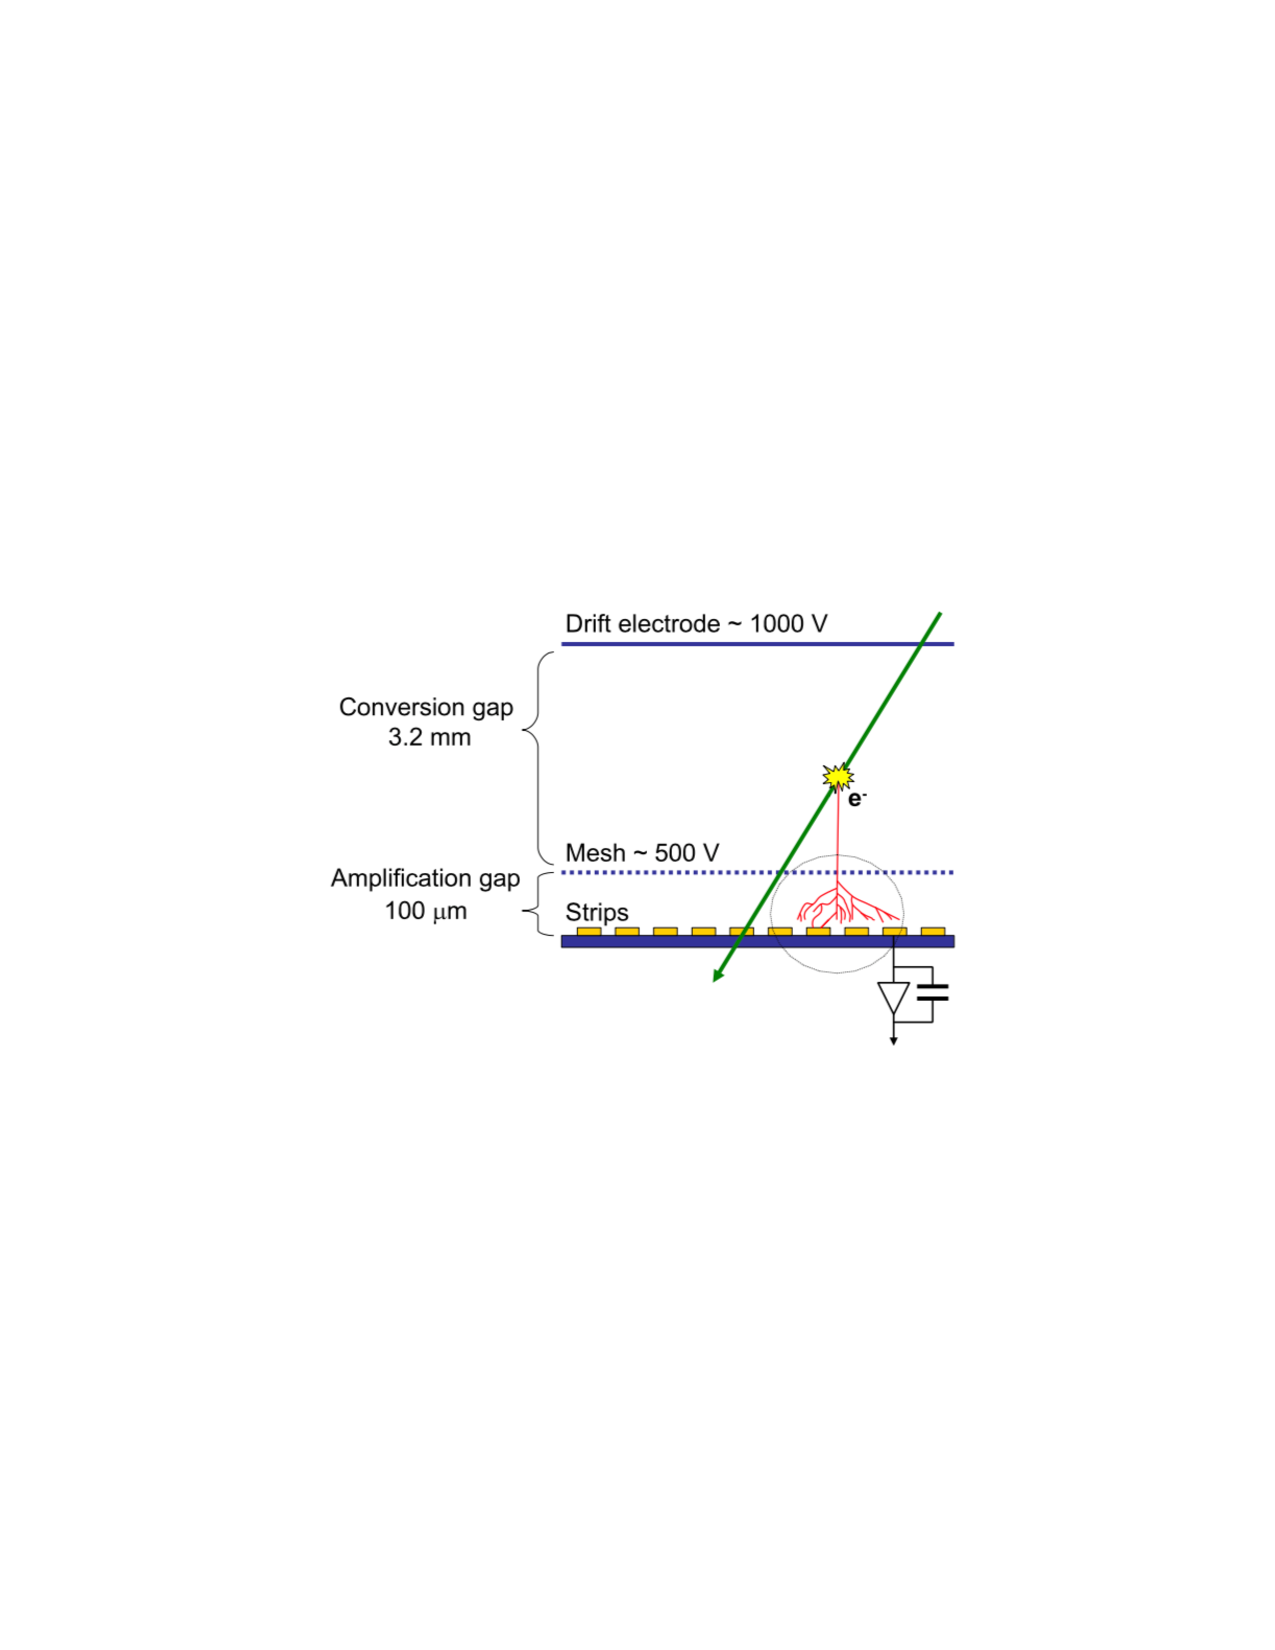
\includegraphics[width=0.7\textwidth, trim=4cm 10cm 4cm 10cm, clip]{MicroMega}
  \caption{Principle of operation for the micromesh gaseous structures
    (micromegas).  This image was taken from~\cite{compassSpec}.}
  \label{fig::MicroMega}
\end{figure}

There are eleven GEM detectors located throughout the COMPASS spectrometer.  The
first GEMs are located after the first spectrometer magnet and the last GEMs are
located near the end of the spectrometer.  These detectors are positioned close
to the beam axis.  Each of them is mounted on a large area tracker, covering the
dead zone region of the large area tracker.  All eleven detectors have an active
area of 31x31~cm$^2$ and a 5~cm diameter dead zone.  In times of lower beam
intensity, such as alignment runs, the dead zones can be turned on as an active
area.  \par

The GEM detectors are split into four regions where each region is separated by
a polymide foil (50~$\mu$m thick).  The polymide foil has approximately
10$^4$~cm$^{-1}$ drifting holes of 70~$\mu$m diameter, which are clad with
copper on both sides.  There is an electric potential of a few hundred volts
between each pair of foil layers.  The electron amplification occurs around the
holes of each of the three foil dividers.  This means GEM detectors speed up the
amplification process by splitting the amplification avalanche into three
locations.  The process is sped up because the drifting electrons are
accelerated multiple times, thereby speeding up their drifting velocity which
therefore reduces the overall drift time from the ionization location to the
strip readout.  This allows the GEMs to operate at a higher rate then would
otherwise be possible.  The principle of operation is illustrated in
Fig.~\ref{fig::GEM}.  The nominal timing and spacial resolution of the GEM
detectors is 10~ns and 110~$\mu$m respectively.  Two pixelized GEM detectors
were also in operation but were not as crucial for the 2015 Drell-Yan
measurement.

\begin{figure}[h!t]
  \centering
  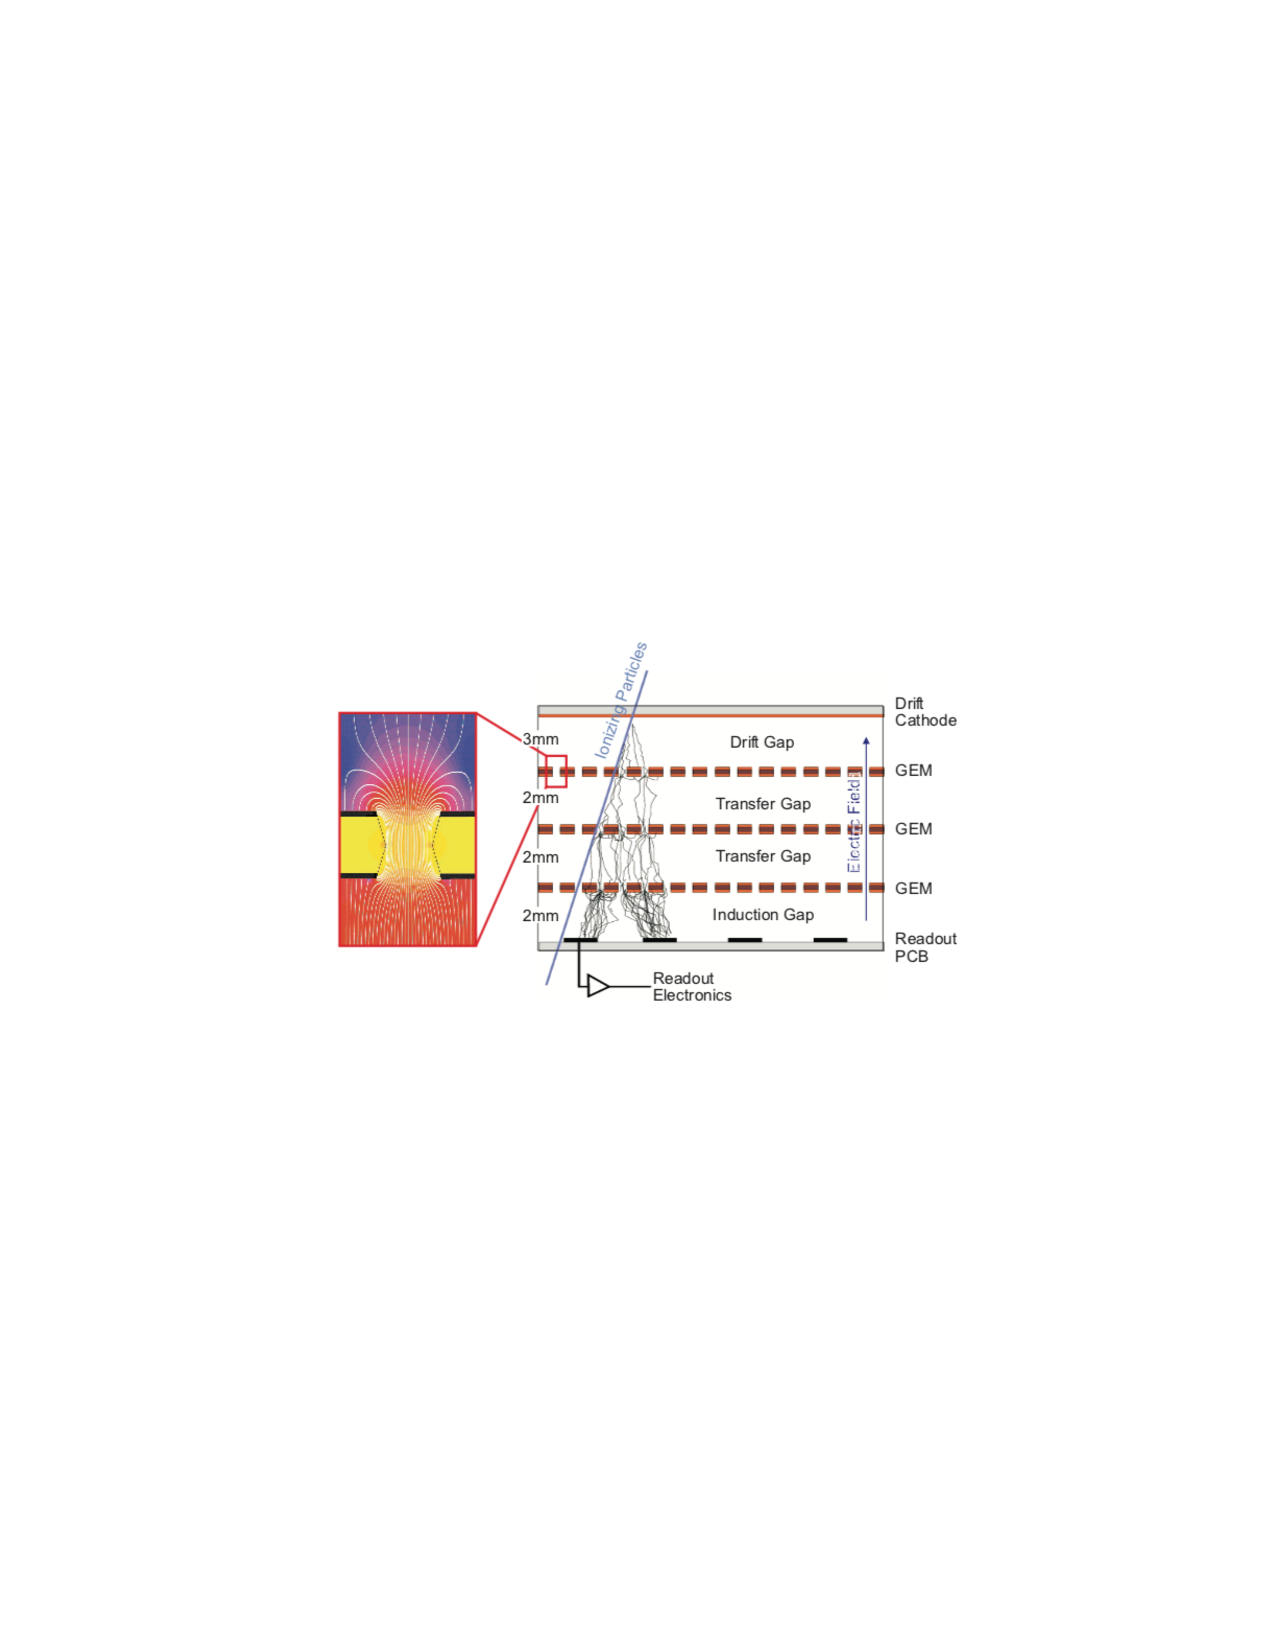
\includegraphics[width=0.7\textwidth,trim=4cm 10cm 4cm 10cm, clip]{GEM}
  \caption{The operation principle of the gas electron multiplier (GEM)
    detectors.  This image was taken from~\cite{compassSpec}.}
  \label{fig::GEM}
\end{figure}

\subsection{Large Area Trackers}
The large area trackers measure the largest polar scattering angles at COMPASS.
Their dead zones mostly coincide with a small area tracker, described in the
previous section~\ref{sec::SAT}, which therefore means these detectors do not
have to process the higher fluxes very close to the beam line.  The most
important feature of these detectors is that they have a large planar area. As a
consequence however, their position and timing resolutions are not as good as
the small and very small angle trackers.  The types of large area trackers used
at COMPASS are all gaseous detectors and include drift chambers (DCs), straw
tube detectors (straws) and multi-wire proportional chambers (MWPCs). \par

The first four drift chambers downstream of the target are named DC00, DC01,
DC04 and DC05.  The first two, DC00 and DC01, have smaller active areas of
180x127~cm$^2$ and a circular dead zone of 30~cm diameter.  These two drift
chambers are positioned upstream of the SM1 magnet.  The rates upstream of SM1
are higher.  This is due to the fact that low energy particles are produced in
the target, but are bent out of the acceptance of spectrometer by SM1.
Therefore the detectors downstream of SM1 do not track these low energy
particles and therefore DC00 and DC01 need to be able to process a higher
particle flux.  The next two drift chambers, DC04 and DC05, are downstream of
SM1 and both have larger active areas of 240x204~cm$^2$ and as well have dead
zones of 30~cm diameter.  The active areas of all four of these DCs was roughly
chosen to coincide with the acceptance of the SM1 yoke.  DC05 was first
installed for the 2015 Drell-Yan data taking and is further described in
chapter~\ref{ch::dc05}.  All four of these DCs measure four projection views
corresponding to eight detector layers.  A sketch of the principle of operation
is shown in Fig.~\ref{fig::DCoperation}.  The nominal spacial resolution for
these detectors is 250~$\mu$m. \par

\begin{figure}[h!t]
  \centering
  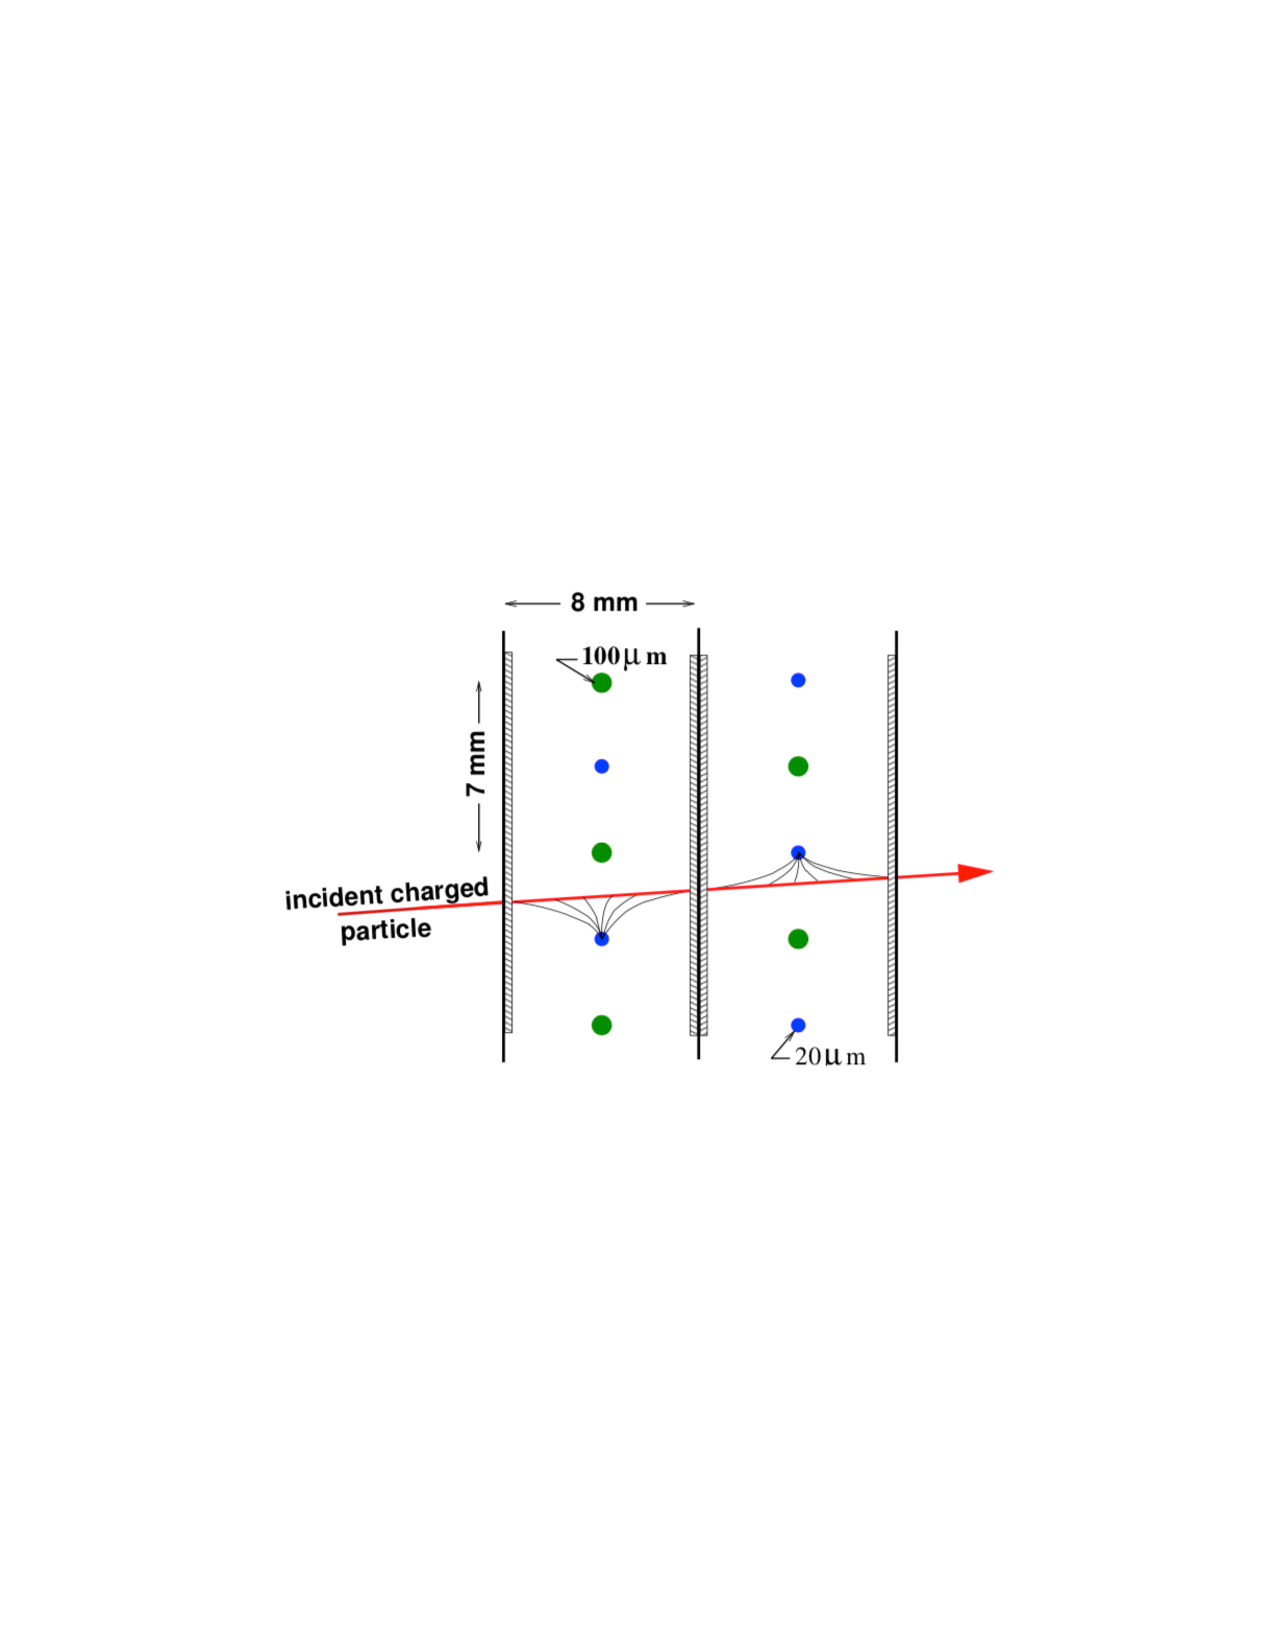
\includegraphics[width=0.6\textwidth,trim=4cm 8cm 4cm 10cm,
    clip=true]{DCoperation}
  \caption{Side view of a drift cell in a drift chamber with the ionized drift
    electron lines coming from the incident charged particle.  The larger
    circles (green) represent field wires and the smaller circles (blue)
    represent sense wires.  This image was taken from~\cite{compassSpec}.}
  \label{fig::DCoperation}
\end{figure}

Further downstream the spectrometer, downstream of the SM2 magnet, are the W45
drift chamber stations.  The W45 drift chambers are the largest drift chambers
at COMPASS.  There are six W45 detector stations, which each have an active area
of 520x260~cm$^2$ and a circular dead zone of 50~cm or 100~cm diameter.  Each
W45 station measures two projection views corresponding to four detector layers.
The drift cells in W45 are 40x10~mm$^2$ and the spacial resolution is nominally
1500~$\mu$m. \par

The two straw stations in operation during the 2015 data taking are named ST03
and ST05.  ST03 was in the large angle spectrometer downstream of DC05 and
consists of two stations measuring six projection views.  ST05 was in the small
angle spectrometer and measured three projection views.  The active areas of
each of the horizontal wire stations is 350x243~cm$^2$ and the active area of
each of the rotated wires is 323x272~cm$^2$.  The principle of operation for the
straw detectors is very similar to that of a drift chamber.  However, instead of
having the detector made up of connected drift cells the straw detectors are
made of separated circular tubes.  Each tube consist of a gold plated tungsten
anode wire in the center and the walls of the tube make up a cathode.  Due to
the fact that the cathode completely surrounds the anode wire there is no
electrical interference between neighboring anode wires as there is for drift
chambers.  For this reason the electric field in each tube is easier to control
and the ionized electron drift speed is more linear than other detectors.  Each
straw detector plane is divided into sections where the straw tubes in the outer
most section from the beam line have a diameter of 9.6~mm and the tubes close to
the beam line have a diameter of 6.1~mm.  In addition, in the central part of
the detector there is a physical hole, dead zone of 20x20~cm$^2$.  The nominal
position resolution for these detectors is 400~$\mu$m.  A frontal schematic is
shown in Fig.~\ref{fig::frontalStraw}.  For the reason that most of the detected
muons are reconstructed in the large angle spectrometer and the fact that many
of the high voltage modules were not operation for ST05 in 2015, ST05 was not
used for track reconstruction for 2015 Drell-Yan data. \par

\begin{figure}[h!t]
  \centering
  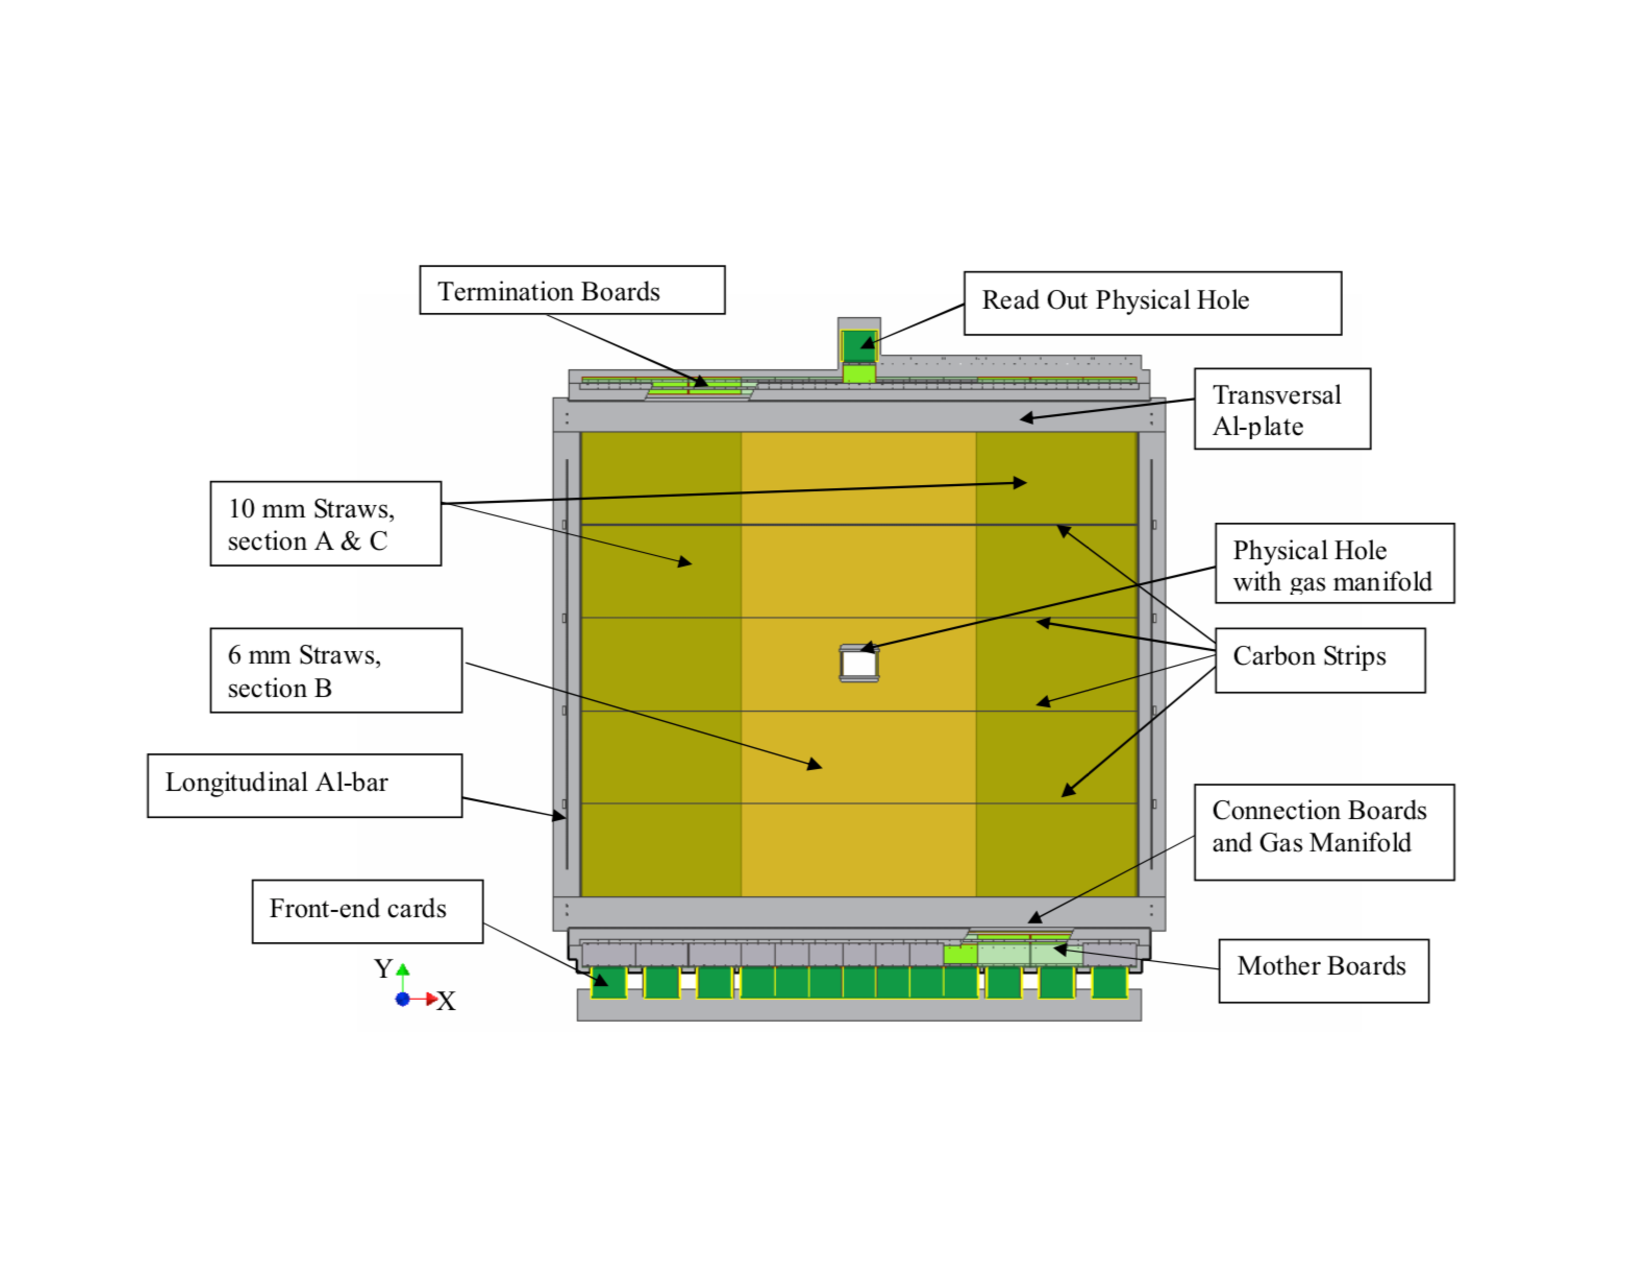
\includegraphics[width=0.8\textwidth,trim=2cm 4cm 3cm 4cm,clip]{frontalStraw}
  \caption{Front on view of a the active area of a straw detector at COMPASS.
    This image was taken from~\cite{compassSpec}.}
  \label{fig::frontalStraw}
\end{figure}

The next type of large angle track is the richwall.  This large area tracker
operates similarly to the straw tube detectors.  The detector consist of eight
layers of mini drift tubes (MDT) shown in Fig.~\ref{fig::richwallMDT}.  The
central part of each MDT includes a gold plated tungsten sense wire.  The
richwall is located upstream of the SM2 magnet and downstream of ST03.  The
richwall has an active area of 5.27x3.91~cm$^2$ and a central dead zone of
1.02x0.51~cm$^2$.  The nominal position resolution of this detector is
600~$\mu$m. \par

\begin{figure}[h!t]
  \centering
  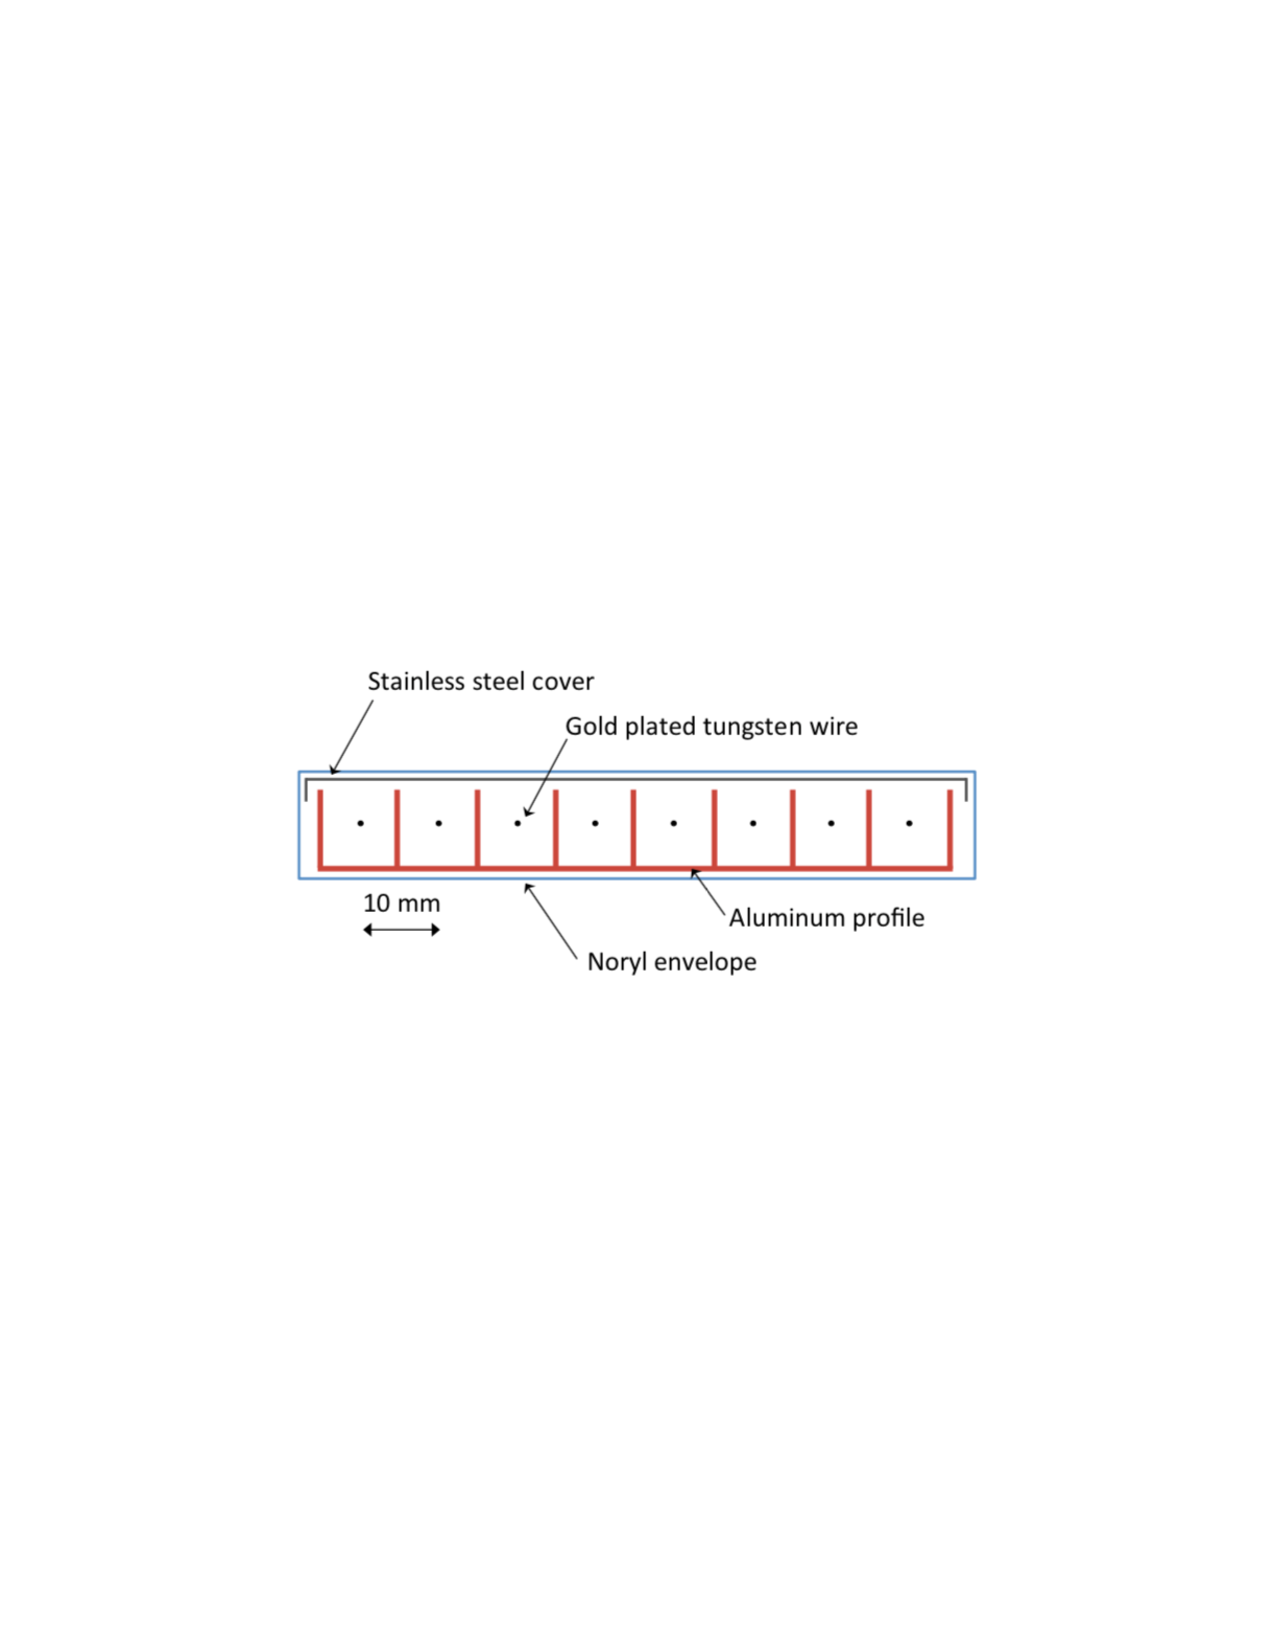
\includegraphics[width=0.45\textwidth, trim=5cm 12cm 5cm 10cm, clip]
                  {richwallMDT}
  \caption{The richwall mini drift tubes.  This image is taken
    from~\cite{ABBON201569}.}
  \label{fig::richwallMDT}
\end{figure}

The final type of large area tracking detector at COMPASS is the MWPC.  There
are 14 of these stations located throughout the experiment.  The MWPCs are
separated into three categories distinguished by the coordinates they measure.
The first type is called type A and consists of three projection views measuring
an x, u and v coordinate.  The second type is type A* and is the same as type A
but measures the y coordinate in addition to the other three coordinates.  Both
type A and A* have active areas of 178x120~cm$^2$.  The final type is type B
which has a smaller active area of 178x90~cm$^2$ and measures the same
projections as type A.  There are seven stations of type A, one station of type
A* and six stations of type B.  All three types have circular dead zones of
diameters 16~cm, 20~cm and 22~cm for types A, A* and B respectively. \par

The MWPCs operate on similar principles to the drift chambers but without a
calibration drift curve.  For this reason the MWPCs can be made to have one
common gas volume between each station.  Their position resolution is
determined as

\begin{equation}
\frac{\mathrm{sense \: wire \: separation}}{\sqrt{12}},
\end{equation}
\noindent
which is the variance of a uniform distribution.  The separation between sense
wires is approximately 2~mm which corresponds to a spacial resolution of these
detectors of around 600~$\mu$m.


\section{Particle Identification}
In the COMPASS spectrometer there are four types of detectors used to determine
particle identification (PID).  These four detectors are the ring image
Cherenkov (RICH) detector, electromagnet calorimeters (ECAL), hadron
calorimeters (HCAL) and muon walls (MW).  The RICH distinguishes between pions,
kaons and protons; ECAL1 and ECAL2 measure the energy from photons and
electrons; HCAL1 and HCAL2 measure the energy from hadrons; and MW1 and MW2
distinguish muons from all other particles.  The RICH, ECAL1, HCAL1 and MW1 are
in the large angle spectrometer in that respective order along the beam line.
The small angle spectrometer includes ECAL2, HCAL2 and MW2 again in that
respective order along the beam line. \par

The RICH detector operates similarly to the CEDARS, section~\ref{sec::addBeam}.
In the RICH, Cherenkov radiation is emitted from particles traveling through it
at an angle dependent on the particle's velocity.  The RICH is filled with a
dielectric gas, C$_4$F$_{10}$, which as an index of refraction greater than air.
The momentum of a particle going through the RICH is determined from bending
radius around SM1.  Therefore once the RICH determines the entering particles
velocity, the mass of particles can be distinguished.  A sketch of the RICH and
its operating principle is shown in Fig.~\ref{fig::rich}.  To distinguish
between particles, the minimum momenta are: 2.5~{\gvc} for pions, 9~{\gvc}
for kaons and 17~{\gvc} for protons.  The maximum momentum the RICH can
distinguish between any of these particles is 50~{\gvc}. This detector is
located in the large angle spectrometer before any calorimeters.\par

\begin{figure}[h!t]
  \centering
  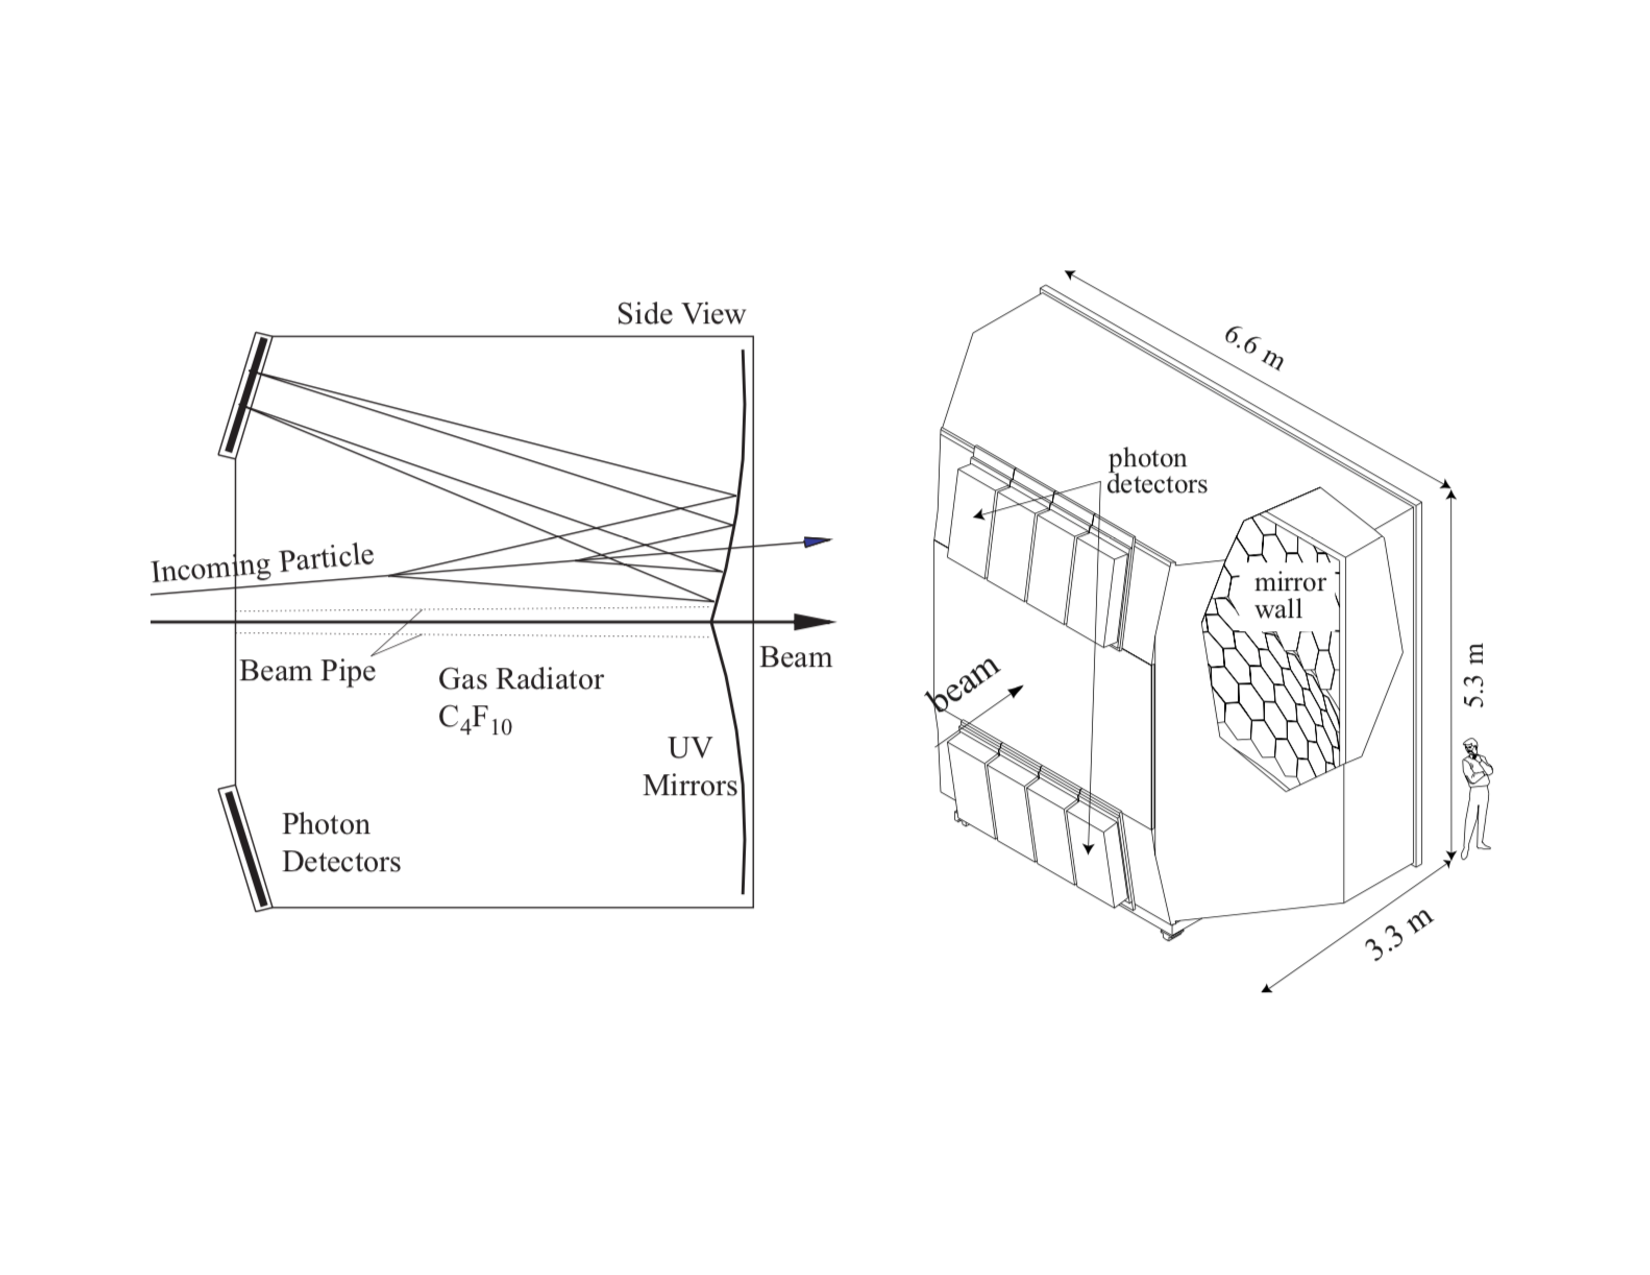
\includegraphics[width=0.6\textwidth, trim=1cm 5cm 1cm 4cm, clip]{rich}
  \caption{Side view demonstrating the principle of operation of the RICH
    detector.  This image was taken from~\cite{compassSpec}.}
  \label{fig::rich}
\end{figure}

The ECALs and HCALs both measure the energy of entering particles.  Both types
of calorimeters do this by stopping a specific entering particle, where the
amount of energy deposited in each respective calorimeter is proportional to the
incoming particle's energy.  ECALs are able to stop and measure electron and
photon energies and HCALs stop and measure hadron energies.  The energy
knowledge along with the momentum determined from the tracking detectors enables
the particle to be identified. \par

The ECALs are made of lead glass towers with photon multipliers attached to
these towers on one side.  An incoming photon or electron interacts with the
lead glass to produce a light signal, which is readout with these photon
multipliers.  Other particles also interact with the material in the ECALs
however hadrons and muons are able to exit through the detector unlike photons
and electrons.  A frontal view of ECAL1 is shown in Fig.~\ref{fig::ECAL1} and a
frontal view of ECAL2 is shown in figure Fig.~\ref{fig::ECAL2}. \par

\begin{figure}[h!t]
  \centering
  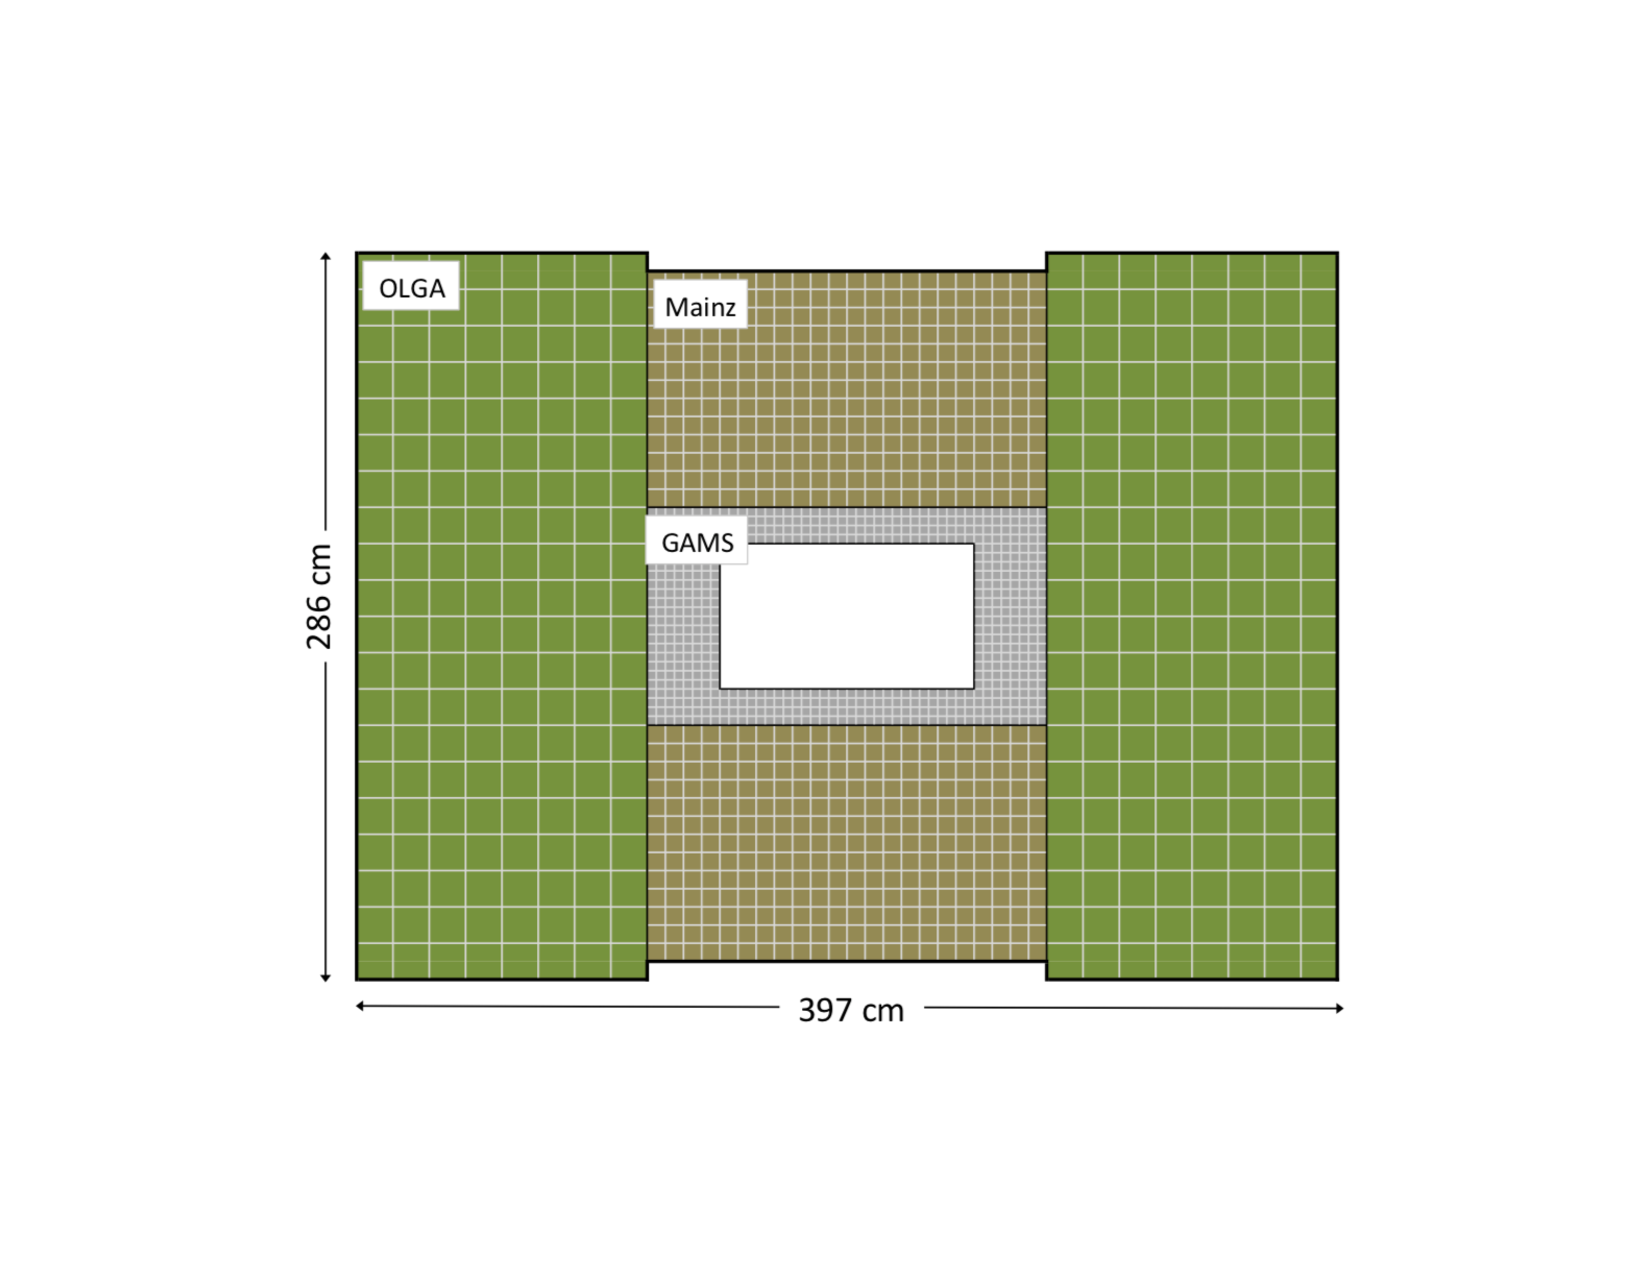
\includegraphics[width=0.6\textwidth, trim=4cm 4cm 4cm 4cm,clip]{ECAL1}
  \caption{Frontal view of the electromagnetic calorimeter 1.  This image is
    taken from~\cite{ABBON201569}.}
  \label{fig::ECAL1}
\end{figure}

\begin{figure}[h!t]
  \centering
  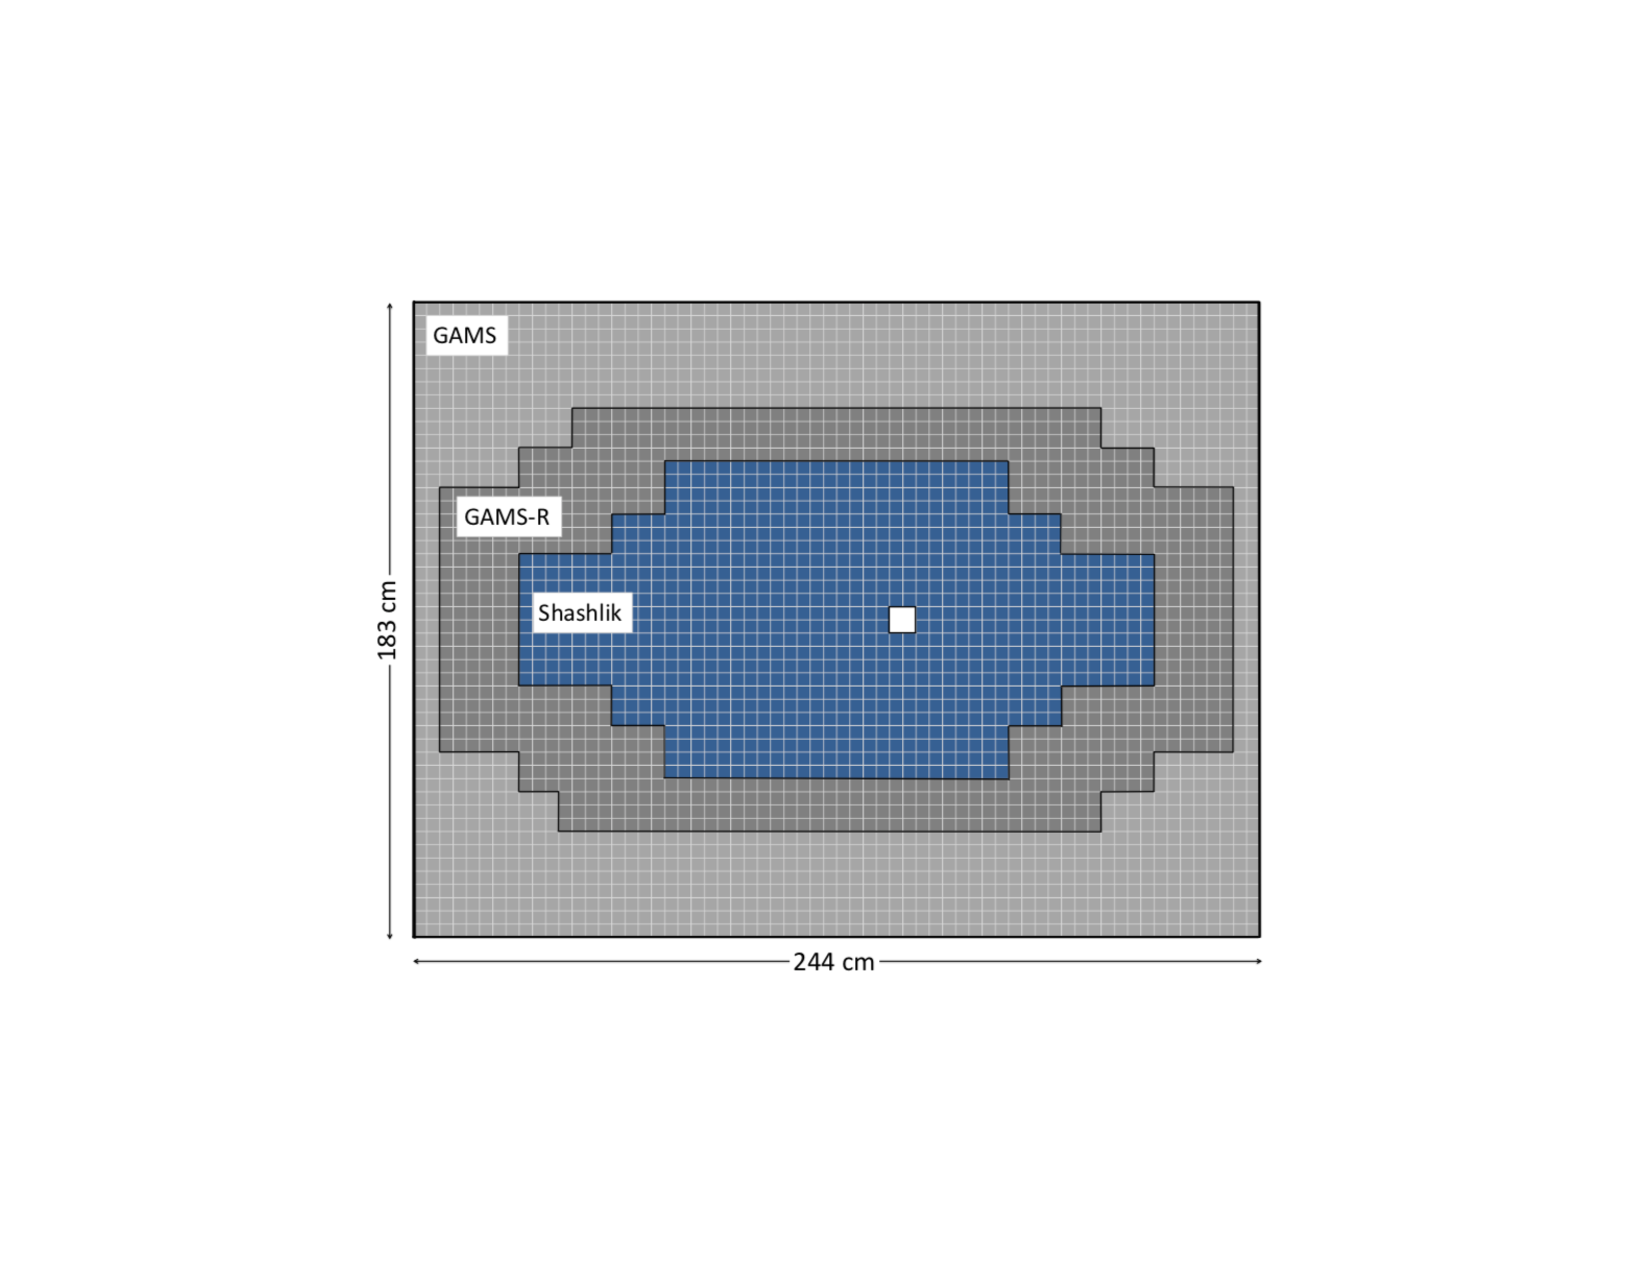
\includegraphics[width=0.6\textwidth, trim=4cm 4cm 4cm 4cm,clip]{ECAL2}
  \caption{Frontal view of the electromagnetic calorimeter 2.  This image is
    taken from~\cite{ABBON201569}.}
  \label{fig::ECAL2}
\end{figure}


The HCALs are sampling calorimeters, which are made of alternating layers of
iron and scintillating material.  An incoming hadron deposits all its energy in
the HCAL by making a particle shower in the iron.  This particle shower makes a
signal in the scintillating material, which is then read out by photo
multipliers.  The HCALs are placed after the ECALs in each stage of the
spectrometer because an electromagnetic shower happens within less material
budget than a hadronic shower.  The HCALs are effect at determining particle
energies from particle with energies between 10~GeV and 100~GeV. \par

The two MWs are located after an HCAL in their respective stages.  Due to their
higher mass and absence of color charge, muons are able to pass through the most
material budget of any of the particles detected at COMPASS.  For this reason
both MWs consist of an absorber and tracking detectors downstream of this
absorber.  Any particles that make it through the absorber are with a very high
probability muons. \par

MW1 consists of eight tracking planes before a 60~cm iron
absorber and the same number of tracking planes after this absorber.  The
tracking portions of MW1 are built similarly to the richwall, described in
section~\ref{sec::SAT}, in that they are also made of MDT modules.  The active
area of MW1 is 480x410~cm$^2$ and includes a dead zone of 140x80~cm$^2$.  Each
plane of this detector has a spacial resolution of 3~mm.  A sketch of MW1 is
shown in Fig.~\ref{fig::MW1}. \par

\begin{figure}[h!t]
  \centering
  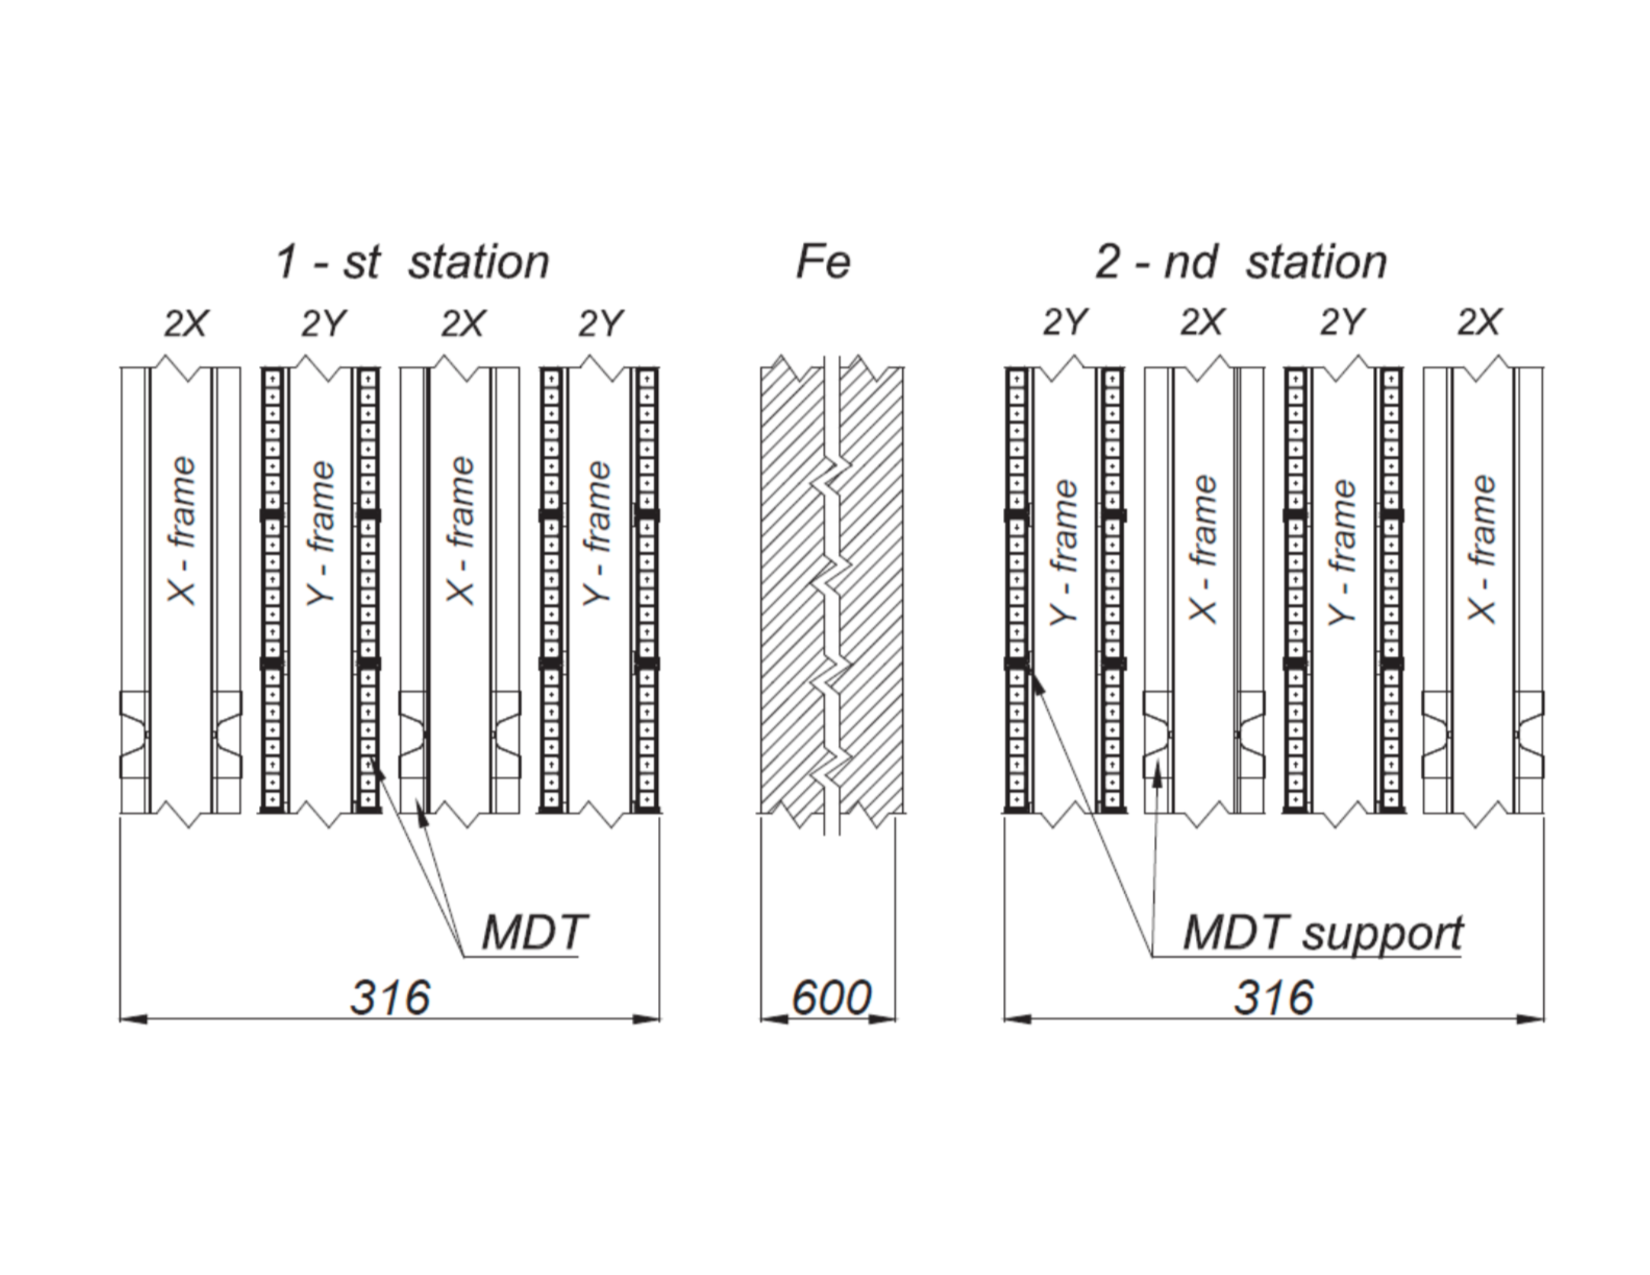
\includegraphics[width=0.7\textwidth, trim=1cm 3cm 1cm 3cm,clip]{MW1}
  \caption{A side view sketch of the muon wall 1 detector.  This image was taken
    from~\cite{compassSpec}.}
  \label{fig::MW1}
\end{figure}

The second muon wall, MW2, is located downstream of a 2.4~m thick concrete
absorber.  MW2 consists of 12 planes each with an active area of 450x450~cm$^2$
and a dead zone of 90x70~cm$^2$.  The detector operates similarly to the straw
detectors, section~\ref{sec::SAT}, in that the detector is made of drift tubes
with a wire in the center of these tubes.  The diameter of the drift tubes is
29~mm and the position resolution is about 1.4~mm. \par

There is one last absorber in the COMPASS spectrometer located before the H5
hodoscope at the end of the spectrometer hall.  This absorber is called muon
filter 3 (MW3) and ensures that the inner trigger is only triggered by a
muon. \par


\section{Trigger} \label{sec::trigger}
The trigger system at COMPASS defines what is an event.  Whenever the trigger
signal is given, all the detector information within a few nanosecond timing
window is recorded.  Due to the fact that there are very many background events
occurring as the beam impinges on the target, there is too much information
going to the front end modules (FEMs) of the detectors for the FEMs to process
and record all this information.  For this reason only a certain subset of all
the information is stored to disk.  The trigger system must therefore have good
timing resolution to make quick decisions on which data to record.  At COMPASS
the trigger systems consist of scintillating hodoscopes attached to PMTs.  The
timing resolution of these detectors is approximately 1~ns.  A top view
schematic of COMPASS showing where the relative positions of the hodoscopes for
each trigger is shown in Fig.~\ref{fig::TriggerElements}.  \par

\begin{figure}[h!t]
  \centering
  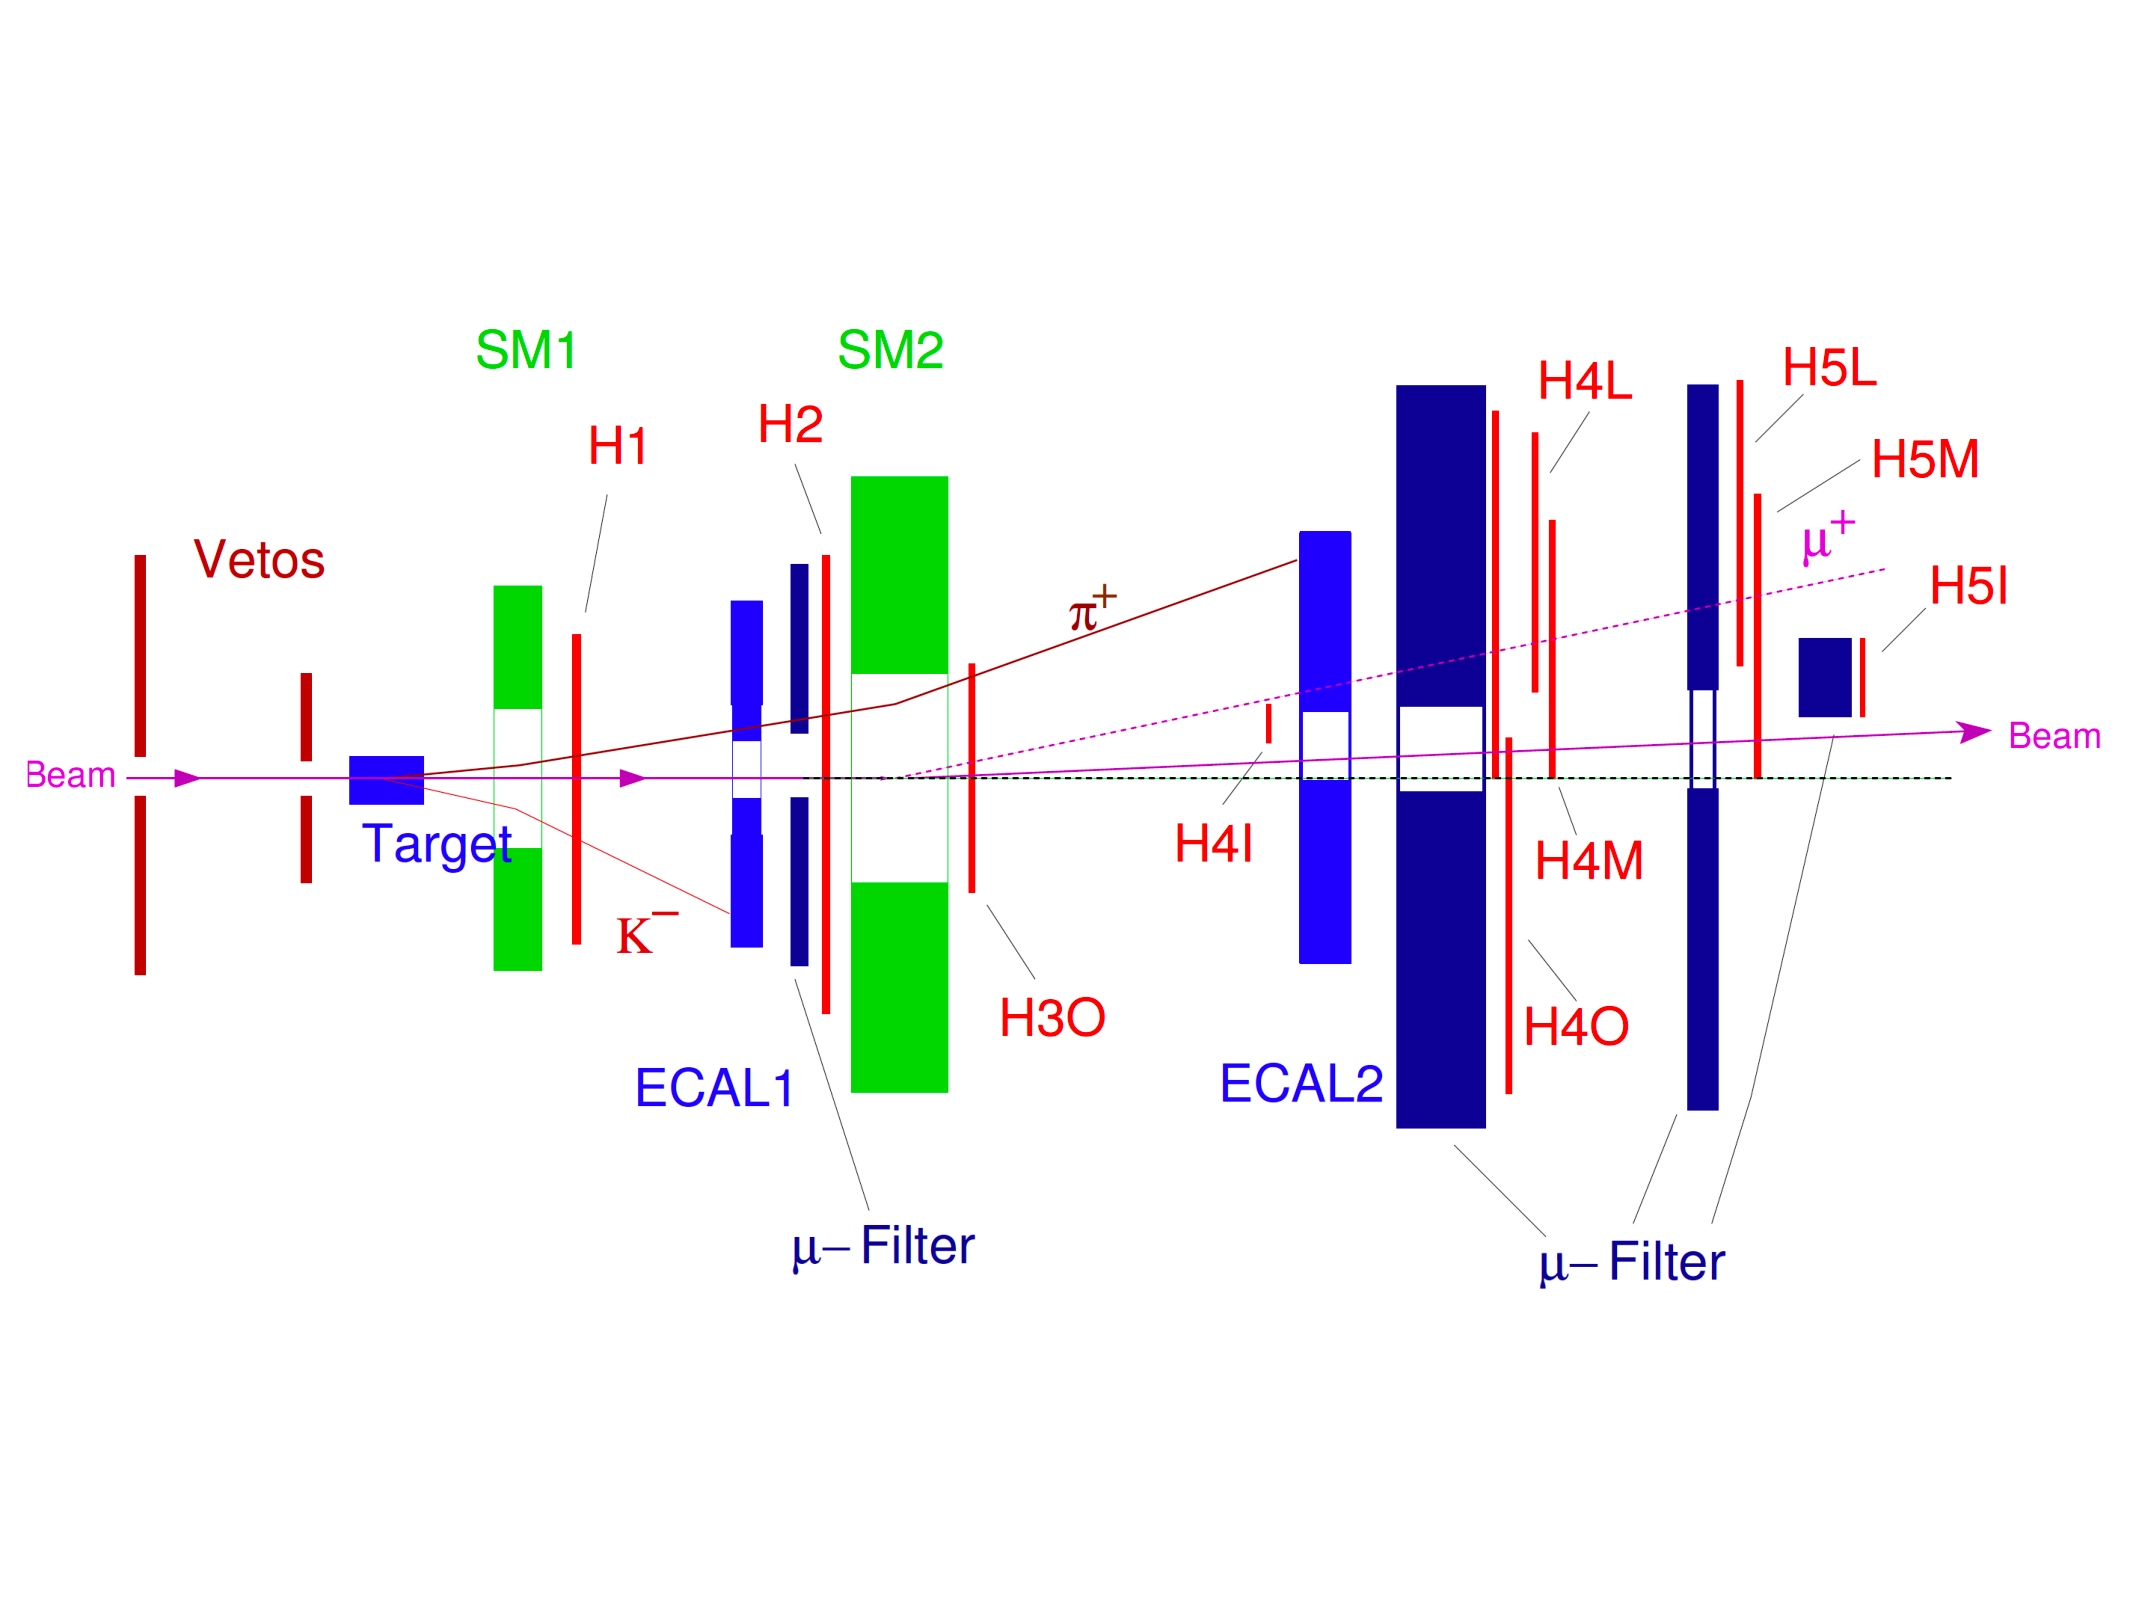
\includegraphics[width=0.9\textwidth]{TriggerElements}
  \caption{Top view of the spectrometer highlighting how different particles can
    signal a trigger.  This image was taken from~\cite{BERNET2005217}.}
  \label{fig::TriggerElements}
\end{figure}

At COMPASS there are five different triggers used to register physics events.
Each trigger type includes at least two hodoscopes at different z-positions in
the spectrometer.  The types of triggers are either target pointing, when the
hodoscope slabs are horizontal; or energy loss, when the hodoscope slabs are
vertical.  The target pointing trigger is setup and used with higher polar
scattering angles.  As the name suggest, this trigger signals when a particle is
scattered from the target.  The energy loss trigger is used to trigger on lower
Q$^2$ interactions and signals when a particle is bent a specified amount.
This concept is illustrated in Fig.~\ref{fig::TrigPrinc}.  \par

There are four triggers in SAS: the inner trigger (IT), the middle trigger (MT),
the ladder trigger (LT) and the outer trigger (OT).  The IT is an energy loss
trigger and includes the hodoscopes HI04X and HI05X.  The MT includes both
energy loss and target pointing slabs.  The hodoscopes in the MT are HM04X,
HM05X, HM04Y and HM05Y.  The MT hodoscopes whose names end with an X have
vertical slabs and those ending with a Y have horizontal slabs.  The LT is an
energy loss trigger which consists of HL04X and HL05X.  The final trigger in
SAS, the OT, is a target pointing trigger and consists of hodoscopes HO03Y and
HO04Y.  The remaining trigger system is in LAS and is a target pointing trigger
consisting of hodoscopes HG01Y and HG02Y.  The kinematic coverage for the 2015
triggers is shown in Fig.~\ref{fig::TrigCov6}. \par

\begin{figure}[h!t]
  \centering
  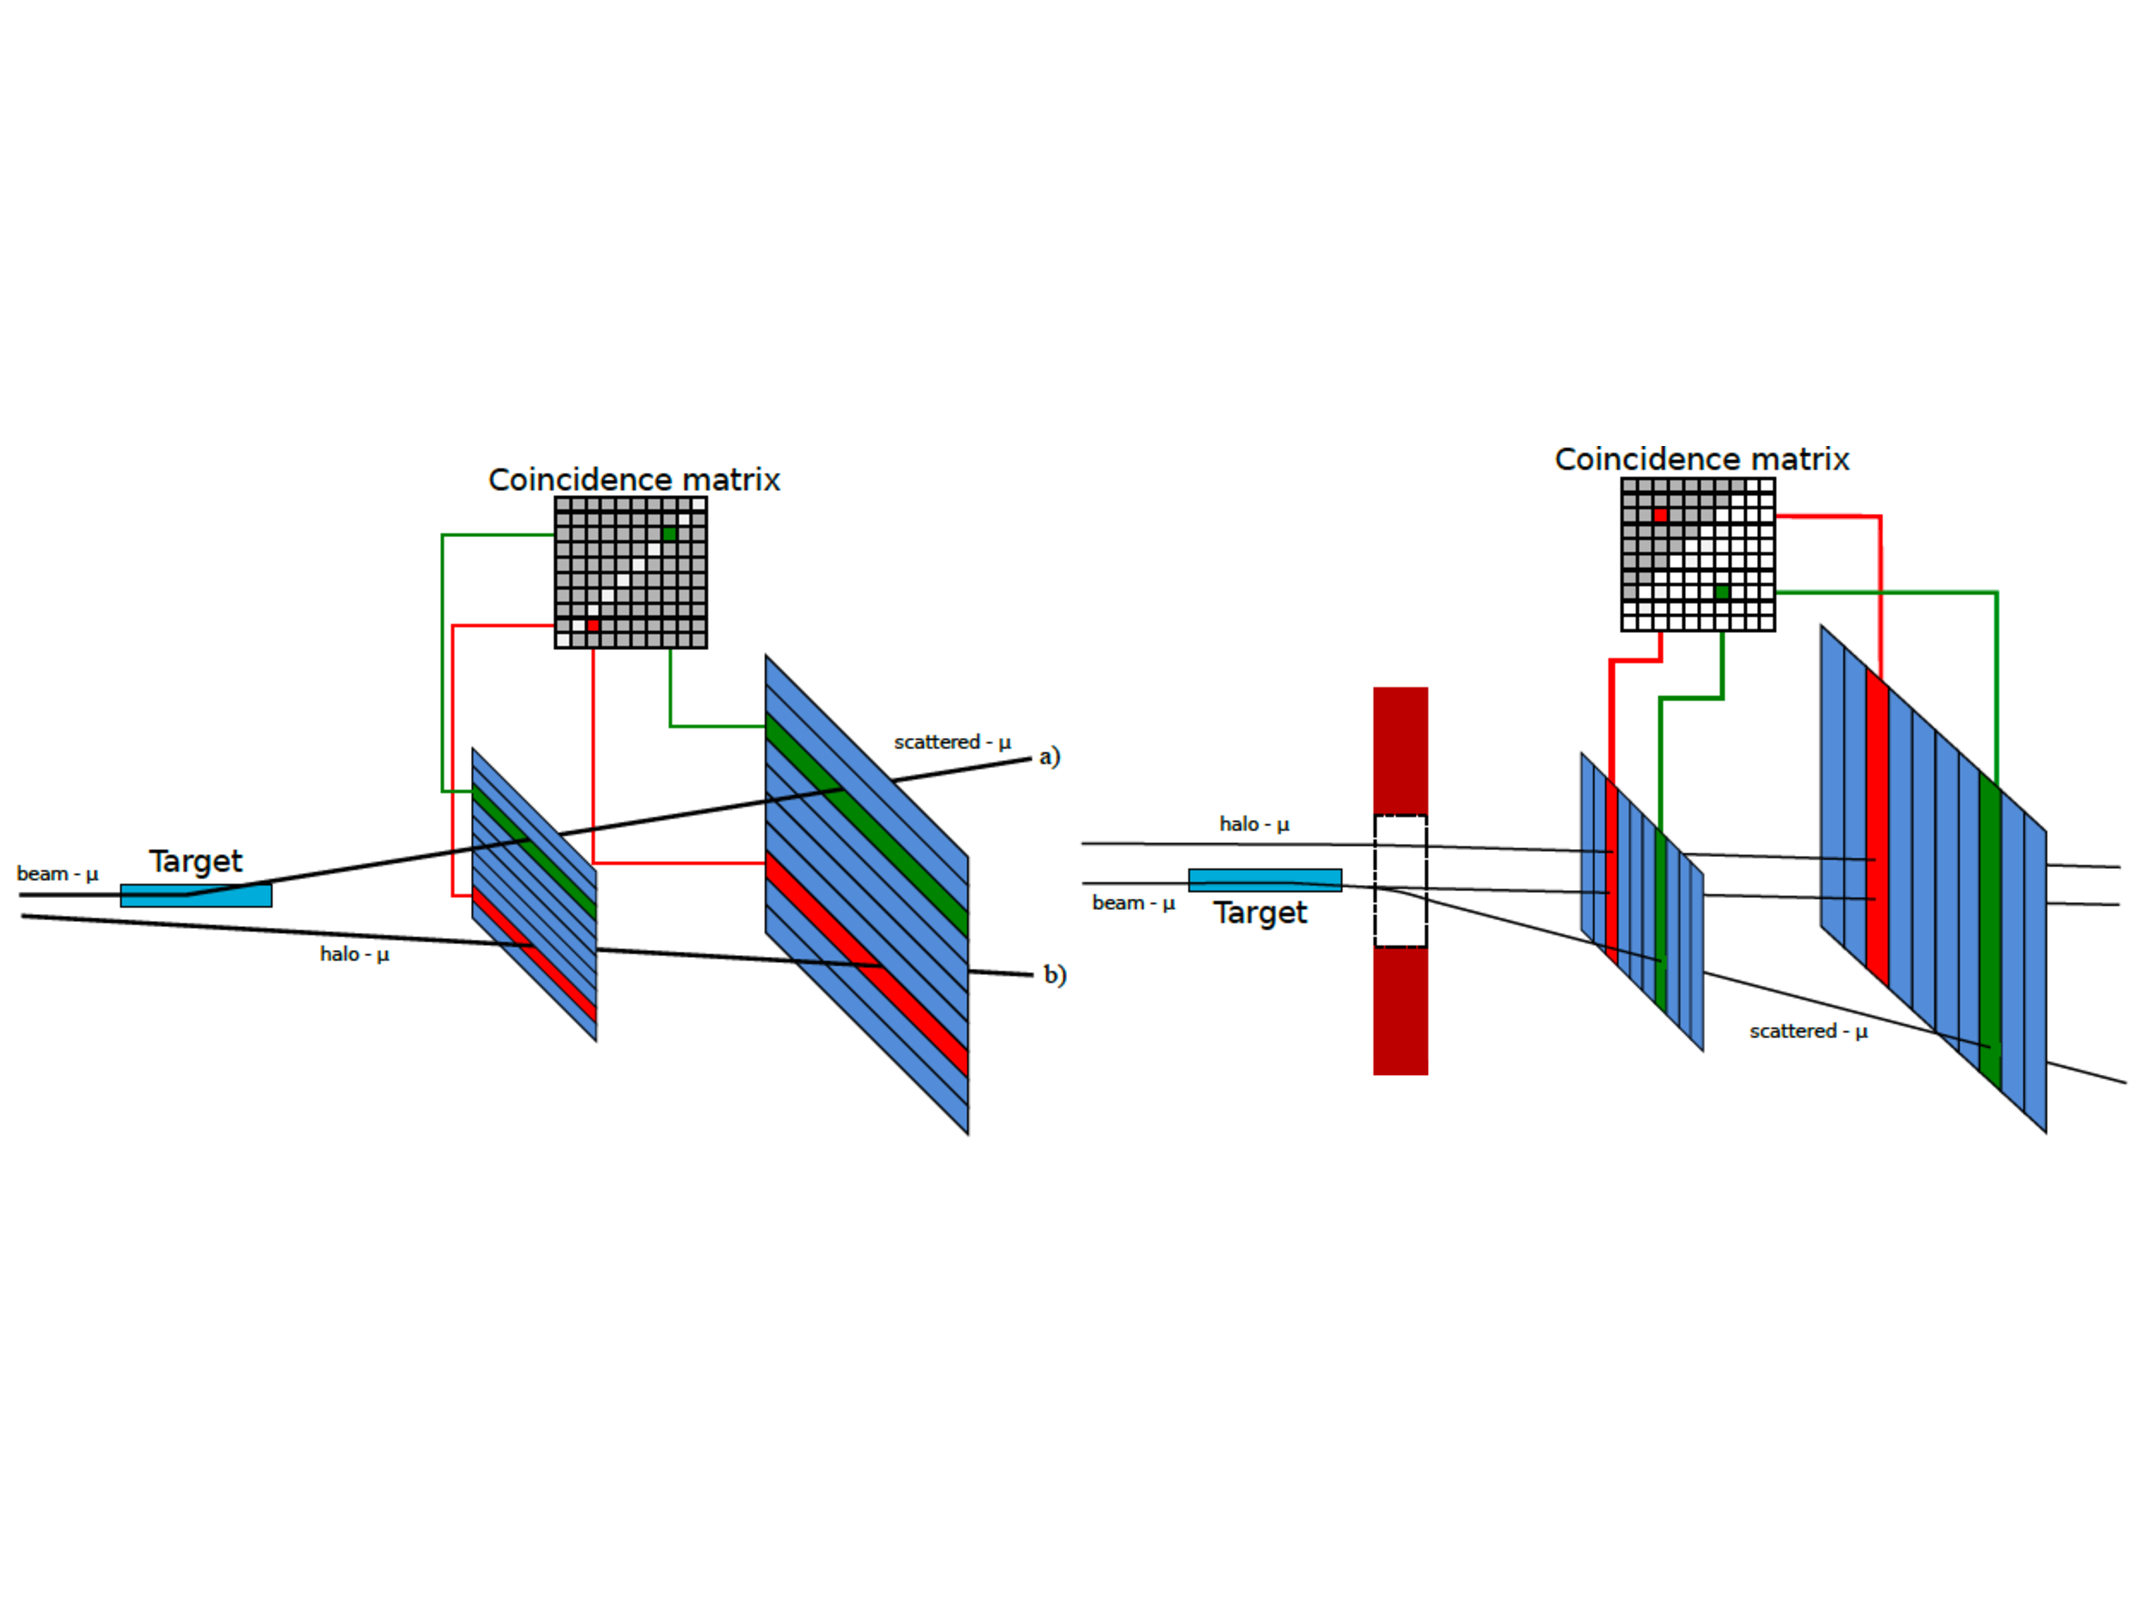
\includegraphics[width=0.9\textwidth]{TrigPrinc}
  \caption{The two types of triggers (left is target pointing and right is
    energy loss) at COMPASS and an illustration of the coincidence matrix used
    to select events of interest.  This image was taken from~\cite{trigDefs}.}
  \label{fig::TrigPrinc}
\end{figure}

\begin{figure}[h!t]
  \centering
  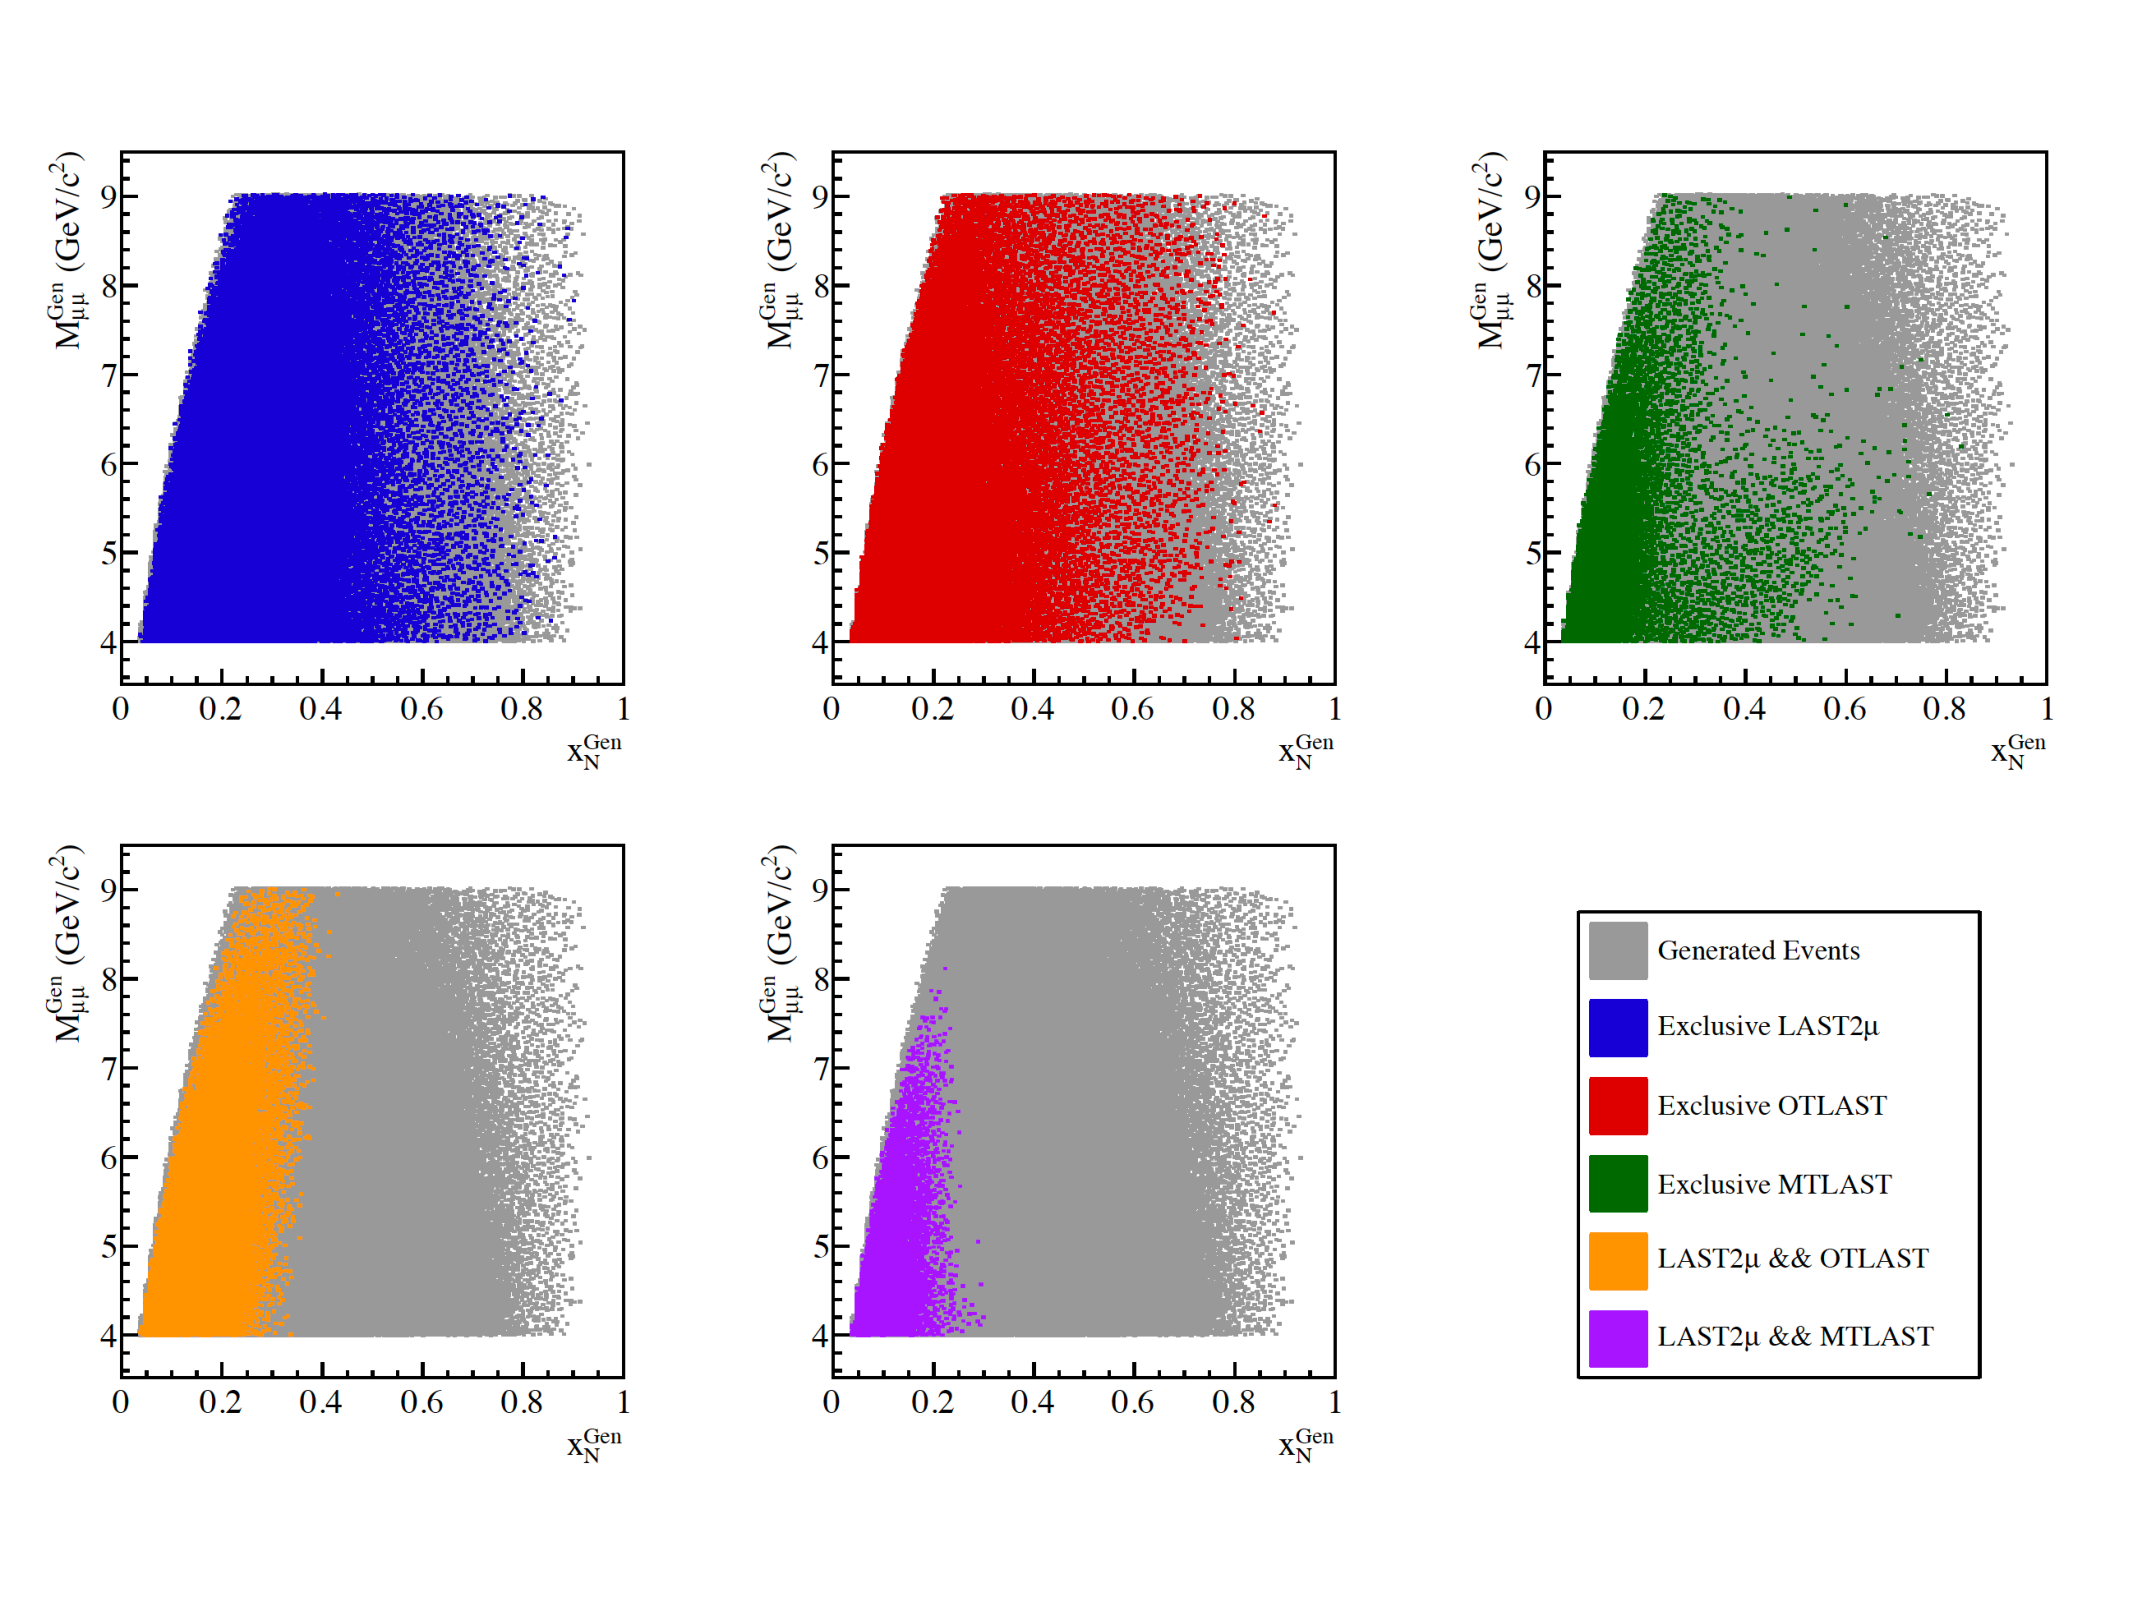
\includegraphics[width=0.9\textwidth]{TrigCov6}
  \caption{The kinematic coverage for the 2015 triggers determined from
    Monte-Carlo studies.  This image was taken from~\cite{longothesis}.}
  \label{fig::TrigCov6}
\end{figure}

In addition to signaling when interesting events occur, it is also import to
signal when background events are occurring.  For this reason there is also a
veto system upstream of the target as shown in Fig.~\ref{fig::TriggerElements}.
This veto trigger consists of hodoscopes attached to PMTs as well.  It is
centered on the beam axis but has a hole centered on the nominal beam line.  The
veto trigger is used to reject halo muons that surround the beam.  Halo muons
result from the beam decaying, as in Eq.~\ref{eqn::pionDecay} and
Eq.~\ref{eqn::kaonDecay}, where this decay occurs upstream of the target but
downstream of the ABS absorbers.  The muon halo surrounds the hadron beam due to
the muon's lower momentum, and it is for this reason that the veto hodoscopes,
outside of the beam line, are able to reject events that would occur due to the
halo.

There is one trigger in the spectrometer hall that is not a hodoscopes.  This is
the calorimeter trigger (CT).  The CT can be used as a trigger when a particle
deposits more than a certain energy threshold in the specified calorimeter.  In
2015 this trigger was only used as an independent study of the other triggers at
COMPASS. Particularly the CT was used to measure the trigger hodoscopes
efficiencies. \par

The last trigger used at COMPASS is a random trigger.  This trigger is setup
outside of the spectrometer area and registers a signal when a radioactive
source disintegrates.  In this way the random trigger is truly random.  In 2015
this trigger was used in studies of the beam flux.

In 2015, the goal was to measure two muons in the spectrometer.  For this
reason, two triggers must each signal a particle in coincidence for an event to
be registered.  For physics analysis the coincidence triggers are either two
muons in LAS (LASxLAS), one muon in LAS and one in the OT (LASxOT), or one muon
in LAS and one muon in the MT (LASxMT).  The LASxLAS trigger system covers the
high Q$^2$ and high x$_{\mathrm{beam}}$ phase space whereas the triggers
including a SAS hodoscope cover lower Q$^2$ values.  In addition to the dimuon
triggers there were three single muon triggers corresponding to a particle in
detected in LAS, MT or OT.  These three single muon triggers, however, where
pre-scaled down to record only one of every 500, 100 or 100 events respectively.
For further tests, 2015 included a random trigger and a beam trigger pre-scaled
down by 35000.


\section{Data Acquisition}
The data acquisition (DAQ) collects data from the over 250,000 detector channels
and transfers this data to storage on magnetic tape at CASTOR (CERN Advanced
STORage).  Despite the triggering system used to reduce the data rate, the data
still is recorded at event rates between 10~kHz to 100~kHz.  A typical COMPASS
event size is 45~kB.  The DAQ is designed to process these data rates and size
while minimizing the dead time associated with data collection and transfer. In
2015 the dead time was approximately 10\%.  The total data the DAQ recorded,
after the spectrometer finished commissioning, was approximately 820~terabytes
of raw data. \par

Data collection begins with the digitization of information from a detector
channel.  This digitization is performed by a time-to-digital converter (TDC) or
an analogue-to-digital converter (ADC). These TDCs and ADCs are either on the
detector FEMs or on custom COMPASS readout electronics named: GANDALF (Generic
Advanced Numerical Device for Analog and Logic Functions), GeSiCA (Gem and
Silicon Control and Acquisition) or CATCH (COMPASS Accumulate Transfer and
Control Hardware).  After digitization the data is transferred by optical fibers
to an FPGA multiplexer where the data is buffered by spill and arranged by
event.  From there an FPGA switch sends the data to multiplexer slaves.  The
slaves are online computers that oversee the final steps for raw data and
transfer this data to CASTOR.  

\section{Data Reconstruction}\label{sec::dataReconstruction}
The COMPASS Reconstruction and AnaLysis Program (CORAL) reconstructs the raw
data into physical quantities.  For example CORAL is able to convert the raw
data into particle tracks with momentum, charged and possibly an originating
vertex location~\cite{CORAL}.  The raw data from the DAQ is digitized timing
information from tracking detectors or digitized energy information for
calorimeters.  The process of reconstructing tracks takes the detector timing
information and determines a position in space for a particular tracking
detector based on a calibration.  CORAL then uses a Kalman Filter to determine
straight tracks in regions with no or low magnetic field~\cite{KalmanFilter}.
The tracks are then connected through the magnetic field using a fast lookup
table for known possible bending radii.  At this point a track is determined to
have a momentum, charge and an associated $\chi^2$ value.  From there the tracks
are extrapolated back to the target region and the intersection of at least two
tracks is determined as a vertex.  If in addition to the two intersecting
tracks, a beam particle can be extrapolated forward to the same vertex location
then the vertex is assigned to be a primary vertex.  Otherwise the vertex is
defined as a secondary vertex.

This reconstruction stage reduces the data volume by approximately a factor of
10.  In 2015 there were several data reconstructions performed.  Between each
reconstruction improvements were made to detector calibrations, detector
alignment, beam tracking and any other preprocessing improvements that could be
made.  The final two productions are the t3 production and the slot1 production.
The results shown in this thesis are from either t3 or slot1 productions.  The
slot1 production was the last production.  The difference between t3 and slot1
production is a new beam telescope reconstruction algorithm and an optimized
alignment which a new detector descriptions.  Specifically the hodoscopes for
triggers were changed to be described a detector split in half as oppose to a
detector split in fourths.  The changes between t3 and slot1 resulted in a 10\%
increase in events.

After reconstruction has been performed the data is stored in data structured
trees (DSTs).  The usual procedure of reconstruction which gives physical values
such as momentum and charge to tracks, results in data called miniDSTs.  There
is also the possibility to save more information, for example detector hit
location information, to make so-called fatDSTs.  These DSTs are in a format
which can be processed by PHAST (PHysics Analysis Software Tool).  PHAST is a
COMPASS program written to further analyze physics data.  With PHAST there is
the possibility to loop over all the miniDSTs and make certain kinematical cuts
and to produce so-called $\mu$DSTs based on these cuts.  In 2015 $\mu$DSTs were
made for all the analysis data where a cut was applied to the miniDSTs saving
only events with at least two muons.  Both CORAL and PHAST are fully
object-oriented C++ programs. \par

\subsection{Monte-Carlo Production}
Monte-Carlo data is simulated data which is performed in three steps.  First a
programs generates specific physics processes based on their theoretical
probabilities.  The generators of Monte-Carlo used for this thesis are PYTHIA
versions 6 and 8~\cite{pythia}.  Next a GEANT4 simulation of COMPASS determines
if a detector will register a hit from these generated physics processes.  This
saves the data in a raw data format which can be reconstructed by CORAL.
Finally the simulated data is reconstructed by CORAL and analyzed in PHAST the
same as if the data were real data. \par


\section{2015 Drell-Yan Data Taking} \label{sec::compass_2015_dy_setup}
The 2015 Drell-Yan data taking is one of the main programs for the COMPASS-II
experiment.  The data taking began in April of 2015 and ended in November of
that year.  The physics data used for analysis started in July and finished at
the end of data taking.  The data recorded before July was used for calibrations
and commissioning.  The total analysis data was split into nine data periods
labeled W07-W15 where each data period corresponded to approximately two weeks
of beam time. The spin orientation of each target cell was reversed after the
first sub-period of every period to reduce systematic effects arising from
different geometric acceptances and luminosities of the up and downstream target
cells. \par

\subsection{Hadron Absorber}
The previous sections in this chapter described the spectrometer setup generally
and mentioned the specifics for the 2015 setup.  The main unique hardware
addition in 2015 is the hadron absorber.  The hadron absorber was installed
because the beam intensity is high and results in many main strong interactions
in the target.  For this reason the first tracking detectors upstream of SM1
have occupancies that are too high for a satisfactory tracking performance.
Therefore the hadron absorber was installed to prevent all particles except
muons from entering the spectometer. \par

The hadron absorber was placed just downstream of the two target cells as can be
seen in Fig.~\ref{fig::Habs}.  The absorber corresponded to approximately 7.5
interactions lengths of material, where the material was mostly alumina
(Al$_2$O$_3$) and concrete.  Inside the absorber was an aluminum target followed
by a tungsten plug, each of radius 2.5 cm.  The tungsten was used as a beam
dump, while the aluminum was present to prevent back scattering from the
tungsten beam plug.  A side view showing the dimensions and materials used can
be seen in Fig.~\ref{fig::Abside}.  Both the aluminum target and tungsten plug
served the double purposes as absorbers and also as unpolarized nuclear targets.
In addition to the hadron absorber two 3~mm thick $^6\mathrm{Li}$ absorbers were
added just downstream of the primary absorber to absorb thermal neutrons
produced in the primary absorber.  This $^6\mathrm{Li}$ absorber was proposed to
improve the performance of the first tracking detector downstream of the target
even with the hadron absorber installed. \par

\begin{figure}[h!t]
  \centering
  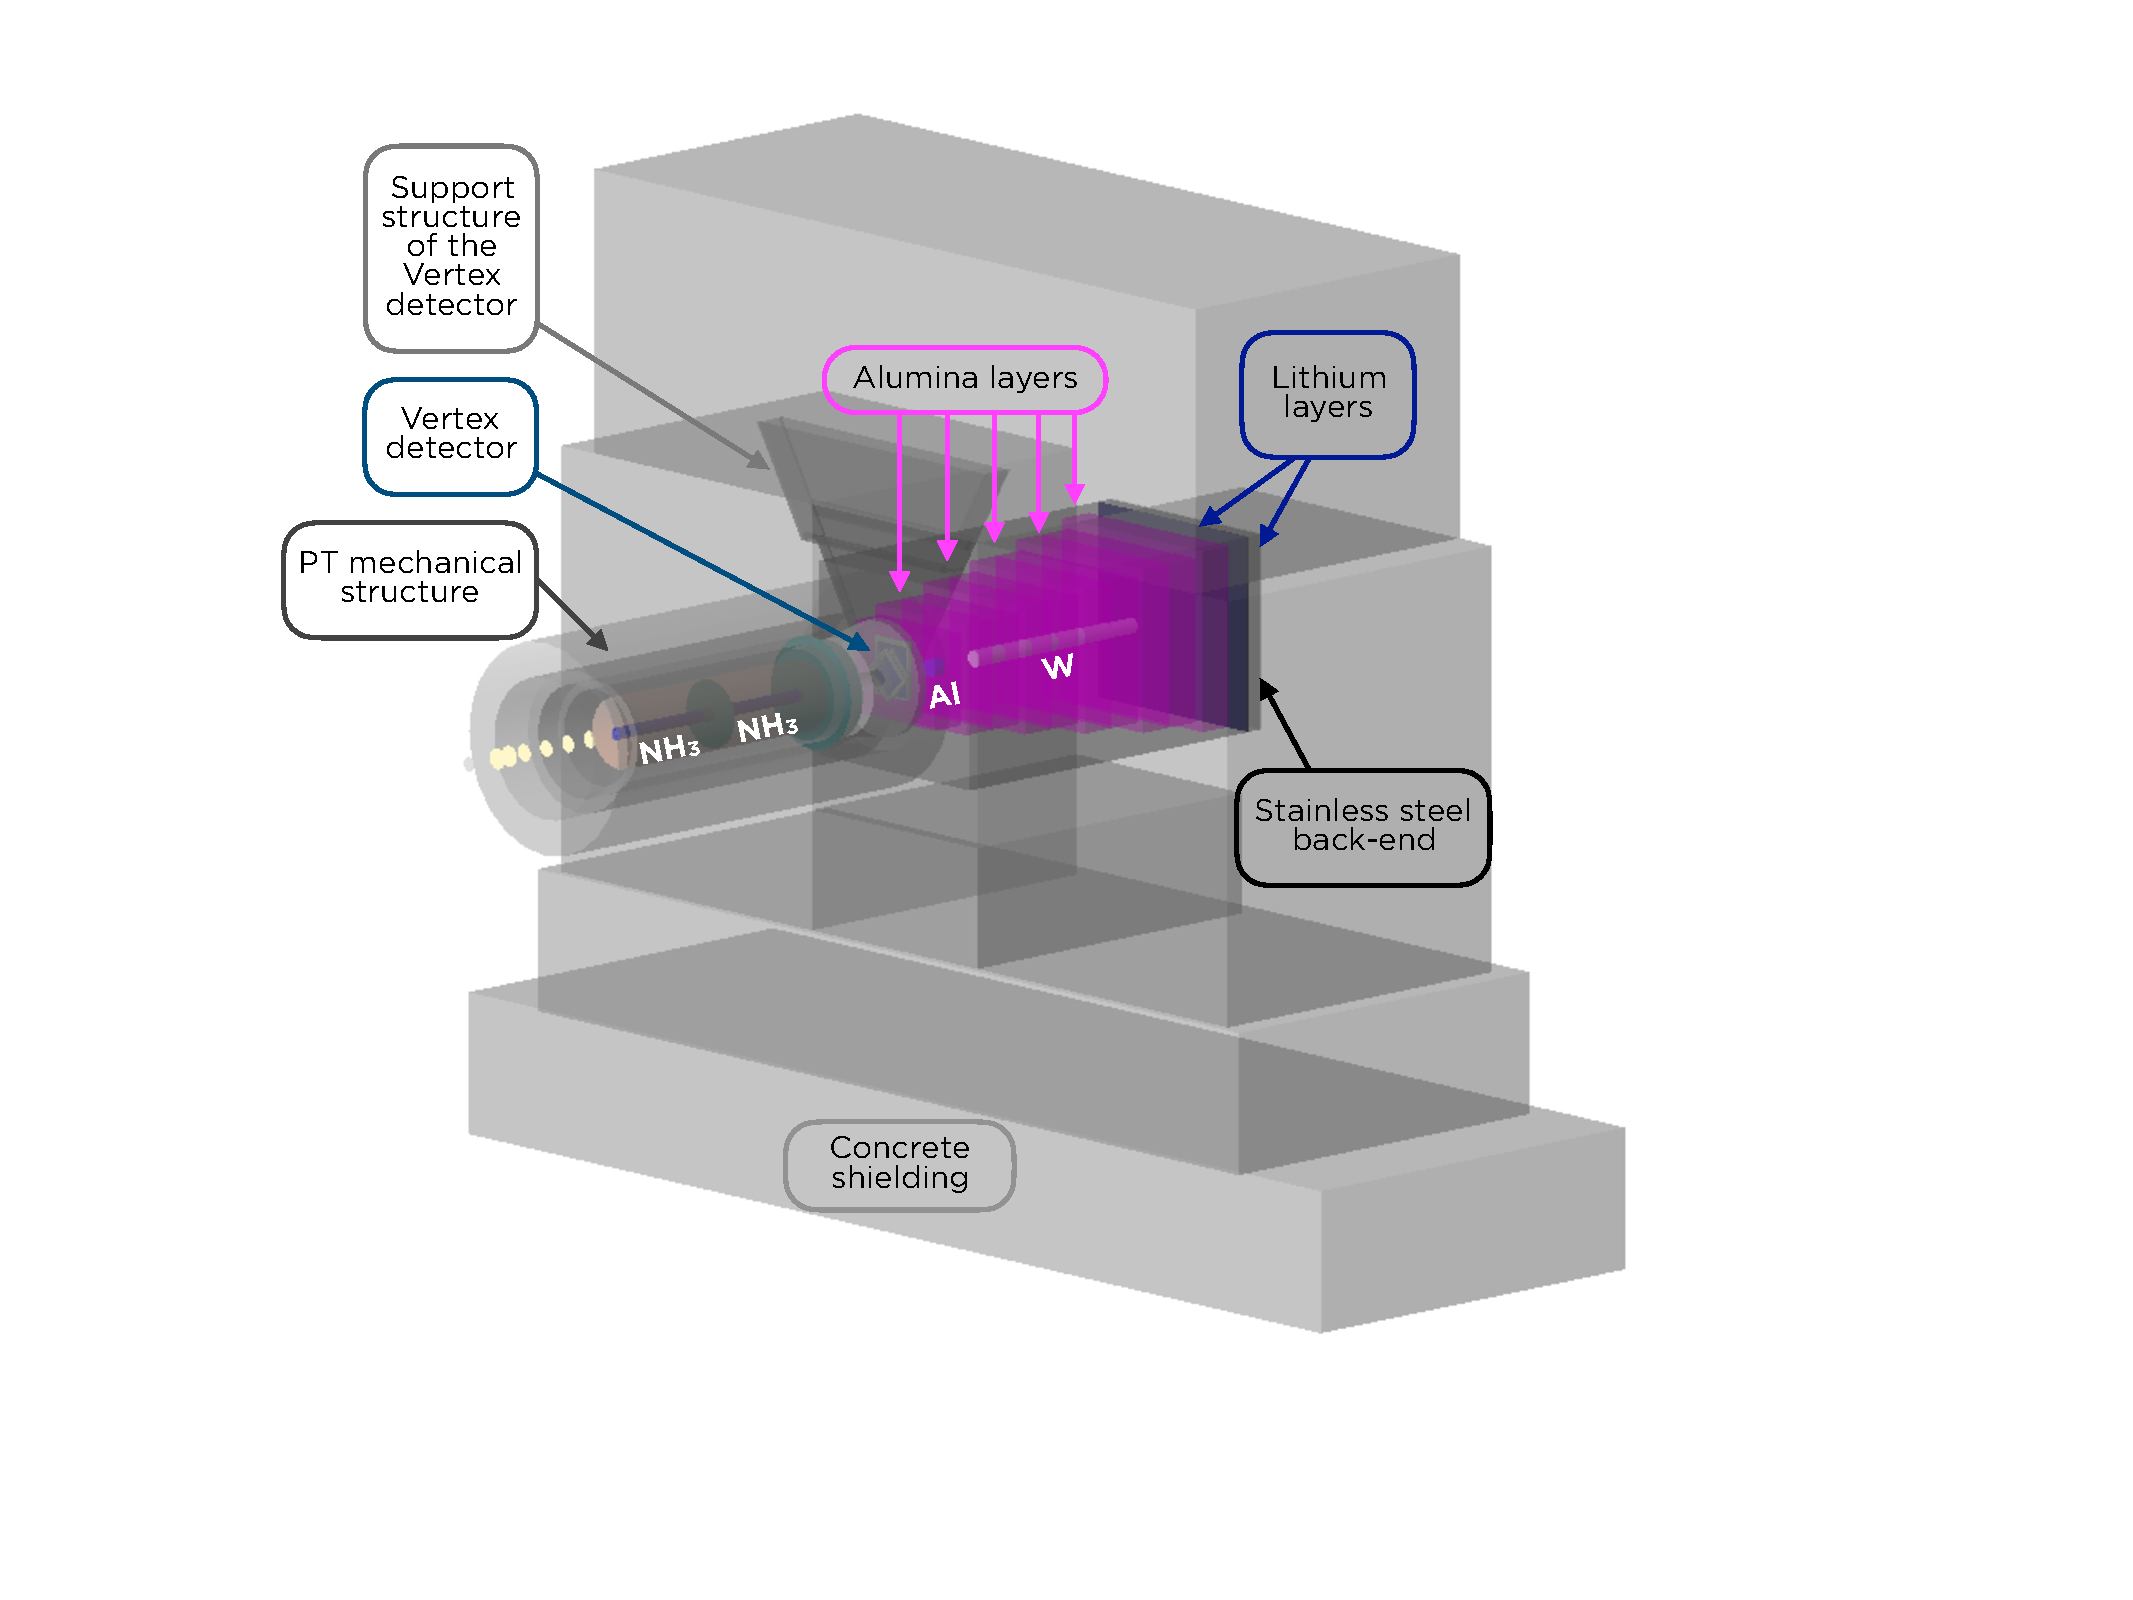
\includegraphics[width=0.6\textwidth]{Habs}
  \caption{The hadron absorber downstream of the polarized target in 2015.  This
    image was taken from~\cite{longothesis}.}
  \label{fig::Habs}
\end{figure}

\begin{figure}[h!t]
  \centering
  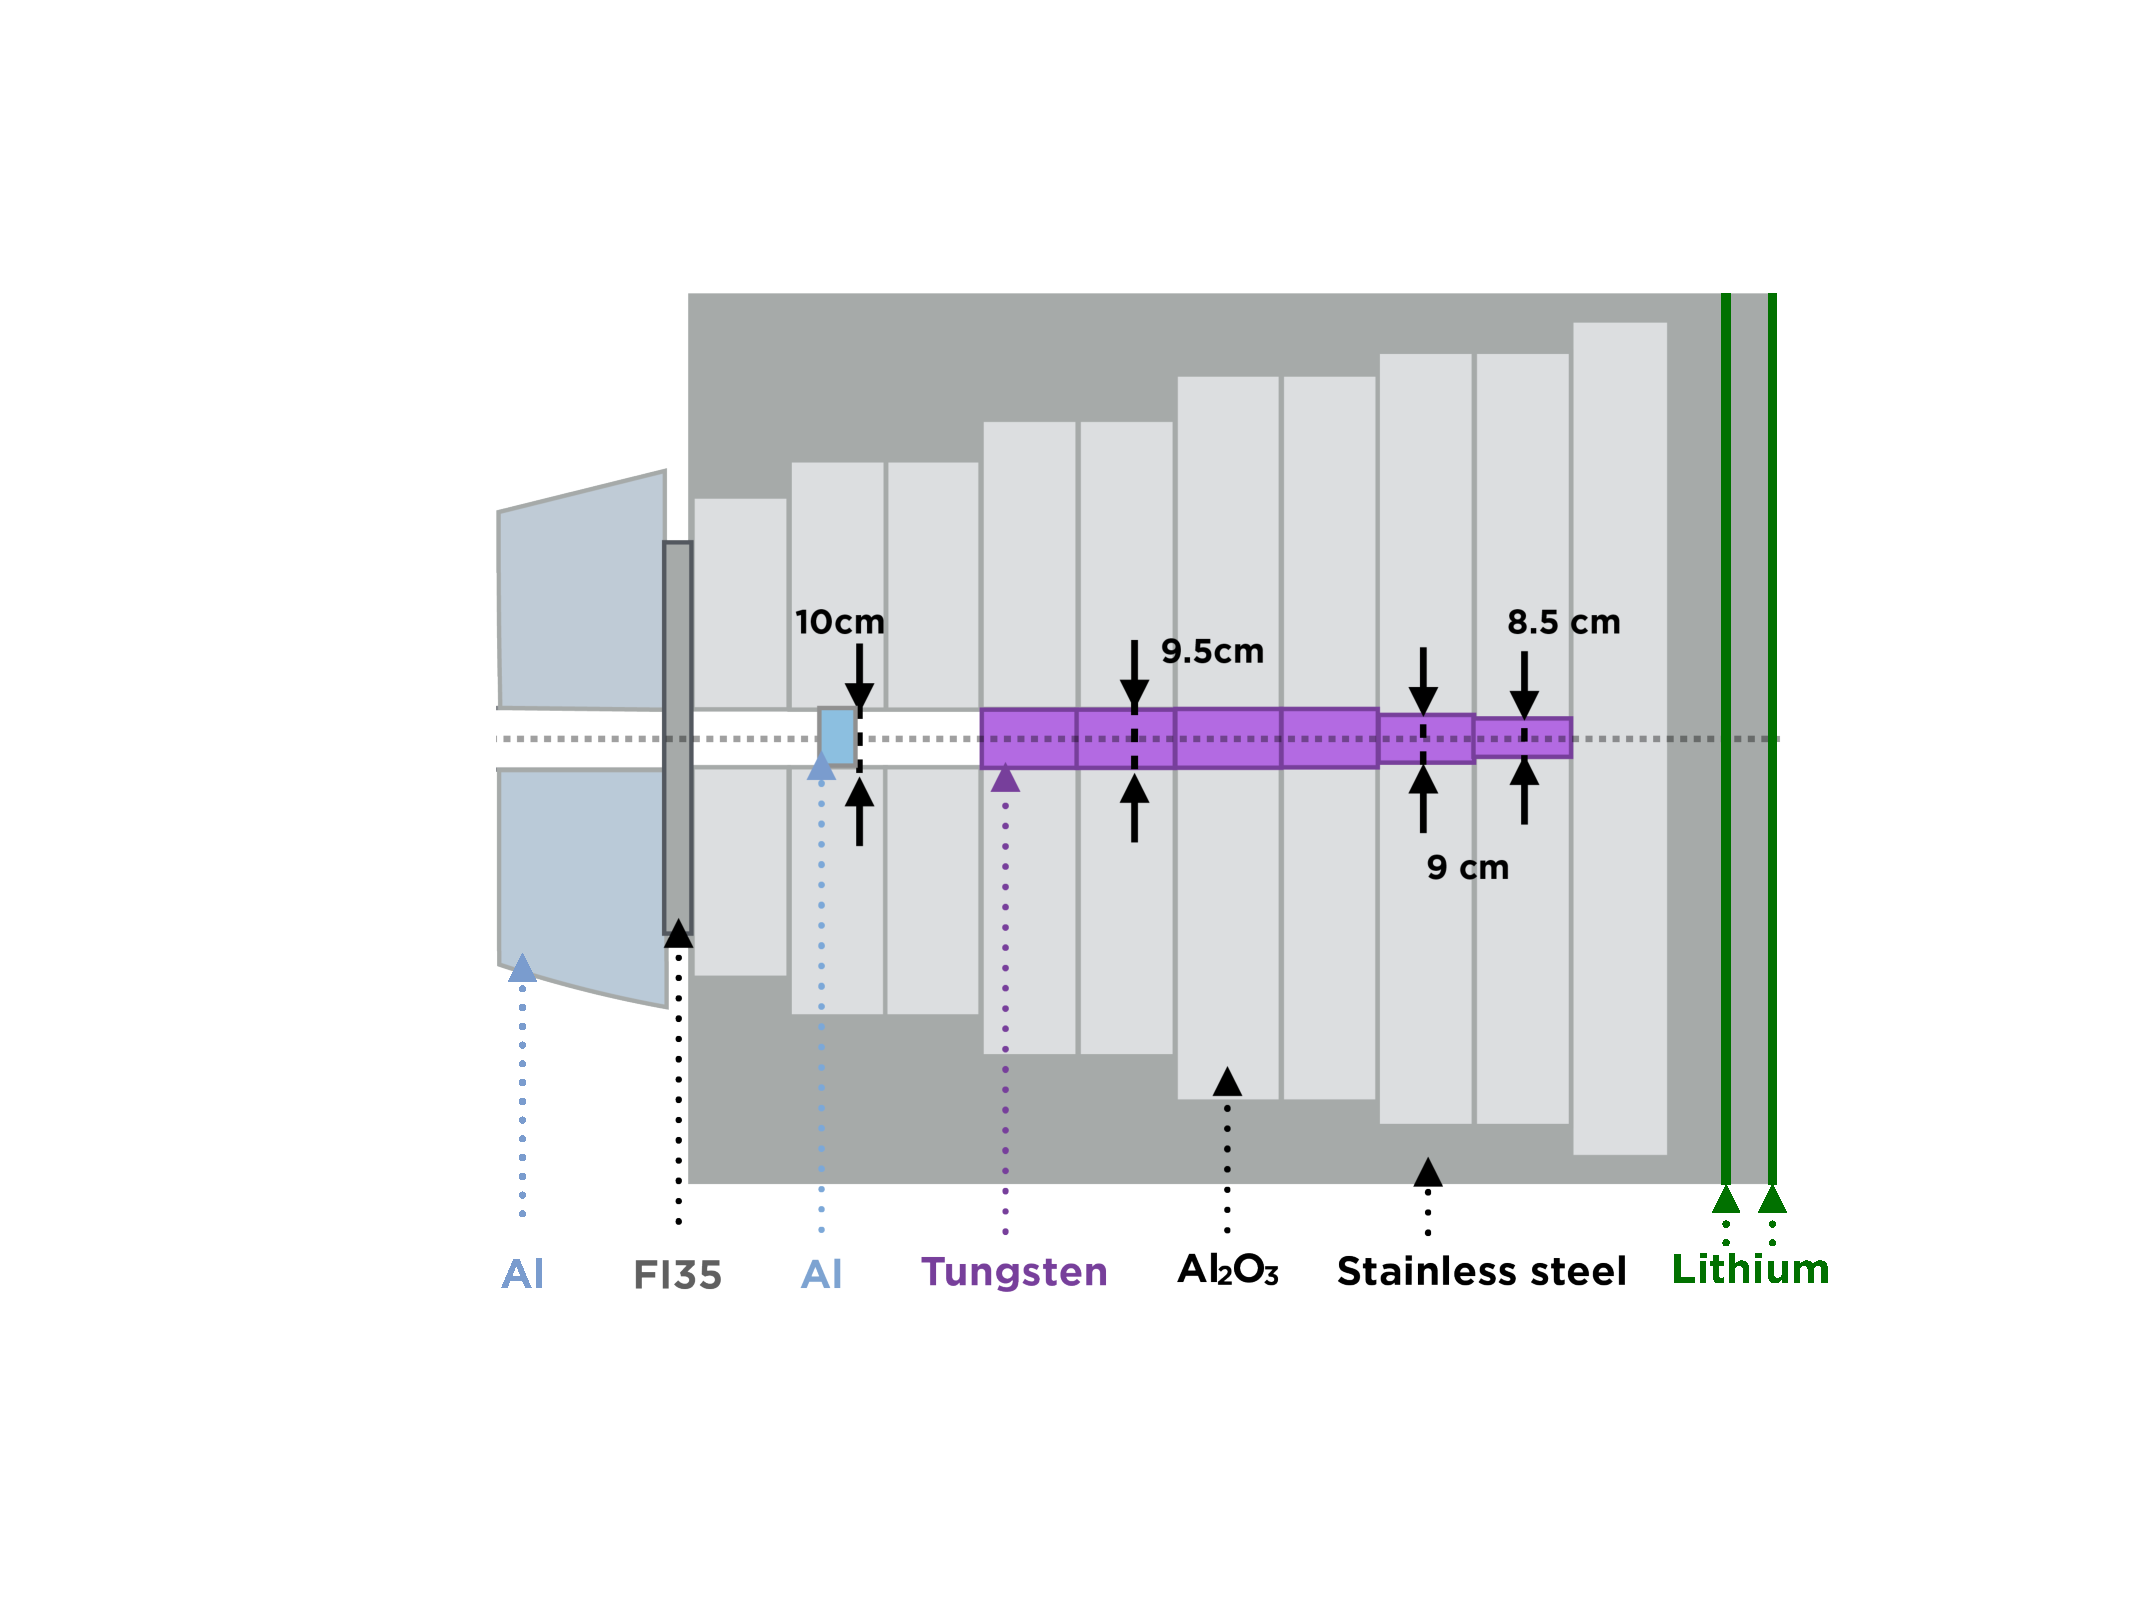
\includegraphics[width=0.6\textwidth]{Abside}
  \caption{Side view of the hadron absorber used in 2015.  This image was taken
    from~\cite{longothesis}.}
  \label{fig::Abside}
\end{figure}

\chapter{Drift Chamber 05} \label{ch::dc05}
\ifpdf
\graphicspath{{Chapters/DC5/Figs/Raster/}{Chapters/DC5/Figs/PDF/}{Chapters/DC5/Figs/}}
\else \graphicspath{{Chapters/DC5/Figs/Vector/}{Chapters/DC5/Figs/}}
\fi

Drift Chamber 05 (DC05) is a large-area planar drift chamber.  It was
constructed in 2014 and 2015 at the University of Illinois and Old Dominion
University and was then shipped to CERN for final assemble.  DC5 was installed
to the large angle spectrometer of COMPASS during the spring of 2015.

The DC5 detector is an import tracking detector, which successfully collected
data from 2015 through 2018 and will continue to be an important component for
track reconstruction in future measurements.  The author of this thesis helped
with the construction at Illinois and the assembly at CERN and as well for
performing calibrations and maintaining DC5.


\section{Motivation for Drift Chamber 05}

Simulations of the COMPASS spectrometer for Drell-Yan measurements determined
that 96\% of all events include a track in the large angle
spectrometer~\cite{proposal}.  For this reason the Drell-Yan trigger system was
designed only to record events with at least one track in LAS.  As DC5 was
installed in LAS it is therefore very important in track reconstruction for
Drell-Yan measurements.  Additional simulations with the Drell-Yan setup and
this corresponding COMPASS Drell-Yan trigger showed that the global
reconstruction efficiency drops below 30\% without DC5 and half of another large
area tracker in LAS~\cite{quintans_rec_march12}.  That is to say the
spectrometer reconstruction efficiency is very poor without DC05 and half of
another LAS large area trackers which has unstable performance.
Fig.~\ref{fig::standardRec} and Fig.~\ref{fig::withLARec} show the nominal
global reconstruction efficiency and the worst case scenario for Drell-Yan
measurements respectively.  For these reasons it was very important to have DC05
installed and working reliably.

\begin{figure}[h!t]
  \centering
  \begin{subfigure}{.5\textwidth}
    \centering 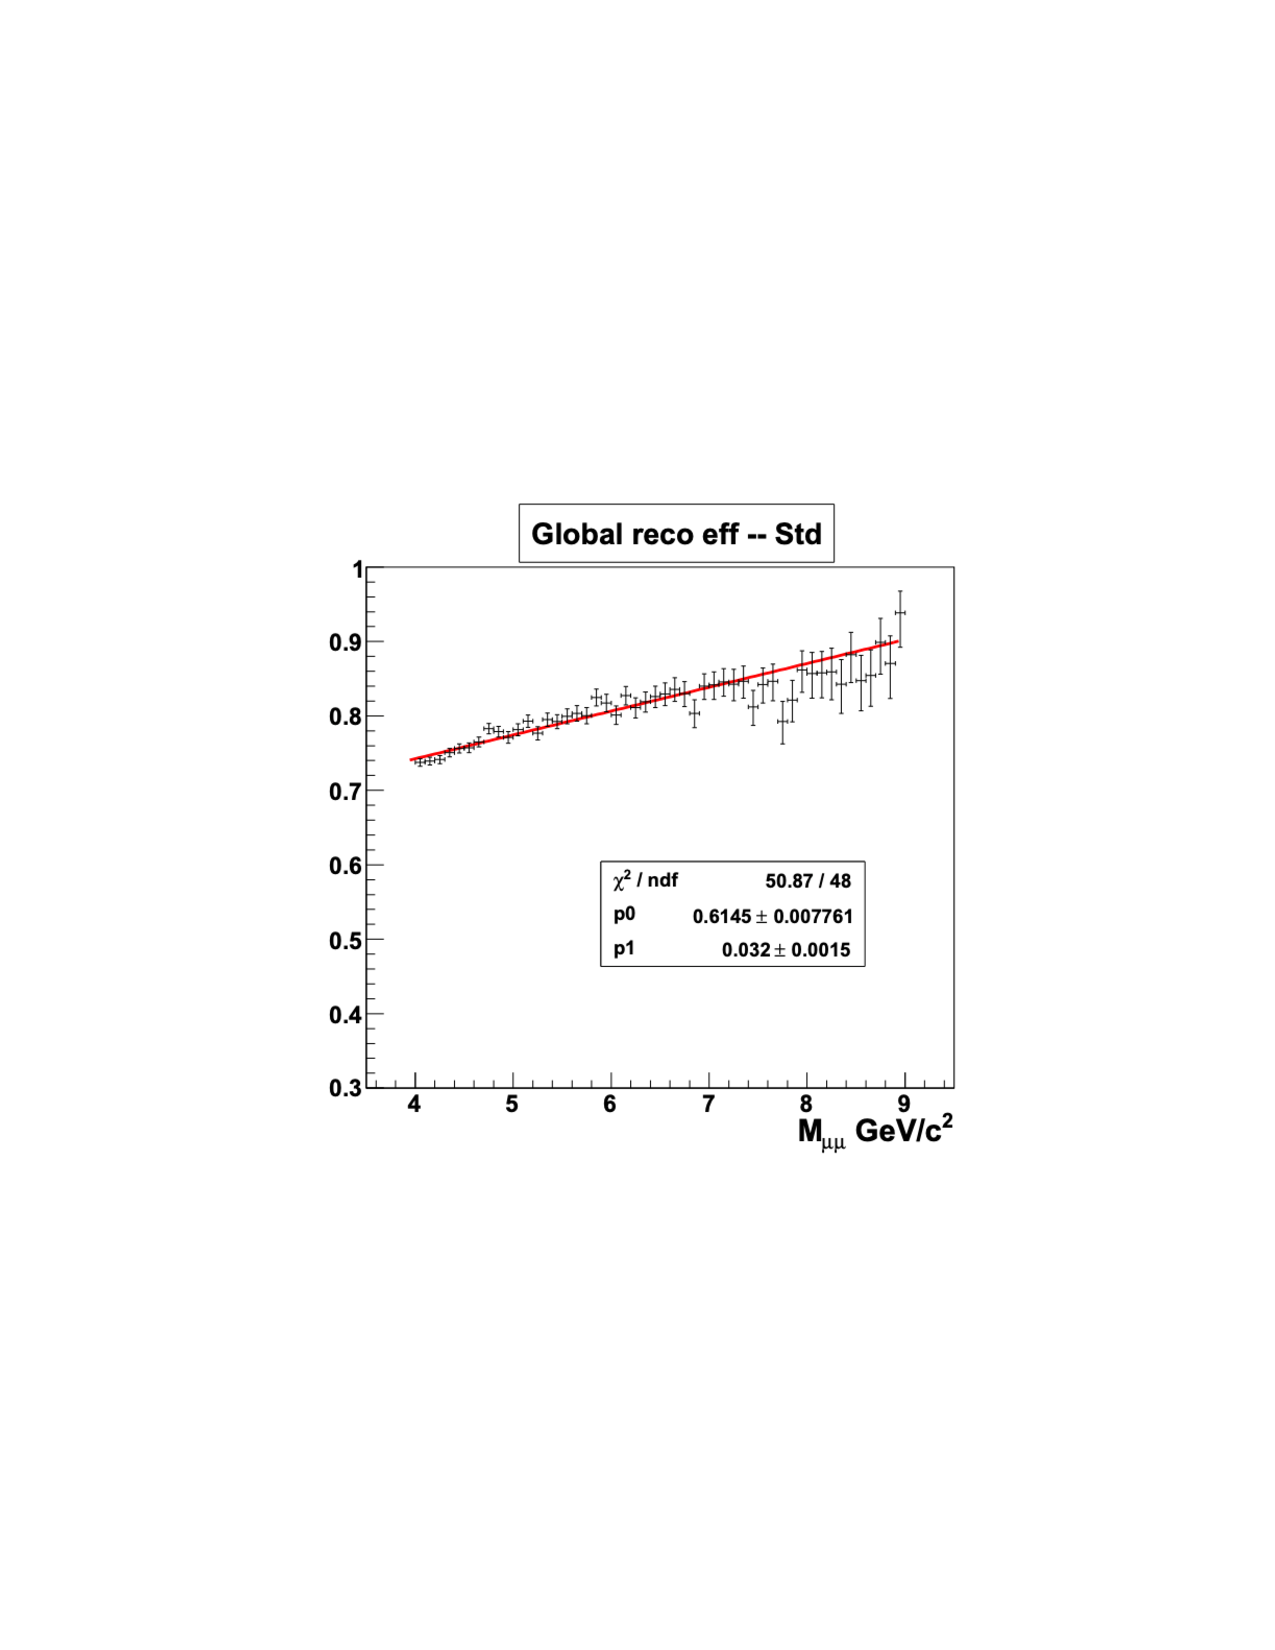
\includegraphics[width=\linewidth, trim=5cm 8cm 5cm 8cm,
      clip]{standardRec}
    \caption{Global reconstruction efficiency with all detectors working.  This
      image was taken from~\cite{quintans_rec_march28}}
    \label{fig::standardRec}
  \end{subfigure}%
  \begin{subfigure}{.5\textwidth}
    \centering
    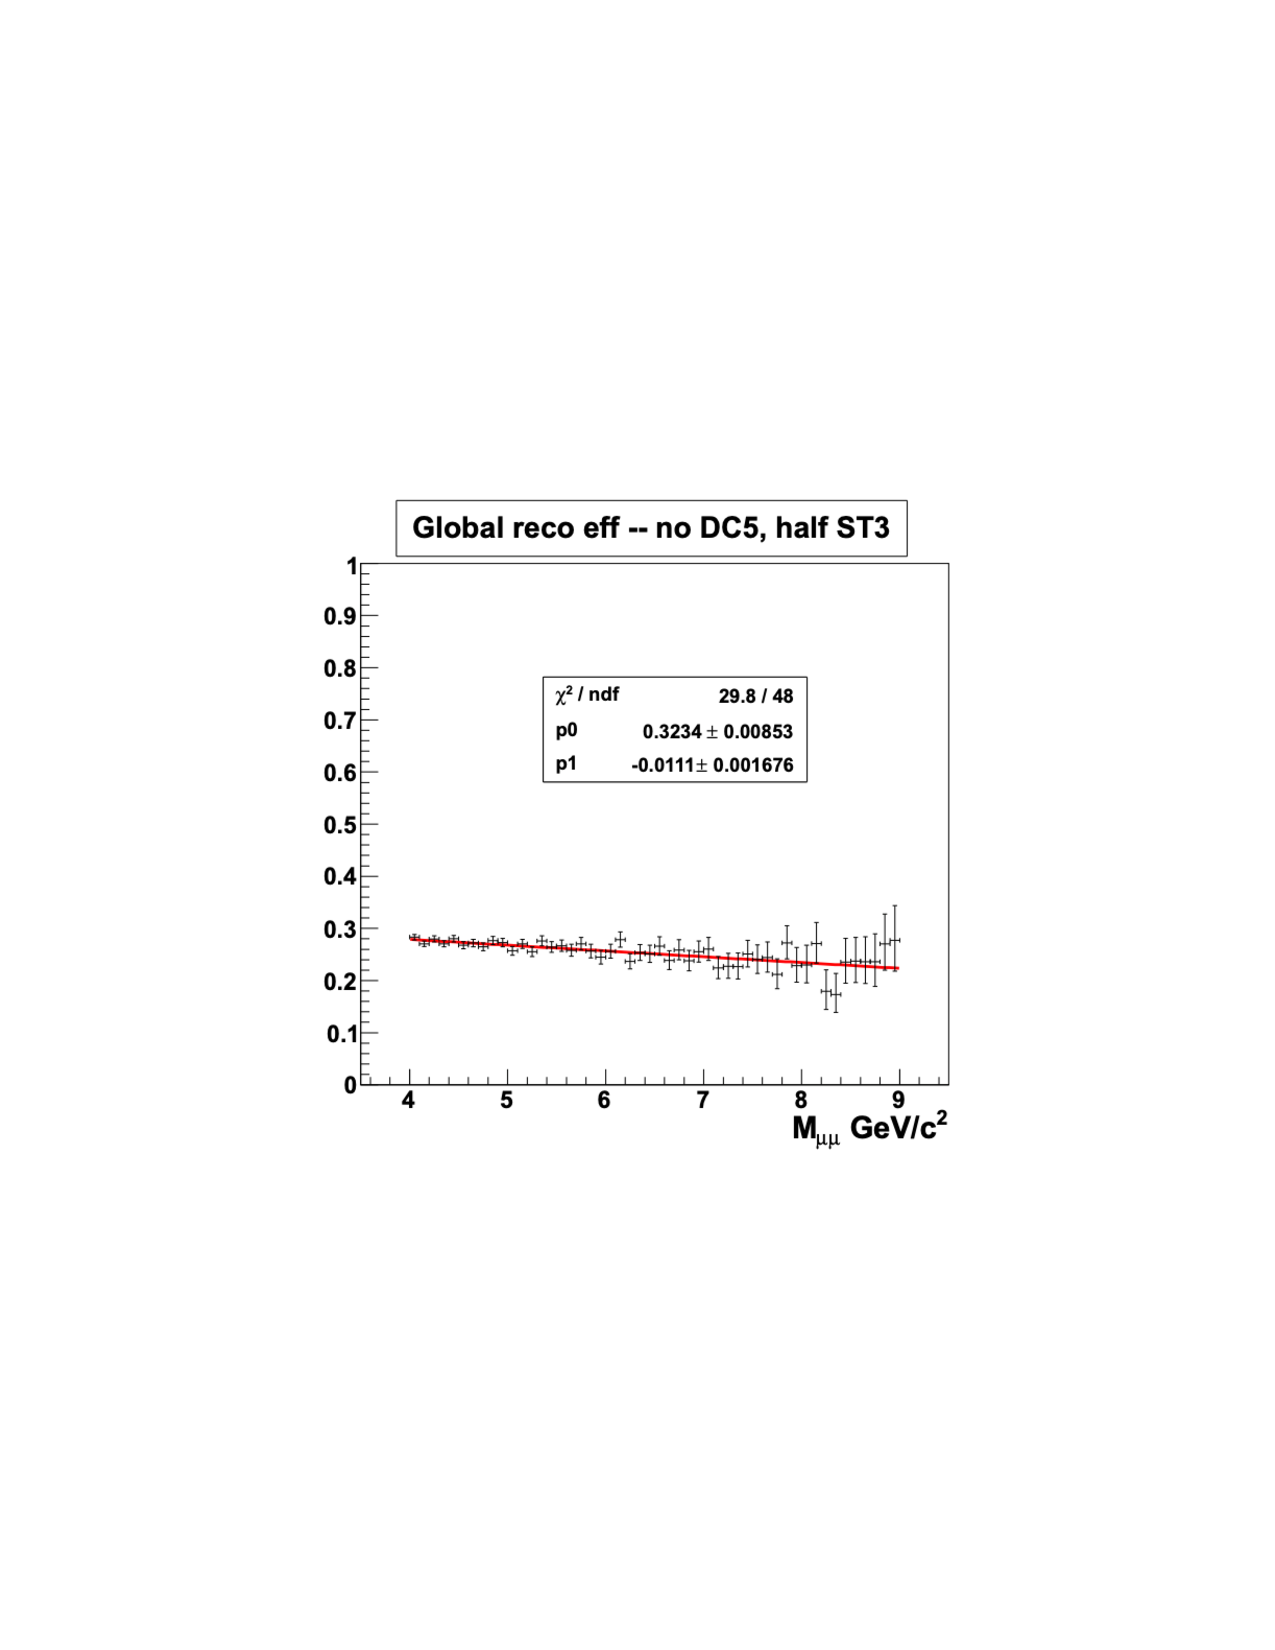
\includegraphics[width=\linewidth, trim=5cm 8cm 5cm 7.5cm, clip]{withLARec}
    \caption{Global reconstruction efficiency without DC05 and half of another
      LAS large area tracker.  This image was taken
      from~\cite{quintans_rec_march28}}
    \label{fig::withLARec}
  \end{subfigure}
\end{figure}


\section{Operating Principle}

Drift chambers are tracking detectors which can detect the location of where a
high energy charge particle passes through them.  A drift chamber is
built up of an array of drift cells where at the center of each drift cell is an
anode signal wire (also called a sense wire).  Surrounding the signal wire are
cathodes which close off the drift cell.  The cathodes are set at a higher high
voltage than the anode and therefore there are electric field lines from the
cathode to the anode.  Fig.~\ref{fig::dcCellFieldLines} shows an example of a
drift chamber cell and the equipotential voltages within the cell.  In DC05 the
there are two cathode planes on top and bottom of the drift cell and a cathode
field wire adjacent to either side of the sense wire.

\begin{figure}[h!t]
  \centering
  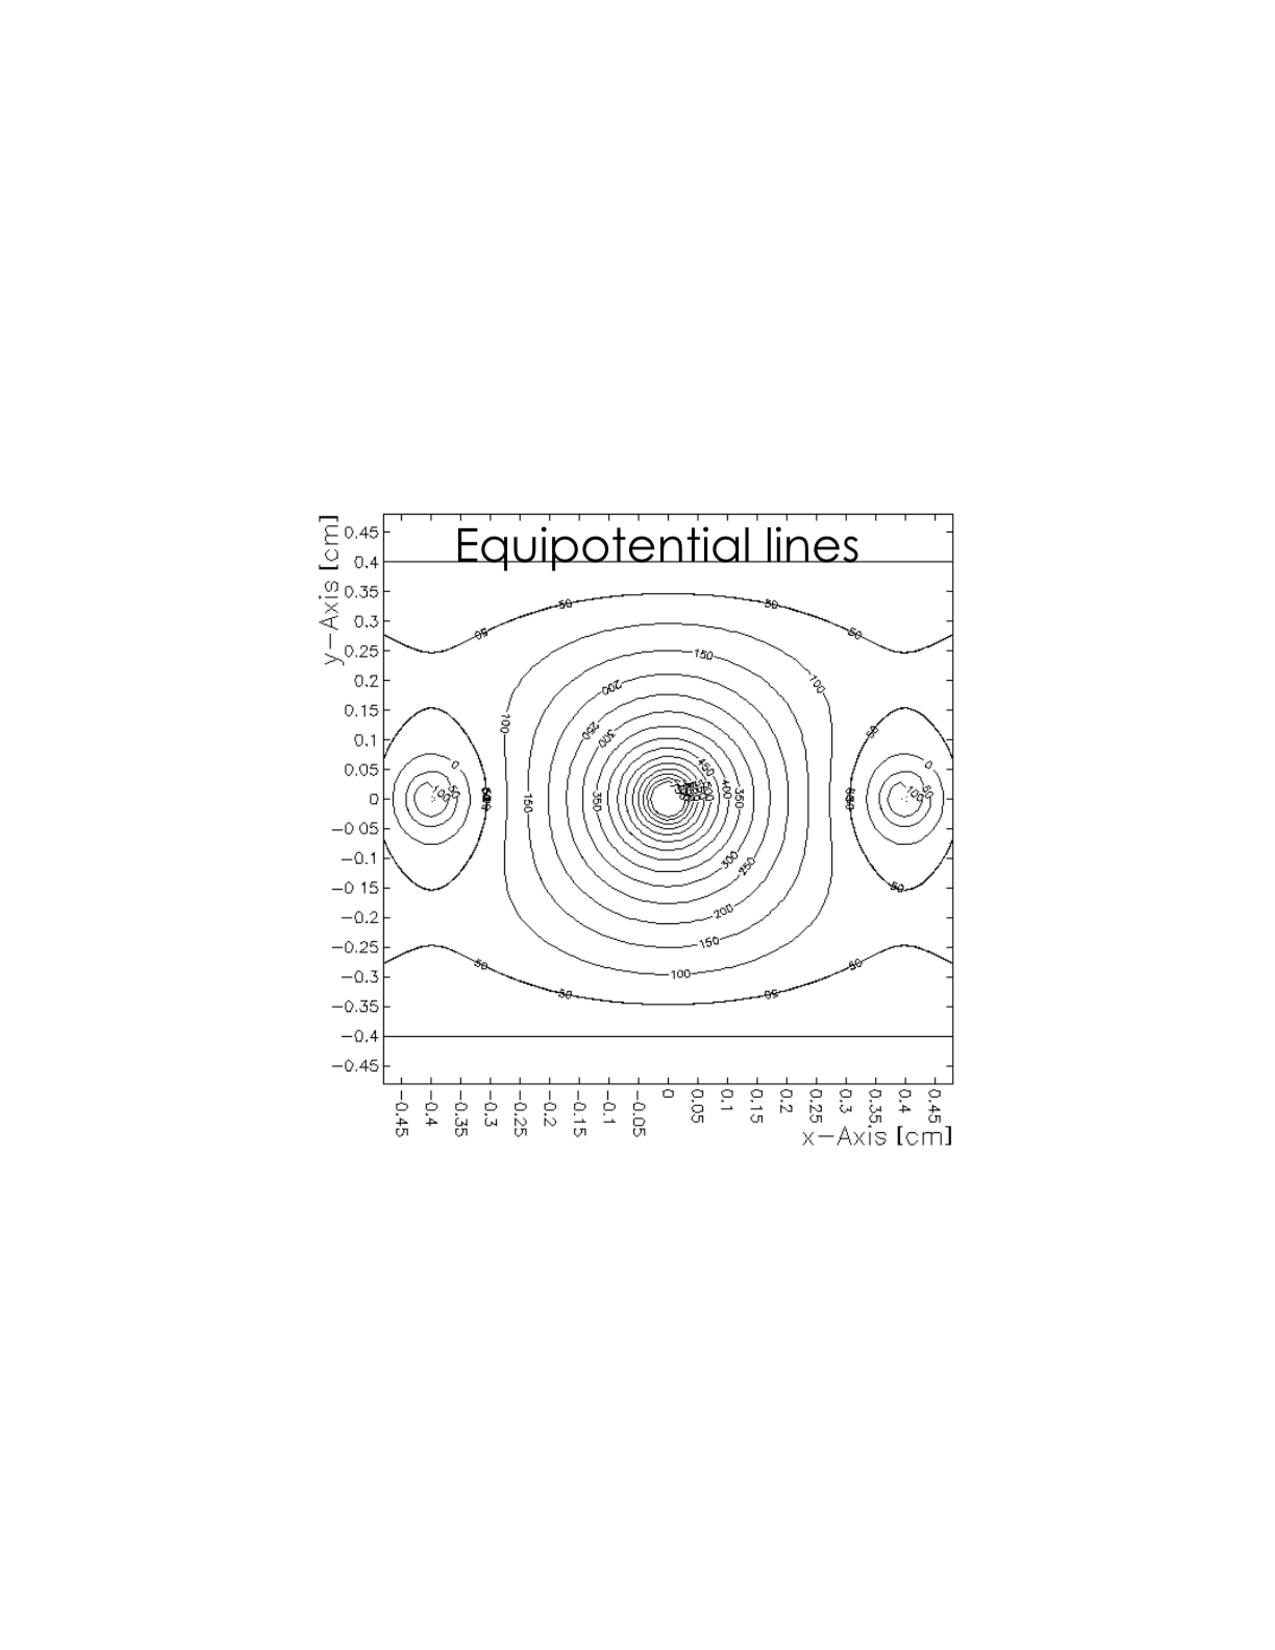
\includegraphics[width=0.6\textwidth, trim=4.5cm 8cm 4.5cm 8cm, clip]
                  {dcCellFieldLines}
  \caption{View down the axis of a drift cell and the equal voltages for this
    drift cell configuration.  This image is taken from~\cite{ran_bi}}
  \label{fig::dcCellFieldLines}
\end{figure}

Between the anodes and cathodes of a drift cell is a gas mixture.  The high
energy charged particles which enter the chamber ionize this gas mixture.  For
each track passing through the chamber, multiple primary ionization electrons
are produced and these electrons drift to the signal wire.  The number of
primary ionization electrons produced however, is not enough to create a
detectable signal on the sense wires.  For this reason the electric field
increases as the inverse of the distance from the sense wire which allows the
primary ionization electrons to gain enough energy to further ionize the gas and
ultimately produce an electron avalanche near the sense wire.  The signal
created from this electron avalanche is strong enough to detect.  A typical
detector is built so that an avalanche can occur before the sense wire but not
before a cathode wire.  This is accomplished by constructing the chamber with
sense wires having a much smaller diameter than the field wires, meaning the
electric field near the sense wire can be much larger than the electric field
near the field wire.

An important factor for a drift chamber is that the location of the primary
ionized electrons can be determined within a drift cell.  This knowledge allows
for a better position determination of the passing track as compared to a
multi-wire proportional chamber.  Each sense wire records the time a signal was
detected from a track.  For the same track, the trigger records the time the
track enter the drift chamber and therefore the difference in time between the
sense wire time and the trigger time is the drift time.  For a drift chamber it
is possible to produce a calibration curve which determines the position within
a drift cell for a given drift time.  This calibration curve is so-called the RT
relation.

Even with a properly calibrated RT relation the track location is ambiguous from
only one drift cell.  This is because a single drift cell can only determine a
track location as a distance from the sense wire.  Therefore it is ambiguous
where along the sense wire the track passed and also if the track passed to the
left or right of the sense wire.  For this reason drift chambers are built with
several planes in series.  A drift cell with the same orientation but shifted
with respect to the first drift cell is used to distinguish left and right
ambiguity and another cell with an orientation at an angle with respect to the
first is used to determined where along the wire the track passed.


\section{Preparation for DC05}

One of the first steps in preparation for constructing DC05 was to simulate the
detector response using Garfield~\cite{garfield}.  The purpose of these
simulations was to determine an operating threshold capable of achieving a
200~$\mu$m position resolution.  With this position resolution goal in mind,
Garfield simulated the electric potential field in each drift cell, as shown in
Fig.~\ref{fig::dcCellFieldLines}, and was able to determine the arrival times
for ionized electrons as a function of the number of primary ionized electrons
for detection.  This is important because the timing distribution for electron
arrival times gets wider and therefore worsens the position knowledge as the
number of primary electrons required for a signal increases.  The variance of
the electron arrival times was then used to determine the position resolution as
a function of the number of primary electrons needed for detection.  As is shown
in Fig~\ref{fig::PosResVnumElec}, the threshold should be tuned to detect the
amplification of the fifth primary electron~\cite{ran_bi}.  As is shown in
Fig.~\ref{fig::currentVtimeFifthElec} based on the simulation of the integrated
induced current versus the drift arrival time, the threshold for detecting the
signal should be no greater than 4~fC~\cite{ran_bi}.  This threshold charge is
determined by multiplying the induced current by the arrival time.  The
threshold was accordingly one of the design goals for the front-end electronics.

\begin{figure}[h!t]
  \centering
  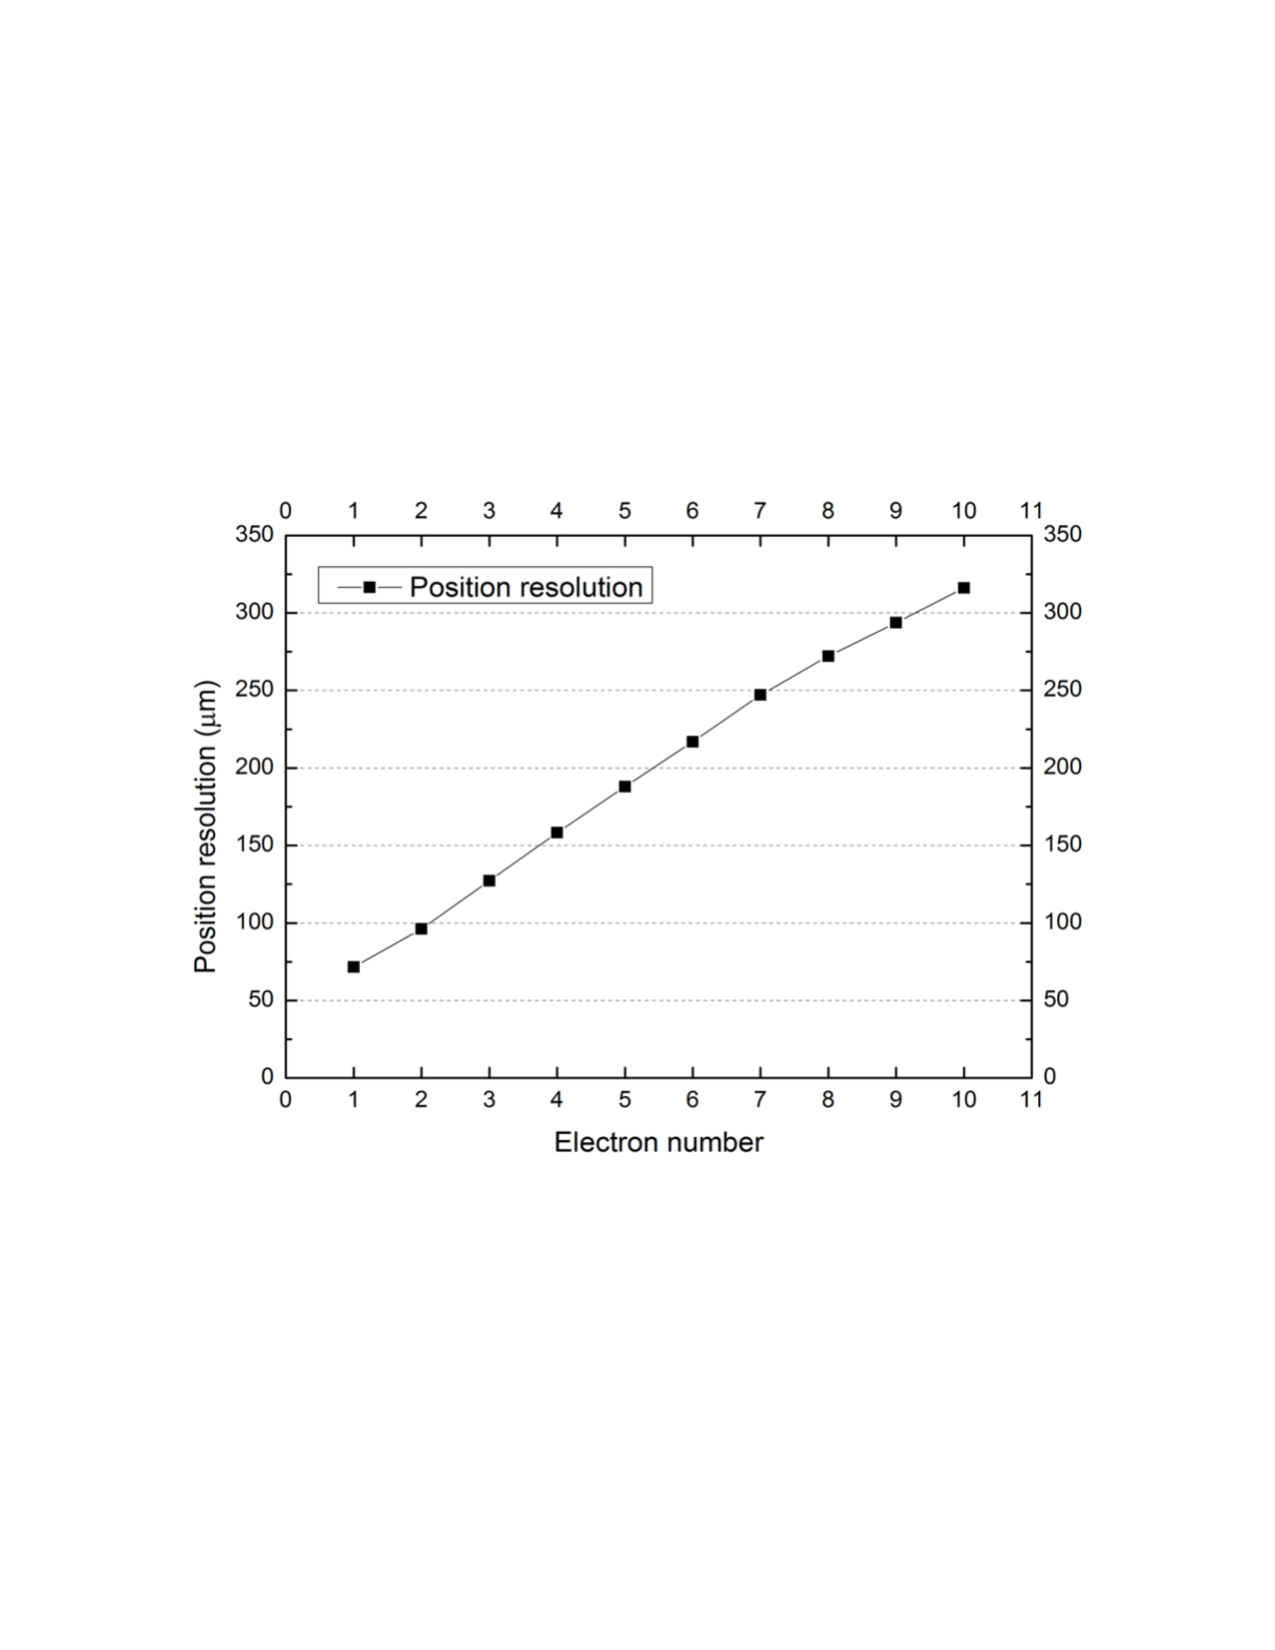
\includegraphics[width=0.55\textwidth, trim=3cm 8cm 3cm 8cm, clip]
                  {PosResVnumElec}
  \caption{A simulation of the position resolution as a function of the number
    of primary electrons needed to record a signal.  This image is taken
    from~\cite{ran_bi}}
  \label{fig::PosResVnumElec}
\end{figure}

\begin{figure}[h!t]
  \centering
  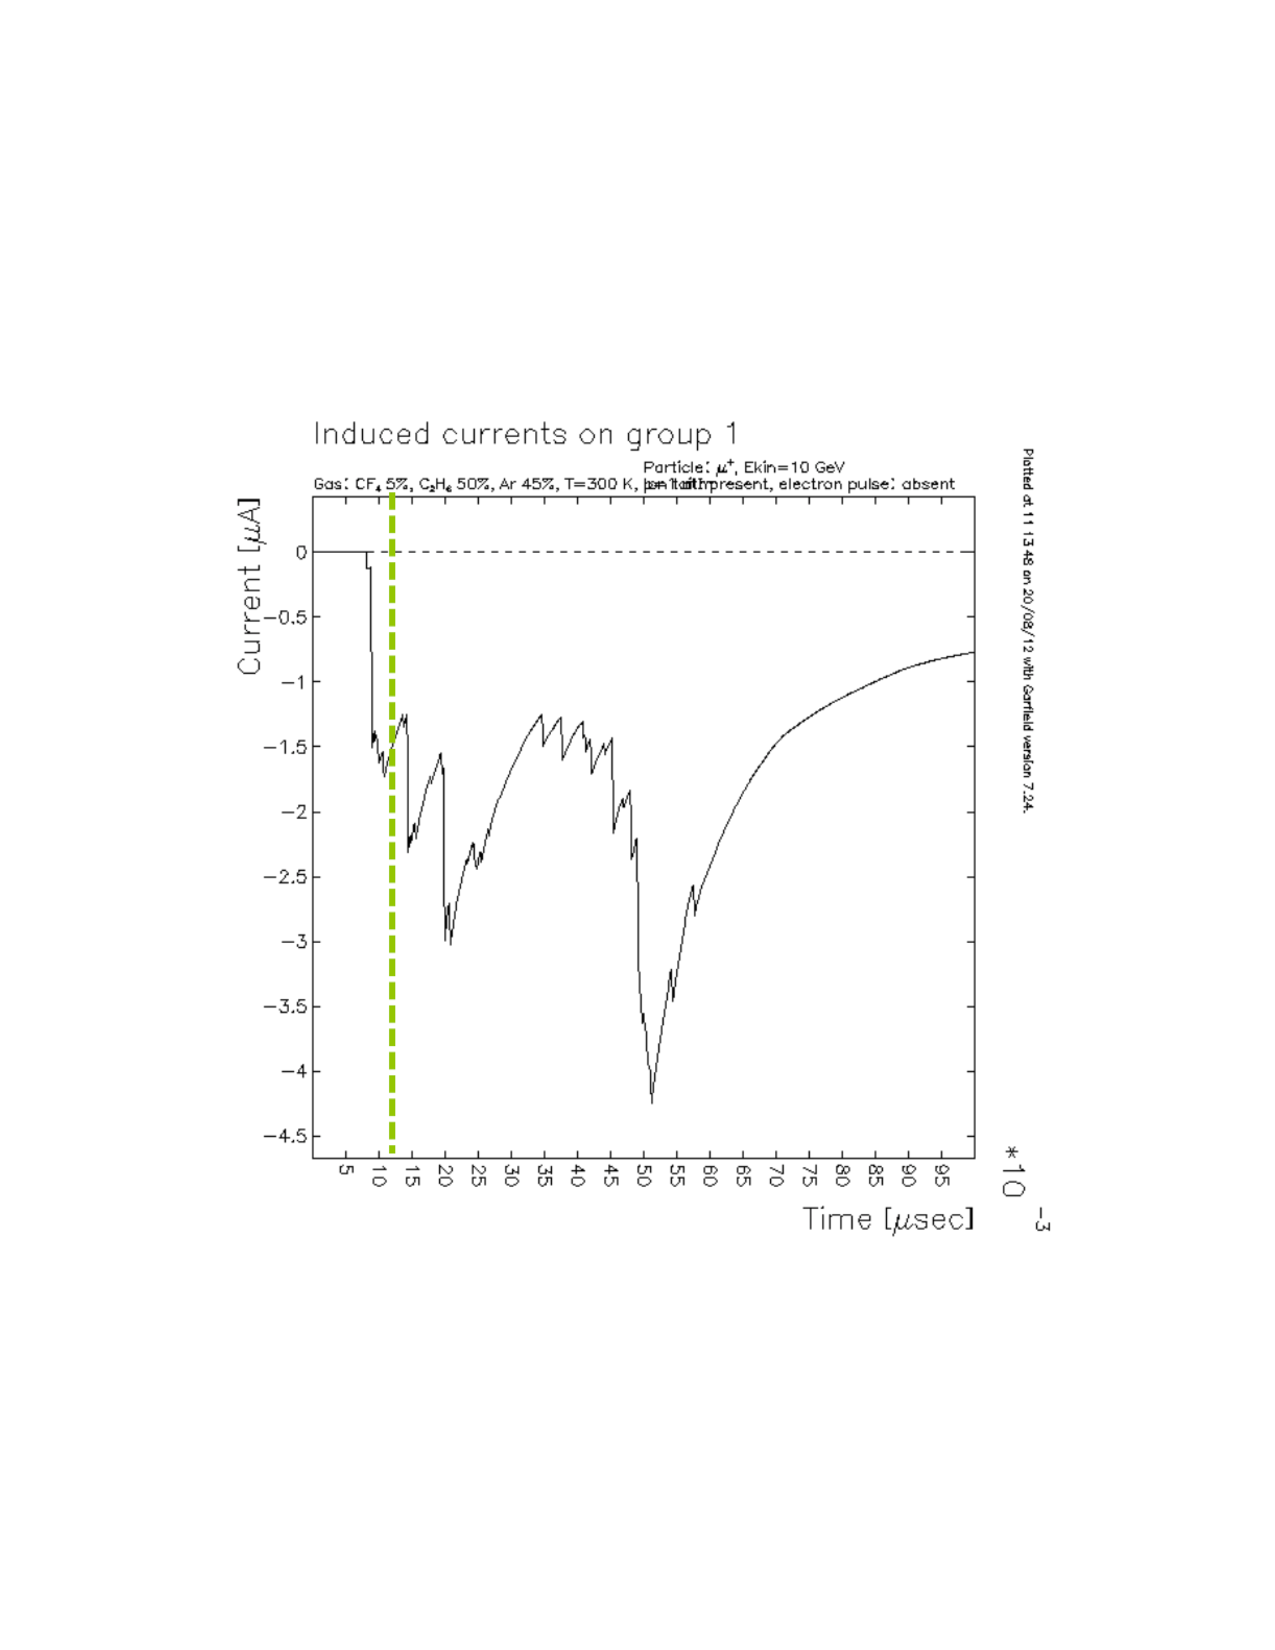
\includegraphics[width=0.55\textwidth, trim=3cm 6cm 3cm 6cm, clip]
                  {currentVtimeFifthElec}
  \caption{Garfield simulation of the induced signal current versus the arrival
    time.  The green line corresponds to the arrival time of the fifth election.
    This image is taken from~\cite{ran_bi}}
  \label{fig::currentVtimeFifthElec}
\end{figure}

Two prototypes were built to gain hands on building expertise in preparation for
construction.  Both of these prototypes were constructed in a clean room in the
Nuclear Physics Lab (NPL) at UIUC.  Much of DC05 was built at the NPL as well.
The two prototypes were called prototype A and prototype B.  Prototype A,
Fig.~\ref{fig::protoTypeA}, consisted of 1 plane, eight sense wires, 9 field
wires and was 50~cm in length.  Prototype B on the other hand consisted of two
planes with 16 sense wires per plane and a length of 163~cm.  Prototype A was
tested with beam at DESY and was shown to achieve 200~$\mu$m
resolution~\cite{choi}.  Both of these prototypes were built using similar
materials and construction techniques as the full size detector.  In particular
these two prototypes were the needed experience for working with sense wires
having a diameter of 20~$\mu$m.

\begin{figure}[h!t]
  \centering 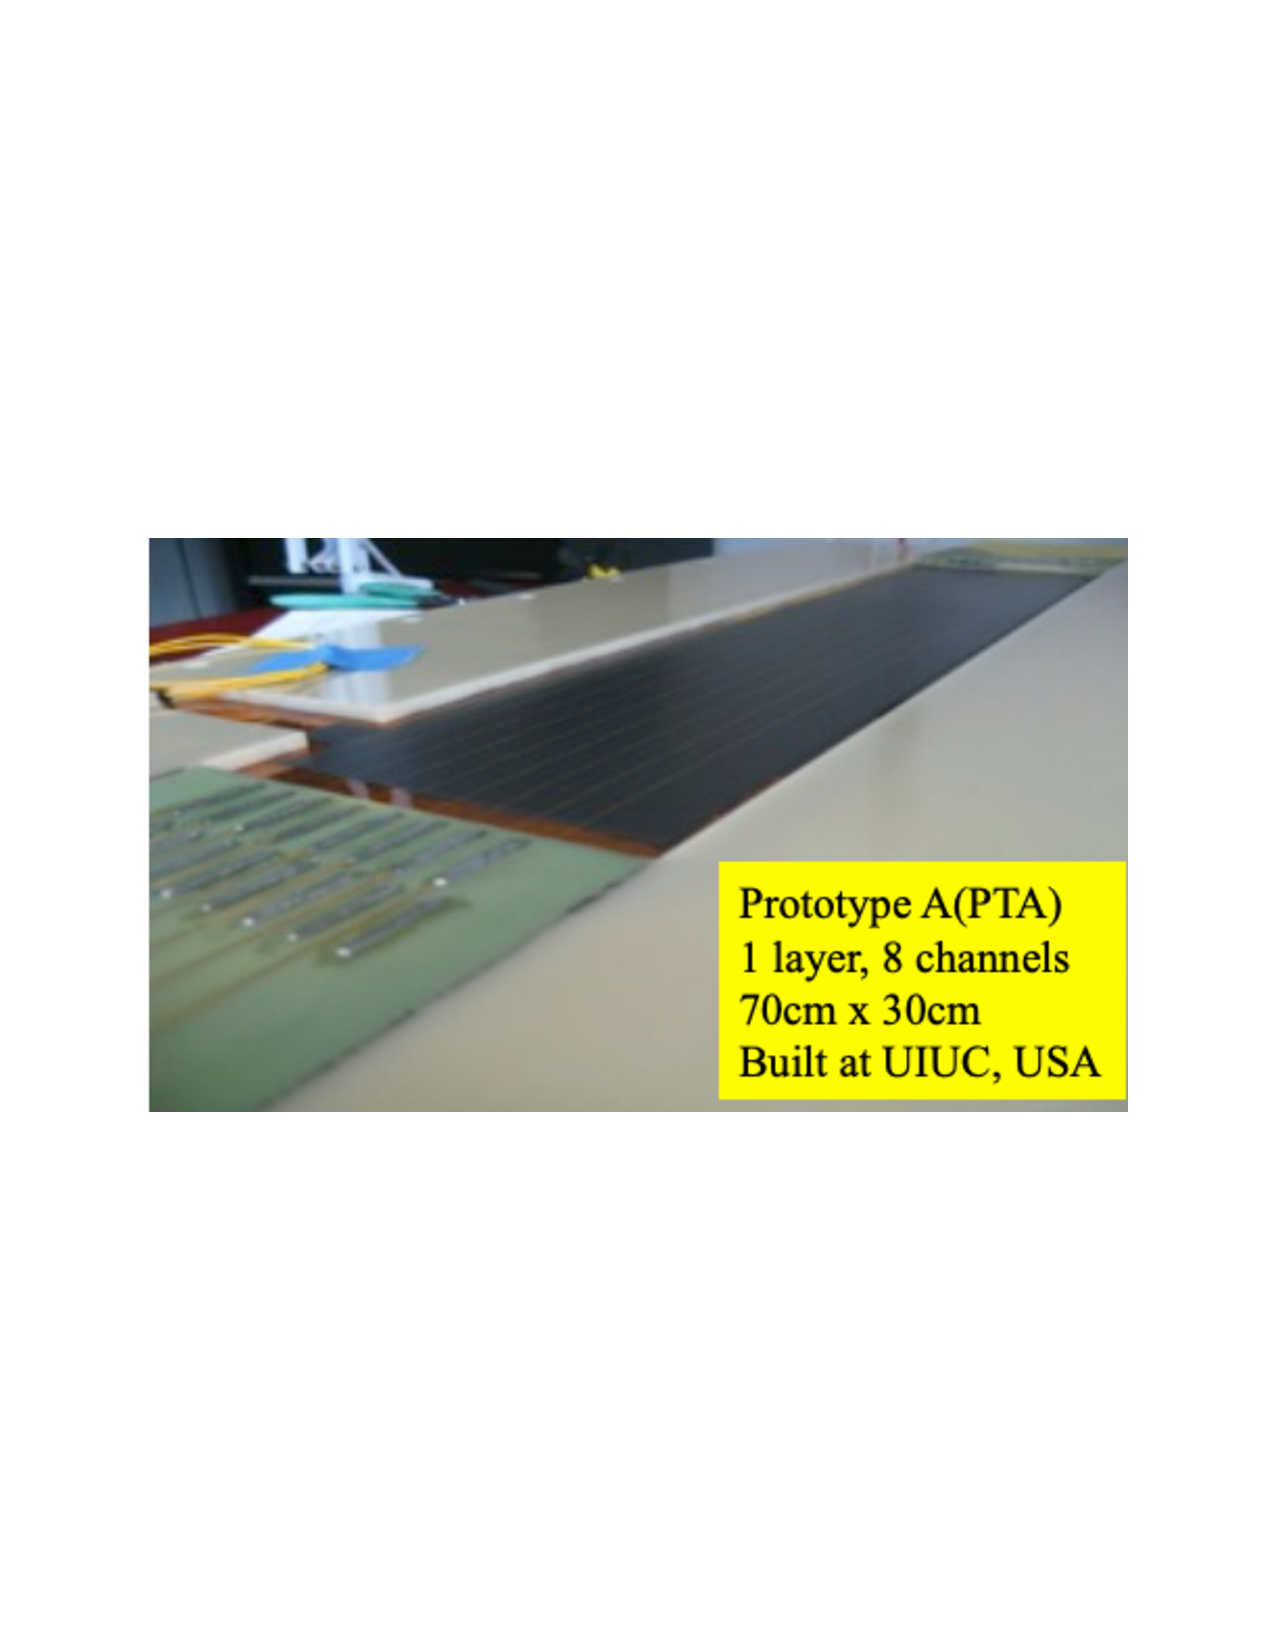
\includegraphics[width=0.6\textwidth, trim=2.5cm 8cm 2.5cm 8cm,
    clip]{protoTypeA}
  \caption{Inside view of prototype A.  This image was taken from~\cite{choi} }
  \label{fig::protoTypeA}
\end{figure}


\section{Design}

\begin{figure}
  \centering 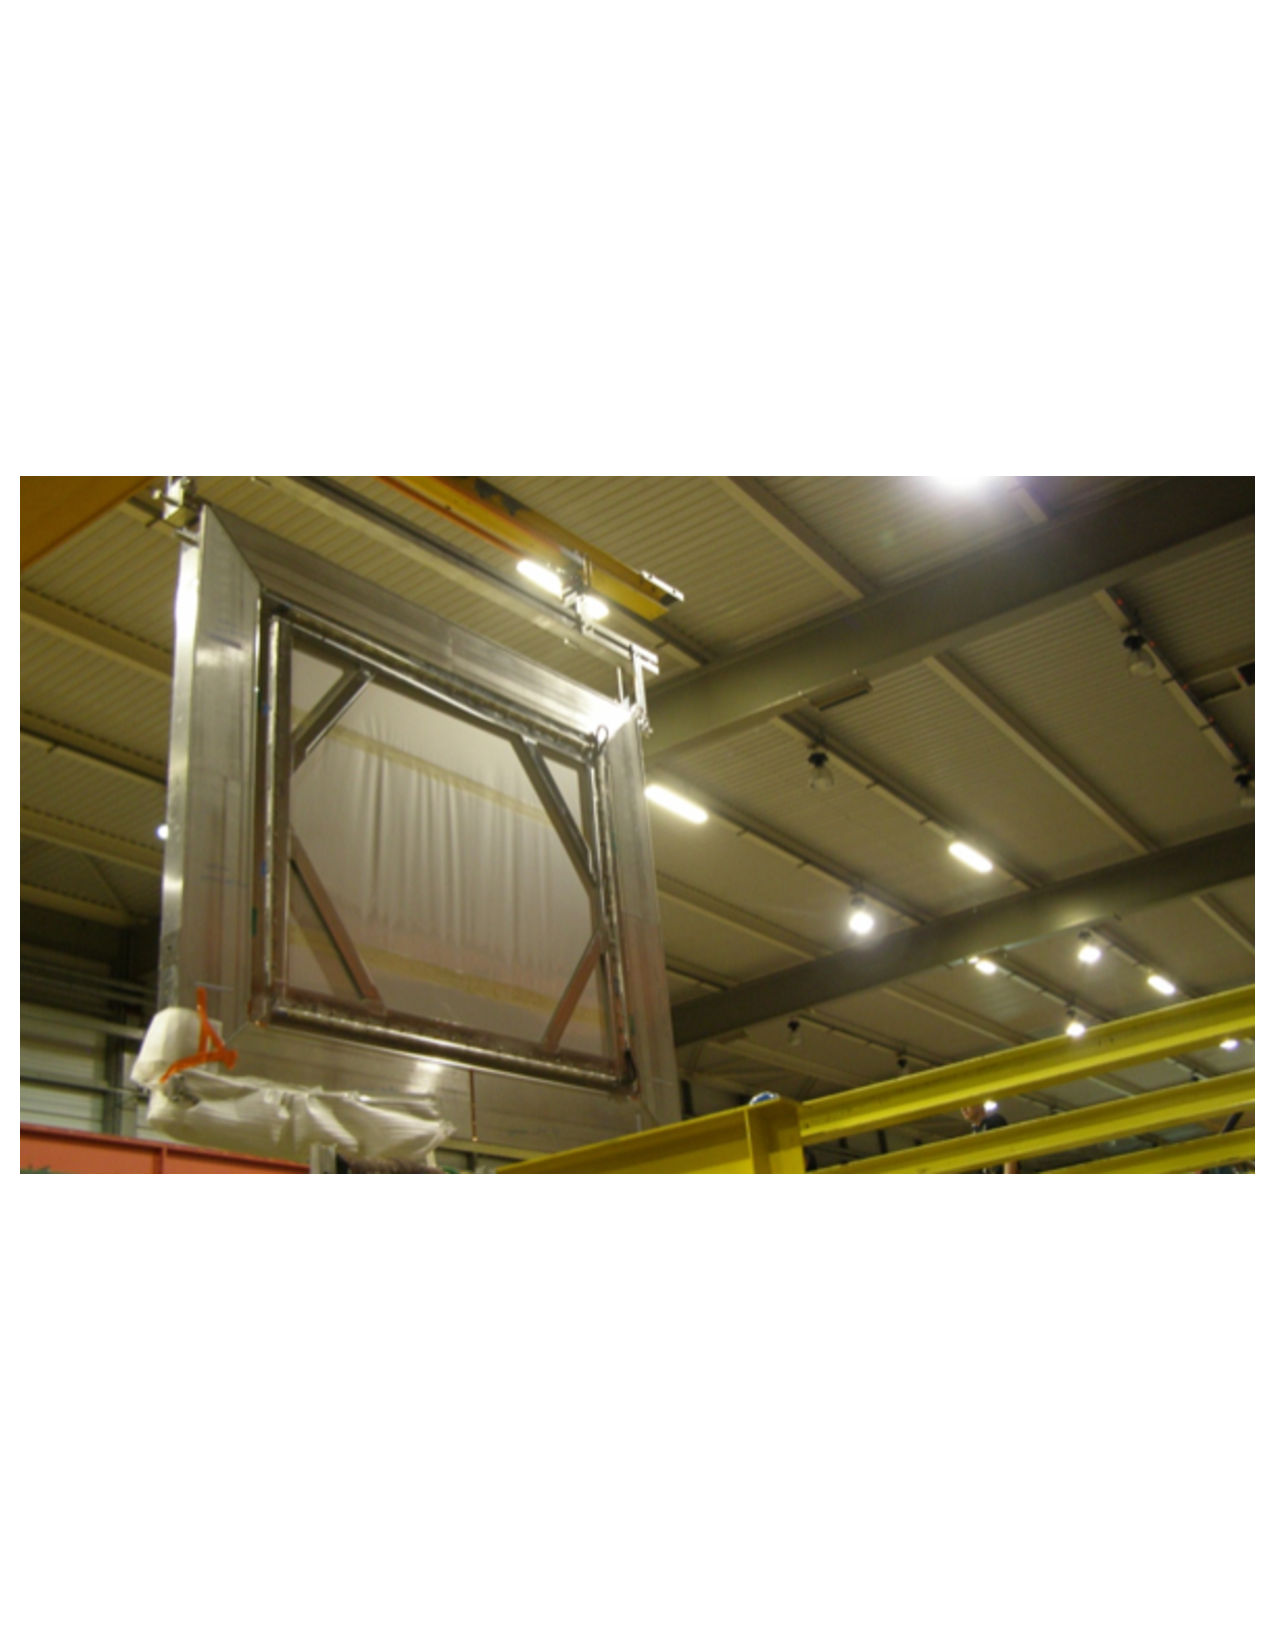
\includegraphics[width=0.7\textwidth, trim=2.5cm 8cm 2.5cm 8cm,
    clip]{DC05_full}
  \caption{}{The completed DC05 being craned into the COMPASS large area
    spectrometer.}
  \label{fig:DC05}%
\end{figure}

The design of DC05, figure~\ref{fig:DC05}, was based off a previous large-area
tracker at COMPASS.  DC05 has an active area of 249x209cm$^2$ and consists of
eight detector planes.  The eight planes of DC05 correspond to four views, where
each view measures a coordinate.  The coordinates measured from DC05 are the
horizontal, vertical and $\pm$ 10$^{\circ}$ with respect to the horizontal.  The
horizontal and vertical coordinates consist of 2x256 sense wires and the offset
to horizontal coordinates each consist of 2x320 wires for increased acceptance.
In total DC05 includes 2304 sense wires and 2312 field wires.  Each plane was
made from a G-10 frame and five frames stacked together constituting a view.
The whole detector was closed in with two precision, stainless steel stiffening
frames, which were assembled with aluminized mylar as a gas window.

The views of DC05 consist of three cathode layers and two anode layers.  The
cathodes layers were made from carbon paint sprayed on a 25~$\mu$m thin mylar
layer.  There were two single-layer cathodes layers and one layer with carbon on
two sides within each view.  Fig.~\ref{fig::DC05_layers} shows a side view of
the layers of DC05.  Additionally a 30~cm circular so-called beam killer was
added to the cathodes to control the efficiency in the central part of the
detector.  The cathodes were nominally set to -1675~V and the beam killer
voltage was set to -900~V for zero efficiency in the high flux central region.
The voltage on the beam killer can however be raised above the amplification
threshold if the beam flux is reduced and it is desirable to study the central
region.

\begin{figure}[h!t]
  \centering 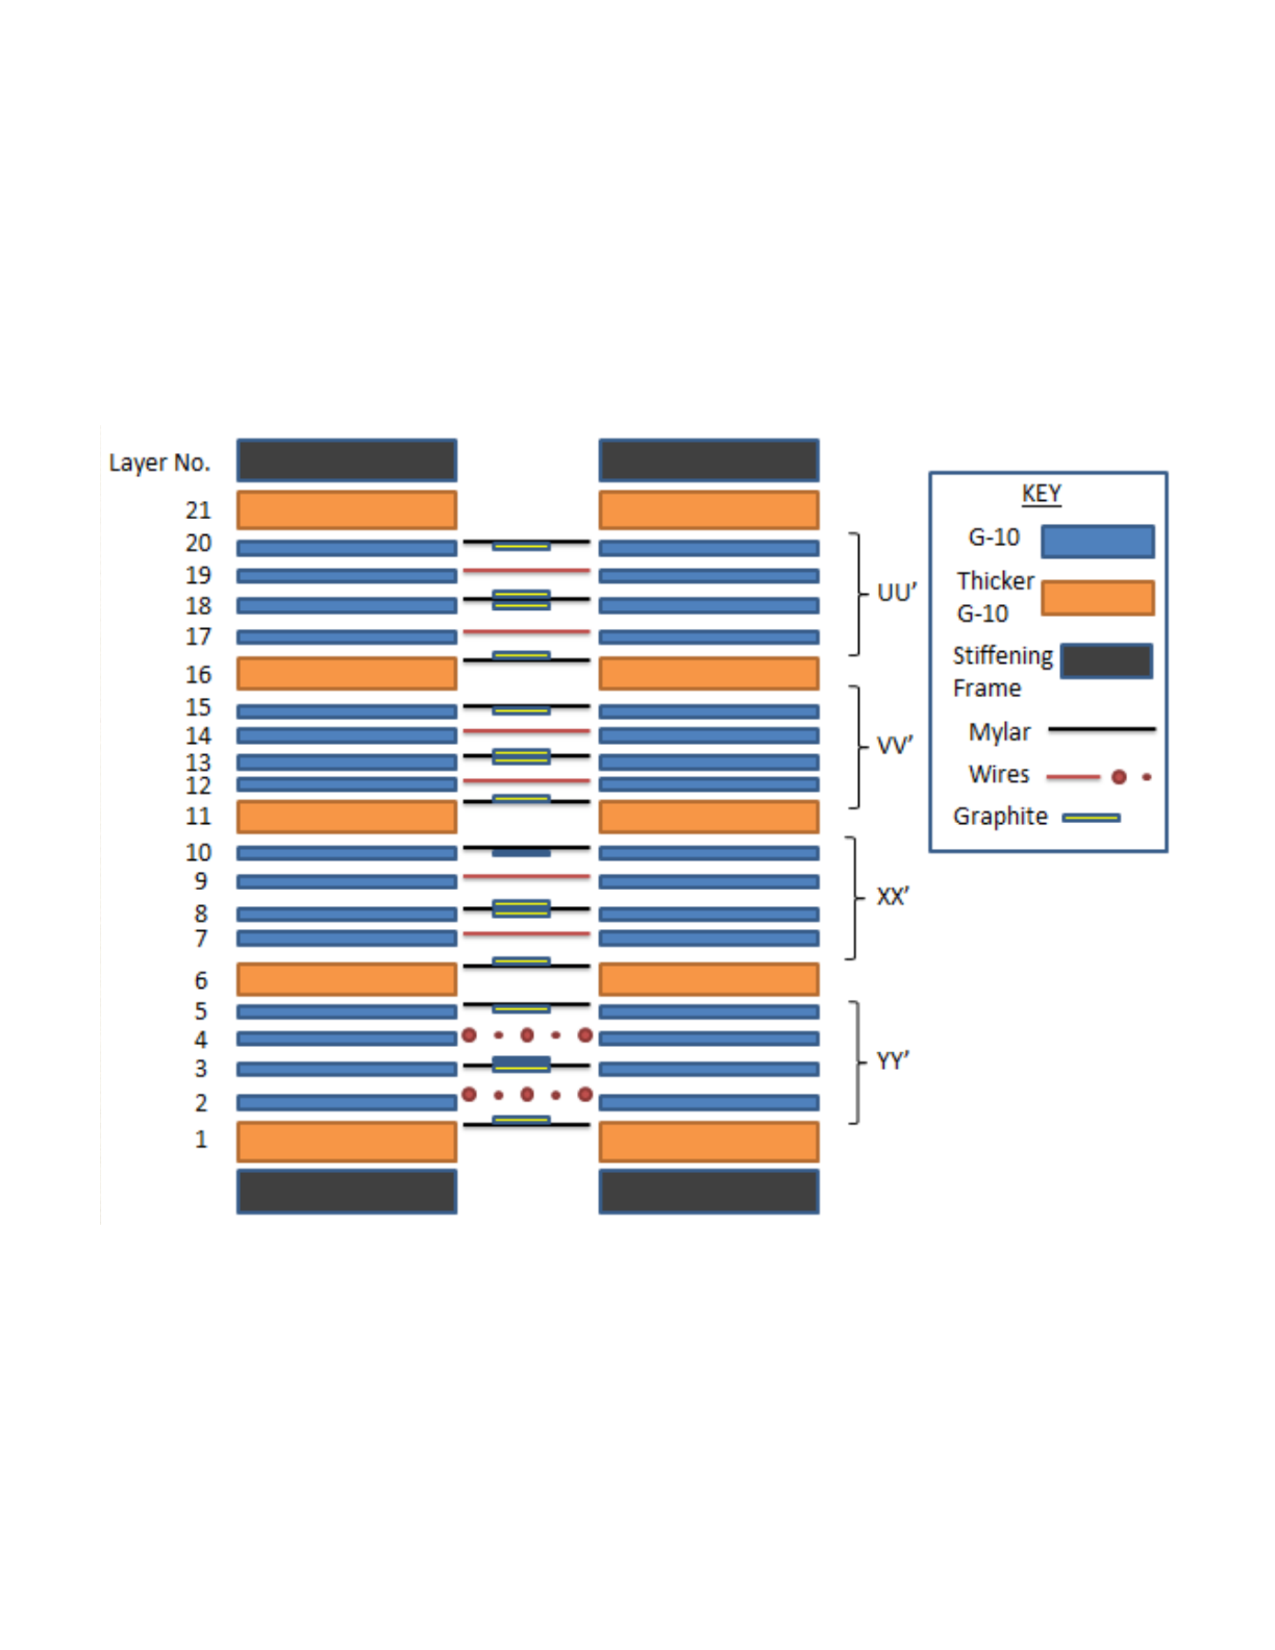
\includegraphics[width=0.7\textwidth, trim=0.2cm 7cm 0.2cm 2cm,
    clip]{DC05_layers}
  \caption{A side view sketch of the layers in DC05}
  \label{fig::DC05_layers}
\end{figure}

The anode layers were made from alternating 20~$\mu$m gold-plated tungsten sense
wires and 100~$\mu$m gold-plated copper beryllium field wires, as depicted in
figure~\ref{fig:driftcell}.  Gold plating was used for both sense and field
wires to prevent aging effects.  The field wires were also placed at -1675~V and
the sense wires were at 0~V.  The nominal gain of DC05 is approximately 10$^4$.

\begin{figure}
  \centering 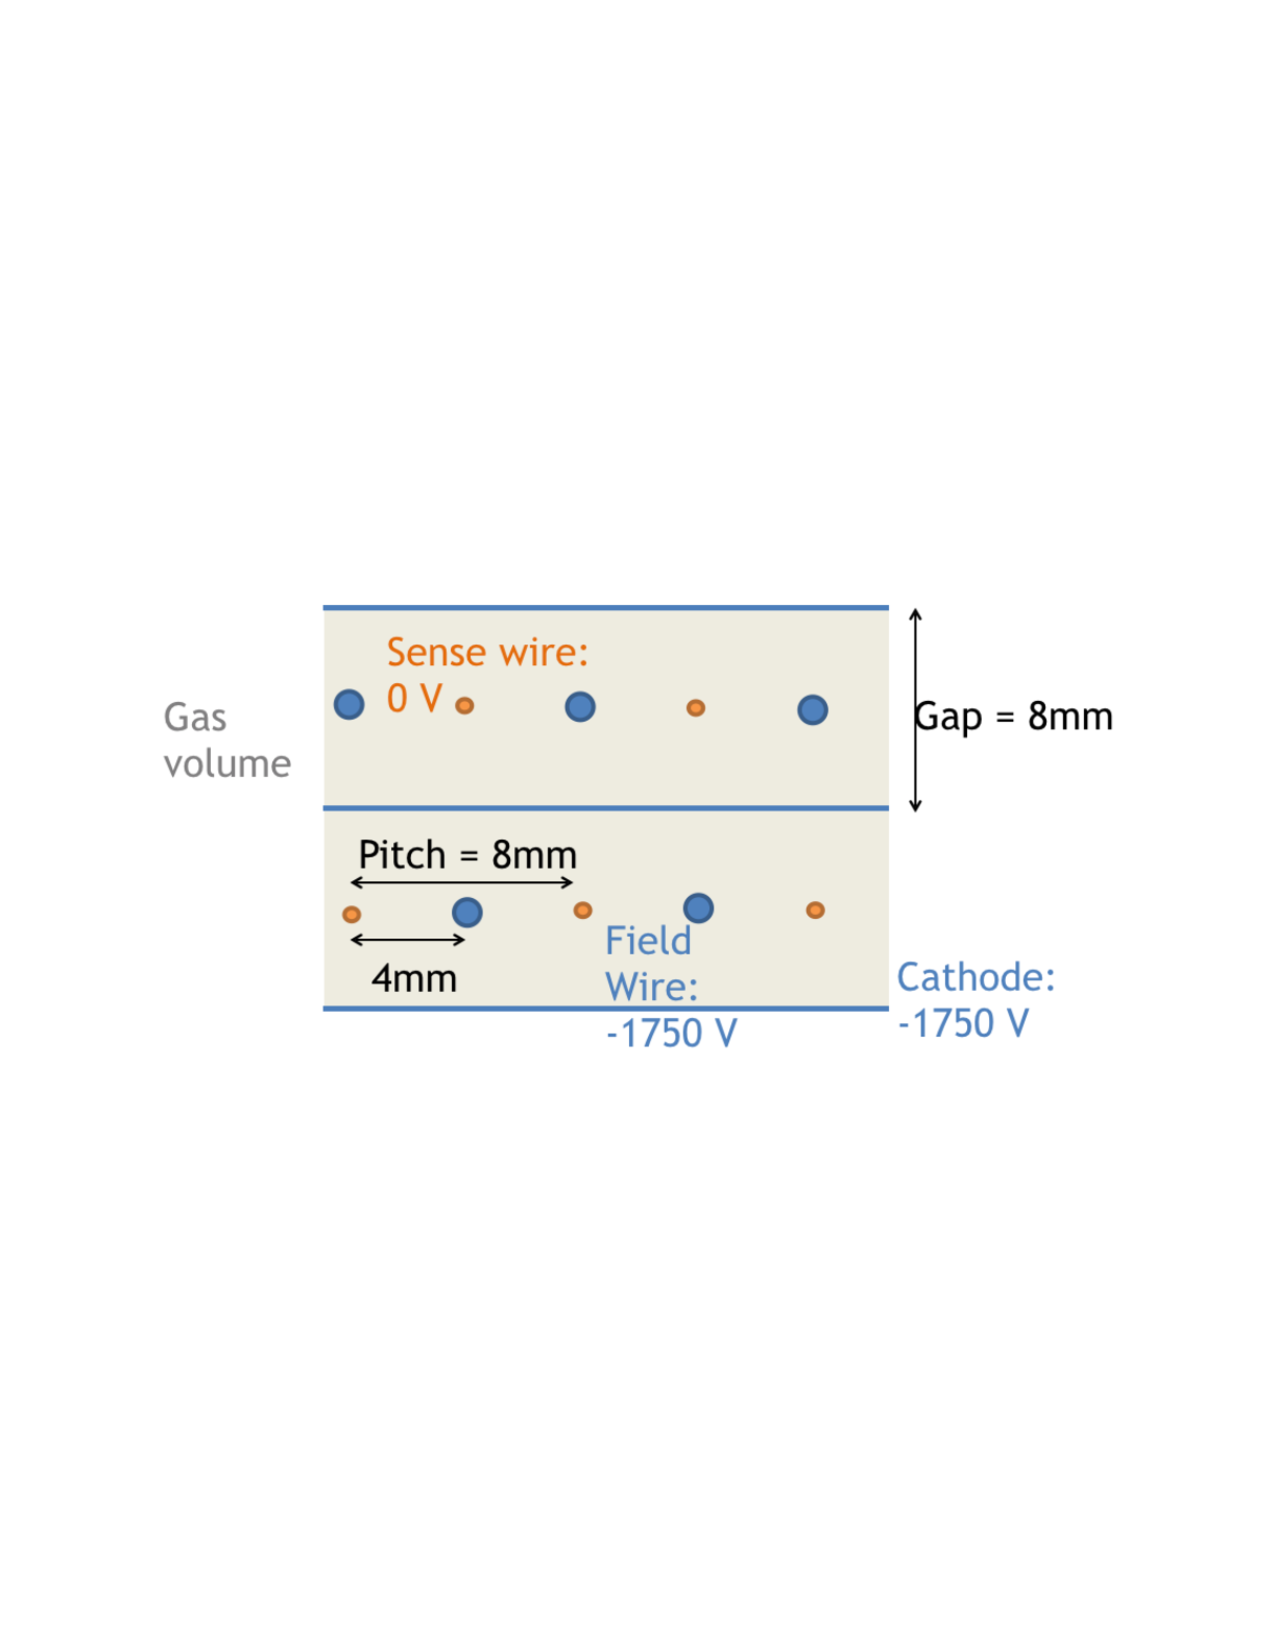
\includegraphics[width=0.5\textwidth, trim=2.5cm 10cm 3cm 10cm,
    clip]{DriftCell}
  \caption{}{The drift cell dimensions of one plane in DC05}
  \label{fig:driftcell}%
\end{figure}

During data taking, DC05 is filled with a mixture 45\% argon, 45\% ethane and
10\% Cf$_4$.  The noble gas, argon, is the gas that is ionized and amplified,
while ethane is used as a quencher and CF$_4$ is used to reduce aging effects.
The quencher, ethane, absorbs photons from the electron avalanche which could
pair produce and therefore make more electrons which would distort the electric
field in a drift cell.  The quencher therefore is used to reduce the avalanche
and ensure the drift cell electric field lines are closer to their design values.  


\section{Construction}

The construction of DC05 was carried out as precisely as possible starting with
the precision from the stainless steel stiffening frames.  The stiffening frames
where cut with the highest relative accuracy by cutting the two frames on top of
each other to a precision of 50~$\mu$m everywhere in their plane.  The precision
from the stiffening frames was transferred to the anode and cathode frames
through 40 positioning pins.  The G-10 frames were milled from strips at the NPL
using a precision milling machine.  Each four strips were then epoxied together
on top of one of the stiffening frames.

The cathodes had mylar stretched and epoxied to them using a custom built
stretching machine at CERN.  Fig.~\ref{fig::mylarStretching} shows the process
of stretching mylar on a cathode.  An external company then spray painted carbon
on them which was then polished till the resistance was approximately
30~k$\Omega /m$.  All the sense and field wires were hand soldered as shown in
Fig.~\ref{fig::wireSoldering}, and sequentially verified for position using a
microscope.  It was estimated the position placement of each sense wire was at
least as good as half the diameter of a sense wire or precise to 10~$\mu$m.

\begin{figure}[h!t]
  \centering 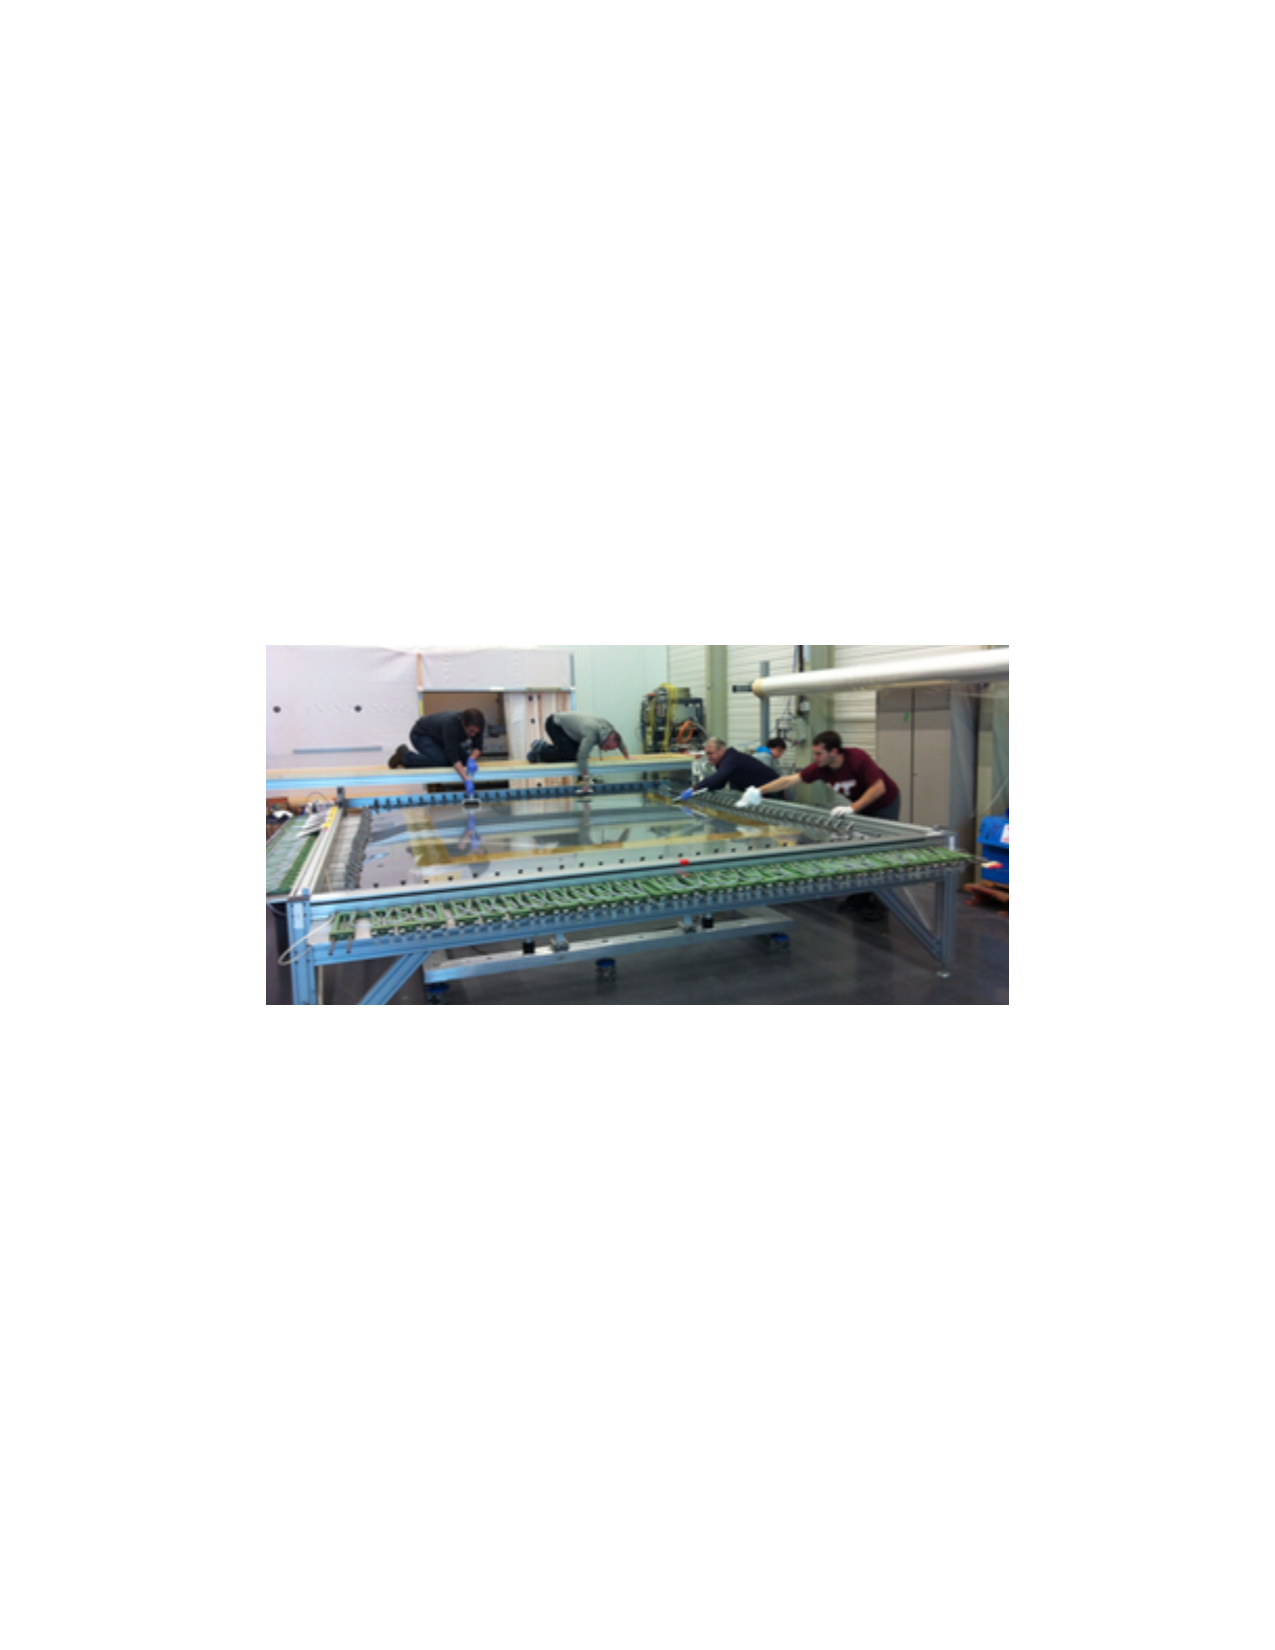
\includegraphics[width=0.6\textwidth, trim=5cm 12cm 5cm 10cm,
    clip]{mylarStretching}
  \caption{Stretching mylar on a cathode plane at CERN}
  \label{fig::mylarStretching}
\end{figure}

\begin{figure}[h!t]
  \centering \includegraphics[width=0.6\textwidth, trim=5cm 10cm 5cm 10cm,
    clip]{wireSoldering}
  \caption{Hand soldering DC05 wires in the clean room at the NPL}
  \label{fig::wireSoldering}
\end{figure}

The final assemble was done at CERN.  This consisted of stacking each of the 21
G-10 frames on top of the stiffening frame, Fig.~\ref{fig::cernFinalAssembly},
and attaching copper electronic shielding all along the exterior of the detector
to reduce electronic noise.

\begin{figure}[h!t]
  \centering \includegraphics[width=0.6\textwidth, trim=5cm 10cm 5cm 10cm,
    clip]{cernFinalAssembly}
  \caption{The process of stacking the G-10 frames at CERN}
  \label{fig::cernFinalAssembly}
\end{figure}

There were various tests performed throughout the construction process for
quality assurance before the final installation.  The starting tests were
measuring thickness and position of important cuts on the G-10 strips using a
micrometer.  G-10 strip thicknesses were iteratively milled until they reached
better than 50~$\mu$m in thickness accuracy.  The thickness deviation of the
whole detector including the stainless steel stiffening frames was better than
750~$\mu$m.  The mechanical tension of the sense wires was tested for stability
by ensuring the voltage difference between sense and field wires could reach as
high as 2400~V in air.  In addition the wire tension was cross-checked by
determining the resonance frequency with which the wires vibrated.  The
resonance frequency was determined by placing the wires in a constant magnetic
field and varying a sinusoidal current across each wire till the wires vibrated
maximally.  The leakage current between sense and field wires was verified to be
less than 100~nA at nominal voltage in air.  Finally amplification tests were
first performed using a strontium-90 source and verifying the counts per
electronics board increased below the radioactive source.


\section{2015 Performance}

The overall performance of DC05 was checked using the COMPASS reconstruction
software CORAL.  In all cases the view of study was excluded from the
reconstruction algorithm and the individual hit information for the view of
interest was saved to get an unbiased measurement.  The performance of DC05 is
determined by judging its response to real tracks.  In other words tracks that
are not falsely reconstructed, so-called ghost tracks.  To ensure these real
tracks with higher quality for performance evaluation, only tracks with a
primary vertex near the polarized target are considered.

The efficiency was found to be between 85\% and 90\% depending on the plane.
The efficiency was determined by searching for a hit in the DC05 plane of
interest within a road of 1.2~mm from the reconstructed track location.  The
road distance was chosen to be approximately six resolution deviations which is
standard at COMPASS.  Fig.~\ref{fig::DC05Yeff} shows the efficiency of one plane
of DC05.  Using the so called RT relation, figure~\ref{fig:RT_DC05Y2}, the
location of a track within a drift cell can be most accurately determined.  This
RT relation is tuned as a calibration to minimize the track residuals.  The RT
relation also varies depending on the beam type, intensity and the trigger type.

\begin{figure}[h!t]
  \centering \includegraphics[width=0.6\textwidth, trim=2cm 9cm 2cm 7cm,
    clip]{DC05Yeff}
  \caption{}{Two dimensional efficiency on the DC05Y1 plane.  The center region
    with zero efficiency is a result of the beam killer.}
  \label{fig::DC05Yeff}%
\end{figure}

\begin{figure}[h!t]
  \centering \includegraphics[width=0.6\textwidth, trim=3cm 9cm 3cm 8cm,
    clip]{RT_DC05Y2}
  \caption{}{Time versus position relation, or RT relation, after calibrating.
    The red fit shows the calibration determined.}
  \label{fig:RT_DC05Y2}%
\end{figure}

The double layer residual was used to determine the position resolution.  The
double layer residual is the difference between the expected positions of the
two planes in a view.  The double residual is defined as

\begin{equation}
  \label{equ::doubleRes}
  \Delta \mathrm{u}_{\mathrm{double \; residual}} = (\mathrm{u}_{\mathrm{plane
      \; 1}} - \mathrm{u}_{\mathrm{track}}) - (\mathrm{u}_{\mathrm{plane \; 2}}
  - \mathrm{u}_{\mathrm{track}}) = \mathrm{u}_{\mathrm{plane \; 1}} -
  \mathrm{u}_{\mathrm{plane \; 2}},
\end{equation}
\noindent
where u$_{\mathrm{plane \; 1(2)}}$ is the hit position on plane 1(2) determined
from the detector of interested and u$_{\mathrm{track}}$ is the hit position
determined from reconstruction.  As can be seen in Eq.~\ref{equ::doubleRes}, the
double layer residual is independent of the track resolution and only depends on
the difference between detector hit positions.  As the detector was construction
with a known difference between these two cell hit positions, the double
residual distribution is expected to be a constant value.  Therefore the
variance of the double residual distribution is the addition of the variance of
the two individual planes.  That is

\begin{equation}
\sigma_{\mathrm{double \; residual}}^2 = \sigma_{\mathrm{plane \; 1}}^2 +
\sigma_{\mathrm{plane \; 2}}^2 = 2*\sigma_{\mathrm{plane \; 1}}^2,
\end{equation}

\noindent
where $\sigma_{\mathrm{plane \; 1(2}}$ is the position resolution of plane 1(2).
It is assumed that the position resolution is the same for each plane and
therefore

\begin{equation}
\sigma_{\mathrm{plane \; 1}} = \sigma_{\mathrm{plane \; 2}} =
\frac{\sigma_{\mathrm{double \; residual}}}{\sqrt{2}}
\end{equation}

\noindent
For the 2015 Drell-Yan physics taking the resolution achieved was
approximately 430~$\mu$m. This was determined by fitting the double residual
with a Gaussian to extract the variance and assuming equal variance per plane in
a view as is shown in Fig.~\ref{fig::DC05doubleRes}.

\begin{figure}[h!t]
  \centering \includegraphics[width=0.6\textwidth, trim=2cm 9cm 2cm 8cm,
    clip]{DC05doubleRes}
  \caption{The double residual distribution for the V plane together with a
    Gaussian fit in red to determine the variance of the distribution}
  \label{fig::DC05doubleRes}
\end{figure}

\chapter{Spectrometer Alignment} \label{ch::alignment}
\ifpdf
\graphicspath{{Chapters/Alignment/Figs/Raster/}{Chapters/Alignment/Figs/PDF/}{Chapters/Alignment/Figs/}}
\else \graphicspath{{Chapters/Alignment/Figs/Vector/}{Chapters/Alignment/Figs/}}
\fi

The alignment of the spectrometer is important for track reconstruction.
Alignment is a part of pre-processing which ensures all the tracking detectors
are centered relative to each other and therefore enables the track resolution
to be as accurate as possible.  Without accurate alignment, track reconstruction
is not possible and it is therefore not possible to analyze any data.  The
author of this thesis oversaw collection of alignment data and was
responsible for performing the alignment of the COMPASS spectrometer in 2015.

The objective of the alignment procedure is to produce a file called the
detectors.dat.  This file describes the parameters for all detectors at COMPASS
and in particular, gives their orientation in space.  For a tracking detector
plane, there are four parameters the alignment procedure updates: the x central
position, y central position, angle and the pitch.  The pitch refers to a sense
wire distance for wire chambers or central strip separation distance for
detectors with strip readouts.  One or two detectors.dat files was produced for
each data taking period, depending on how many alignment runs were recorded that
period.  The goal of the alignment procedure is to have all four parameters
aligned relative to a global reference frame in the COMPASS lab system.

The alignment procedure works by minimizing the distance between all the
detector plane hit positions and a track position.  The detector hit position is
the location the detector believes a particle passed through the plane and the
track position is the location the reconstruction believes the particle passed
through the detector plane.  The distance between this detector plane hit
position and the track position will from here on be referred to as the residual
distance.  One residual is determined per track per detector associated with the
track.  The task of simultaneously minimizing all the residuals is difficult
because there are over 300 detectors planes described in the detectors.dat.  To
accomplish this minimization, a large amount of quality data is needed and
several specific matrix manipulations are utilized in the minimization
procedure.  This chapters gives an overview of the alignment procedure and
includes some results from 2015.  For a more complete review see
reference~\cite{compassAlignmentNote}.


\section{Alignment Data}

The alignment data is produced from a dedicated low intensity muon beam.  The
intensity in 2015 was approximately 10$^5 \mu^-$/spill.  A muon beam is
desirable for alignment data because the beam muons interact less and therefore
allows the alignment procedure to assume straight tracks in the minimization
problem.  The lower intensity is chosen because this allows for the assumption
that only one track occurs per event and also the low intensity beam ensures a
reduction of detector pile up effects.  Reduction in pile up effects, makes
reconstruction in the central detector areas possible, and therefore the beam
killers on DC00, DC01, DC04 and DC05 can be set to an amplification voltage and
as well all the GEM detectors can have their central high voltages turned up to
an amplification voltage.

A dedicated trigger system is setup during alignment runs to maximize the
illumination of the tracking detectors.  The triggers used are a beam trigger,
veto trigger and a halo trigger.  While this trigger was good for illuminating
the detectors, there were some timing shifts relative to the normal Drell-Yan
trigger in 2015.  For this reason some of the drift chambers used a different
calibration curve shifted in time a few nanoseconds.

Two alignment runs of good quality are recorded either at the beginning, middle
or end of a data taking period.  The first alignment run is with the
spectrometer magnets off and the second is with the spectrometer magnets on.
The spectrometer magnets off run is used as a first iteration for the alignment
procedure to initialize the tracking detector positions.  The final alignment
positions are then determined from the spectrometer magnets on data.  

One physics run was also used to align detectors far from the beam line.
Particularly, the outer region of the straw detectors did not receive enough
statistics from the aligning runs.  Therefore the alignment of the outer straw
regions was performed with normal physics data.  The runs used for alignment
analysis in 2015 are listed in Table~\ref{tab::alignmentRuns}.

In 2015 the alignment runs were performed when the target solenoid was
polarizing the target.  The chicane magnets upstream of the target were
therefore turned off to ensure the beam momentum was traveling along the target
axis.  Normally to achieve the reduced intensity, the T6 target is switch to an
air target.  However in 2015, the T6 target head was not able to switch between
the different target lengths and therefore the maximum 500~mm target head was
always in use.  Therefore to achieve the desired lower intensity, a set of
collimeters upstream of the target reduced the aperture of the beam line till
the correct intensity was achieved.

\begin{table}[h!t]
  \centering
  \begin{tabular}{ |c|c|c|c|c|c| }
    \hline
    \textbf{Period}& \textbf{Sub-period}& \textbf{Magnets off run}&
    \textbf{Magnets on run}& \textbf{Physics run}&
    \textbf{detectors.dat name} \\ \hline
    
    W07& one \& two & 259360& 259361& 259363& detectors.259361.transv.dat
    \\ \hline

    W08& one \& two & 260072& 260073& 260100& detectors.260073.transv.dat
    \\ \hline

    \multirow{2}{2em}{W09}& one& 260625& 260626& 260661&
    detectors.260626.transv.dat \\
    & two& 260625& 260876& 261312&
    detectors.260876.transv.dat \\ \hline

    \multirow{2}{2em}{W10}& one& 261512& 261513& 261602&
    detectors.261513.transv.dat \\
    & two& 261512& 261513& 261974&
    detectors.261970.transv.dat \\ \hline

    W11& one \& two & 262423& 262425& 262612& detectors.262370.transv.dat
    \\ \hline

    W12& one \& two & 263139& 263140& 263175& detectors.263140.transv.dat
    \\ \hline

    W13& one \& two & 263636& 263637& 263851& detectors.263637.transv.dat
    \\ \hline

    W14& one \& two & none& 264428& 264429& detectors.264163.transv.dat
    \\ \hline

    W15& one \& two & 264614& 264722& 264736& detectors.264619.transv.dat
    \\ \hline
    
  \end{tabular}
  \caption{COMPASS 2015 alignment data runs}
  \label{tab::alignmentRuns}
\end{table}


\section{Procedure}

The starting point for alignment is a detectors.dat file with the tracking
detector positions determined from a survey.  The surveys are performed with the
spectrometer magnets off and the precision from a survey is around 1~mm.  Almost
all of the detectors at COMPASS have a position resolution better than the
survey precision however.  Furthermore, several detectors near SM1 can shift in
position due to the fringe field and therefore need a position determination
with the spectrometer magnets on.  For these reasons the alignment procedure is
needed to improve on the survey precision and achieve the best possible track
resolutions.

Between periods the starting detectors.dat file was the final detectors.dat from
the previous week.  Only for the first period were the survey positions used as
a starting position.  However, as long as the detector was not intentionally
moved, it is expected that the shifts in detector position only change due to
temperature effects and therefore do not change much.

\subsubsection{Alignment Parameters}

To best describe each detector relative to every other detector there are two
reference systems of interest.

The first reference system is the COMPASS main reference system labeled
\textit{Oxyz}.  This reference system can also be referred to as the COMPASS lab
system, where the z-axis is along the beam momentum direction, the y-axis points
vertically and the x-axis is such that the coordinate system is right handed.
The origin of this reference system is at the center of the target from the
original COMPASS setup.

The second reference system is the local reference system, which is labeled as
\textit{O'uvz}.  This reference system is different for each detector and has
its origin at the center of each detector center.  The z-axis coincides with the
z-axis in the COMPASS main reference system while the u-axis is in the direction
along the measured coordinate of the detector, and the v-axis is perpendicular to
the direction of the measured coordinate of this detector.  As an example, a drift
chamber with vertical wires measures a coordinate along the horizontal direction
and therefore it's u-axis is in the horizontal direction and it's v-axis is in
the vertical direction.  A drift chamber with horizontal wires, however,
measures a coordinate along the vertical direction and therefore it's u-axis is
in the vertical direction and it's v-axis is in the horizontal direction.

The alignment parameters are defined in \textit{O'uvz}.  The alignment procedure
updates the starting detectors.dat file by the shifts

\begin{align}
  \delta \mathrm{u} & \mathrm{: \; shift \; in \; u \; direction,}  \\
  \delta \theta & \mathrm{: \; shift \; in \; rotation \; angle,}  \\
  \delta \mathrm{z} & \mathrm{: \; shift \; in \; z \; direction,}  \\
  \delta \mathrm{p} & \mathrm{: \; shift \; in \; pitch.} 
\end{align}
\noindent
The shift in z direction has never converged however.  As a result the
z-coordinate from the survey is used as the final z position and the shift in
pitch is used as an effective shift in the z direction.

\subsubsection{Residual Function}

The goal of the alignment procedure is to minimize the sum of all the residuals
from each track and each detector associated with the track.  Due to the fact
that the alignment tracks are assumed to be straight, each track can be defined
by four parameters.  The track parameters, {\atrack}, are

\begin{enumerate}[label=\roman*:]
\item (x$^0$, y$^0$) the x and y coordinates at the main reference origin
\item (t$_{\mathrm{x}}^0$, t$_{\mathrm{y}}^0$) the tangents of the track
  momentum in the x and y directions at the origin of the main reference system
\end{enumerate}
\noindent
where the track parameters are defined for each track.  The alignment parameters
, {\adet}, on the other hand are defined for each detector and are the same for
all tracks.  The alignment procedure minimizes the $\chi^2$ function

\begin{equation}
  \chi^2 =
  \sum_{i=1}^{i=n_{\mathrm{tracks}}}\sum_{j=1}^{j=n_{\mathrm{detectors}}}
  \frac{\mathrm{F}^2_{i,j}(\alpha_{\mathrm{T}, i}, \alpha_{\mathrm{D},
      j})}{\sigma_j^2},
  \label{equ::chi_align}%
\end{equation}
\noindent
where $\sigma^2_j$ is the position resolution of detector j, F$_{i,j}$ is the
residual distance of each detector j for each track i it is associated with.

The residual distance, F, depends on the track parameters and the detector
parameters.  For magnets off data the tracks are not bent at all and are
therefore straight tracks through out the whole spectrometer.  The x and y coordinates at position z are

\begin{align}
  \label{equ::trackPosOff}
  \mathrm{x} &= \mathrm{x}^0 +
  \mathrm{t}_{\mathrm{x}}^0(\mathrm{z}-\mathrm{z}^0), \\
  \mathrm{y} &=
  \mathrm{y}^0 + \mathrm{t}_{\mathrm{y}}^0(\mathrm{z}-\mathrm{z}^0),
\end{align}
\noindent
where z$^0$ refers to the position at the origin in \textit{Oxyz}.
Rotating these track positions from the main references system, \textit{Oxyz},
to the detector reference system, \textit{O'uvz}, the residual distance is

\begin{equation}
\mathrm{F} = \cos(\theta)[\mathrm{x}^0 +
  \mathrm{t}_{\mathrm{x}}^0(\mathrm{z}-\mathrm{z}^0)] +
\sin(\theta)[\mathrm{y}^0 + \mathrm{t}_{\mathrm{y}}^0(\mathrm{z}-\mathrm{z}^0)]
- \mathrm{u},
\end{equation}
\noindent
where u is the measured hit position from the detector at position z.  To show
the dependence on the alignment parameters

\begin{dmath} \label{equ::Falign}
  \mathrm{F}(\alpha_{\mathrm{T}}, \alpha_{\mathrm{D}}+\delta\alpha_{\mathrm{D}})
  = (1+\delta \mathrm{p})
  \Big \{ \cos(\theta + \delta \theta)
       [\mathrm{x}^0 + \mathrm{t}^0_{\mathrm{x}}(\mathrm{z}-\mathrm{z}^0)] +
       \sin(\theta + \delta \theta)[\mathrm{y}^0 + \mathrm{t}^0_{\mathrm{y}}
         (\mathrm{z}-\mathrm{z}^0)] \Big \} -
       (\mathrm{u} + \delta \mathrm{u}).
\end{dmath}
\noindent
In Eq.~\ref{equ::Falign}, the change in pitch would intuitively affect the u
position, however the change in pitch was moved to the track coordinates to make
derivatives of F independent of u.  This has no effect on the minimization of F.

In the case of magnets on data, the track positions need to have further
modifications from Eq.~\ref{equ::Falign}.  The magnetic field will bend the
tracks so the track positions determined in Eq.~\ref{equ::trackPosOff} need to
have further corrections.  The track positions with SM1 and SM2 on are
\begin{align}
  \label{equ::trackPosOn}
  \mathrm{x} &= \mathrm{x}^0 + \delta\mathrm{x} +
  (\mathrm{t}_{\mathrm{x}}^0 + \delta \mathrm{t}_{\mathrm{x}})
  (\mathrm{z}-\mathrm{z}^0), \\
  \mathrm{y} &= \mathrm{y}^0 + \delta\mathrm{y} +
  (\mathrm{t}_{\mathrm{y}}^0 + \delta \mathrm{t}_{\mathrm{y}})
  (\mathrm{z}-\mathrm{z}^0),
\end{align}
\noindent
where the $\delta_{\mathrm{x}}$, $\delta \mathrm{t}_{\mathrm{x}}$,
$\delta_{\mathrm{y}}$ and $\delta \mathrm{t}_{\mathrm{y}}$ changes are
determined from CORAL during the reconstruction process.  Even though the
spectrometer magnets have nominally vertical magnetic fields, there are still
fringe fields which are not vertical.  It is for this reason that CORAL also
calculates an updated track position in the y-coordinate.

The residual dependence on the alignment parameters defined for magnetic fields
on is then
\begin{dmath}
  \mathrm{F}(\alpha_{\mathrm{T}},
  \alpha_{\mathrm{D}}+\delta\alpha_{\mathrm{D}}) = 
  (1+\delta \mathrm{p})\Big \{
\cos(\theta + \delta \theta)[\mathrm{x}^0 + \delta\mathrm{x} +
  (\mathrm{t}^0_{\mathrm{x}}+\delta \mathrm{t}_{\mathrm{x}})
  (\mathrm{z}-\mathrm{z}^0)] +
\sin(\theta + \delta\theta)[\mathrm{y}^0 + \delta\mathrm{y} +
  (\mathrm{t}^0_{\mathrm{y}}+\delta \mathrm{t}_{\mathrm{y}})
  (\mathrm{z}-\mathrm{z}^0)]
\Big \}
- (\mathrm{u} + \delta \mathrm{u}).
\end{dmath}

\subsubsection{$\chi^2$ Minimization}
The $\chi^2$ function, Eq.~\ref{equ::chi_align}, is analytically minimized.
That is, the derivatives of Eq.~\ref{equ::chi_align} with respect to all the
track and alignment parameters are set to zero and these alignment parameters
are solved for.  This can be written

\begin{equation}
  \label{equ::chi2analytic}
  \frac{1}{2}\frac{\partial \chi ^2}{\partial \alpha_k} =
  \sum_{i}^{n_{\mathrm{tracks}}} \sum_j ^{n_{\mathrm{detectors}}}
  \frac{1}{\sigma_j^2}\frac{\partial \mathrm{F}_{i,j}}{\partial \alpha_k}
  \mathrm{F}_{i,j} = 0.
\end{equation}

\noindent
To perform this calculation the residual function is Taylor expanded in the
track and alignment parameters as
\begin{equation}
\mathrm{F} = \mathrm{F}^0 + \sum_k \frac{\partial \mathrm{F}}{\partial
  \alpha_k}\alpha_k.
\end{equation}

\noindent
Using this approximation for F, Eq.~\ref{equ::chi2analytic} can be written as a
matrix equation where the dimensions of the matrix are
(4n$_{\mathrm{detector}}$+4n$_{\mathrm{tracks}})\times$
(4n$_{\mathrm{detector}}$ +4n$_{\mathrm{tracks}})$.  This matrix form is written
as

\begin{dmath}
  \begin{bmatrix}
    \sum_i^{n_{\mathrm{tracks}}} \sum_j^{n_{\mathrm{detectors}}}
      \frac{1}{\sigma^2_j} \frac{\partial \mathrm{F}_{i,j}}{\partial
        \alpha_{\mathrm{D_1}}}\frac{\partial \mathrm{F}_{i,j}}{\partial
        \alpha_{\mathrm{D_1}}}
      & \dots &
      \sum_j^{n_{\mathrm{detectors}}}
      \frac{1}{\sigma^2_j}\frac{\partial \mathrm{F}_{i,j}}{\partial
        \alpha_{\mathrm{D_1}}}\frac{\partial \mathrm{F}_{i,j}}{\partial
        \alpha_{\mathrm{T_{4\mathrm{n}_{\mathrm{tracks}}}}}} \\
      \vdots & \ddots & \vdots \\
      \sum_j^{n_{\mathrm{detectors}}}
      \frac{1}{\sigma^2_j}\frac{\partial \mathrm{F}_{i,j}}{\partial
        \alpha_{\mathrm{T_{4\mathrm{n}_{\mathrm{tracks}}}}}}\frac{\partial
        \mathrm{F}_{i,j}}{\partial \alpha_{\mathrm{D_1}}} & \dots &
      \sum_j^{n_{\mathrm{detectors}}} \frac{1}{\sigma^2_j}\frac{\partial
        \mathrm{F}_{i,j}}{\partial
        \alpha_{\mathrm{T_{4\mathrm{n}_{\mathrm{tracks}}}}}}\frac{\partial
        \mathrm{F}_{i,j}}{\partial
        \alpha_{\mathrm{T_{4\mathrm{n}_{\mathrm{tracks}}}}}}
  \end{bmatrix}
  \begin{bmatrix}
    \alpha_{\mathrm{D_1}} \\
    \vdots \\
    \alpha_{\mathrm{T_{4\mathrm{n}_{\mathrm{tracks}}}}}
  \end{bmatrix}
  = -
  \begin{bmatrix}
    \sum_i^{n_{\mathrm{tracks}}} \sum_j^{n_{\mathrm{detectors}}}
      \frac{1}{\sigma^2_j}\frac{\partial \mathrm{F}_{i,j}}{\partial
        \alpha_{\mathrm{D_1}}} \mathrm{F}_{i,j}^0 \\
      \vdots \\
      \sum_j^{n_{\mathrm{detectors}}}
    \frac{1}{\sigma^2_j}\frac{\partial \mathrm{F}_{i,j}}{\partial
      \alpha_{\mathrm{T_{4\mathrm{n}_{\mathrm{tracks}}}}}} \mathrm{F}_{i,j}^0
  \end{bmatrix}.
  \label{equ::aliMatrix}
\end{dmath}    

\noindent
To solve Eq.~\ref{equ::aliMatrix}, the matrix on the left side must be inverted.
A normal alignment run however, results in over 200,000 tracks meaning this
matrix is huge and infeasible to invert.  Fortunately many of the entries in the
matrix are zero which allows that this matrix inversion can be reduced to
the inversion of several smaller matrices.

To perform the matrix inversion, note that Eq.~\ref{equ::aliMatrix} can be
written

\begin{equation}
  \label{equ::matrixToInvert}
  \begin{bmatrix}
    \sum_{i} \mathrm{C}_i & \vline \; \vline \; & \dots &
    \mathrm{G}_i & \dots \\
    \hline \hline
    \vdots & \vline \; \vline & \ddots & 0 & 0 \\
    \mathrm{G}^{\mathrm{T}} & \vline \; \vline & 0 \; & \Gamma_i & 0 \\
    \vdots & \vline \; \vline & 0 & 0 & \ddots
  \end{bmatrix}
  \begin{bmatrix}
    \alpha_{\alpha} \\ \hline \hline \vdots \\ \alpha_{\mathrm{T}_i}
    \\ \vdots
  \end{bmatrix}
  =
  \begin{bmatrix}
    \sum_i b_i \\ \hline \hline \vdots \\ \beta_i \\ \vdots
  \end{bmatrix},
\end{equation}

\noindent
where $\sum_i$C$_i$ and $\sum_i$b$_i$ include only derivatives of F$_{i,j}$ with
respect to alignment parameters, $\Gamma_i$ and $\beta_i$ include only
derivatives of F$_{i,j}$ with respect to track parameters and G$_i$ includes
derivatives of F$_{i,j}$ with respect to both alignment and track parameters.
Then reference~\cite{matrix_inv} shows that Eq.~\ref{equ::matrixToInvert} can be
inverted to give the alignment parameters as

\begin{equation}
\alpha_{\alpha} = \mathrm{C'}^{-1}\mathrm{b}',
\end{equation}
\noindent
where
\begin{equation}
\mathrm{C}' = \sum_i \mathrm{C}_i - \sum_i \mathrm{G}_i \Gamma_i^{-1}
\mathrm{G}_i^{\mathrm{T}},
\end{equation}
\noindent
and
\begin{equation}
\mathrm{b}' = \sum_i \mathrm{b}_i - \sum_i \mathrm{G}_i \Gamma_i^{-1}\beta_i.
\end{equation}


\section{Results}

The spectrometer alignment is performed in iterative steps.  In each iteration
of the alignment procedure, the matrix inversion, Eq~\ref{equ::matrixToInvert},
is performed and the alignment parameters are updated.  All alignment tracks
reconstructed in the first alignment iterations are based off of two pivot
detectors.  That is straight track parameters were determined from these two
pivot detectors and all detectors were aligned relative to these pivot
detectors.  In 2015 the pivot detectors were GM05 in LAS and GM08 in SAS.  After
each iteration the detector parameters are updated to reduce the overall
$\chi^2$ value.  Each new iteration is performed using the same data set and the
alignment parameters are better described with each iteration.

The procedure used in 2015 was as follows:
\begin{enumerate}
\item Align with magnets off data.  In this stage all the spectrometer detectors
  except the outer regions of the straw detectors are aligned.  This includes
  all the detectors downstream of the polarized target but does not include the
  beam telescope detectors.  Magnets off data is used as a first iteration and
  therefore only alignment in the u-coordinate is performed.
\item Align the same spectrometer detectors with magnets on data.  In these
  iterations the detectors are aligned for u-coordinate, angle and pitch.
\item Align the beam telescope detectors with magnets on data.  In these
  iterations the previous detectors are all used as pivots.  The beam telescope
  is therefore aligned relative to the spectrometer detectors.
\item Finally the outer region of the straws are aligned with physics data.  For
  this alignment, the spectrometer detectors are again used as the pivot.
\end{enumerate}

The quality of the alignment was monitored after each iteration and checked that
the procedure was converging.  In practice four iterations of each of the
previous steps were found to be sufficient for convergence.  To ensure the
alignment data was from quality tracks, only tracks with momentum reconstructed
and having reduced $\chi^2$ less than 30 were considered.

As all detectors but the pixal detector planes measure a coordinate in one
direction only, the detector positions are only updated in their measured
direction.  This can lead to detectors being well miss-aligned in the direction
orthogonal to their measured coordinate however.  To account for this, detector
planes were updated to match the u-position from a detector plane measuring a
different coordinate in the same detector station.  For example DC04X planes had
their y-coordinate determined from the DC04Y planes and DC04Y planes had their
x-coordinate determined from DC04X planes.

After each alignment iteration the quality of the alignment is accessed for each
individual detectors and for the spectrometer as a whole.  The quality
distributions to check after each iteration are described in the following list.

\begin{enumerate}[label=\roman*)]
\item The residual distribution, $\Delta$u, of each detector.  That is a
  distribution of
  \begin{equation}
    \Delta \mathrm{u} =
    \mathrm{u}_{\mathrm{track}} - \mathrm{u}_{\mathrm{detector}},
  \end{equation}
  where this distribution indicates if the detector is shifted along the
  direction of its measured coordinate.  This distribution is expected to be a
  Gaussian with a zero mean and an RMS value comparable to the position
  resolution of the detector.  Any deviation from a zero mean indicates the
  detector is shifted and a large RMS value indicates the detector is not
  performing as expected.  It the detector is not performing as expected the
  most obvious reason is the calibrations used for that detector are not
  accurate.  Fig.~\ref{fig::PositionResidual} shows an example of this
  distribution to monitor.
  \begin{figure}[h!t]
  \centering \includegraphics[width=0.5\textwidth, trim=4.5cm 9.5cm 4.5cm 9cm,
    clip]{PositionResidual}
  \caption{The residual distribution for a straw detector plane}
  \label{fig::PositionResidual}
  
\end{figure}
\item The change in the residual as a function of the detector's v-coordinate.
  In a wire detector for example, this is the change in the residual as a
  function of the distance along the wire.  This distribution,
  Fig.~\ref{fig::AngleResidual}, is expected to be uniformly zero.  A slope in
  this distribution indicates that the detector's angle is miss-aligned.
  \begin{figure}[h!t]
    \centering \includegraphics[width=0.5\textwidth, trim=4.5cm 9.5cm 4.5cm 9cm,
      clip]{AngleResidual}
    \caption{The residual as a function of the detector v-coordinate for a straw
      detector}
    \label{fig::AngleResidual}
  \end{figure}
  
\item The change in the residual as a function of the detector's u-coordinate.
  For a wire detector, this is the change in the residual as a function of the
  distance perpendicular to the wire.  This distribution,
  Fig.~\ref{fig::PitchResidual}, is also expected to be uniformly zero.  A slope
  in this distribution indicates that the detector is miss-aligned in it's
  z-coordinate or that its pitch is not described well.  Due to the fact that
  the alignment data is with straight tracks, the alignment in the z-coordinate
  has never been able to converge.  For this reason the pitch of the sensors on
  the detector is changed to account for this effective shift in z-position.
  The sensor pitch however, is never expected to be larger than the true
  detector pitch distance.  If the detector pitch is determined to be too large
  after the alignment, this indicates a problem.
  \begin{figure}[h!t]
    \centering \includegraphics[width=0.5\textwidth, trim=4.5cm 9.5cm 4.5cm 9cm,
      clip]{PitchResidual}
    \caption{The residual as a function of the detector u-coordinate for a straw
      detector}
    \label{fig::PitchResidual}
  \end{figure}

\item The reduced $\chi^2$, Fig.~\ref{fig::trackChi2ndf}, distribution of the
  reconstructed tracks.  With better alignment the track reduced $\chi^2$
  distribution will approach a theoretical distribution of a reduced $\chi^2$
  distribution.
  \begin{figure}[h!t]
    \centering \includegraphics[width=0.5\textwidth, trim=5cm 4.5cm 5cm 4.5cm,
      clip]{trackChi2ndf}
    \caption{The reduced $\chi^2$ from alignment data tracks}
    \label{fig::trackChi2ndf}
  \end{figure}
  
\item The global number of tracks reconstructed.  Better alignment
  implies that more detectors can be associated with a track and therefore more
  tracks will be reconstructed.
\end{enumerate}

\chapter{Analysis of High Mass Drell-Yan Transverse Spin Phenomena}
\label{ch::leftright}
\ifpdf
\graphicspath{{Chapters/HMAnalysis/Figs/}}
\fi

This chapter goes over the analysis techniques and results from the 2015
transversely polarized Drell-Yan data taking.  The chapter begins by describing
the data collection setup and the event selection criteria followed by the
analysis techniques used to determine asymmetry amplitudes.  The analysis
techniques described are: the standard transverse spin-dependent asymmetry (TSA)
analysis, Sec~\ref{sec::standTSA}, the double ratio analysis,
Sec~\ref{sec::doubleratio}, the $q_T$ weighted asymmetry analysis,
Sec~\ref{sec::qtweighted}, and finally the left-right asymmetry analysis,
Sec~\ref{sec::leftrightasym}.  All of these analyses are related in that they
measure TMD effects from the Drell-Yan process.  For this reason the event
selection and kinematical asymmetry binning described in the opening sections
will be the same for all analyses in this chapter unless stated otherwise.

\section{Data Sample} \label{sec::datasample}

\subsection{Data Collection} \label{sec::datacollection}

The data sample is from the 2015 COMPASS Drell-Yan measurement.  In this
measurement a 190 GeV/c $\pi^-$ beam impinged on a transversely polarized NH$_3$
target and two oppositely charged muons were detected in the spectrometer.
Fig.~\ref{fig::dy_2015_targ_setup} gives a visual of the basic setup and
chapter~\ref{ch::compass} goes over the spectrometer setup and beam in more
details.  The COMPASS spectrometer began taking commissioning data in April of
2015.  The data collected for this analysis, after the commissioning phase, is
from July 8 through November 12 of 2015.  The data is split into 9 periods
lasting approximated 2 weeks each and labeled W07-W15.  During each data period
the spectrometer conditions were frozen so no detector changes could effect the
spectrometer acceptance.  Sec~\ref{sec::polTarget} describes the polarized
target in more details but in short, the NH$_3$ target was split into two
oppositely polarized cells separated by 20~cm with one cell polarized vertically
up and one cell polarized vertically down in the lab frame.  Each data period is
split into two sub-periods where to reduce systematic effects of acceptance and
luminosity dependencies, the polarization of both cells was flipped between
sub-periods.  A summary of the analysis data taking from each period is shown in
Table~\ref{tab::datataking}.

\begin{figure}[h!t]
  \centering \includegraphics[width=0.6\textwidth, trim=4cm 7cm 4cm 7cm,
    clip]{dy_2015_targ_setup}
  \caption{Basic pictorial setup of the 2015 COMPASS Drell-Yan data
    collection.}
  \label{fig::dy_2015_targ_setup}
\end{figure}


\begin{table}[h!t]
  \centering
  \begin{tabular}{ |c|c|c|c|c|c| }
    \hline Period& Sub-period& Polarization& First-Last run& Begin date& End
    date \\ \hline
    
    \multirow{2}{2em}{W07}& one& $\downarrow \uparrow$& 259363 - 259677& July
    9& July 15 \\ & two& $\uparrow \downarrow$& 259744 - 260016& July 16& July
    22 \\ \hline

    \multirow{2}{2em}{W08}& one& $\uparrow \downarrow$& 260074 - 260264& July
    23& July 29 \\ & two& $\downarrow \uparrow$& 260317 - 260565& July 29&
    August 5 \\ \hline

    \multirow{2}{2em}{W09}& one& $\downarrow \uparrow$& 260627 - 260852&
    August 5& August 12 \\ & two& $\uparrow \downarrow$& 260895 - 261496&
    August 12& August 26 \\ \hline

    \multirow{2}{2em}{W10}& one& $\uparrow \downarrow$& 261515 - 261761&
    August 26& September 1 \\ & two& $\downarrow \uparrow$& 261970 - 262221&
    September 4& September 9 \\ \hline

    \multirow{2}{2em}{W11}& one& $\downarrow \uparrow$& 262370 - 262772&
    September 11& September 22 \\ & two& $\uparrow \downarrow$& 262831 -
    263090& September 23& September 30 \\ \hline

    \multirow{2}{2em}{W12}& one& $\uparrow \downarrow$& 263143 - 263347&
    September 30& October 7 \\ & two& $\downarrow \uparrow$& 263386 - 263603&
    October 8& October 14 \\ \hline

    \multirow{2}{2em}{W13}& one& $\downarrow \uparrow$& 263655 - 263853&
    October 15& October 21 \\ & two& $\uparrow \downarrow$& 263926 - 264134&
    October 22& October 28 \\ \hline

    \multirow{2}{2em}{W14}& one& $\uparrow \downarrow$& 264170 - 264330&
    October 28& November 2 \\ & two& $\downarrow \uparrow$& 264429 - 264562&
    November 4& November 8 \\ \hline

    \multirow{2}{2em}{W15}& one& $\downarrow \uparrow$& 264619 - 264672&
    November 9& November 11 \\ & two& $\uparrow \downarrow$& 264736 - 264857&
    November 12& November 16 \\ \hline
    
  \end{tabular}
  \caption{COMPASS 2015 data taking periods}
  \label{tab::datataking}
\end{table}

\subsection{Stability Tests} \label{sec::stability}
To ensure the data analyzed were recorded during stable beam and spectrometer
conditions, stability of the analysis data was performed on a spill-by-spill and
run-by-run basis.  The data was recorded in runs with a maximum of 200 spills
per run.  One spill can have several thousand events.

\subsubsection{Bad Spill Analysis} To determine if a given spill is deemed
unstable several macro variables were averaged over per spill and compared to
neighboring spill averages.  These macro variables were chosen specifically to
be sensitive to the general stability conditions of the data collection and are
listed in Table~\ref{tab::badspillmacros}.  The analysis criteria for an bad
spill events was two oppositely charged muons.  A muon is defined as having
crossed 15 radiation lengths of material.

\begin{itemize}
  \label{tab::badspillmacros}
\item number of beam particles divided by the number of events
\item number of beam particles divided by the number of primary vertices
\item number of hits per beam track divided by the number of beam particles
\item number of primary vertices divided by the number of events
\item number of outgoing tracks divided by the number of events
\item number of outgoing particles from a primary vertex divided by the number
  of primary vertices
\item number of outgoing particle from primary vertex divided by the number of
  events
\item number of outgoing particles from primary vertex divided by the number of
  events
\item number of hits from outgoing particles divided by the number outgoing
  particles
\item number of $\mu^+$ tracks divided by the number of events
\item number of $\mu^+$ tracks from primary vertex divided by the number of
  events
\item number of $\mu^-$ tracks divided by the number of events
\item number of $\mu^-$ tracks from primary vertex divided by the number of
  events
\item $\sum \chi^2$ of outgoing particles divided by the number of outgoing
  particles
\item $\sum \chi^2$ of all vertices divided by the number of all vertices in an
  event
\item Trigger rates (LASxLAS, OTxLAS, LASxMT)
\end{itemize}

If the data collect was stable during a spill the average values from the macro
variables in Table~\ref{tab::badspillmacros} are expected to be constant from
one spill to the next.  To determine if a spill was recorded in unstable
conditions the spill of interest is compared with its neighboring 2500 spills
occurring before and after in time.  If the spill of interest is over a
specified sigma deviation from any of the neighboring spills too many times, the
spill is mark as a bad spill.  If a spill fails this bad spill criteria for any
of the macro variables in Table~\ref{tab::badspillmacros} the spill is deemed
bad and not included in the analysis.  The criteria for the sigma distance and
number of times a spill crosses this distance to be deemed a bad are different
for each data taking period.  In addition to checking the nearest neighbor
spills, an entire run is marked bad if the run has less than 10
spills or greater than 70\% bad spills.  Table~\ref{tab::badspillpercent}
describes the bad spill impact on each period. \par

\subsubsection{Bad Run Analysis}
The stability of the spectrometer is also verified by a run-by-run check in
parallel to the spill-by-spill checks.  The run-by-run analysis compares
kinematic distributions and the average of these distributions per run to the
kinematic distributions and averages from the other runs in a given period.  The
distributions tested are: x$_{\mathrm{N}}$, x$_{\pi}$, x$_{\mathrm{F}}$,
q$_{\mathrm{T}}$, M$_{\mu\mu}$, P$_{\mu^+}$, P$_{\mu^-}$, P$_{\gamma}$,
P$_{\pi^-}$, and vertex x, y and z positions.  The quantities in the run-by-run
analysis are expected to influence the asymmetries measured, however their
distributions and averages are not expected to have spin-influenced effects from
the limited statistics in just a single run.

The distributions are compared with an unbinned-Kolmogorov test (UKT) and the
averages over a distribution are compared based on their deviations from each
other.  The unbinned-Kolmogorov test is made between all the runs in a given
period.  A run is marked bad if it is incompatible with most of the runs in
a period.  Additionally, the mean for each distribution in a run is
is compared with the average from a given period.  When an average kinematical variables from a run is more than five standard deviations from the average within a
period, the run is rejected.  The results of the bad spill rejection after
having already applied the bad spill rejection are shown in
Table~\ref{tab::badspillpercent}.

\begin{table}[h!t]
  \centering
  \begin{tabular}{ |c|c|c| }
    \hline \textbf{Period}& \textbf{Bad Spill Rejection}&
    \textbf{Bad Spill and Bad Run Rejection} \\ \hline \hline
    
    W07& 11.79\%& 17.94\%\\ \hline
    W08& 18.00\%& 21.19\%\\ \hline
    W09& 14.76\%& 17.11\%\\ \hline
    W10& 15.88\%& 17.80\%\\ \hline
    W11& 22.49\%& 26.14\%\\ \hline
    W12& 12.71\%& 13.79\%\\ \hline
    W13& 22.32\%& 22.73\%\\ \hline
    W14& 8.91\%& 10.70\%\\ \hline
    W15& 3.94\%& 3.94\%\\ \hline

  \end{tabular}
  \caption{Stability analysis rejection percentages}
  \label{tab::badspillpercent}
\end{table}

\subsection{Event Selection} \label{sec::dy_eventselection}
The cuts in the event selection were chosen to ensure the event consisted of two
oppositely charged muons resulting from a pion collision in the transversely
polarized target.  The event selection was initial filtered from miniDSTs to
$\mu$DSTs where only events with at least two muons detected were kept in the
$\mu$DSTs.  The cuts used in this analysis are described in
Table~\ref{tab::cutdescrip} where the event selection is performed on the
$\mu$DSTs and the events used are from the slot1 reconstruction.  A summary of
the number of events remaining after the last cuts is shown in
Table~\ref{tab::EventTable}.

\begin{enumerate}
  \label{tab::cutdescrip}
\item Two oppositely charged particles from a common best primary vertex having
  an invariant mass between 4.3~{\gvcw} and 8.5~{\gvcw}.  A primary vertex is
  defined as any vertex with an associated beam particle.  In case of multiple
  common primary vertices the best primary vertex was determined by CORAL
  tagging the vertex as best primary (PHAST method PaVertex::IsBestPrimary()).
  In the case that CORAL did not tag any of the common vertices as the best
  primary the vertex with the smallest spatial $\chi^2$ value was used as the
  best primary vertex.  The mass range of 4.3~{\gvcw} through 8.5~{\gvcw} is
  deemed the high mass range.  As is shown in Fig.~\ref{fig::DY_InvariantMass}
  this mass range corresponds over 96~\% Drell-Yan events.

\item A dimuon trigger fired.  A dimuon trigger firing means there are at least
  two particles in coincidence in this event. The dimuon triggers used were a
  coincidence between two particles in the large angle spectrometer, LAS-LAS
  trigger, or a particle in the large angle spectrometer and a particle in the
  Outer hodoscope, LAS-Outer trigger.  The triggering process is further
  described in Sec~\ref{sec::trigger}.  The LAS-Middle trigger was used as a
  veto on beam decay muons.  A beam decay muon results from the decay of a beam
  pion, kaon or anti-proton into a muon depicted as $\pi^- \rightarrow \mu^- +
  \bar{\nu}_{\mu^-}$, $K^- \rightarrow \mu^- + \bar{\nu}_{\mu^-}$, or $\bar{p}
  \rightarrow \mu^- + \bar{\nu}_{\mu^-}$ respectively.  A beam decay muon can
  then be in coincidence with a positive muon from another decay or strong
  reaction in the target resulting in an unwanted background process.  The
  LAS-Middle trigger was used as a veto because this trigger was found to have
  many events resulting from a beam pion decaying to a muon.
\item Both particles are muons.  A muon was defined as having crossed 30
  radiation lengths of material between the particles first and last measured
  points.  This criteria has been previously been determined to be effective at
  distinguishing between muons and hadrons.  In the data production no
  detectors were used from upstream of the hadron absorber so the absorber is
  not included in the determination of material crossed.
\item The first measured point for both particles occurs before 300~cm and the
  last measured point occurs after 1500~cm.  This cut ensures both particles
  have positions upstream of the first spectrometer magnet and downstream of the
  first muon filter.
\item The timing of both muons is defined.  This checks that the time relative
  to the trigger time is determined for both muons so further timing cuts can be
  performed.
\item Both muons are in time within 5~nanoseconds.  This track time for each
  muon is defined relative to the trigger time as in the previous cut.  This cut
  rejects uncorrelated muons.
\item The muon track's spacial reduced $\chi^2$ are individually less than 10.
  This cut ensures track quality.
\item A validation that each muon crossed the trigger it was associated as
  having triggered.  This trigger validation cut was performed by extrapolating
  (PHAST Method PaTrack::Extrapolate()) each muon track back to the two
  hodoscopes it fired and determining if the muon crossed the geometric
  acceptance of both of these hodoscopes.
\item The event does not occur in the bad spill or run list.  Many tests were
  performed to test the basic stability of the spectrometer and beam as
  described in Sec~\ref{sec::stability}.  The spills placed on the bad spill
  list were deemed to occur during unstable data taking conditions.
\item The Drell-Yan kinematics are physical.  That is $0 < x_{\pi} \;
  x_{\mathrm{N}} < 1$ and $-1 < x_{\mathrm{F}} < 1$.
\item The transverse momentum of the virtual photon, $q_T$, is between 0.4 and
  5.0 GeV/c.  The lower limit ensures the azimuthal angular resolution is
  sufficient and the upper cut further ensures the kinematic distributions are
  physically possible and not badly reconstructed events.
\item The vertex originated within the z-positions of the transversely polarized
  target cells defined by the target group.  -294.5~cm$<$ Z$_{\mathrm{vertex}}$
  $<$-239.3~cm for the upstream target and -219.5~cm$<$ Z$_{\mathrm{vertex}}$
  $<$-164.3~cm for the downstream target.
\item The vertex is within the radius of the polarized target measured to be
  1.9~cm.
\end{enumerate}

\begin{figure}[h!t]
  \begin{adjustwidth}{-2cm}{}
    \begin{tabular}{ |c|c|c|c|c|c|c|c|c|c|c|c| }
      \hline \textbf{Cuts}& \textbf{W07}& \textbf{W08}& \textbf{W09}&
      \textbf{W10}& \textbf{W11}& \textbf{W12}& \textbf{W13}& \textbf{W14}&
      \textbf{W15} & \textbf{WAll} & \textbf{Remaining} \\ \hline

      \multirow{2}{13em}{High Mass $\mu^-\mu^+$ with a common best primary
        vertex}& 19410& 19184& 19654& 20707& 31371& 23563& 20561& 13154& 7697&
      175301& 100.00 \% \\ & & & & & & & & & & & \\ \hline
      
      Good Spills& 15947& 14899& 16217& 16895& 23041& 20184& 16026& 11796& 7422&
      142427& 81.70 \% \\ \hline

      0$<$ x$_{\pi}$ x$_N$ $<$1, -1$<$ x$_F$ $<$1& 15932& 14886& 16200& 16885&
      23022& 20171& 16013& 11794& 7414& 142317& 81.70 \% \\ \hline

      0.4$<$ q$_T$ $<$5(GeV/c)& 14342& 13385& 14609& 15239& 20667& 18101& 14365&
      10588& 6636& 127932& 60.75 \% \\ \hline

      Z Vertex within NH$_3$& 4256& 4024& 4330& 4552& 6369& 5503& 4411& 3130&
      2028& 38603& 15.05 \% \\ \hline

      Vertex Radius $<$ 1.9cm& 4175& 3950& 4257& 4474& 6252& 5414& 4334& 3078&
      1987& 37921& 12.21 \% \\ \hline
      
    \end{tabular}
    \caption{Numbers of selected di-muon events in this analysis of 2015 COMPASS
      data}
    \label{tab::EventTable}
  \end{adjustwidth}
\end{figure}

\subsection{Binning}
The asymmetries are measured in bins of x$_N$, x$_{\pi}$, x$_{\mathrm{F}}$,
q$_{\mathrm{T}}$, and M$_{\mu\mu}$. x$_N$ and x$_{\pi}$ are the momentum
fractions of the target nucleon and beam pion respectively, x$_{\mathrm{F}}$ =
x$_{\pi}$ - x$_N$, q$_{\mathrm{T}}$ is the transverse momentum of the virtual
photon and M$_{\mu\mu}$ is the invariant mass of the di-muon.  The binning was
determined by requiring equal statistical population in each kinematic bin.  In
addition, the asymmetries are determined in an integrated bin using all the
analysis data.  The analyzes binning limits are summarized in
Table~\ref{tab::binning}.

\begin{table}[h!t]
  \centering
  \begin{tabular}{ |c|c|c|c|c| }
    \hline \textbf{Kinematics}& \textbf{Lowest limit}& \textbf{Upper limit bin
      1}& \textbf{Upper limit bin 2}& \textbf{Upper limit bin 3}\\ \hline
    
    x$_N$& 0.0& 0.13& 0.19& 1.0\\ \hline x$_{\pi}$& 0.0& 0.40& 0.56&
    1.0\\ \hline x$_F$& -1.0& 0.22& 0.41& 1.0\\ \hline q$_T$ (GeV/c)& 0.4& 0.86&
    1.36& 5.0\\ \hline M$_{\mu\mu}$ (GeV/c$^2$)& 4.3& 4.73& 5.50& 8.5 \\ \hline
    
  \end{tabular}
  \caption{Analysis binning limits}
  \label{tab::binning}
\end{table}

\subsection{Analysis Notation}
Table~\ref{tab::ANnotations} summarizes the general notations used in the
asymmetry analysis definitions and derivations used throughout this chapter.

\begin{table}[h!t]
  \centering
  \caption{Notations used for defining the asymmetry analysis}
  \label{tab::ANnotations}
  \begin{tabular}{ |c|c| }
    
    \hline \textbf{Notation}& \textbf{Description}
    \\ \hline 1(2)& target cell
    number. 1=upstream, 2=downstream \\ \hline
    $\uparrow(\downarrow)$ & target
    cell vertical polarization direction, up(down) \\ \hline
    $|S_T|$& fraction of
    polarized target nucleons \\ \hline
    $l(r)$ & virtual photon detected left(right) of spin \\ \hline
    $J(S)$ & spectrometer Jura(Saleve) side meaning west(east) side
    \\ \hline
    
  \end{tabular}
\end{table}

\section{Transverse Spin-Dependent Asymmetries} \label{sec::standTSA}
This section describes the standard TSA analysis for which the results are
published in reference~\cite{compassDYpaper}.  The main motivation for this
analysis was to conclude on the sign flip of the Sivers function flip between
the Drell-Yan and SIDIS processes using data from the same experimental setup
for both processes.  The results shown are those determined by the COMPASS
Drell-Yan analysis subgroup.

The kinematical distributions shown for this analysis are the same as for the
remaining analyses in this chapter.  This results from the fact that all the
analyses in this chapter use the same event selection and cuts.  The only
exception to this is for the $q_T$-weighted analysis, Sec~\ref{sec::qtweighted},
which cannot cut on $q_T$ and therefore has a different $q_T$ distribution as is
explained in Sec~\ref{sec::high_qt}.

As was noted in the event selection~\ref{tab::cutdescrip}, the data considered
are in the invariant mass range [4.3-8.5~{\gvcw}].
Fig.~\ref{fig::DY_InvariantMass} shows the invariant mass range from the 2015
COMPASS data.  All cuts except a cut on invariant mass are include in
Fig.~\ref{fig::DY_InvariantMass} and as well a fit to show the background
processes is included.

The fit is determine from Monte-Carlo data and combinatorial background
analysis.  The Monte-Carlo data simulated all hard processes which decay to two
oppositely charged muons and can be reconstructed in the COMPASS spectrometer.
Combinatorial background analysis estimates the background as $N_{combinatorial}
= 2\sqrt{N_{\mu^+\mu^+}N_{\mu^-\mu^-}}$.  As can be seen in
Fig.~\ref{fig::DY_InvariantMass}, there are two distinguishable background
peaks.  The lower mass peak at about 3~{\gvcw} corresponds to J/$\Psi$
production and the higher mass peak at around 3.6~{\gvcw} corresponds to $\Psi$'
production.  All the analyses in this chapter use the mass range between 4.3 and
8.5~{\gvcw} and as Fig.~\ref{fig::DY_InvariantMass} shows, the Drell-Yan process
dominates in this mass range.  The background percentage was estimated to be
below 4\% in this mass range.

\begin{figure}[h!t]
  \centering \includegraphics[width=0.6\textwidth,trim=1cm 7cm 1cm 7cm,
    clip]{DY_InvariantMass}
  \caption{The 2015 COMPASS invariant dimuon mass distribution and a fit to this
    data.  The data fit is from Monte-Carlo and combinatorial background
    analysis and is provided to show the background processes.  This image is
    taken from~\cite{compassDYpaper}.}
  \label{fig::DY_InvariantMass}
\end{figure}

Fig.~\ref{fig::DY_qT} shows the transverse virtual photon momentum, $q_T$,
distribution.  With the cut on $q_T$ between [0.4-5({\gvc})], the average $q_T$
is 1.2~{\gvc} while on the other hand the average $M_{\mu\mu}$ is 5.3~{\gvcw}.
As stated in chapter~\ref{ch::theory}, the regime where TMD functions are the
theoretical model for parton distributions is when $q_T << M_{\mu\mu}$.  While
the average $q_T$ is less than the average $M_{\mu\mu}$, it is not excluded that
the results in this chapter are outside of the TMD regime.  Nevertheless all the
results presented in this chapter are determined assuming the TMD description is
valid.

\begin{figure}[h!t]
  \centering
  \begin{subfigure}{0.45\textwidth}
    \centering \includegraphics[width=\textwidth,trim=2cm 7.8cm 2cm 7cm,
      clip]{DY_qT}
    \caption{The $q_T$ distribution where the shaded region shows the data used
      in the high mass analysis and the unshaded region shows the full
      distribution without a $q_T$ cut.  This image is taken
      from~\cite{compassDYpaper}.}
    \label{fig::DY_qT}
  \end{subfigure}
  \begin{subfigure}{.02\textwidth}
    \includegraphics[width=\linewidth]{tmp3}
    \label{fig::tmp2}%
  \end{subfigure}
    \begin{subfigure}{0.48\textwidth}
    \centering \includegraphics[width=\textwidth,trim=3.1cm 3.8cm 3.1cm
      3.8cm,clip]{DY_xPivxN}
    \caption{The 2-dimensional distribution of $x_{\pi}$ vs. $x_{N}$.  Both
      $x_{\pi}$ and $x_N$ are safely in their respective valence regions.  This
      image is taken from~\cite{compassDYpaper}.}
    \label{fig::DY_xPivxN}
  \end{subfigure}
\end{figure}

The distribution of $x_{\pi}$ versus $x_N$ is shown in
Fig.~\ref{fig::DY_xPivxN}.  The Bjorken-x of the proton, $x_N$, is almost
exclusively above 0.1 and as well Bjorken-x for the pion, $x_{\pi}$ is in it's
valence region.  For these reasons it is safe to say that the Drell-Yan reaction
studied in the following analyses is the result of the pion's anti-u-quark
annihilating with the proton's u-quark.

The results from TSA analysis are determined from an extended unbinned maximum
likelihood fit to the data.  The dilution and depolarization values are
determined on an event by event basis unlike the other analyses in this chapter.
The released integrated results for the leading order and sub-leading order TSAs
are shown in Fig.~\ref{fig::DY_intAsymAmps}.  The leading order TSAs are
non-zero with approximates significances of: 1 sigma for the Sivers TSA,
$A_T^{\sin(\phi_S)}$, 1.2 sigma for the Pretzelosity TSA,
$A_T^{\sin(2\phi_{CS}+\phi_S)}$ and 2 sigma for the transversity TSA,
$A_T^{\sin(2\phi_{CS}-\phi_S)}$.

\begin{figure}[h!t]
  \centering \includegraphics[width=0.43\textwidth,trim=3cm 7cm 3cm 6cm,
    clip]{DY_intAsymAmps}
  \caption{The integrated TSAs with statistical and systematic error bars.
    $A_T^{\sin(\phi_S)}$, $A_T^{\sin(2\phi_{CS}+\phi_S)}$, and
    $A_T^{\sin(2\phi_{CS}-\phi_S)}$ are leading order TSAs and
    $A_T^{\sin(\phi_{CS}+\phi_S)}$ and $A_T^{\sin(\phi_{CS}-\phi_S)}$ are
    sub-leading order TSAs.}
  \label{fig::DY_intAsymAmps}
\end{figure}

The comparison of the Sivers TSA, $A_T^{\sin(\phi_S)}$, with the expected sign
flip is shown in Fig.~\ref{fig::DY_Siv_signFlip}.  The positive solid theory
curves show the expected Sivers TSA assuming the Sivers function flips sign
between Drell-Yan and SIDIS.  The main difference in these three theory curves
is the $Q^2$ evolution which is also the main uncertainty in each prediction.
As can be seen the Sivers TSA is compatible with the expected sign change.
However, the error bars on the Sivers asymmetry amplitude are too large to
conclusively distinguish between the three theory curves or even to conclusively
conclude on the sign change between Drell-Yan and SIDIS.  That being said, the
amplitude $A_T^{\sin(\phi_S)}$ is 2 sigma away from being incompatible with a
sign flip.

\begin{figure}[h!t]
  \centering \includegraphics[width=0.6\textwidth, trim=0.5cm 7cm 0.5cm 7cm,
    clip]{DY_Siv_signFlip}
  \caption{The Sivers TSA along with theory curves for the expected sign change
    (sold curves) and without the sign change (opaque curves).  Theory curves
    and uncertainties are calculated using $Q^2$ evolution from
    DGLAP~\cite{Anselmino:2016uie}, TMD-1~\cite{Echevarria:2014xaa},
    TMD-2~\cite{Sun:2013hua}.  This image is taken from~\cite{compassDYpaper}.}
  \label{fig::DY_Siv_signFlip}
\end{figure}


\section{Double Ratio Analysis} \label{sec::doubleratio}
The double ratio method is used to determine spin-dependent asymmetry
amplitudes.  This means the asymmetry amplitudes $A^{\sin\phi_S}_T$,
$A^{\sin(2\phi+\phi_S)}_T$ and $A^{\sin(2\phi-\phi_S)}_T$ can be determined from
the 2015 transversely polarized Drell-Yan data.  The benefit of this method is
that the spectrometer acceptance does not effect the determination of the
asymmetry amplitudes.  The author of this thesis performed the analysis in this
section and found results consistent with those determined from TSA analysis.

\subsection{Asymmetry Extraction}
The double ratio is defined as

\begin{equation}
  R_D(\Phi) =
  \frac{N_1^{\uparrow}(\Phi)N_2^{\uparrow}(\Phi)}
       {N_1^{\downarrow}(\Phi)N_2^{\uparrow}(\Phi)},
\end{equation}
\noindent
where $N$ represents the counts, 1(2) is the upstream(downstream) target cell
and $\uparrow$($\downarrow$) denotes the transverse polarization direction.  The
number of counts, $N(\Phi)$, is defined as

\begin{equation}
  \label{equ::countsdef}
  N(\Phi) = L * \sigma(\Phi) * a(\Phi),
\end{equation}

\noindent
where $L$ is the luminosity, $\sigma$ is the cross-section and $a$ is the
spectrometer acceptance.  In Eq.~\ref{equ::countsdef} the acceptance is a
function of detector efficiencies and the spectrometer acceptance.  When
assuming the spin-dependent Drell-Yan cross-section,
Eq.~\ref{equ::DY_MostusefulXsect}, the number of counts, $N(\Phi)$, can be
written

\begin{equation}
  \label{equ::spindependentCounts}
  N(\Phi) = a(\Phi)L\sigma_U\Big(1 \pm D_{[\theta]}|S_T|A^w_T\sin(\Phi)\Big).
\end{equation}
\noindent
where +(-) is for target polarized up(down), $D_{[\theta]}$ is the
depolarization factor and $|S_T|$ is the target polarization percentage.  The
depolarization factor, $D_{[\theta]}$ is defined in
Eq.~\ref{equ::DYDepolarizationFactorDef}.  It can be thought of as the
probability for the virtual photon to decay and produce such an asymmetry
amplitude to that for a transversely polarized photon decay.  The target
polarization percentage, $|S_T|$ is defined as $fP$, where $f$ is the dilution
factor, Eq.~\ref{equ::dilution_f}, and $P$ is the target polarization
percentage.  Therefore the double ratio can be written
\begin{align}
  R_D(\Phi) &= \frac{ a_1^{\uparrow}(\Phi)L_1^{\uparrow}\sigma_U\Big(1 +
    D_{[\theta]1}^{\uparrow}|S_{T1}^{\uparrow}|A^w_T\sin(\Phi)\Big)
    a_2^{\uparrow}(\Phi)L_2^{\uparrow}\sigma_U\Big(1 +
    D_{[\theta]2}^{\uparrow}|S_{T2}^{\uparrow}|A^w_T\sin(\Phi)\Big) } {
    a_1^{\downarrow}(\Phi)L_1^{\downarrow}\sigma_U\Big(1 -
    D_{[\theta]1}^{\downarrow}|S_{T1}^{\downarrow}|A^w_T\sin(\Phi)\Big)
    a_2^{\downarrow}(\Phi)L_2^{\downarrow}\sigma_U\Big(1 -
    D_{[\theta]2}^{\downarrow}|S_{T2}^{\downarrow}|A^w_T\sin(\Phi)\Big) }
  \\ \nonumber &= \Big(\frac{a_1^{\uparrow}(\Phi)a_2^{\uparrow}(\Phi)}
     {a_1^{\downarrow}(\Phi)a_2^{\downarrow}(\Phi)} \Big)
     \Big(\frac{L_1^{\uparrow}L_2^{\uparrow}}
         {L_1^{\downarrow}L_2^{\downarrow}}\Big)
         \frac{\Big(1+D_{[\theta]1}^{\uparrow}|S_{T1}^{\uparrow}|A^w_T\sin(\Phi)\Big)
           \Big(1+D_{[\theta]2}^{\uparrow}|S_{T2}^{\uparrow}|A^w_T\sin(\Phi)\Big)}
              {\Big(1-D_{[\theta]1}^{\downarrow}|S_{T1}^{\downarrow}|A^w_T\sin(\Phi)\Big)
                \Big(1-D_{[\theta]2}^{\downarrow}|S_{T2}^{\downarrow}|A^w_T\sin(\Phi)\Big)
              }.
\end{align}
\noindent
As is described in Sec~\ref{sec::datacollection}, the data is collected in two
week periods where the conditions of the spectrometer are frozen for each data
taking period.  For this reason the following reasonable acceptance assumption
is made
\begin{equation}
  \label{equ::a_resonable_assump}
  \frac{a_1^\uparrow(\Phi) a_2^\uparrow(\Phi)}
       {a_1^\downarrow(\Phi) a_2^\downarrow(\Phi)}
       = C.
\end{equation}
\noindent
where $C$ is a constant.  In addition
$L^{\downarrow(\uparrow)}_2$ = $rL^{\uparrow(\downarrow)}_1$ where $r$ is a
constant reduction factor and therefore the luminosity terms cancel out as
\begin{equation}
  \frac{L_1^{\uparrow}L_2^{\uparrow}}{L_1^{\downarrow}L_2^{\downarrow}}
  = \frac{L_1^{\uparrow}rL_1^{\downarrow}}{L_1^{\downarrow}rL_1^{\uparrow}}
  = 1.
\end{equation}
\noindent
Finally the asymmetry amplitudes and target polarizations are assumed to be
small so the double ratio can be simplified to

\begin{align}
  R_D(\Phi) &=
  C\frac{\Big(1+D_{[\theta]1}^{\uparrow}|S_{T1}^{\uparrow}|A^w_T\sin(\Phi)\Big)
    \Big(1+D_{[\theta]2}^{\uparrow}|S_{T2}^{\uparrow}|A^w_T\sin(\Phi)\Big)}
  {\Big(1-D_{[\theta]1}^{\downarrow}|S_{T1}^{\downarrow}|A^w_T\sin(\Phi)\Big)
    \Big(1-D_{[\theta]2}^{\downarrow}|S_{T2}^{\downarrow}|A^w_T\sin(\Phi)\Big)}
  \\ \nonumber &\approx
  C\frac{1+\Big[D_{[\theta]1}^{\uparrow}|S_{T1}^{\uparrow}|+D_{[\theta]2}^{\uparrow}|S_{T2}^{\uparrow}|\Big]
    A^w_T\sin(\Phi)}
  {1-\Big[D_{[\theta]1}^{\downarrow}|S_{T1}^{\downarrow}|+D_{[\theta]2}^{\downarrow}|S_{T2}^{\downarrow}|\Big]
    A^w_T\sin(\Phi)} \\ \nonumber &\approx
  C\Big(1+\Big[D_{[\theta]1}^{\uparrow}|S_{T1}^{\uparrow}|+D_{[\theta]2}^{\uparrow}|S_{T2}^{\uparrow}|\Big]
  A^w_T\sin(\Phi)\Big)\Big(1+\Big[D_{[\theta]1}^{\downarrow}|S_{T1}^{\downarrow}|+D_{[\theta]2}^{\downarrow}|S_{T2}^{\downarrow}|\Big]
  A^w_T\sin(\Phi)\Big) \\ \nonumber &\approx C\Big(1 +
  \Big[D_{[\theta]1}^{\uparrow}|S_{T1}^{\uparrow}|+D_{[\theta]2}^{\uparrow}|S_{T2}^{\uparrow}|+D_{[\theta]1}^{\downarrow}|S_{T1}^{\downarrow}|+D_{[\theta]2}^{\downarrow}|S_{T2}^{\downarrow}|\Big]A^w_T\sin(\Phi)\Big).
\end{align}
\noindent
Then making the assumption that the polarizations, $S_T$, and depolarization
factors, $D_{\Phi}$ are approximately constant throughout a data period, the
asymmetry amplitude of interest can be determined by fitting the double ratio
with the function
\begin{equation}
  \label{equ::dr_fit_formula}
  f(\Phi) = [p0](1+4[p1]\sin(\Phi),
\end{equation}
\noindent
where $[p0]$ and $[p1]$ are fit parameters and $[p1]$ represents the asymmetry
amplitude of interest.  The $[p1]$ parameter is later corrected for average
polarization and depolarization factors.

The double ratio, $R_D$, is determine as a function of $\Phi$ where the angle
$\Phi$ depends on which asymmetry amplitude is being determined.  The assumption
made in the measured counts formula, Eq.~\ref{equ::spindependentCounts}, is that
all angles except the spin-dependent $\Phi$ angle are integrated over.  When
this is the true, all the Drell-Yan cross-section fourier components integrate
to zero except the constant term.  The following table,
Table~\ref{tab::ratio_phiAngles}, list which $\Phi$ angle is used to determine
which spin-dependent asymmetry amplitude.

\begin{table}[h!t]
  \centering
  \caption{Measured counts as a function of each $\Phi$ angle}
  \begin{tabular}{ |c|c|c|c| }
    \hline \textbf{Asymmetry Amplitude}& \textbf{Corresponding TMD Function}&
    \textbf{$\Phi$ Angle}& \textbf{$\Phi$ Range (radians)} \\ \hline
    
    $A^{\sin(\phi_S)}_T$& Sivers& $\phi_S$& [-$\pi$, $\pi$] \\ \hline

    $A^{\sin(2\phi-\phi_S)}_T$& Transversity& $2\phi-\phi_S$& [-3$\pi$, 3$\pi$]
    \\ \hline

    $A^{\sin(2\phi+\phi_S)}_T$& Preztelosity& $2\phi+\phi_S$& [-3$\pi$, 3$\pi$]
    \\ \hline
  \end{tabular}
    \label{tab::ratio_phiAngles}
\end{table}

The variance of the double ratio, assuming Poisson counting statistics, is

\begin{equation}
  \sigma^2_{R_D} = R^2_D(\Phi)\Big(\frac{1}{N_1^\uparrow(\Phi)}
    + \frac{1}{N_2^\uparrow(\Phi)}
    + \frac{1}{N_1^\downarrow(\Phi)}
    +\frac{1}{N_2^\downarrow(\Phi)}
   \Big).
\end{equation}

\subsection{Results}\label{sec::doubleratio_results}
The results of the asymmetry amplitudes are determined in each of the nine
periods and then combined as a weighted average.  The asymmetries are calculated
this way to minimize the effects of acceptance changes between periods as the
spectrometer was kept stable within each period but had the options for detector
changes and repairs between periods.  This resulting asymmetry amplitudes are
determined from a weighted average as
\begin{equation}
  \label{equ::wAvg}
  A = \frac{
    \sum_{period}
  A_{period}\sigma^{-2}_{period}
  }{
    \sum_{period} \sigma^{-2}_{period}
    },
  \quad \delta A = \sqrt{\sum_{period}
  \frac{1}{\sigma^{-2}_{period}}}.
\end{equation}

For each period and each kinematical bin, the asymmetry is determined by fitting
the double ratio and with Eq.~\ref{equ::dr_fit_formula}.  The results of the fit
actually determines the quantity

\begin{equation}
  A^w_T \langle D_{[\theta]} \rangle \langle |S_T|\rangle.
\end{equation}
\noindent


The asymmetry amplitude is finally
determined by dividing the fit results by the average polarization and
depolarization values per period.

To determine the asymmetry amplitude, the double ratio is binned in eight bins
in $\Phi$.  Eight bins are chosen due to the low statistics from Drell-Yan data.
Fig.~\ref{fig::dr_example_trans} shows an example of the binned double ratio and
fit results.

\begin{figure}[h!t]
  \centering \includegraphics[width=0.6\textwidth,trim=0cm 1cm 0cm 1cm,
    clip]{dr_example_trans}
  \caption{An example double ratio and corresponding fit (red) to determine the
    amplitude $A_T^{\sin(2\phi-\phi_S)}$}
  \label{fig::dr_example_trans}
\end{figure}

\noindent
The results for all the spin-dependent asymmetry amplitudes are shown in
Fig.~\ref{fig::dr_final_results}.  As can be seen, the significance of the
integrated asymmetry amplitudes is: over 1 sigma above zero for the Sivers,
$A^{\sin\phi_S}_T$, over 3 sigma above zero for Preztelosity,
$A^{\sin(2\phi+\phi_S)}_T$, and 3 sigma below zero for transversity,
$A^{\sin(2\phi-\phi_S)}_T$.

\begin{figure}[h!t]
  \centering \includegraphics[width=\textwidth,trim=0cm 2.5cm 0cm 3cm,
    clip]{dr_final_results}
  \caption{The results and statistical error bars for the transverse
    spin-dependent asymmetry amplitudes $A^{\sin\phi_S}_T$ (top),
    $A^{\sin(2\phi+\phi_S)}_T$ (middle) and $A^{\sin(2\phi-\phi_S)}_T$ (bottom)
    determined from the double ratio method.}
  \label{fig::dr_final_results}
\end{figure}


\section{$q_T$-Weighted Asymmetries} \label{sec::qtweighted}
The $q_T$ weighting asymmetries analysis is used to determine three asymmetry
amplitudes related to TMD functions.  This analysis determined the three
amplitudes: $A_T^{\sin(\phi_S) q_T/M_N}$, $A_T^{\sin(2\phi+\phi_S)
  q^3_T/(2M_{\pi}M_N^2)}$ and $A_T^{\sin(2\phi-\phi_S) q_T/M_{\pi}}$ which are
related to the Sivers, Preztelosity and transversity TMD PDFs respectively.

The theoretical introduction and motivation for measuring $q_T$-weighted
asymmetries is provided in Sec~\ref{sec::qt_w_theory}.  The author of this
thesis was a cross checker for the $q_T$-weighted asymmetry results which is a
required step for any results to become public.  For the full details of the
$q_T$-weighted analysis see reference~\cite{janthesis}.

\subsection{Event Selection}
The results for this analysis were released prior to the slot1 reconstruction
production and therefore this analysis uses the t3 reconstruction.  For
$q_T$-weighted asymmetries the results depend on the full range of the $q_T$
distribution.  In the other analyses in this chapter however, a cut was placed
on high and low $q_T$ values to ensure better azimuthal angular resolution and
quality reconstructed events.  This cut cannot be applied for $q_T$-weighted
analysis because it will effect the weighting used to determine the asymmetry.
On the other hand the combinatorial background and badly reconstructed events
from the high $q_T$ phase space should be cut.  The next section goes into the
details and the remedy for a $q_T$ related cut. All of the other cuts from
Sec~\ref{sec::dy_eventselection} are the same except for this $q_T$
cut. Table~\ref{tab::qt_EventTable} provides the final cut order and the
remaining statistics after each cut for this $q_T$-weighted analysis.

\subsubsection{High $q_T$} \label{sec::high_qt}
The $q_T$ distribution without any $q_T$ cuts is shown in
Fig.~\ref{fig::qT_noCuts}.  As can be seen the $q_T$ distribution reaches values
much higher than the maximum 5~{\gvc} cut from the other analyses in this
chapter.  The most fundamental problem with this $q_T$ distribution is that some
of the events violate conservation of momentum.  A first remedy to the high
$q_T$ values then is to add a cut which demands momentum conservation.  This is
achieved by demanding that the momentum sum of the detected muons is physically
possible, $\ell^+ \; + \; \ell^- \; < \; 190$~GeV/c.  Note that this cut does
not take into account the momentum spread of the beam due to the fact that the
beam momentum spread is expected to be small.  Fig.~\ref{fig::qT_PconserveCut}
shows how this cut effects the $q_T$ distribution.  As can be seen, $q_T$ still
reaches values much higher than the 5~GeV/c cut from the other TMD analyses.
The remaining high $q_T$ events still have the potential to be poorly
reconstructed events or combinatorial background and for this reason an
additional cut was put on the individual muons transverse momentum such that
$\ell_T^{\pm} \; <$ 7~GeV/c.

\begin{figure}[h!t]
  \centering
  \begin{subfigure}{.46\textwidth}
    \centering \includegraphics[width=\linewidth, trim=6cm 8.7cm 6cm 8cm,
      clip]{qT_noCuts}
    \caption{$q_T$ distribution without cuts on $q_T$.  All other cuts expect
      the $q_T$ cut from table~\ref{tab::cutdescrip} are applied.  This image is
      from~\cite{janthesis}}
    \label{fig::qT_noCuts}
  \end{subfigure}%
  \begin{subfigure}{.02\textwidth}
    \centering
    \includegraphics[width=\linewidth]{tmp2}
    \label{fig::tmp2}%
  \end{subfigure}
  \begin{subfigure}{.46\textwidth}
    \centering \includegraphics[width=\linewidth, trim=6cm 9cm 6cm 8cm,
      clip]{qT_PconserveCut}
    \caption{$q_T$ distribution after the momentum conservation cut is added,
      $\ell^+ \; + \; \ell^- \; < \; 190$ GeV/c.  All other cuts expect the
      $q_T$ cut from table~\ref{tab::cutdescrip} are applied.  This image is
      from~\cite{janthesis}}
    \label{fig::qT_PconserveCut}
  \end{subfigure}
\end{figure}

\begin{figure}[h!t]
  \centering
    \begin{tabular}{ |c|c|c| }
      \hline \textbf{Cuts}& \textbf{Events} & \textbf{\% Remaining} \\ \hline

      \multirow{2}{15em}{$\mu^+\mu^-$ from best primary vertex,
        4.3$<M_{\mu\mu}<8.5$ GeV/c$^2$}& 1,159,349& 100.00\\ & & \\ \hline
      
      \multirow{2}{14em}{Triggers: (2LAS or LASxOT) and not LASxMiddle}& 
      868,291& 74.89\\ & & \\ \hline
      
      Z$_{first} <$ 300 cm, Z$_{last} >$ 1500 cm& 784,379& 67.66\\ \hline

      $\Delta$t defined& 776,643& 66.99\\ \hline
      
      $|\Delta\mathrm{t}| <$ 5 ns& 337,081& 32.18\\ \hline

      $\chi^2_{track}$/ndf $<$ 10& 370,054& 31.92\\ \hline

      $\ell^+ + \ell^- < 190$ GeV/c& 219,304& 18.92\\ \hline

      $\ell_T^\pm < 7$ GeV/c& 219,014& 18.89\\ \hline

      Trigger Validation& 168,939& 14.57\\ \hline

      Good Spills& 137,812& 11.89\\ \hline

      0$<$ x$_{\pi}$ x$_N$ $<$1, -1$<$ x$_F$ $<$1& 137,802& 11.89  \\ \hline

      Z Vertex within NH$_3$& 42,646& 3.68\\ \hline

      Vertex Radius $<$ 1.9cm& 39,088& 3.37\\ \hline

    \end{tabular}
    \caption{Event selection statistics for $q_T$-weighed asymmetry analysis
      from all periods combined}
    \label{tab::qt_EventTable}
\end{figure}

\subsection{Binning}
As with the other analyses in this chapter, the asymmetry is determined in bins
of the Drell-Yan physical kinematic variables: $x_N$, $x_\pi$, $x_F$ and
$M_{\mu\mu}$ and an overall integrated value.  No $q_T$ binning is used however,
because a full integrating of the $q_T$ variable needs to be taken into account
to form the weighted asymmetry.  

\subsection{Asymmetry Method}
The weighted asymmetry amplitudes $A_T^{\sin(\phi_S) q_T/M_N}$,
$A_T^{\sin(2\phi+\phi_S) q^3_T/(2M_{\pi}M_N^2)}$ and $A_T^{\sin(2\phi-\phi_S)
  q_T/M_{\pi}}$ are all determined using a modified double ratio.  As with the
double ratio method from Sec~\ref{sec::doubleratio}, the modified double ratio
does not depend on the spectrometer acceptance.  The modified double ratio is
defined as

\begin{equation}
  \label{equ::modified_dr}
  R^W_{DM}(\Phi)=
  \frac{N^{\uparrow W}_{1}N^{\uparrow W}_{2}
    - N^{\downarrow W}_{1}N^{\downarrow W}_{2}}
       {\sqrt{(N^{\uparrow W}_{1}N^{\uparrow W}_{2}
         + N^{\downarrow W}_{1}N^{\downarrow W}_{2})
         (N^{\uparrow}_{1}N^{\uparrow}_{2}
         + N^{\downarrow}_{1}N^{\downarrow}_{2})}},
\end{equation}
\noindent
where similar notation is used from the previous analyses where
$\uparrow$($\downarrow$) is the transverse polarization direction, 1(2) denotes
the upstream(downstream) cell, $N^{W}$ is the weighted counts, $W$ is the weight
used and $N$ denotes the unweighted counts.  The angles $\Phi$, in the modified
double ratio, are the same used for the double ratio,
Table~\ref{tab::ratio_phiAngles}, and give access to asymmetry amplitudes
related to the same corresponding TMD functions.  Under the same reasonable
acceptance ratio assumption, Eq.~\ref{equ::a_resonable_assump}, from the double
ratio method the acceptance cancels out in the double ratio method.  Using this
assumption, the modified double ratio reduces to

\begin{equation}
  \label{equ::dr_fit_form}
  R^W_{DM}(\Phi) \approx 2 \tilde{D}_{\sin\Phi}\langle S_T \rangle
  A_T^{\sin(\Phi)W} \sin\Phi,
\end{equation}
\noindent
where $\tilde{D}_{\sin\Phi}$ is an integrated depolarization factor defined as

\begin{equation}
  \tilde{D}_{\sin\phi_S} = 1, \quad\quad \tilde{D}_{\sin(2\phi\pm\phi_S)} =
  \frac{\int a(\theta)\sin^2\theta d\cos\theta} {\int a(\theta)(1+\cos^2\theta)
    d\cos\theta} = \frac{1-\langle \cos^2\theta\rangle} {1+\langle
    \cos^2\theta\rangle}.
\end{equation}

The statistical error for the modified double ratio is

\begin{equation}
  \sigma^2_{R^W_{DM}} = \frac{\sum_{c,p} \sigma^2_{N_c^{pW}}
    4(N^{\uparrow}_1N^{\uparrow}_2)N^{\downarrow}_1N^{\downarrow}_2)^2}
        {\sum_{c,p} \sigma^2_{N_c^{p}}
          (N^{\uparrow}_1N^{\uparrow}_2 + N^{\downarrow}_1N^{\downarrow}_2)^4}
        \sum_{c,p}\frac{1}{N_c^p},
\end{equation}
\noindent
where $\sigma^2_{N_c^{pW}} = \sum (W^p_c)^2$ is the sum of event weights, $c$ is
cell 1 or cell 2 and $p$ is polarization $\uparrow$ or $\downarrow$.

The weighted asymmetry amplitude are determined by forming the modified double
ratio in eight bins in the appropriate $\Phi$ angle and fitting this
distribution.  If an infinite number of bins where used and there was sufficient
data, the modified double ratio would be the function form of
Eq.~\ref{equ::dr_fit_form}.  Due to the limited statistics however, $R^W_{DM}$
must be binned in a finite number of bins.  Therefore to account for the fact
that ratio is determined in a finite number of $\Phi$ bins, the average value of
Eq.~\ref{equ::dr_fit_form} over the bin width is used as the fit distribution.
This means the functional fit is

\begin{equation}
  \langle R^W_{DM} \rangle = \frac{1}{\Delta\Phi}
  \int_{\Phi_i-\frac{\Delta\Phi}{2}}^{\Phi_i+\frac{\Delta\Phi}{2}}
  R^W_{DM}(\Phi') d\Phi' =
  \frac{2}{\Delta\Phi}\sin(\frac{\Delta\Phi}{2})R^W_{DM}(\Phi_i),
\end{equation}
\noindent
where $\Delta\Phi$ = $\frac{2\pi}{8}$ for eight bins in $\Phi$.
Fig.~\ref{fig::DRFitSiv} shows the double ratio as a function of $\Phi=\phi_S$
for period W07 in one bin of $x_N$.  One $R^W_{DM}$ is determined for each of
the 3 (number of bins) $\times$ 9 (number of periods) $\times$ 3 (number of
asymmetry amplitudes) = 81 modified double ratios.

\begin{figure}[h!t]
  \centering \includegraphics[width=0.6\textwidth, trim=0cm 2.5cm 0cm
    2.5cm,clip]{DRFitSiv}
  \caption{The double ratio as a function of $\phi_S$ used to determine the
    Sivers asymmetry amplitude.  This is for period W07 and the lowest bin in
    $x_N$.  The red line shows the fit.  The results of the fit are shown in the
    statistics box.}
  \label{fig::DRFitSiv}
\end{figure}

\subsection{Results}
As explained in Sec~\ref{sec::doubleratio_results}, the asymmetry amplitudes are
determine for each period and the final asymmetry is determined as a period
weighted average as in Eq.~\ref{equ::wAvg}.  For the same reason as the previous
analyses and explained in Sec~\ref{sec::doubleratio_results}, the polarization
and depolarization factors from each period are used to correct the asymmetry
amplitude determined in each period.  The final results are shown in
Fig.~\ref{fig::wA_results} along with the results from the release values.  As
can be seen the results agree with those results obtained for the release which
was a requirement before the results could be release to the public.

\begin{figure}[h!t]
  \centering \includegraphics[width=\textwidth,trim=0.2cm 1.5cm 0.2cm 1.5cm,
    clip]{wA_results}
  \caption{The comparison of weighted asymmetry amplitude results from the
    released values from Jan Matousek (black) and the cross checker Robert Heitz
    (red).  From the top row down the asymmetry amplitudes are
    $A_T^{\sin(\phi_S) q_T/M_N}$, $A_T^{\sin(2\phi+\phi_S)
      q^3_T/(2M_{\pi}M_N^2)}$ and $A_T^{\sin(2\phi-\phi_S) q_T/M_{\pi}}$
    respectively.}
  \label{fig::wA_results}
\end{figure}


\section{Left-Right Asymmetries} \label{sec::leftrightasym}

This section goes over the analysis details for measuring the left-right
asymmetry from the transversely polarized Drell-Yan data.  A theoretical
introduction showing how the left-right asymmetry is related to the Sivers TMD
PDF and related past results for this asymmetry are given in
Sec~\ref{sec::lr_theory}.  In short the measured asymmetry can be defined as
\begin{equation}
  A_{lr} = \frac{1}{|S_T|}
  \frac{\sigma_l - \sigma_r}{\sigma_l +
    \sigma_r},
\end{equation}
\noindent
which when assuming the leading order Drell-Yan cross-section,
Eq.~\ref{equ::DY_MostusefulXsect}, is related to the Sivers asymmetry amplitude
as
\begin{equation}
  A_{lr} = \frac{2A_T^{\sin(\phi_S)}}{\pi}.
\end{equation}

There are many ways to determine the left-right asymmetry.  The relevant
techniques for the 2015 COMPASS setup are described and compared to ensure
confidence of the end results.  

\subsection{Asymmetry Extractions}
\subsubsection{Geometric Mean} \label{sec::GeoMean}
The most basic method to determine the left-right asymmetry is

\begin{equation}
  \label{equ::simpleAN}
  A_{lr,simple} = \frac{1}{|S_T|}
    \frac{N_l - N_r}{N_l + N_r},
\end{equation}

\noindent
where $N_l = \int_{\phi_S=0}^{\phi_S=\pi}N(\phi_S)d\phi_S$ denotes the counts
measure left and $N_r = \int_{\phi_S=\pi}^{\phi_S=2\pi}N(\phi_S)d\phi_S$ denotes
the counts measured right.  Eq.~\ref{equ::simpleAN} can be used to determine the
left-right asymmetry per target cell.  An intuitive picture of left and right
defined in the target frame is shown in Fig.~\ref{fig::leftright}.  This simple
method to determine the left-right asymmetry is intuitive and can be helpful for
visualizing the forthcoming methods to determine $A_{lr}$.  Left and right in
all definitions in this section are determined relative to the target spin
direction as

\begin{equation}
  \label{equ::Defleftright}
  \begin{aligned}
    &\text{Left}: \hat{q}_T \cdot (\hat{S}_T \times \hat{P}_{\pi}) > 0 \\
    &\text{Right}: \hat{q}_T \cdot (\hat{S}_T \times \hat{P}_{\pi}) < 0, 
  \end{aligned}
\end{equation}

\noindent
where $\hat{q}_T$, $\hat{S}_T$ and $\hat{P}_{\pi}$ are unit vectors in the
target reference frame for the virtual photon transverse momentum, the target
spin and the beam pion momentum respectively.

\begin{figure}[h!t]
  \centering
  \includegraphics[width=0.6\textwidth, trim=7cm 6cm 7cm 7cm,clip]{leftright}
  \caption{The definition of the left plane (red) and right plane (green)
    defined from a target spin up configuration in the target frame}
  \label{fig::leftright}
\end{figure}

The simple definition of the left-right asymmetry, Eq.~\ref{equ::simpleAN}, is
unfortunately dependent on the spectrometer acceptance.  This is can be realized
from the fact that the definition of the detected counts,
Eq.~\ref{equ::countsdef}, depends on the spectrometer acceptance $a(\phi_S)$
which therefore means $A_{lr,simple}$ also depends on the spectrometer
acceptance.  This is a problem because the spectrometer acceptance can change
with time and space and therefore can be dependent on the physical kinematics
which produced the event.  Such dependencies can cause unphysical false
asymmetries in the measurement of $A_{lr}$ and must therefore be removed or must
be included as systematic effects. \par

Forming the geometric mean asymmetry is a way to determine the left-right
asymmetry without acceptance effects from the spectrometer.  The geometric mean
asymmetry is defined as
\begin{equation}
  \label{equ::ANgeomean}
  A_{lr,geo} =
  \frac{1}{|S_T|}
  \frac{\sqrt{N_l^{\uparrow}N_r^{\downarrow}}
    - \sqrt{N_r^{\uparrow}N_r^{\downarrow}}
  }{
    \sqrt{N_l^{\uparrow}N_l^{\downarrow}}
    + \sqrt{N_r^{\uparrow}N_r^{\downarrow}} },
\end{equation}

\noindent
which also defines a left-right asymmetry per target cell.  It is not difficult
to simplify the geometric mean asymmetry as
\begin{equation}
  \label{equ::ANgeomean_expand}
  A_{lr,geo} = \frac{1}{|S_T|}\frac{\kappa_{geo}
    \sqrt{\sigma_l\sigma_l} -
    \sqrt{\sigma_r\sigma_r}}{\kappa_{geo}
    \sqrt{\sigma_l\sigma_l} + \sqrt{\sigma_r\sigma_r}}
  = \frac{1}{|S_T|}\frac{\kappa_{geo}\sigma_l - \sigma_r}{
    \kappa_{geo}\sigma_l + \sigma_r},
\end{equation}

\noindent
where $\kappa_{geo}$ is a ratio of acceptances defined for the geometric mean as
\begin{equation}
  \kappa_{geo} =
  \frac{
    \sqrt{a^\uparrow_J a^\downarrow_S}
    }{
    \sqrt{a^\uparrow_S a^\downarrow_J}
  },
  \label{equ::accGeoMean}
\end{equation}

\noindent
where $J$ stands for the Jura spectrometer side and $S$ stands for Saleve
spectrometer side which are the west and east sides respectively.  The
assumption made for the notation in Eq.~\ref{equ::accGeoMean}, which will be
made throughout this section, is that the target is polarized exactly vertical
in the target frame.  If this assumption violated, the Jura and Saleve
acceptances blend into each other and Eq.~\ref{equ::accGeoMean} is no longer the
correct notation for the acceptance ratio.  The assumption is violated when the
beam particle and the target polarization do not make a right angle in the
laboratory frame, in which case the target will no longer be polarized
vertically in the target frame.  However the target will be assumption to be
vertically polarized in the target frame strictly for ease of notation.

Relation~\ref{equ::ANgeomean_expand} is equal to $A_{lr}$ if $\kappa_{geo} = 1$.
However as stated previously, time effects can vary $\kappa_{geo}$ from
unity. These effects are estimated through false asymmetry analysis and included
in the systematic error bars described in Sec~\ref{sec::systematics}.
Equation~\ref{equ::ANgeomean} is therefore to a good approximation an acceptance
free method to determine $A_{lr}$.  It is also defined for the upstream and
downstream cells independently and therefore can be used as a consistency check
between the two target cells.

The statistical uncertainty of the geometry mean is
\begin{equation}
  \delta A_{lr,geo} = \frac{1}{|S_T|}
  \frac{
    \sqrt{
      N_{l}^{\uparrow}N_{l}^{\downarrow}
      N_{\mathrm{ R}}^{\uparrow}N_{r}^{\downarrow}
    }
  }{
    \Big( \sqrt{N_{l}^{\uparrow}N_{l}^{\downarrow}} +
    \sqrt{N_{r}^{\uparrow}N_{r}^{\downarrow}} \Big)^2
  }
  \sqrt{
    \frac{1}{N_{l}^{\uparrow}} +
    \frac{1}{N_{l}^{\downarrow}} +
    \frac{1}{N_{r}^{\uparrow}} +
    \frac{1}{N_{r}^{\downarrow}}
  } \quad,
\end{equation}

\noindent
which reduces to $\frac{1}{|S_T|}\frac{1}{\sqrt{N}}$, where $N = N^\uparrow_l +
N^\downarrow_l + N^\uparrow_r + N^\downarrow_r$, in the case of equal statistics
per target cell meaning $N^\uparrow_l = N^\downarrow_l = N^\uparrow_r =
N^\downarrow_r = N/4$

\subsubsection{Two-Target Geometric Mean} \label{sec::TwoTargGeoMean}
The previous geometric mean asymmetry determined an $A_{lr}$ per target cell.
As described in Sec~\ref{sec::datasample} however, COMPASS had two oppositely
polarized target cells in 2015.  It is desirable from a statistical point of
view and for comparison purposes to determine one $A_{lr}$ from the 2015 COMPASS
setup.  This can be accomplished by modifying the geometric mean to add both
target cells as follows

\begin{equation}
  \label{equ::AN4TargGeomean}
  A_{lr,2Targ} =
  \frac{1}{|S_T|}
  \frac{ \sqrt[4]{ N_{1,l}^\uparrow N_{1, l}^\downarrow
      N_{2,l}^\uparrow N_{2, l}^\downarrow }
    - \sqrt[4]{ N_{1,r}^\uparrow N_{1,r}^\downarrow
      N_{2,r}^\uparrow N_{2,r}^\downarrow }
  }{
    \sqrt[4]{ N_{1,l}^\uparrow N_{1, l}^\downarrow
      N_{2,l}^\uparrow N_{2, l}^\downarrow }
    + \sqrt[4]{ N_{1,r}^\uparrow N_{1,r}^\downarrow
      N_{2,r}^\uparrow N_{2,r}^\downarrow } }.
\end{equation}

As in the basic geometric mean asymmetry, Sec~\ref{sec::GeoMean}, left and right
are determined relative to the spin direction of the target as in
Eq.~\ref{equ::Defleftright}.  Similarly to Eq.~\ref{equ::ANgeomean_expand}, the
two-target geometric mean asymmetry can be written as
\begin{equation}
  A_{lr,2Targ}= \frac{1}{|S_T|}
  \frac{
    \kappa_{2Targ} \sqrt[4]{\sigma_l\sigma_l\sigma_l\sigma_l} -
    \sqrt[4]{\sigma_r\sigma_r\sigma_r\sigma_r}
  }{
    \kappa_{2Targ} \sqrt[4]{\sigma_l\sigma_l\sigma_l\sigma_l} +
    \sqrt[4]{\sigma_r\sigma_r\sigma_r\sigma_r}
  }
  =
  \frac{1}{|S_T|}
  \frac{\kappa_{2Targ}\sigma_l - \sigma_r}{
    \kappa_{2Targ}\sigma_l + \sigma_r},
\end{equation},

\noindent
where now $\kappa_{2Targ}$ is the ratio of acceptances from all targets and
polarizations.  This inclusive acceptance ratio is defined as
\begin{equation}
  \label{equ::acc4TargGeoMean}
  \kappa_{2Targ} =
  \frac{
    \sqrt[4]{
      a^\uparrow_{1,J}
      a^\downarrow_{1,S}
      a^\uparrow_{2,J}
      a^\downarrow_{2,S}}
  }{
    \sqrt[4]{
      a^\uparrow_{1,S}
      a^\downarrow_{1,J}
      a^\uparrow_{2,S}
      a^\downarrow_{2,J}}
  }.
\end{equation}

\noindent
In this case the acceptance ratio is expected to vary less with time and
therefore be closer to unity than the normal geometric mean acceptance ratio,
Eq.~\ref{equ::accGeoMean}.  This is a consequence of having the different target
cells oppositely polarized.  Rewriting Eq.~\ref{equ::acc4TargGeoMean} with
sub-period superscripts instead of target polarization superscripts results in
the equation

\begin{equation}
  \label{equ::acc4TargGeoMean_subperiod}
  \kappa_{2Targ} =
  \frac{ \sqrt[4]{ a^{one}_{1,J} a^{two}_{1,S} a^{two}_{2,J} a^{one}_{2,S} }
  }{
    \sqrt[4]{ a^{one}_{1,S} a^{two}_{1,J} a^{two}_{2,S} a^{one}_{2,J} }
  }
\end{equation}

\noindent
where sub-period $one$ is with the upstream target polarized up and the
downstream target polarized down and vise versa for sub-period $two$.  From
Eq.~\ref{equ::acc4TargGeoMean_subperiod} it is more evident that the acceptance
ratio terms for sub-period $two$ are reciprocal to the terms for sub-period
$one$ and therefore the acceptance ratio is expected to be more stably close to
unity.

Finally the statistical uncertainty of the two target geometric mean is
\begin{equation}
  \delta A_{lr,2Targ} = \frac{1}{|S_T|}
  \frac{LR}{\Big( L+R \Big)^2}
  \sqrt{
    \sum_{c,p}
    \Big(
    \frac{1}{N_L^{p}}
    + \frac{1}{N_R^p}
    \Big)
  } \quad,
\end{equation}

\noindent
where $L$ can be thought of as the left counts and equals to
$\sqrt[4]{N_{1,L}^\uparrow N_{1,L}^\downarrow N_{2,L}^\uparrow
  N_{2,L}^\downarrow}$ and $R$ can be thought of as the right counts and equals
$\sqrt[4]{N_{1,R}^\uparrow N_{1,R}^\downarrow N_{2,R}^\uparrow
  N_{2,R}^\downarrow}$.  As with the geometric mean asymmetry, in the case of
equal statistic populations in each direction and target polarization, the
statistical uncertainty for the two-target geometric mean also reduces to
$\frac{1}{|S_T|}\frac{1}{\sqrt{N}}$, where $N$ is the sum of all counts.


\subsection{Systematic Studies} \label{sec::systematics}
Several tests were performed to estimate the systematic uncertainty of the
left-right asymmetry.  The systematic errors are determined by adding all
non-zero systematic uncertainties in quadrature.  The impact from each source of
systematic error is summarized in Tab.~\ref{tab::sysError}.

\subsubsection{Period Compatibility (Time Dependence)}
The asymmetries calculated for each time period in each kinematic bin are shown
in Fig.~\ref{fig::allPhysBinned4Targ}.

\begin{figure}[h!t]
  \begin{center}
    \includegraphics[width=\textwidth,trim=0cm 5cm 0cm
      5cm,clip]{allPhysBinned4Targ}
    \caption{$A_{lr}$ determined for each period}
    \label{fig::allPhysBinned4Targ}
  \end{center}
\end{figure}

\noindent
By eye the asymmetry fluctuations appear to be statistically compatible.  To
quantify the compatibility of the asymmetries between the periods, a pull
distribution is formed where the pull value is defined as

\begin{equation}
  \label{eq::pull}
  \Delta\mathrm{A}_i =
  \frac{
    \mathrm{A}_i - \langle \mathrm{A} \rangle
  }{
    \sqrt{
      \sigma^2_{\mathrm{A}_i} - \sigma^2_{\langle \mathrm{A} \rangle}
    }
  },
\end{equation}

\noindent
and is determined for each period and kinematic bin.  There are therefore 3
(number of bins) x 5 (number of kinematics) x 9 (number of periods) = 135
entries in the pull distribution. The pull distribution is shown in
Fig.~\ref{fig::pull4Targ} along with a Gaussian fit to determine the
distributions width and average.  If the asymmetries all come from the same
parent distribution then, due to the central limit theorem, the pull
distribution will be a Gaussian distribution with zero mean and unit variance.
The discrepancy of the pull distribution from a standard Gaussian distribution
is used to determine a systematic error as

\begin{equation}
  \label{equ::sysErrorPull}
  \frac{\sigma_{\mathrm{systematic}}}{\sigma_{\mathrm{statistical}}} =
  \sqrt{|\sigma^2_{\mathrm{pull}} - 1|} + \frac{\mu_{\mathrm{pull}}}{2}.
\end{equation}

\begin{figure}[h!t]
  \begin{center}
    \includegraphics[width=0.6\textwidth, trim=2cm 2cm 2cm 2cm,clip]{pull4Targ}
    \caption{Pull distribution from the two-target geometric mean}
    \label{fig::pull4Targ}
  \end{center}
\end{figure}

\noindent
As the asymmetries in different kinematic bins are formed using the same data
set, the asymmetries between kinematic binnings are correlated.  For this reason
an uncorrelated pull distribution is also formed for each kinematic bin and also
compared with a standard Gaussian distribution.  These distributions are shown
in Fig.~\ref{fig::allPhysPulls4Targ_fit} along with the results of their
respective Gaussian fits.  For these uncorrelated pull distributions there are
now only 3 (number of bins) x 9(number of periods) = 27 entries in each
kinetically binned pull distributions and only 9 (number of periods) bins in the
integrated pull distribution.

\begin{figure}[h!t]
  \begin{center}
    \includegraphics[width=\textwidth, trim=2.5cm 2.5cm 2.5cm 2.5cm,
      clip]{allPhysPulls4Targ_fit}
    \caption{Uncorrelated pull distributions and Results of the Gaussian fit for
      the pull distributions}
    \label{fig::allPhysPulls4Targ_fit}
  \end{center}
\end{figure}

Even though the Gaussian fits did not give exactly a standard Gaussian, the fit
parameters are well compatible with a standard Gaussian within the errors of the
fit.  Therefore no systematic error was assigned due to incompatibility of the
periods.

\subsubsection{Left/Right Event Migration}
The spectrometer has finite resolution for any measured quantity.  For this
reason events measured as left outgoing could really be events that are right
outgoing and vise versa.  This left-right misidentification has the result of
diluting spin-dependent effects by effectively having a sample from an
unpolarized target along with the sample from the polarized target.  Therefore
the asymmetry $A_{lr}$ reduces from left-right misidentification and this
effect is included as a systematic effect. 

A Monte-Carlo data set was analyzed to determine the left-right
misidentification percentage.  Four Monte-Carlo processes were generated
corresponding to three background processes and a spin-independent signal
process.  The generator used was PHTHYIA8 and the data was generated and
reconstruction at Blue Waters.  The background processes simulated were JPsi
production, Psi' production and open charm (OC) production.  Each of these
backgrounds can decay into two muons which results in a background contamination
to the Drell-Yan signal.  Table~\ref{tab::MCproduction} gives the parameters
used for the Monte-Carlo generated.

\begin{table}[h!t]
  \centering
  \caption{Monte-Carlo settings produced on Blue Waters}
  \label{tab::MCproduction}
  \begin{tabular}{ |c|c| }
    \hline
    \textbf{Description}& \textbf{Monte-Carlo Setting Setting} \\ \hline
    \hline
    Event generator& PYTHIA8\\
    \hline

    Pion PDF& GRVPI1\\
    \hline

    Proton PDF& NNPDF23\\
    \hline
    
    Proton/Neutron mixing ratio& 1.96\\
    \hline

    Initial tate radiation& on\\
    \hline
    
    Final state radiation& on\\
    \hline
    
    Multiple parton interactions& on\\
    \hline

    GEANT4 detector simulation& TGEANT \\
    \hline

    Simulated detector efficiency distributions& uniform\\
    \hline
    
  \end{tabular}
\end{table}

The generated Monte-Carlo data corresponds to a 4$\pi$ spectrometer acceptance.
The COMPASS spectrometer on the other hand, does not have a full 4$\pi$
acceptance.  Therefore to produce simulated data that corresponds to the actual
data taking conditions, a GEANT4~\cite{AGOSTINELLI2003250} based detector
simulation, called TGEANT~\cite{TGEANTthesis}, simulated the COMPASS
spectrometer response to the generated data.  The data from TGEANT was then
reconstructed with the same reconstruction software as real data.

Misidentification was estimated by comparing the data input to TGEANT with the
output reconstructed data.  The same analysis and cuts were performed on the
simulated and then reconstructed data as were performed on the real data set.
Fig.~\ref{fig::lrMigration} shows the rate of events identified correctly and
incorrectly as a function of $\phi_S$.  Fig.~\ref{fig::lrMigration} is made by
comparing which outgoing direction the generated events emerged with the
outgoing direction the reconstructed events emerged.

\begin{figure}[h!t]
  \centering
  \includegraphics[width=0.6\textwidth,trim=3cm 4cm 3cm 6cm, clip]{lrMigration}
  \caption{The rate of identified correctly and incorrectly left-right events as
    a function of $\phi_{S}$.  This is determined by comparing the generated
    outgoing direction with the reconstructed outgoing direction.  The
    left-right boundary is clearing visible at $\phi_{S}$ = 0~rad and $\phi_{S}$
    = -$\pi$~rad and $\phi_{S}$ = $\pi$~rad}.
  \label{fig::lrMigration}
\end{figure}

\noindent
As is clearly visible in Fig.~\ref{fig::lrMigration}, there is a band of higher
misidentification rate at the border between left and right.  For this reason a
cut on the $\phi_{S}$ variable symmetric about the left-right border was tested
to determine the percent of misidentification as a function of the amount of
$\phi_{S}$ cut.  These results are shown in Fig.~\ref{fig::percentLRmiss}.

\begin{figure}[h!t]
  \centering \includegraphics[width=0.5\textwidth, trim=4cm 10cm 4cm 10cm,
    clip]{percentLRmiss}
  \caption{Percent left-right migration as a function of the amount of
    $\phi_{S}$ cut.}
    \label{fig::percentLRmiss}
\end{figure}

The systematic error for left-right migration is calculated as

\begin{equation}
  \delta \mathrm{A}_{\mathrm{N,systematic}} = \gamma *\mathrm{A}_{\mathrm{N}} +
  \gamma *\delta \mathrm{A}_{\mathrm{N}},
\end{equation}

\noindent
where this expression is derived in Appendix~\ref{app::sysLRmiss}.  No cut on
$\phi_{S}$ was ultimately used for the asymmetry determination.  This is to
avoid loss of statistics and due to the fact that the systematic error is
already small with no cut in $\phi_{S}$.  The integrated systematic error due to
left-right event migration was determined to be 9\%.


\subsubsection{False Asymmetries}
\subsubsection{Acceptance From False Asymmetries}
As was pointed out in Sec.~\ref{sec::GeoMean} and
Sec.~\ref{sec::TwoTargGeoMean}, the asymmetry measurement assumes the acceptance
does not change with time and therefore the acceptance ratio, $\kappa$ is
unitary.  Any deviation from a unitary acceptance ratio is estimated with a
false asymmetry and is taken as a systematic error.  To determine if acceptance
does change with time, a false asymmetry is calculated where the only way the
false asymmetry could be non-zero is if acceptance changes with time.  This
false asymmetry for the two-target geometric mean is

\begin{align}
  \label{equ::falseAcc}
  A_{lr,False} &= 
    \frac{1}{|S_T|}
    \frac{
      \sqrt[4]{
        N_{1,r}^\uparrow N_{1, l}^\downarrow
        N_{2,l}^\uparrow N_{2, r}^\downarrow
      } 
      -\sqrt[4]{
        N_{1,l}^\uparrow N_{1, r}^\downarrow
        N_{2,r}^\uparrow N_{2, l}^\downarrow
      }
    }{
      \sqrt[4]{
        N_{1,r}^\uparrow N_{1, l}^\downarrow
        N_{2,l}^\uparrow N_{2, r}^\downarrow
      } +
      \sqrt[4]{
        N_{1,l}^\uparrow N_{1, r}^\downarrow
        N_{2,r}^\uparrow N_{2, l}^\downarrow
      }
    } \\ \nonumber
    & =
    \frac{1}{|S_T|}
    \frac{
      \alpha_{2Targ} \sqrt[4]{\sigma_r\sigma_l\sigma_l\sigma_r} -
      \sqrt[4]{\sigma_l\sigma_r\sigma_r\sigma_l}
    }{
      \alpha_{2Targ} \sqrt[4]{\sigma_r\sigma_l\sigma_l\sigma_r} +
      \sqrt[4]{\sigma_l\sigma_r\sigma_r\sigma_l}
    }
    = \frac{1}{|S_T|}
    \frac{
      \alpha_{2Targ} - 1     
    }{
      \alpha_{2Targ} + 1
    },
\end{align}

\noindent
where $\alpha_{2Targ}$ is an acceptance ratio and is defined as

\begin{equation} \label{equ::alphaAcc}
  \alpha_{2Targ} =
  \frac{ \sqrt[4]{ a^\uparrow_{1,S}a^\downarrow_{1,S}
      a^\uparrow_{2,J}a^\downarrow_{2,J}}
  }{
    \sqrt[4]{
      a^\uparrow_{1,J} a^\downarrow_{1,J}
      a^\uparrow_{2,S} a^\downarrow_{2,S}
    }
  }.
\end{equation}

\noindent
The false asymmetry, Eq.~\ref{equ::falseAcc}, can be simplified as

\begin{equation}
  A_{lr,False} = 
  \frac{1}{|S_T|}
  \frac{
    \sqrt[4]{ N_{1, S} N_{2, J} }
    - \sqrt[4]{ N_{1, J} N_{2, S} }
  }{
    \sqrt[4]{ N_{1, S} N_{2, J} }
    + \sqrt[4]{ N_{1, J} N_{2, S} }
  }.
\end{equation}

\noindent
That is $A_{lr,False}$ is the normalized difference of counts from each
target cell assuming the upstream target is always polarized down and the
downstream target is always polarized up.  Given that the polarization flips for
both upstream and downstream target cells, $A_{lr,False}$ is an
asymmetry where physical effects cancel out.  The kinematic dependencies of the
false asymmetry are shown in Fig.~\ref{fig::falseAacc} and the kinematic
dependencies of the acceptance ratio, $\alpha_{2Targ}$, are shown in
Fig.~\ref{fig::alpha}.

\begin{figure}[h!t]
  \begin{center}
    \includegraphics[width=\textwidth, trim=0cm 6.5cm 0cm 6.5cm,
      clip]{falseAacc}
    \caption{False asymmetry, $A_{lr,False}$, to estimate fluctuations in
      acceptance in time}
    \label{fig::falseAacc}
  \end{center}
\end{figure}

\begin{figure}[h!t]
  \begin{center}
    \includegraphics[width=\textwidth, trim=0cm 6cm 0cm 6cm,
      clip]{alpha4Targ}
    \caption{Acceptance ratio $alpha_{2Targ}$, Eq.~\ref{equ::alphaAcc}, used to
      determine the systematic effects from acceptance changes in time}
    \label{fig::alpha}
  \end{center}
\end{figure}

While $\alpha_{2Targ}$ is an acceptance ratio it is not the same as,
$\kappa_{2Targ}$ the acceptance ratio in the true asymmetry.  However
$\alpha_{2Targ}$ is similar to $\kappa_{2Targ}$ in that $\alpha_{2Targ}$ will
only be different from unity as a result of time changes in the spectrometer.
Therefore it is assumed $\alpha_{2Targ}$ can be used as a good estimate of the
true acceptance ratio fluctuations.  The systematic error due to acceptance
fluctuations is determined as

\begin{equation}
  \delta A_{lr,systematic} =
  \frac{1}{|S_T|}
  \Big(\frac{|\alpha_{2Targ}-1|}{2}
  + \delta_{\frac{|\alpha_{2Targ}-1|}{2}} \Big),
\end{equation}

\noindent
where this expression is derived in Appendix~\ref{app::sysAcc}.  The kinematic
dependence of the systematic error normalized to the statistical error is shown
in Fig.~\ref{fig::accSysStat}.  The binned average systematic error due to
acceptance is 20\% of the statistical error.

\begin{figure}[h!t]
  \begin{center}
    \includegraphics[width=\textwidth, trim=0cm 5cm 0cm 5cm,
      clip]{accSysStat}
    \caption{Systematic error due to acceptance effects}
    \label{fig::accSysStat}
  \end{center}
\end{figure}

\subsubsection{Further False Asymmetry Effects}
Although the list of systematic effects specifically studied is quite exhaustive
there is always the potential for other systematic effects not considered.
Studies of the changes in time from additional false asymmetries were performed
in an attempt to taken into account all other systematic effects.  All false
asymmetries considered must be constructed in such a way that the physical
process of interest cancels out.  A false asymmetry could therefore only be
non-zero from acceptance effects, luminosity or some other reason not
considered.  The additional false asymmetries are constructed in a way that
luminosity effects cancel out and acceptance effects are approximately constant.
With these assumptions, the pull values from Eq.~\ref{eq::pull} are expected to
be distributed as a standard Gaussian distribution.  Any deviation from a
standard Gaussian is conservatively taken as a systematic effect from some
unknown cause.  The additional studied false asymmetries are summarized in the
following enumerated list.

\begin{enumerate}
  \label{tab::additionalFA}

\item A false asymmetry similar to Eq.~\ref{equ::falseAcc} but with the upstream
  left and right counts flipped defined as
  
  \begin{equation}
    \label{equ::additionalfalseAsym}
    A_{lr, F1} = \frac{1}{|S_T|}
    \frac{
      \sqrt[4]{
        N_{1,l}^\uparrow N_{1,r}^\downarrow N_{2,l}^\uparrow N_{2,r}^\downarrow
      }
      - \sqrt[4]{ N_{1,r}^\uparrow N_{1,l}^\downarrow
        N_{2,r}^\uparrow N_{2, l}^\downarrow }
      }{
      \sqrt[4]{
        N_{1,l}^\uparrow N_{1,r}^\downarrow
        N_{2,l}^\uparrow N_{2, r}^\downarrow
      } + \sqrt[4]{ N_{1,r}^\uparrow N_{1,l}^\downarrow
        N_{2,r}^\uparrow N_{2, l}^\downarrow
      }
    }.
  \end{equation}
  This false asymmetry can be thought of as measuring the normalized counts on
  the Jura side minus the Saleve side.  The period weighted average results of
  this false asymmetry are shown in Fig.~\ref{fig::fa2TargJuraSaleve}.  As
  Fig.~\ref{fig::fa2TargJuraSaleve} shows, the asymmetry is systematically less
  than zero by more than a standard deviation resulting from acceptance effects.
  The uncorrelated pull distributions from this false asymmetry are shown in
  Fig.~\ref{fig::fa2TargJSPulls} along with the corresponding Gaussian fit
  results.  Due to the fact that there are less entries in these pull
  distributions the Gaussian fit results are not necessarily that good.  In an
  attempt to correct for this and to take into account the fit errors, a
  weighted average of the mean and standard deviation are made, as in
  Eq.~\ref{equ::wAvg}, using weights as the inverse fit variances.  The
  resulting systematic error is again determined as in
  Eq.~\ref{equ::sysErrorPull} using the weighted mean and weighted standard
  deviation.

  \begin{figure}[h!t]
    \centering \includegraphics[width=0.9\textwidth, trim=1.5cm 4.5cm 1.5cm
      4.5cm, clip]{fa2TargJuraSaleve}
    \caption{Two-target geomean false asymmetry.  This is non-zero due to
      acceptance effects}
    \label{fig::fa2TargJuraSaleve}
  \end{figure}
  
  \begin{figure}[h!t]
    \centering \includegraphics[width=0.9\textwidth, trim=1.5cm 2.5cm 1.5cm
      2.5cm, clip]{fa2TargJSPulls}
    \caption{Uncorrelated pulls of the two-target geomean false asymmetry and
      Gaussian fit results}
    \label{fig::fa2TargJSPulls}
  \end{figure}

\item A false asymmetries using only the information from the upstream or the
  downstream target defined as

  \begin{equation}
    \label{equ::falseANgeomean}
    A_{lr, F2} =
    \frac{1}{|S_T|}
    \frac{\sqrt{N_l^\uparrow N_r^\downarrow}
      - \sqrt{N_r^\uparrow N_l^\downarrow}
    }{
      \sqrt{N_l^\uparrow N_r^\downarrow}
      + \sqrt{N_r^\uparrow N_l^\downarrow}
    }.
  \end{equation}
  This false asymmetry can also be thought of as measuring the normalized counts
  on the Jura side minus the Saleve side but for each target individually.  Both
  this false asymmetry and the previous false asymmetry,
  Eq.~\ref{equ::additionalfalseAsym}, can be written as
  \begin{equation}
    A_{lr,F1/2} =
    \frac{1}{|S_T|}
    \frac{\alpha - 1}{\alpha + 1}
  \end{equation}
  where $\alpha$ will be an acceptance ratio of Jura/Saleve.  As the Jura/Saleve
  acceptance ratio is expected to be the same for the upstream and downstream
  targets, any difference between the two false asymmetries must be due to other
  reasons.  A by period comparison between the upstream and downstream target is
  shown in Fig.~\ref{fig::alphaAsymPeriod} and as can be seen there are
  difference by period between the upstream and downstream asymmetries.  A
  combined pull distribution is made using the information from both upstream
  and downstream asymmetries and is shown in Fig.~\ref{fig::alphaAsymPull}.  As
  with the previous false asymmetry, lack of data leads to the same problems
  with fit and therefore the same weighting method is used to determine a
  systematic error.

  \begin{figure}[h!t]
    \centering \includegraphics[width=\textwidth, trim=2cm 4cm 2cm 4cm,
      clip]{alphaAsymPeriod}
    \caption{One target false asymmetries for the upstream target (red) and the
      downstream target (blue), as a function of x$_{\mathrm{N}}$.  Each graph
      is from a different period in time.}
    \label{fig::alphaAsymPeriod}
  \end{figure}

  \begin{figure}[h!t]
    \centering
    \includegraphics[width=\textwidth]{alphaAsymPull}
    \caption{Pull values from one-target geomean false asymmetries.  Both
      upstream and downstream values are used to make this pull}
    \label{fig::alphaAsymPull}
  \end{figure}

\item Finally the same false asymmetry used to determine the acceptance
  fluctuations, Eq.~\ref{equ::falseAcc}, is also checked for compatibility and a
  systematic error is determined in the same way as the previous false
  asymmetries.  The pulls are shown in Fig.~\ref{fig::fa2TargPulls} along with
  the corresponding fit parameters and errors.

  \begin{figure}[h!t]
    \centering \includegraphics[width=\textwidth, trim=2.5cm 6cm 2.5cm 6cm,
      clip]{fa2TargPulls}
    \caption{Pull distribution for a nearly acceptance free two-target false
      geomean asymmetry}
    \label{fig::fa2TargPulls}
  \end{figure}
  
\end{enumerate}

A summary of the systematic error from each false asymmetry is shown in
Tab.~\ref{tab::faSys}

\begin{table}[h!t]
  \centering
  \begin{tabular}{|c|c|}
    \hline Systematic error& \multirow{2}{9em}{$\langle
      \sigma_{\mathrm{systematic}}/\sigma_{\mathrm{statistical}}
      \rangle$}\\ & \\ \hline
    
    Two target Jura-Saleve& 0.26\\ \hline

    Combined one target& 0.5\\ \hline

    Two target acceptance estimation& 0.29\\ \hline
    
  \end{tabular}
  \caption{Summary of systematic error impacts from false asymmetries.  The
    maximum systematic error is chosen as the systematic error.}
  \label{tab::faSys}
\end{table}

\subsubsection{Total Systematics}
The total systematic error is determined by adding all non-zero systematic
effects in quadrature as

\begin{equation}
  \Big \langle \frac{
    \sigma_{\mathrm{systematic}}}{\sigma_{\mathrm{statistical}}} \Big \rangle =
  \sqrt{ \sum_i^{\mathrm{all \; systematic}} \Big \langle
    \frac{\sigma^2_{\mathrm{systematic, i}}}{\sigma^2_{\mathrm{statistical}}}
    \Big \rangle } \;,
\end{equation}
where all the systematic effects considered are summarized in
Tab.~\ref{tab::sysError}.  For reference the total statistical error is $\langle
\sigma_{\mathrm{statistical}} \rangle$ = 0.039.

\begin{table}[h!t]
  \centering
  \begin{tabular}{|c|c|c|}
    \hline
    \multirow{2}{*}{Systematic error}&
    \multirow{2}{*}{
      $\langle \sigma_{\mathrm{systematic}}/\sigma_{\mathrm{statistical}}
      \rangle$} &
    \multirow{2}{*}{$\langle \sigma_{\mathrm{systematic}} \rangle$}\\
    & & \\ \hline \hline

    Period compatibility& 0.0 & 0.0\\ \hline

    Left-Right migration& 0.09 & 0.004\\ \hline

    Target Polarization& 0.05& 0.003\\ \hline

    Dilution Factor& 0.05 & 0.003\\ \hline

    Acceptance fluctuation& 0.2 & 0.008\\ \hline

    False asymmetry& 0.5 & 0.020\\ \hline

    Total& 0.55 & 0.022\\\hline
    
  \end{tabular}
  \caption{Summary of systematic error impacts to the integrated asymmetry}
  \label{tab::sysError}
\end{table}

\subsection{Results} \label{sec::lr_results}
(need to explain way polarization is corrected by period)
weighed as~\ref{equ::wAvg}

\noindent
The results for the basic geometric mean are shown in Fig.~\ref{fig::ANgeom} and
the results for the two-target geometric mean are shown in
Fig.~\ref{fig::AN4TargGeom}.  The numerical values for the two-target geometric
mean with statistical and systematic error bars are summarized in
Table~\ref{tab::AN4TargGeom}.  The systematic error bars are discussed in
Sec.~\ref{sec::systematics}.

\begin{figure}[h!t]
  \begin{center}
    \includegraphics[width=\textwidth, trim=0.3cm 0cm 0.25cm 0cm, clip]{ANgeom} 
    \caption{$A_{lr}$ determined from the geometric mean method for the
      upstream target (red) and the downstream target (blue) for all kinematic
      binnings}
    \label{fig::ANgeom}
  \end{center}
\end{figure}

\begin{figure}[h!t]
  \begin{center}
    \includegraphics[width=\textwidth]{AN4TargGeom}
    \caption{$A_{lr}$ determined by the two-target geometric mean method
      for all kinematic binnings}
    \label{fig::AN4TargGeom}
  \end{center}
\end{figure}

\begin{table}[h!t]
  \centering
  \label{tab::AN4TargGeom}
  \caption{Two-target geometric mean numerical values and error bars for each
    kinematic bin}
  \begin{tabular}{ |c|c|c|c|c| }
    \hline \textbf{Binning variable}& \textbf{Bin Range}&
    \textbf{A}$_{\mathrm{\textbf{N}}}$&
    \textbf{$\delta$}\textbf{A}$^{\mathrm{\textbf{stat}}}_{\mathrm{\textbf{N}}}$&
    \textbf{$\delta$}\textbf{A}$^{\mathrm{\textbf{sys}}}_{\mathrm{\textbf{N}}}$
    \\ \hline \hline

    $\langle$ {\xn} $\rangle$& & & & \\
  \end{tabular}
\end{table}

\subsection{Comparison of results}

\chapter{J/$\Psi$ Transverse Spin Dependent Analysis}
\label{ch::jpsi}
\ifpdf
\graphicspath{{Chapters/JPsi/Figs/}}
\fi

This chapter describes the analysis performed in the intermediate invariant mass
range at COMPASS.  The biggest advantage about the intermediate mass range is an
increase in statistics.  The intermediate mass range contains approximately 1.6
times more events than the high mass range above 4.3~{\gvcw}.  On the other
hand, the intermediate mass range results from several reactions.  Never the
less, {\jp} production is by far the most dominate reaction and therefore the
this chapter assumes the results are from the {\jp} reaction.  A theoretical
introduction related to transverse {\jp} spin asymmetries is provided in
Sec~\ref{sec::theory_jpsi}.  As of yet, the exact mechanism for J/$\Psi$
production is unknown and therefore the exact {\jp} vertex coupling is unknown.
Never the less, the analysis techniques in this chapter contribute to the
transverse spin knowledge resulting from J/$\Psi$ production.  The reaction of
interest is
\begin{equation}
  \pi^-(P_a) + P(P_b, S_T) \rightarrow J/\Psi + X \rightarrow \mu^-(\ell) +
  \mu^+(\ell') + X,
\end{equation}
\noindent
where the proton target, $P$, is transversely polarized with spin $S_T$.

The dimuon final state from {\jp} production is indistinguishable from the
Drell-Yan dimuon final state described the previous analyses in
chapter~\ref{ch::hmanalysis}.  For this reason, similar event selection and data
quality are used to study the dimuon production resulting from {\jp} decays.  On
the other hand, the {\jp} production has a higher background percentage from
Drell-Yan and other components to be taken into account.  The results presented
in this chapter are determined from the left-right asymmetry analysis as in
Sec~\ref{sec::leftrightasym}, where again the left-right asymmetry is defined as

\begin{equation}
  A_{lr} = \frac{1}{|S_T|}
  \frac{\sigma_l - \sigma_r}{\sigma_l +
    \sigma_r}.
\end{equation}

\subsection{Data Collection and Event Selection}
The data collection is described in Sec~\ref{sec::datacollection} and the data
stability tests are described in Sec~\ref{sec::stability}.  Both the Drell-Yan
analysis and the {\jp} production analysis study dimuon final states so the
spectrometer data taking conditions are the same.  In particular the measurement
in this chapter results from a 190~{\gvc} $\pi^-$ beam impinged on a
transversely polarized NH$_3$ target from the 2015 COMPASS spectrometer data
taking conditions.

The event selection in this chapter is similar to the event selection in the
previous chapter, Sec~\ref{sec::dy_eventselection}.  The cuts are chosen to
ensure two oppositely polarized muons are detected with a vertex in the
transversely polarized NH$_3$ target.  Table~\ref{tab::cutdescrip} describes the
cut selection and the reason from each cut.  The only event selection
difference, from Table~\ref{tab::cutdescrip}, is the selected invariant mass.
The nominal {\jp} invariant mass and width are 3.096~{\gvcw} and
92.9$\times10^{-6}$~{\gvcw} respectively~\cite{Tanabashi:2018oca}.  Therefore to
ensure the events for this analysis result from {\jp} production, the analysis
invariant mass range should be where the {\jp} signal to background is highest.
This is in contrast to the Drell-Yan analyses which required the invariant mass
to be above 4.3~{\gvcw}.

\subsubsection{{\jp} Invariant Mass Range}\label{sec::jpMassRange}
The COMPASS spectrometer has a finite mass resolution which therefore means the
events resulting from {\jp} production have an invariant mass spread larger than
the nominal {\jp} width.  For this reason the cut on invariant mass should be a
range much larger than the nominal {\jp} width.
Fig.~\ref{fig::DY_InvariantMassJPsi} shows the 2015 dimuon invariant mass
distribution and the other production components around the {\jp} invariant
mass.

\begin{figure}[h!t]
  \centering \includegraphics[width=0.3\textwidth,trim=6cm 6cm 6cm 5.5cm,
    clip]{DY_InvariantMassJPsi}
  \caption{The 2015 COMPASS invariant dimuon mass distribution and a fit to this
    data.  The data fit is from Monte-Carlo and combinatorial background
    analysis and is provided to show the background processes.  The shaded blue
    region shows the analysis mass range for the analysis in this chapter.  This
    image is taken from~\cite{compassDYpaper}.}
  \label{fig::DY_InvariantMassJPsi}
\end{figure}

As can be seen in Fig.~\ref{fig::DY_InvariantMassJPsi}, regardless of the
analysis mass range chosen, there are still events resulting from the other
background processes.  The normalized systematic variance resulting from
background processes is derived in Appendix~\ref{app::sysEventContam} as

\begin{equation}
  \frac{\sigma^2_{systematic}}{\sigma^2_{statistical}} = \frac{(1-p)^2}{p^2},
\end{equation}
\noindent
and the total variance from statistical fluctuations and background
contributions is
\begin{equation}
  \delta^2 A_{lr,J/\Psi} = \frac{(1-p)^2 + 1}{p^2}\sigma^2_{statistical},
  \label{equ::JPerrorTot}
\end{equation}
where $p$ is the {\jp} purity.  Therefore the analysis invariant mass range
should have a {\jp} purity as high as possible to reduce the systematic error
while still including as much data as possible to reduce the statistical error.
The total error however, is dominated by statistical error for any purity larger
than 50\%.  That being the case, Eq.~\ref{equ::JPerrorTot} is derived assuming
$(1-p)$ is small and therefore a desired purity of 90\% or greater was chosen to
safely ensure Eq.~\ref{equ::JPerrorTot} is valid.

The {\jp} purity as a function of mass range is determined from a Monte-Carlo
data set.  The same Monte-Carlo described in Table~\ref{tab::MCproduction} was
used to calculate the {\jp} purity.  In particular the processes included are
Drell-Yan production, open charm production, $\Psi$' production and {\jp}
production.  To determine the purity, the real data is fit using the Monte-Carlo
data which determines the counts from each process.  The Monte-Carlo fit is
accomplished by normalizing the invariant mass distribution from each
Monte-Carlo sample and then fitting using the sum of the four normalized
distributions to fit the real data.  The fit function is defined as
\begin{align}
  F_{J/\Psi \;Fit}(x) = &N_{J/\Psi}h_{J/\Psi}(x) + N_{Drell-Yan}h_{Drell-Yan}(x)
  \\ \nonumber
  &+ N_{Open\;Charm}h_{Open\;Charm}(x)+N_{\Psi'}h_{\Psi'}(x),
\end{align}
\noindent
where $h(x)$ represents the number of counts from the normalized histogram
distribution and the $N$'s are the fit parameters.  Fig.~\ref{fig::MC_NormInvM}
shows the four normalized Monte-Carlo invariant mass distributions and
Fig.~\ref{fig::MC_fitQt} shows the Monte-Carlo fit to the real data in one $q_T$
bin.

\begin{figure}[h!t]
  \centering
  \includegraphics[width=0.8\textwidth, trim=2cm 3cm 2cm 3cm, clip]{MC_NormInvM}
  \caption{The normalized invariant mass distributions from the four simulated
    Monte-Carlo processes.  These distributions are used to fit the real data.}
  \label{fig::MC_NormInvM}
\end{figure}

\begin{figure}[h!t]
  \centering
  \includegraphics[width=0.8\textwidth, trim=1cm 10cm 1cm 10cm, clip]{MC_fitQt}
  \caption{An example of the Monte-Carlo fit to real data in one $q_T$ bin of
    the real data.  This fit is used to determine the distribution of {\jp}
    purity.}
  \label{fig::MC_fitQt}
\end{figure}

Once the fits are performed, the {\jp} purity in each invariant bin is
determined as

\begin{equation}
  p(x) = \frac{N_{J/\Psi}h_{J/\Psi}(x)}{N_{J/\Psi}h_{J/\Psi}(x) + N_{Drell-Yan}h_{Drell-Yan}(x) N_{Open\;Charm}h_{Open\;Charm}(x)+N_{\Psi'}h_{\Psi'}(x)}.
\end{equation}
\noindent
Table~\ref{tab::JPsiPurity} summarizes the {\jp} purity as a function of the
mass range.  For this analysis an invariant mass range of 2.87-3.38~{\gvcw} was
chosen to safely have a {\jp} purity of 90\% or greater.
Tables~\ref{tab::JPsiStats1}-~\ref{tab::JPsiStats2} summarizes the number of
events remaining after each cut.

\begin{table}
  \centering
  \begin{tabular}{ |c|c| }
    \hline
    \textbf{Mass range GeV/c$^2$}& \textbf{{\jp} Purity \%}
    \\ \hline \hline
    2.5-4.3& 79.7 $\pm$ 2.9 \\ \hline
    2.78-3.46& 88.9 $\pm$ 2.0 \\ \hline
    \textbf{2.87-3.38}& \textbf{91.3 $\pm$ 1.5} \\ \hline
    2.95-3.29& 92.9 $\pm$ 1.0 \\ \hline
    3.08-3.17& 94.0 $\pm$ 1.0 \\ \hline
    
  \end{tabular}
  \caption{{\jp} purity as a function of the invariant mass range}
  \label{tab::JPsiPurity}
\end{table}

\begin{table}[h!t]
  \begin{tabular}{ |c|c|c|c|c|c| }
    \hline \textbf{Cuts}& \textbf{W07}& \textbf{W08}& \textbf{W09}&
    \textbf{W10}& \textbf{W11} \\ \hline

    \multirow{3}{9em}{$\mu^-\mu^+$ 2-8.5 GeV/c$^2$ with a common best primary
      vertex}& & & & & \\
    & 1,573,372& 1,572,255& 1,620,593& 1,683,263& 2,598,485\\
    & & & & & \\ \hline
    
    Good Spills& 1,298,306& 1,223,877& 1,333,335& 1,374,620& 1,901,071
    \\ \hline
    
    0$<$ x$_{\pi}$ x$_N$ $<$1, -1$<$ x$_F$ $<$1& 1,298,278& 1,223,851&
    1,333,307& 1,374,599& 1,901,033 \\ \hline

    0.4$<$ q$_T$ $<$5(GeV/c)& 1,121,908& 1,056,835& 1,151,253& 1,187,125&
    1,641,463\\ \hline

    Z Vertex within NH$_3$& 314,965& 298,531& 324,413& 335,659& 465,172
    \\ \hline

    Vertex Radius $<$ 1.9cm& 308,278& 292,114& 317,985& 328,658& 455,580
    \\ \hline

    2.87$< M_{\mu\mu} <$3.38 (GeV/c$^2$)&
    170,041& 160,450& 174,696& 180,795& 250,921
    \\ \hline
    
  \end{tabular}
  \caption{Selected dimuon events for the first five data periods from the
    intermediate mass range analysis of 2015 COMPASS data}
  \label{tab::JPsiStats1}
\end{table}

\begin{table}[h!t]
  \begin{tabular}{ |c|c|c|c|c|c|c| }
    \hline \textbf{Cuts}& \textbf{W12}& \textbf{W13}& \textbf{W14}&
    \textbf{W15} & \textbf{WAll} & \textbf{Remaining} \\ \hline

    \multirow{3}{9em}{$\mu^-\mu^+$ 2-8.5 GeV/c$^2$ with a common best primary
      vertex}& & & & & & \\
    &1,932,425& 1,680,706& 1,094,525& 640,095& 14,395,719&
    100.00 \% \\ & & & & & & \\ \hline

    Good Spills& 1,659,030& 1,314,489& 982,131& 616,734& 11,703,593&
    81.3 \% \\ \hline

    0$<$ x$_{\pi}$ x$_N$ $<$1, -1$<$ x$_F$ $<$1&
    1,658,996& 1,314,470& 982,125& 616,720& 11,703,379&	81.3 \% \\ \hline

    0.4$<$ q$_T$ $<$5(GeV/c)&
    1,432,115& 1,134,223& 846,897& 532,045& 10,103,864&	70.2 \% \\ \hline

    Z Vertex within NH$_3$&
    406,975& 322,964& 241,673& 151,937&	2,862,289& 19.9  \% \\ \hline

    Vertex Radius $<$ 1.9cm&
    398,610& 316,149& 236,019& 148,834& 2,802,227& 19.5  \% \\ \hline

    2.87$< M_{\mu\mu} <$3.38 (GeV/c$^2$)&
    219,110& 173,701& 129,346& 81,808& 1,540,868& 10.7  \% \\ \hline
    
  \end{tabular}
  \caption{Selected dimuon events for the last four data periods and the total
    number of events from the intermediate mass range analysis of 2015 COMPASS
    data}
  \label{tab::JPsiStats2}
\end{table}


\subsection{Binning}

The analysis is determined as a function of the variables $x_N$, $x_{\pi}$,
$x_F$, $q_T$ and $M_{\mu\mu}$.  These are the same variables used to bin the
high mass Drell-Yan analysis.  The left-right asymmetry analysis is binned in
each of the kinematic variables by requiring an equal amount of data per
kinematic bin.  The bin limits are also required to have a width of at least
three times the resolution per variable.  For this analysis there are enough
events and the resolution per variable is good enough to have four kinematic
bins.  The bin limits are provided in Table~\ref{tab::JPsi_binning} and the
spectrometer resolutions are provided in Table~\ref{tab::JPsiRes}.

The spectrometer resolution is determined from the Monte-Carlo data.  The
resolution is determined from the difference between the Monte-Carlo generated
value and the reconstruction Monte-Carlo value.  An example of this distribution
is shown in Fig.~\ref{fig::JPsiXPiRes} for the $x_\pi$ variable.  The
distribution has a longer tail than a Gaussian distribution and for this reason
a two Gaussian fit function is used to determine the distribution's width.  The
resolution is then determined as the width of the Gaussian with the larger
amplitude, so-called leading order Gaussian.  The actual spectrometer resolution
is between the width of the leading order Gaussian and the RMS of the
distribution.  However the leading order Gaussian width is closer to the true
resolution and is therefore used as the estimate for the spectrometer
resolution.

\begin{figure}[h!t]
  \centering
  \includegraphics[width=0.6\textwidth, trim=3cm 9cm 3cm 9cm,clip]{JPsiXPiRes}
  \caption{The distribution of generated $x_N$ minus reconstructed $x_N$.  The
    leading Gaussian width (red) is used to determine the resolution.}
  \label{fig::JPsiXPiRes}
\end{figure}

\begin{table}[h!t]
  \centering
  \begin{tabular}{ |c|c|c| }
    \hline \textbf{Variable}& \textbf{RMS}& \textbf{Leading Gaussian $\sigma$}
    \\ \hline \hline
    
    $x_N$& 0.01& 0.006 \\ \hline

    $x_\pi$& 0.0157& 0.009 \\ \hline

    $x_F$& 0.016& 0.011 \\ \hline

    $q_T$& 0.143& 0.022 \\ \hline
  \end{tabular}
  \caption{COMPASS spectrometer resolutions in the intermediate mass range
    2.5-4.3{\gvcw}}
  \label{tab::JPsiRes}
\end{table}

\begin{table}[h!t]
  \begin{adjustwidth}{-1.4cm}{}
  \centering
  \begin{tabular}{ |c|c|c|c|c|c| }
    \hline \textbf{Variable}& \textbf{Lowest limit}& \textbf{Upper limit bin
      1}& \textbf{Upper limit bin 2}& \textbf{Upper limit bin 3}&
    \textbf{Upper limit bin 4}\\ \hline
    
    $x_N$& 0.0& 0.062& 0.083& 0.11& 1.0\\ \hline
    
    $x_{\pi}$& 0.0& 0.21& 0.28& 0.38& 1.0\\ \hline
    
    $x_F$& -1.0& 0.10& 0.20& 0.32& 1.0\\ \hline
    
    $q_T$ (GeV/c)& 0.4& 0.72& 1.04& 1.47& 5.0\\ \hline
    
    $M_{\mu\mu}$ (GeV/c$^2$)& 2.87& 3.03& 3.13& 3.22& 3.38 \\ \hline
    
  \end{tabular}
  \caption{The {\jp} analysis bin limits for the four analysis bins}
  \label{tab::JPsi_binning}
  \end{adjustwidth}
\end{table}

The distributions for the binning variables are shown in
Fig.~\ref{fig::JPsi_Kinematics}.  This analysis is performed in the valence
region for both the beam pion and target proton as the average $x_\pi$ is about
0.09 and the average $x_N$ is about 0.3.  This means the dominate contribution
to {\jp} production is from quark-quark interactions.  The average $q_T$ value
is below the minimum mass range of 2.87~{\gvcw} for this analysis and therefore
the interpretation of this analysis assumes the TMD regime is valid.

\begin{figure}[h!t]
  \centering \includegraphics[width=0.95\textwidth,trim=1cm 3.5cm 1cm
    3.5cm,clip]{JPsi_Kinematics}
  \caption{The binning variable distributions. The longitudinal momentum
    fractions $x_N$ (top left) and $x_\pi$ (top right) and the $x_F$ (bottom
    left) and the virtual photon transverse momentum $q_T$ (bottom right).
    These distributions are plotted from in the mass range 2.87-3.38~{\gvcw}.}
  \label{fig::JPsi_Kinematics}
\end{figure}


\subsection{Asymmetry Extraction}
The asymmetry extraction method used is the two-target geometric mean.  This
asymmetry method is described in detail in
Secs~\ref{sec::leftrightasym}-~\ref{sec::TwoTargGeoMean}.  The asymmetry is
again defined as

\begin{equation}
  \label{equ::AN4TargGeomeanJPsi}
  A_{lr,2Targ} =
  \frac{1}{|S_T|}
  \frac{ \sqrt[4]{ N_{1,l}^\uparrow N_{1, l}^\downarrow
      N_{2,l}^\uparrow N_{2, l}^\downarrow }
    - \sqrt[4]{ N_{1,r}^\uparrow N_{1,r}^\downarrow
      N_{2,r}^\uparrow N_{2,r}^\downarrow }
  }{
    \sqrt[4]{ N_{1,l}^\uparrow N_{1, l}^\downarrow
      N_{2,l}^\uparrow N_{2, l}^\downarrow }
    + \sqrt[4]{ N_{1,r}^\uparrow N_{1,r}^\downarrow
      N_{2,r}^\uparrow N_{2,r}^\downarrow } },
\end{equation}
\noindent
where $N$ represents the counts, $l(r)$ denotes left(right), 1(2) denotes the
target cell and $\uparrow(\downarrow)$ denotes the transverse polarization
direction.  The definitions of left and right are defined relative to the target
spin as
\begin{equation}
  \begin{aligned}
    \text{Left} &: \hat{q}_T \cdot (\hat{S}_T \times \hat{P}_{\pi}) > 0 \\
    \text{Right} &: \hat{q}_T \cdot (\hat{S}_T \times \hat{P}_{\pi}) < 0, 
  \end{aligned}
\end{equation}
\noindent
where $\hat{q}_T$, $\hat{S}_T$ and $\hat{P}_{\pi}$ are unit vectors in the
target reference frame for the virtual photon transverse momentum, the target
spin and the beam pion momentum respectively.  The advantage to this asymmetry
method is that the acceptance from the upstream and downstream target cells
cancel as was shown in Eq.~\ref{equ::AN2targAcceptCancel}.  The statistical
uncertainty for this asymmetry method can be written as

\begin{equation}
  \delta A_{lr,2Targ} = \frac{1}{|S_T|}
  \frac{LR}{\Big( L+R \Big)^2}
  \sqrt{
    \sum_{c,p}
    \Big(
    \frac{1}{N_{c,l}^{p}}
    + \frac{1}{N_{c,r}^p}
    \Big)
  } \quad,
\end{equation}
where $L =\sqrt[4]{N_{1,l}^\uparrow N_{1,l}^\downarrow N_{2,l}^\uparrow
  N_{2,l}^\downarrow}$ and $R =\sqrt[4]{N_{1,r}^\uparrow N_{1,r}^\downarrow
  N_{2,r}^\uparrow N_{2,r}^\downarrow}$.  In the approximate case of equal
statistical populations in each left-right direction and each target cell, the
statistical uncertainty for the two-target geometric mean reduces to
$\frac{1}{|S_T|}\frac{1}{\sqrt{N}}$, where $N$ is the sum of all counts.

\subsection{Systematic Studies}
Similar tests as were performed for the high mass left-right asymmetry to
determine the systematic error are also performed for the intermediate mass
left-right asymmetry.  For the full details on the previous tests see
Sec~\ref{sec::systematics}.  This section will give the results for systematic
errors in the intermediate mass range and describe in detail the tests specific
to this analysis.  The overall systematic errors are determined by adding all
non-zero systematic uncertainties in quadrature.  The impact from each source of
systematic error is summarized in Table.~\ref{tab::sysErrorJPsi}.

\subsubsection{Period Compatibility (Time Dependence)}
It is expected that the asymmetry calculation will vary in time due to
statistical fluctuations.  Fig.~\ref{fig::JPsi_AlrPeriod} shows the left-right
asymmetry calculated for each period in time and Fig.~\ref{fig::JPsi_AlrXn}
shows the left-right asymmetry time fluctuations for each bin in $x_N$.  To
quantify if the time fluctuations are greater than what is expected from random
statistical fluctuations, the pull distribution is checked for a larger width
than one or a non-zero mean.  More details on the pull distribution are given in
Sec~\ref{sec::sysPulls}.

\begin{figure}[h!t]
  \centering \includegraphics[width=0.65\textwidth,trim=0.5cm 6cm 0.5cm
    6cm,clip]{JPsi_AlrPeriod}
  \caption{The left-right asymmetry in the {\jp} mass region as a function of
    time.  The red line is a constant fit and therefore shows the weighted
    averaged of the periods.}
  \label{fig::JPsi_AlrPeriod}
\end{figure}

\begin{figure}[h!t]
  \centering
  \includegraphics[width=0.65\textwidth,trim=1cm 8cm 1cm 8cm,clip]{JPsi_AlrXn}
  \caption{The left-right asymmetry time fluctuations in each bin of $x_N$.}
  \label{fig::JPsi_AlrXn}
\end{figure}

The pull value is defined as
\begin{equation}
  \label{eq::pullJPsi}
  \Delta\mathrm{A}_i =
  \frac{
    \mathrm{A}_i - \langle \mathrm{A} \rangle
  }{
    \sqrt{
      \sigma^2_{\mathrm{A}_i} - \sigma^2_{\langle \mathrm{A} \rangle}
    }
  }.
\end{equation}
\noindent
The pull distribution is formed for each kinematic variable in
Fig.~\ref{fig::JPsi_Pulls}.  For this analysis there are therefore 4 (number of
bins) x 9 (number of periods) = 36 entries per pull distribution.  The
systematic error from period incompatibility is determined as

\begin{equation}
  \label{equ::sysErrorPullJPsi}
  \frac{\sigma_{systematic}}{\sigma_{statistical}} =
  \sqrt{|\sigma^2_{pull} - 1|} + \frac{\mu_{pull}}{2},
\end{equation}
\noindent
where in this analysis the $\sigma_{pull}^2$ and $\mu_{pull}$ are determined as
a weighted average of the mean and variance from the pull distribution for each
kinematic variable including the parameters from integrated pull distribution.
The fit values from each pull distribution give somewhat different estimates due
to the errors associated with the fit.  This is the reason the weighted average
is perform to give the best estimate for the pull mean and standard deviation
and therefore the most accurate systematic error calculation.  The systematic
error due to time incompatibility is determined to be 16\% of the statistical
error.

\begin{figure}[h!t]
  \centering \includegraphics[width=\textwidth,trim=2.2cm 1.7cm 2.2cm
    1.7cm,clip]{JPsi_Pulls}
  \caption{The uncorrelated pull distributions for each of the kinematical
    variables and a pull distribution from the integrated asymmetry from each
    time period.}
  \label{fig::JPsi_Pulls}
\end{figure}


\subsubsection{Left/Right Event Migration}
The left-right event migration systematic error is calculation the same as in
Sec~\ref{sec::syslrEventMigration}.  The Monte-Carlo data used to determine the
left-right event migration is described in Table~\ref{tab::MCproduction}.  The
effect of misidentify events as left when the event should be counted as a right
event and vise-versa is to dilute the left-right asymmetry.  It is as if there
is an additional unpolarized contribution that dilutes the event sample.

The systematic error for left-right migration is derived in
Appendix~\ref{app::sysLRmiss} as

\begin{equation}
  \delta A_{lr,systematic} = \gamma *A_{lr} + \gamma *\delta A_{lr},
\end{equation}
\noindent
where $\gamma$ is the fraction of misidentified left and right events.  

As is clearly visible in Fig.~\ref{fig::JPsilrMigration}, there is a band of
higher misidentification rate at the border between left and right.  For the
{\jp} mass region only about 3\% of events were misidentified resulting in a
systematic error of 4.4\% of the statistical error.

\begin{figure}[h!t]
  \centering \includegraphics[width=0.4\textwidth,trim=2cm 7cm 2cm
    7cm,clip]{JPsilrMigration}
  \caption{The left-right migration as a function of the generated $\phi_S$
    angle in the mass range 2.87-3.38.}
  \label{fig::JPsilrMigration}
\end{figure}

\subsubsection{J/$\Psi$ Purity}

The systematic error due to a {\jp} purity less than unity was discussed in
Sec~\ref{sec::jpMassRange}.  The invariant mass range was chosen specifically
such that the {\jp} purity is 90\% or higher to reduce the systematic error
associated with impurities.  The systematic error is derived in
Appendix~\ref{app::sysEventContam} as

\begin{equation}
  \frac{\sigma_{systematic}}{\sigma_{statistical}} = \frac{(1-p)}{p}.
\end{equation}
\noindent
Table~\ref{tab::JPsiPurity} summarized the impurity as a function of the
analysis mass range and the impurity in this analysis mass range is 91.3\%.
This corresponds to a systematic error of 9.5\% of the statistical error.

\subsubsection{False Asymmetries}
\subsubsection{Acceptance From False Asymmetries}
The acceptance fluctuations are determined from the false asymmetry defined as
\begin{equation}
  A_{lr,False} = 
    \frac{1}{|S_T|}
    \frac{
      \sqrt[4]{
        N_{1,r}^\uparrow N_{1, l}^\downarrow
        N_{2,l}^\uparrow N_{2, r}^\downarrow
      } 
      -\sqrt[4]{
        N_{1,l}^\uparrow N_{1, r}^\downarrow
        N_{2,r}^\uparrow N_{2, l}^\downarrow
      }
    }{
      \sqrt[4]{
        N_{1,r}^\uparrow N_{1, l}^\downarrow
        N_{2,l}^\uparrow N_{2, r}^\downarrow
      } +
      \sqrt[4]{
        N_{1,l}^\uparrow N_{1, r}^\downarrow
        N_{2,r}^\uparrow N_{2, l}^\downarrow
      }
    } 
    = \frac{1}{|S_T|}
    \frac{
      \alpha_{2Targ} - 1     
    }{
      \alpha_{2Targ} + 1
    }.
    \label{equ::falseAccJPsi}
\end{equation}
\noindent
More details for acceptance fluctuations are discussed in
Sec.~\ref{sec::GeoMean} and Sec.~\ref{sec::TwoTargGeoMean}.  The kinematic
dependencies of the acceptance ratio, $\alpha_{2Targ}$, are shown in
Fig.~\ref{fig::alphaJPsi}.  As Fig.~\ref{fig::alphaJPsi} shows the acceptance is
only slightly greater than unity even though it can be above 1 by more than a
sigma.  The systematic error associated with acceptance fluctuations is defined
as

\begin{equation}
  \delta A_{lr,systematic} =
  \frac{1}{|S_T|}
  \Big(\frac{|\alpha_{2Targ}-1|}{2}
  + \delta_{\frac{|\alpha_{2Targ}-1|}{2}} \Big),
\end{equation}

\noindent
where this expression is derived in Appendix~\ref{app::sysAcc}.  The normalized
kinematic dependence of the systematic error to the statistical error are shown
in Fig.~\ref{fig::accSysStatJPsi}.  The average systematic error due to
acceptance is 23\% of the statistical error.

\begin{figure}[h!t]
  \begin{center}
    \includegraphics[width=\textwidth, trim=0cm 5cm 0cm 5cm,
      clip]{alphaJPsi}
    \caption{Acceptance fluctuations in each bin of the kinematic variables.}
    \label{fig::alphaJPsi}
  \end{center}
\end{figure}

\begin{figure}[h!t]
  \begin{center}
    \includegraphics[width=\textwidth, trim=0cm 5cm 0cm 5cm,
      clip]{accSysStatJPsi}
    \caption{Systematic error divided by statistical error due to acceptance}
    \label{fig::accSysStatJPsi}
  \end{center}
\end{figure}

\subsubsection{Further False Asymmetry Effects}
Additional false asymmetries are analyzed to account for systematic errors which
were not addressed directly.  The false asymmetries are constructed in such a
way that the cross-section and luminosity cancel out in the numerator and the
denominator.  Therefore these false asymmetries can only change in time due to
acceptance effects or for some unknown reason.  The false asymmetries
constructed to study the intermediate mass analysis are described in the
following enumerated list.

\begin{enumerate}
  \label{tab::additionalFAJPsi}

\item The false asymmetry used to determine the acceptance fluctuations,
  Eq.~\ref{equ::falseAccJPsi}, is checked for compatibility and the
  uncorrelated pulls are shown in Fig.~\ref{fig::fa2TargPullsJPsi} along with
  the corresponding fit parameters and errors.

  \begin{figure}[h!t]
    \centering \includegraphics[width=\textwidth, trim=0cm 3cm 0cm 3cm,
      clip]{fa2TargPullsJPsi}
    \caption{Pull distribution for a nearly acceptance free two-target false
      geometric mean asymmetry}
    \label{fig::fa2TargPullsJPsi}
  \end{figure}

  \item A false asymmetries using only the information from the upstream or the
  downstream target cell defined as

  \begin{equation}
    \label{equ::falseANgeomeanJPsi}
    A_{lr, FA} =
    \frac{1}{|S_T|}
    \frac{\sqrt{N_l^\uparrow N_r^\downarrow}
      - \sqrt{N_r^\uparrow N_l^\downarrow}
    }{
      \sqrt{N_l^\uparrow N_r^\downarrow}
      + \sqrt{N_r^\uparrow N_l^\downarrow}
    }.
  \end{equation}
  The pulls for the upstream target cell are shown in
  Fig.~\ref{fig::faPullsUpSJPsi} and the pulls for the downstream target cell
  are shown in Fig.~\ref{fig::faPullsDownSJPsi}.

  \begin{figure}[h!t]
  \centering \includegraphics[width=\textwidth, trim=0cm 3cm 0cm 3cm,
    clip]{faPullsUpSJPsi}
  \caption{Pull distributions from the false asymmetry in the upstream target
    cell}
  \label{fig::faPullsUpSJPsi}
  \end{figure}

\begin{figure}[h!t]
  \centering \includegraphics[width=\textwidth, trim=0cm 3cm 0cm 3cm,
    clip]{faPullsDownSJPsi}
  \caption{Pull distributions from the false asymmetry in the downstream target
    cell}
  \label{fig::faPullsDownSJPsi}
\end{figure}

\end{enumerate}

The systematic error from each false asymmetry is determined using the
Eq.~\ref{equ::sysErrorPullJPsi}.  The uncorrelated pulls have only 4 (number of
bins) $\times$ 9 (number of periods) = 36 entries which results in large errors
on the Gaussian fit results.  In an attempt to correct for this and to take into
account the fit errors, a weighted average of the mean and standard deviation is
made using the fit parameters and fit errors as weights from the uncrrelated
pull distributions.  This is the same technique as was used to determine the
systematic error from fluctuations in time.  The resulting weighted mean and
weighted standard deviation are then used to calculate the systematic error.  A
summary of the systematic error from each false asymmetry is shown in
Table~\ref{tab::faSysJPsi}.  The systematic error due to additional factors is
chosen as the largest systematic error from Table~\ref{tab::faSysJPsi}.

\begin{table}[h!t]
  \centering
  \begin{tabular}{|c|c|}
    \hline Systematic error& \multirow{2}{9em}{$\langle
      \sigma_{\mathrm{systematic}}/\sigma_{\mathrm{statistical}}
      \rangle$}\\ & \\ \hline

    Two target acceptance estimation& 0.19\\ \hline
    
    Target Cell 1& 1.20\\ \hline

    Target Cell 2& 1.11\\ \hline
    
  \end{tabular}
  \caption{Summary of systematic error impacts from false asymmetries changes in
    time.  The maximum systematic error is chosen as the systematic error.}
  \label{tab::faSysJPsi}
\end{table}

\subsubsection{Total Systematics}
The total systematic error is determined by adding all systematic errors in
quadrature as

\begin{equation}
  \Big \langle \frac{
    \sigma_{\mathrm{systematic}}}{\sigma_{\mathrm{statistical}}} \Big \rangle =
  \sqrt{ \sum_i^{\mathrm{all \; systematic}} \Big \langle
    \frac{\sigma^2_{\mathrm{systematic, i}}}{\sigma^2_{\mathrm{statistical}}}
    \Big \rangle } \;,
\end{equation}
where all the systematic effects considered are summarized in
Table.~\ref{tab::sysErrorJPsi}.  For reference the total statistical error is
$\langle \sigma_{\mathrm{statistical}} \rangle$ = 0.006.

\begin{table}[h!t]
  \centering
  \begin{tabular}{|c|c|c|}
    \hline
    \multirow{2}{*}{Systematic error}&
    \multirow{2}{*}{
      $\langle \sigma_{\mathrm{systematic}}/\sigma_{\mathrm{statistical}}
      \rangle$} &
    \multirow{2}{*}{$\langle \sigma_{\mathrm{systematic}} \rangle$}\\
    & & \\ \hline \hline

    Period compatibility& 0.16& 0.001\\ \hline

    Left-Right migration& 0.044& 0.0003\\ \hline

    J/$\Psi$ purity& 0.095& 0.0006\\ \hline

    Target Polarization& 0.05& 0.0003\\ \hline

    Dilution Factor& 0.05& 0.0003\\ \hline

    Acceptance fluctuation& 0.23 & 0.001\\ \hline

    False asymmetry& 1.2 & 0.008\\ \hline \hline
    \textbf{Total}& \textbf{1.24} & \textbf{0.008}\\\hline
    
  \end{tabular}
  \caption{Summary of systematic error impacts to the integrated asymmetry}
  \label{tab::sysErrorJPsi}
\end{table}

The integrated left-right asymmetry result and systematic error band is shown in
Fig.~\ref{fig::Alr_JPsi} and the kinematic dependencies are shown in
Fig.~\ref{fig::AlrBinned_JPsi}.  Similarly to the left-right asymmetry for the
high mass Drell-Yan analysis, the integrated left-right asymmetry is 1 sigma
above zero.  The asymmetry shows a weak inverse dependence on $x_F$ indicating
the asymmetry could be related to quark distributions in the proton target.
This can also be seen in the $x_N$ dependence which is most significant in the
highest $x_N$ bin.  Although the left-right asymmetry is model independent, it
is was discussed that the Sivers function could be the cause of for a non-zero
left-right asymmetry.  A positive left-right asymmetry would be consistent with
the sign change hypothesis.

\begin{figure}[h!t]
  \centering
  \includegraphics[width=0.2\textwidth,trim=6cm 6cm 6cm 6cm,clip]{Alr_JPsi}
  \caption{The integrated left-right asymmetry from the mass range
    2.87-3.38~{\gvcw}.  The systematic error bands are shown in red at the
    bottom of the plot.}
  \label{fig::Alr_JPsi}
\end{figure}

\begin{figure}[h!t]
  \centering \includegraphics[width=\textwidth,trim=1cm 4cm 1cm
    4cm,clip]{AlrBinned_JPsi}
  \caption{The kinematic dependencies of the left-right asymmetry from the mass
    range 2.87-3.38~{\gvcw}.}
  \label{fig::AlrBinned_JPsi}
\end{figure}

The Anselmino group derived an expression for the $A_N$ asymmetry from {\jp}
production as~\cite{Anselmino:2016fhz}

\begin{equation}
  A^{J\Psi}_{N} \propto f_{\bar{q}/H_a}(x_a, k_{aT})
  \frac{k_{bT}}{M_b} \otimes f_{1T}^{\perp q}(x_b, k_{bT}),
\end{equation}
\noindent
and a made predictions for the $A_N$ asymmetry as a function of $x_N$ and
$q_T$ shown in Fig.~\ref{fig::AN_JPsiPredict}.  More details are given in
Sec~\ref{sec::theory_jpsi}, but their calculation assumed the dominate
production of {\jp} production is from quark-quark annihilation.
Fig.~\ref{fig::AN_JPsi} shows the results determined at COMPASS for the $A_N$
asymmetry determined by modifying the left-right results in
Fig.~\ref{fig::AlrBinned_JPsi}.  The maximum $A_N$ asymmetry, determined at
COMPASS, is less than 0.05 which when comparing to the prediction in
Fig.~\ref{fig::AN_JPsiPredict} is 2 sigma less than the prediction.  

\begin{figure}[h!t]
  \centering \includegraphics[width=0.6\textwidth,trim=2cm 7cm 2cm
    7cm,clip]{AN_JPsiPredict}
  \caption{Predictions for the analyzing power, $A_N$, from {\jp} production at
    COMPASS as a function of $x_N$ and $q_T$.  This image was taken
    from~\cite{Anselmino:2016fhz}.}
  \label{fig::AN_JPsiPredict}
\end{figure}

\begin{figure}[h!t]
  \centering \includegraphics[width=0.3\textwidth,trim=3cm 5.5cm 3cm
    5.5cm,clip]{AN_JPsi}
  \caption{The analyzing power at COMPASS determined by modifying the left-right
    asymmetry as a function of $x_N$ and $q_T$ to be compared with the
    predictions in Fig.~\ref{fig::AN_JPsiPredict}. }
  \label{fig::AN_JPsi}
\end{figure}

The incompatibility of the theory prediction, Fig.~\ref{fig::AN_JPsiPredict},
and the results determined at COMPASS, Fig.~\ref{fig::AN_JPsi}, can be due to
either a Siver function much lower than expected or gluon-gluon fusion
contamination.  At the present moment, the Siver's function from gluon-gluon
fusion is not well known and therefore could be small or negative.
Fig.~\ref{fig::ggQQbarXsection} shows results for {\jp} production from
quark-quark annihilation and gluon-gluon fusion using the color evaporation
model~\cite{VOGT1999197}.  To determine the expected {\jp} contribution from
gluon-gluon fusion and quark-quark annihilation at COMPASS the results in
Fig.~\ref{fig::ggQQbarXsection} are weighted with the COMPASS $x_F$ distribution
in the intermediate mass range.  The determine ratio of {\jp} production from
quark-quark annihilation to gluon-gluon fusion at COMPASS is 0.8.  It is
therefore not ruled out that the results in Fig.~\ref{fig::AN_JPsi} are reduced
compared to the predictions in Fig.~\ref{fig::AN_JPsiPredict} due to gluon-gluon
fusion.

\begin{figure}[h!t]
  \centering \includegraphics[width=0.55\textwidth,trim=2.5cm 9.5cm 2.5cm
    9.5cm,clip]{ggQQbarXsection}
  \caption{{\jp} production cross-section from gluon-gluon fusion (blue) and
    quark-quark annihilation (red) and the sum (black) as a function of $x_F$.
    This plot is made assuming the color evaporation model~\cite{VOGT1999197}. }
  \label{fig::ggQQbarXsection}
\end{figure}

\chapter{Conclusion}
\label{ch::conclusion}

Mapping out the three dimensional momentum structure of the nucleon is a recent
and exciting field.  Both theoretical work and experiments have been
contributing to the transverse momentum dependent parton distribution functions.
This dissertation presents results from dimuon events that originate from a
190~{\gvc} negatively charged pion beam on a transversely polarized proton
target.  The measurements from this thesis expand the knowledge of parton
distributions.  Specifically the measurements in this thesis add knowledge to
the transverse momentum dependent parton distribution functions.  The
measurements in the high invariant mass region, above 4.3~{\gvcw}, constitues
the world's first ever Drell-Yan data from a transversely polarized target.  The
COMPASS spectrometer setup is unique in that it can perform spin-dependent
measurements for Drell-Yan and semi-inclusive deep inelastic scattering in the
same kinematic regions.

The analysis techniques in this thesis are constructed to measure azimuthal
asymmetry amplitudes where the spectrometer acceptance cancels and therefore
does not effect the measurement.  Several analysis techniques are used and all
find the Sivers asymmetry amplitude from Drell-Yan production to be
approximately 1 sigma above zero.  This result is consistent with the sign
change hypothesis between semi-inclusive deep inelastic scattering and Drell-Yan
production.  At the same time, the statistical error bars are too large to
distinguish between the major models of the Sivers function.  For this reason
the COMPASS collaboration performed another Drell-Yan data taking campaign in
2018 with similar data taking conditions.  The results from the 2018 measurement
are expected in 2019.


% ********************************** Appendices ********************************
\begin{appendices}
\chapter{Systematic Error Derivations}
\ifpdf
\graphicspath{{Chapters/Appendix/Figs/Raster/}{Chapters/Appendix/Figs/PDF/}{Chapters/Appendix/Figs/}}
\else \graphicspath{{Chapters/Appendix/Figs/Vector/}{Chapters/Appendix/Figs/}}
\fi

\section{Systematic Error From Acceptance} \label{app::sysAcc}

For an asymmetry defined as
\begin{equation}
  \mathrm{A}_{\alpha} =
  \frac{1}{\mathrm{P}}
  \frac{\alpha\sigma_L - \sigma_R}{\alpha\sigma_L + \sigma_R} 
\end{equation}

\noindent
where $\alpha$ is an acceptance ratio.  $\alpha$ is assumed to be close to unity
therefore let

\begin{equation}
  \alpha = 1 \pm 2*\epsilon,
\end{equation}

\noindent
where $\epsilon$ is a small positive number.  The asymmetry can
therefore be written

\begin{equation}
  \frac{1}{\mathrm{P}}
  \frac{(1\pm2*\epsilon)\sigma_L -
    \sigma_R}{(1\pm2*\epsilon)\sigma_L + \sigma_R} = \frac{1}{P} \frac{\sigma_L
    - \sigma_R \pm 2*\epsilon * \sigma_L}{ (\sigma_L +
    \sigma_R)(1\pm\frac{2*\epsilon *\sigma_L}{\sigma_L + \sigma_R}) }.
\end{equation}

\noindent
From there Taylor expand the denominator to get
\begin{equation}
  \mathrm{A}_{\alpha} \approx
  \frac{1}{\mathrm{P}}
  \frac{\sigma_L - \sigma_R \pm
    2*\epsilon * \sigma_L}{ (\sigma_L + \sigma_R)} *(1\mp\frac{2*\epsilon
    *\sigma_L}{\sigma_L + \sigma_R})
\end{equation}

\begin{equation*}
  = 
  \mathrm{A}_{\mathrm{N}}
  \pm \frac{1}{\mathrm{P}} \frac{2*\epsilon *\sigma_L}{\sigma_L + \sigma_R}
  \mp \mathrm{A}_{\mathrm{N}}* \frac{2*\epsilon *\sigma_L}{\sigma_L + \sigma_R}
  \mp \frac{1}{\mathrm{P}}
  \Big( \frac{2*\epsilon *\sigma_L}{\sigma_L + \sigma_R} \Big )^2.
\end{equation*}

\noindent
Assuming A$_{\mathrm{N}}$ is small and $\sigma_{\mathrm{L}} \approx
\sigma_{\mathrm{R}}$

\begin{equation}
\mathrm{A}_{\alpha}\approx 
\mathrm{A}_{\mathrm{N}} \pm \frac{\epsilon}{P}.
\end{equation}

\noindent
The true asymmetry can now be written

\begin{equation}
  \mathrm{A}_{\mathrm{N,systematic}} \approx
  \mathrm{A}_{\alpha} \mp \frac{\epsilon}{P}.
\end{equation}

\noindent
Including the $\frac{\epsilon}{P}$ term as an additive error and using standard
error propagation the systematic error can be approximated as

\begin{equation}
  \delta \mathrm{A}_{\mathrm{N,systematic}} = \frac{ \mid\alpha - 1
    \mid}{2}\frac{1}{\mathrm{P}} + \frac{\delta_{\frac{\mid \alpha -1
        \mid}{2}}}{\mathrm{P}}.
\end{equation}


\section{Systematic Error From Left-Right Event Migration}
\label{app::sysLRmiss}

Assuming the fraction of events miss-identified is $\gamma$ and that the amount
of miss-identified events reconstructed left equals the amount of outgoing
events reconstructed right

\begin{equation}
  \mathrm{A}_{\mathrm{N,measure}} =
  \frac{1}{\mathrm{P}} \frac{(\mathrm{L}+ \frac{\gamma}{2}
    \mathrm{N}_{\mathrm{total}}) - (\mathrm{R} + \frac{\gamma}{2}
    \mathrm{N}_{\mathrm{total}})} {(\mathrm{L}+ \frac{\gamma}{2}
    \mathrm{N}_{\mathrm{total}})+(\mathrm{R}+ \frac{\gamma}{2}
    \mathrm{N}_{\mathrm{total}})}
  = \frac{1}{\mathrm{P}} \frac{\mathrm{L} - \mathrm{R}}
         {(\mathrm{L}+\mathrm{R})*(1+ \gamma
           *\frac{\mathrm{N}_{\mathrm{total}}}{\mathrm{L}+\mathrm{R}})},
\end{equation}

\noindent
where N$_{\mathrm{total}}$ is the total events measure, L is the true events
measured to the left that should be measured left and R is the number of events
measure to the right that should be measured to the right.\par

Assuming $\gamma$ is a small percentage, the denominator can be Taylor expanded
to give

\begin{equation}
  \mathrm{A}_{\mathrm{N,measure}} \approx
  \mathrm{A}_{\mathrm{N}}
  \Big (1-\gamma*\frac{\mathrm{N}_{\mathrm{total}}}{\mathrm{L}+\mathrm{R}}\Big).
\end{equation}

\noindent
Including $\gamma$A$_{\mathrm{N,measure}}$ as an additive error and using
standard error propagation the systematic error can be approximated as

\begin{equation}
  \delta \mathrm{A}_{\mathrm{N,systematic}} =
  \gamma *\mathrm{A}_{\mathrm{N,measure}} +
  \gamma *\delta \mathrm{A}_{\mathrm{N,measure}}.
\end{equation}



 
\end{appendices}

% ********************************** Bibliography ******************************
\renewcommand{\chaptername}{}
\renewcommand{\thechapter}{} 
%\bibliographystyle{plain}
\bibliographystyle{unsrtnat}
%\bibliographystyle{ieeetr}
\bibliography{References/bibliography}{}


\end{document}
